% !Mode:: "TeX:UTF-8"

\def\usewhat{dvipdfmx} % 定义编译方式 pdflatex, dvipdfmx, or xelatex
%\def\usewhat{xelatex} % 定义编译方式 pdflatex, dvipdfmx, or xelatex

\def \xuvewei{Master} % 定义学位 Doctor or Master

\def\xueke{Engineering} % 定义学科 Engineering, Science, Management, Arts, Philosophy, Economics, Laws, Education, or History	

\documentclass[cs4size,openany,twoside,UTF8]{ctexbook}

% !Mode:: "TeX:UTF-8" 

\makeatletter
\@tempcnta=128
\loop \catcode\@tempcnta=13 \ifnum\@tempcnta<255 \advance \@tempcnta \@ne
\repeat
\makeatother

\newif\ifxueweidoctor %判断论文类型
\newif\ifxueweimaster
\def\temp{Doctor}
\ifx\temp\xuewei
  \xueweidoctortrue  \xueweimasterfalse
\fi
\def\temp{Master}
\ifx\temp\xuewei
  \xueweidoctorfalse  \xueweimastertrue
\fi

\ifxueweidoctor
  \newcommand{\cxuewei}{博士}
  \newcommand{\exuewei}{Doctor}
  \newcommand{\exueweier}{Doctoral}
  \newcommand{\xueweishort}{博}
\fi

\ifxueweimaster
  \newcommand{\cxuewei}{硕士}
  \newcommand{\exuewei}{Master}
  \newcommand{\exueweier}{Master}
  \newcommand{\xueweishort}{硕}
\fi    % 硕博类型
% !Mode:: "TeX:UTF-8" 

\usepackage{graphicx}
\usepackage[a4paper,text={150true mm,224true mm},top=35.5true mm,left=30true mm,head=5true mm,headsep=2.5true mm,foot=8.5true mm]{geometry}
\usepackage{titlesec}               % 控制标题的宏包
\usepackage{titletoc}                   % 控制目录的宏包
\usepackage{fancyhdr}                   % fancyhdr宏包 页眉和页脚的相关定义
\usepackage{color}          % 支持彩色
\usepackage{amsmath}        % AMSLaTeX宏包 用来排出更加漂亮的公式
\usepackage{amssymb}
\usepackage[below]{placeins}%允许上一个section的浮动图形出现在下一个section的开始部分,还提供\FloatBarrier命令,使所有未处理的浮动图形立即被处理
\usepackage{flafter}       % 使得所有浮动体不能被放置在其浮动环境之前,以免浮动体在引述它的文本之前出现.
\usepackage{multirow}       %使用Multirow宏包,使得表格可以合并多个row格
\usepackage{booktabs}       % 表格,横的粗线;\specialrule{1pt}{0pt}{0pt}
\usepackage{longtable}      %支持跨页的表格。
\usepackage{tabularx}
\usepackage{subfigure}%支持子图 %centerlast 设置最后一行是否居中
\usepackage[subfigure]{ccaption} %支持双语标题
\usepackage[sort&compress,numbers]{natbib}% 支持引用缩写的宏包
\usepackage{enumitem}       %使用enumitem宏包,改变列表项的格式
\usepackage{calc}           %长度可以用+ - * / 进行计算
\usepackage{txfonts}
\usepackage{bm}              % 处理数学公式中的黑斜体的宏包
\usepackage[amsmath,thmmarks,hyperref]{ntheorem}% 定理类环境宏包,其中 amsmath 选项用来兼容 AMS LaTeX 的宏包

% 生成有书签的pdf及其开关, 该宏包应放在所有宏包的最后, 宏包之间有冲突
\def\atemp{dvipdfmx}\ifx\atemp\usewhat
\usepackage[dvipdfmx,unicode,           %dvi-->pdf 生成书签
            bookmarksnumbered=true,
            bookmarksopen=true,
            colorlinks=false,
            pdfborder={0 0 1},
            citecolor=blue,
            linkcolor=red,
            anchorcolor=green,
            urlcolor=blue,
            breaklinks=true
            ]{hyperref}
\fi

\def\atemp{pdflatex}\ifx\atemp\usewhat
\usepackage{cmap}                       %pdflatex编译时,可以生成可复制、粘贴的中文PDF文档
\usepackage[pdftex,unicode,
            %CJKbookmarks=true,
            bookmarksnumbered=true,
            bookmarksopen=true,
            colorlinks=false,
            pdfborder={0 0 1},
            citecolor=blue,
            linkcolor=red,
            anchorcolor=green,
            urlcolor=blue,
            breaklinks=true
            ]{hyperref}
\fi

\def\atempxetex{xelatex}\ifx\atempxetex\usewhat %\def\atempxetex{xelatex} main.tex中已定义;
\usepackage[xetex,
            bookmarksnumbered=true,
            bookmarksopen=true,
            colorlinks=false,
            pdfborder={0 0 1},
            citecolor=blue,
            linkcolor=red,
            anchorcolor=green,
            urlcolor=blue,
            breaklinks=true,
            naturalnames  %与algorithm2e宏包协调
            ]{hyperref}
\fi

\usepackage[boxed,linesnumbered,algochapter]{algorithm2e}  % 算法的宏包,注意宏包兼容性,先后顺序为float、hyperref、algorithm(2e),否则无法生成算法列表 
\usepackage{listings} % 引用的宏包

\graphicspath{{figures/}} %定义所有的eps文件在 figures 子目录下

\begin{document}

% !Mode:: "TeX:UTF-8" 

\newcommand{\song}{\CJKfamily{song}}    % 宋体   (Windows自带simsun.ttf)
\newcommand{\fs}{\CJKfamily{fs}}        % 仿宋体 (Windows自带simfs.ttf)
\newcommand{\kai}{\CJKfamily{kai}}      % 楷体   (Windows自带simkai.ttf)
\newcommand{\hei}{\CJKfamily{hei}}      % 黑体   (Windows自带simhei.ttf)
\newcommand{\li}{\CJKfamily{li}}        % 隶书   (Windows自带simli.ttf)
%\newcommand{\wei}{\CJKfamily{STXinwei}}        % 隶书   (Windows自带simli.ttf)
%\setCJKfamilyfont{hwxw}{STXinwei}                                %华文新魏  hwxw  
%\newcommand{\weishu}{\CJKfamily{hwxw}}

\newcommand{\chuhao}{\fontsize{42pt}{42pt}\selectfont}       % 初号, 1.倍行距
\newcommand{\xiaochu}{\fontsize{36pt}{36pt}\selectfont}       % 小初, 1.倍行距
\newcommand{\yihao}{\fontsize{26pt}{26pt}\selectfont}       % 一号, 1.倍行距
\newcommand{\xiaoyi}{\fontsize{24pt}{24pt}\selectfont}      % 小一, 1.倍行距
\newcommand{\erhao}{\fontsize{22pt}{1.25\baselineskip}\selectfont}       % 二号, 1.倍行距
\newcommand{\xiaoer}{\fontsize{18pt}{18pt}\selectfont}      % 小二, 单倍行距
\newcommand{\sanhao}{\fontsize{16pt}{16pt}\selectfont}      % 三号, 1.倍行距
\newcommand{\xiaosan}{\fontsize{15pt}{15pt}\selectfont}     % 小三, 1.倍行距
\newcommand{\sihao}{\fontsize{14pt}{14pt}\selectfont}       % 四号, 1.0倍行距
\newcommand{\xiaosi}{\fontsize{12pt}{12pt}\selectfont}      % 小四, 1.倍行距
\newcommand{\wuhao}{\fontsize{10.5pt}{10.5pt}\selectfont}   % 五号, 单倍行距
\newcommand{\xiaowu}{\fontsize{9pt}{9pt}\selectfont}        % 小五, 单倍行距


%避免宏包 hyperref 和 arydshln 不兼容带来的目录链接失效的问题。
\def\temp{\relax}
\let\temp\addcontentsline
\gdef\addcontentsline{\phantomsection\temp}

\makeatletter
\gdef\hitempty{}

%重新定义BiChapter命令,可实现标题手动换行,但不影响目录
\def\BiChapter{\relax\@ifnextchar [{\@BiChapter}{\@@BiChapter}}
\def\@BiChapter[#1]#2#3{\chapter[#1]{#2}
    \addcontentsline{toe}{chapter}{\bfseries \xiaosi Chapter \thechapter\hspace{0.5em} #3}}
\def\@@BiChapter#1#2{\chapter{#1}
    \addcontentsline{toe}{chapter}{\bfseries \xiaosi Chapter \thechapter\hspace{0.5em}{\boldmath #2}}}

\newcommand{\BiSection}[2]
{   \section{#1}
    \addcontentsline{toe}{section}{\protect\numberline{\csname thesection\endcsname}#2}
}

\newcommand{\BiSubsection}[2]
{    \subsection{#1}
    \addcontentsline{toe}{subsection}{\protect\numberline{\csname thesubsection\endcsname}#2}
}

\newcommand{\BiSubsubsection}[2]
{    \subsubsection{#1}
    \addcontentsline{toe}{subsubsection}{\protect\numberline{\csname thesubsubsection\endcsname}#2}
}

\newcommand{\BiAppendixChapter}[2] % 该附录命令适用于发表文章,简历等
{\phantomsection
\markboth{#1}{#1}
\addcontentsline{toc}{chapter}{\xiaosi #1}
\addcontentsline{toe}{chapter}{\bfseries \xiaosi #2}  \chapter*{#1}
}

\newcommand{\Authorization}[2] % 该附录命令适用于发表文章,简历等
{\phantomsection
\markboth{#1}{#1}
\addcontentsline{toe}{chapter}{\bfseries \xiaosi #2}  \chapter*{#1}
}


\newcommand{\BiAppChapter}[2]    % 该附录命令适用于有章节的完整附录
{\phantomsection 
 \chapter{#1}
 \addcontentsline{toe}{chapter}{\bfseries \xiaosi Appendix \thechapter~~#2}
}

\renewcommand{\thefigure}{\arabic{chapter}-\arabic{figure}}%使图编号为 7-1 的格式 %\protect{~}
\renewcommand{\thesubfigure}{\alph{subfigure})}%使子图编号为 a)的格式
\renewcommand{\p@subfigure}{\thefigure~} %使子图引用为 7-1 a) 的格式,母图编号和子图编号之间用~加一个空格
\renewcommand{\thetable}{\arabic{chapter}-\arabic{table}}%使表编号为 7-1 的格式
\renewcommand{\theequation}{\arabic{chapter}-\arabic{equation}}%使公式编号为 7-1 的格式

\def\BibTeX{\textsc{Bib}\kern-.08em\TeX}

\newcommand{\algoenname}{Algo.} %算法英文标题
\newfloatlist[chapter]{algoen}{aen}{\listalgoenname}{\algoenname}
\newfixedcaption{\algoencaption}{algoen}
\renewcommand{\thealgoen}{\thechapter-\arabic{algocf}}
\renewcommand{\@cftmakeaentitle}{\chapter*{\listalgoenname\@mkboth{\bfseries\listalgoenname}{\bfseries\listalgoenname}}}

\renewcommand{\algorithmcfname}{算法}
\renewcommand{\lstlistingname}{代码}

\setlength\AlCapSkip{1.2ex}
\SetAlgoSkip{1pt}
\renewcommand{\algocf@captiontext}[2]{\wuhao#1\algocf@typo ~ \AlCapFnt{}#2} % text of caption
\expandafter\ifx\csname algocf@within\endcsname\relax% if \algocf@within doesn't exist
\renewcommand\thealgocf{\@arabic\c@algocf} % and the way it is printed
\else%                                    else
\renewcommand\thealgocf{\csname the\algocf@within\endcsname-\@arabic\c@algocf}
\fi
\renewcommand{\algocf@makecaption}[2]{%中英文双标题一定多于一行,因此去掉单行时的判断,并将\parbox中标题设置为居中
  \addtolength{\hsize}{\algomargin}%
  \sbox\@tempboxa{\algocf@captiontext{#1}{#2}}%
    \hskip .5\algomargin%
    \parbox[t]{\hsize}{\centering\algocf@captiontext{#1}{#2}}% 
  \addtolength{\hsize}{-\algomargin}%
}
\newcommand{\AlgoBiCaption}[2]{%直接取出自定义的中英文标题条目加入到真正的\caption 中  
   \caption[#1]{\protect\setlength{\baselineskip}{1.5em}#1 \protect \\ Algo. \thealgocf~~ #2} % \algoencaption{#2}   
   \addcontentsline{aen}{algoen}{\protect\numberline{\thealgoen}{#2}}
   }

\makeatother

%定义 学科 学位
\def \xuekeEngineering {Engineering}
\def \xuekeScience {Science}
\def \xuekeManagement {Management}
\def \xuekeArts {Arts}
\def \xuekePhilosophy {Philosophy}
\def \xuekeEconomics {Economics}
\def \xuekeLaws {Laws}
\def \xuekeEducation {Education}
\def \xuekeHistory {History}


\ifx \xueke \xuekeEngineering
\newcommand{\cxueke}{工学}
\newcommand{\exueke}{Engineering}
\fi

\ifx \xueke \xuekeScience
\newcommand{\cxueke}{理学}
\newcommand{\exueke}{Science}
\fi

\ifx \xueke \xuekeManagement
\newcommand{\cxueke}{管理学}
\newcommand{\exueke}{Management}
\fi

\ifx \xueke \xuekeArts
\newcommand{\cxueke}{文学}
\newcommand{\exueke}{Arts}
\fi 

\ifx \xueke \xuekePhilosophy
\newcommand{\cxueke}{哲学}
\newcommand{\exueke}{Philosophy}
\fi 

\ifx \xueke \xuekeEconomics
\newcommand{\cxueke}{经济学}
\newcommand{\exueke}{Economics}
\fi 

\ifx \xueke \xuekeLaws
\newcommand{\cxueke}{法学}
\newcommand{\exueke}{Laws}
\fi 

\ifx \xueke \xuekeEducation
\newcommand{\cxueke}{教育学}
\newcommand{\exueke}{Education}
\fi 

\ifx \xueke \xuekeHistory
\newcommand{\cxueke}{历史学}
\newcommand{\exueke}{History}
\fi 

\definecolor{cadegrey}{rgb}{0.77,0.76,0.82} % 文本格式定义
% !Mode:: "TeX:UTF-8" 
\setlength{\subfigbottomskip}{0pt}
\CTEXoptions[bibname={主要参考文献}]
\CTEXsetup[name={,},number={}]{chapter}
\captionsetup{labelsep=space,font=small,justification=centering}
\arraycolsep=1.7pt
\graphicspath{{figures/}}
\renewcommand{\subcapsize}{\zihao{5}}
\renewcommand{\thesubfigure}{\alph{subfigure})}
\setcounter{secnumdepth}{4}
\newcommand{\pozhehao}{\raisebox{0.1em}{------}}
\titleformat{\chapter}{\center\zihao{-2}\heiti}{\chaptertitlename}{0.5em}{}
\titlespacing{\chapter}{0pt}{-4.5mm}{8mm}
\titleformat{\section}{\zihao{-3}\heiti}{\thesection}{0.5em}{}
\titlespacing{\section}{0pt}{4.5mm}{4.5mm}
\titleformat{\subsection}{\zihao{4}\heiti}{\thesubsection}{0.5em}{}
\titlespacing{\subsection}{0pt}{4mm}{4mm}
\titleformat{\subsubsection}{\zihao{-4}\heiti}{\thesubsubsection}{0.5em}{}
\titlespacing{\subsubsection}{0pt}{0pt}{0pt}
\makeatletter
\renewcommand\thesection{\@arabic \c@section} % 前面不带 thechapter
\makeatother

\theoremstyle{plain}
\theorembodyfont{\songti\rmfamily}
\theoremheaderfont{\heiti\rmfamily}
\newtheorem{definition}{\heiti 定义}
\newtheorem{example}{\heiti 例}
\newtheorem{algo}{\heiti 算法}
\newtheorem{theorem}{\heiti 定理}
\newtheorem{axiom}{\heiti 公理}
\newtheorem{proposition}{\heiti 命题}
\newtheorem{lemma}{\heiti 引理}
\newtheorem{corollary}{\heiti 推论}
\newtheorem{remark}{\heiti 注解}
\newenvironment{proof}{\noindent{\heiti 证明:}}{\hfill $ \square $ \vskip 4mm}
\theoremsymbol{$\square$}

% 定义页眉和页脚 使用fancyhdr 宏包
\newcommand{\makeheadrule}{
\rule[7pt]{\textwidth}{0.75pt} \\[-23pt]
\rule{\textwidth}{2.25pt}}
\renewcommand{\headrule}{
    {\if@fancyplain\let\headrulewidth\plainheadrulewidth\fi
     \makeheadrule}}
\makeatother
		
\pagestyle{fancyplain}
\renewcommand{\chaptermark}[1]{\relax}
\renewcommand{\sectionmark}[1]{\markright{#1}}
\fancyhf{}
\fancyhead[C]{\songti \zihao{-5}  哈尔滨工业大学本科毕业设计开题报告}
\fancyfoot[C]{\zihao{-5} -~\thepage~-}
\renewcommand\bibsection{\section*{\centerline{\bibname}}
\markboth{ 哈尔滨工业大学本科毕业设计开题报告}{\bibname}}


\renewcommand{\CJKglue}{\hskip 0.56pt plus 0.08\baselineskip} %加大字间距,使每行33个字
\def\defaultfont{\renewcommand{\baselinestretch}{1.62}\normalsize\selectfont}
% 调整罗列环境的布局
\setitemize{leftmargin=3em,itemsep=0em,partopsep=0em,parsep=0em,topsep=-0em}
\setenumerate{leftmargin=3em,itemsep=0em,partopsep=0em,parsep=0em,topsep=0em}
\renewcommand{\theequation}{\arabic{equation}}
\renewcommand{\thetable}{\arabic{table}}
\renewcommand{\thefigure}{\arabic{figure}}

\makeatletter
\renewcommand{\p@subfigure}{\thefigure~}
\makeatother

\newcommand{\citeup}[1]{\textsuperscript{\cite{#1}}} % for WinEdt users

% 封面、摘要、版权、致谢格式定义
\makeatletter
\def\title#1{\def\@title{#1}}\def\@title{}
\def\titlesec#1{\def\@titlesec{& \rule[-4pt]{200pt}{1pt}\hspace{-326pt}\centerline{\textbf{#1}}}}\def\@titlesec{}
\def\affil#1{\def\@affil{#1}}\def\@affil{}
\def\subject#1{\def\@subject{#1}}\def\@subject{}
\def\author#1{\def\@author{#1}}\def\@author{}
\def\bdate#1{\def\@bdate{#1}}\def\@bdate{}
\def\supervisor#1{\def\@supervisor{#1}}\def\@supervisor{}
\def\date#1{\def\@date{#1}}\def\@date{}
\def\stuno#1{\def\@stuno{#1}}\def\@stuno{}
% %%%%%%%%%%%%%%%%%%%                定义封面                     %%%%%%%%%%%%%%%%%%%%%%%%%
\def\makecover{
    \thispagestyle{empty}
    \zihao{-2}\vspace*{10mm}
		\renewcommand{\CJKglue}{\hskip 2pt plus 0.08\baselineskip}  
\begin{figure}[htbp]
\centering
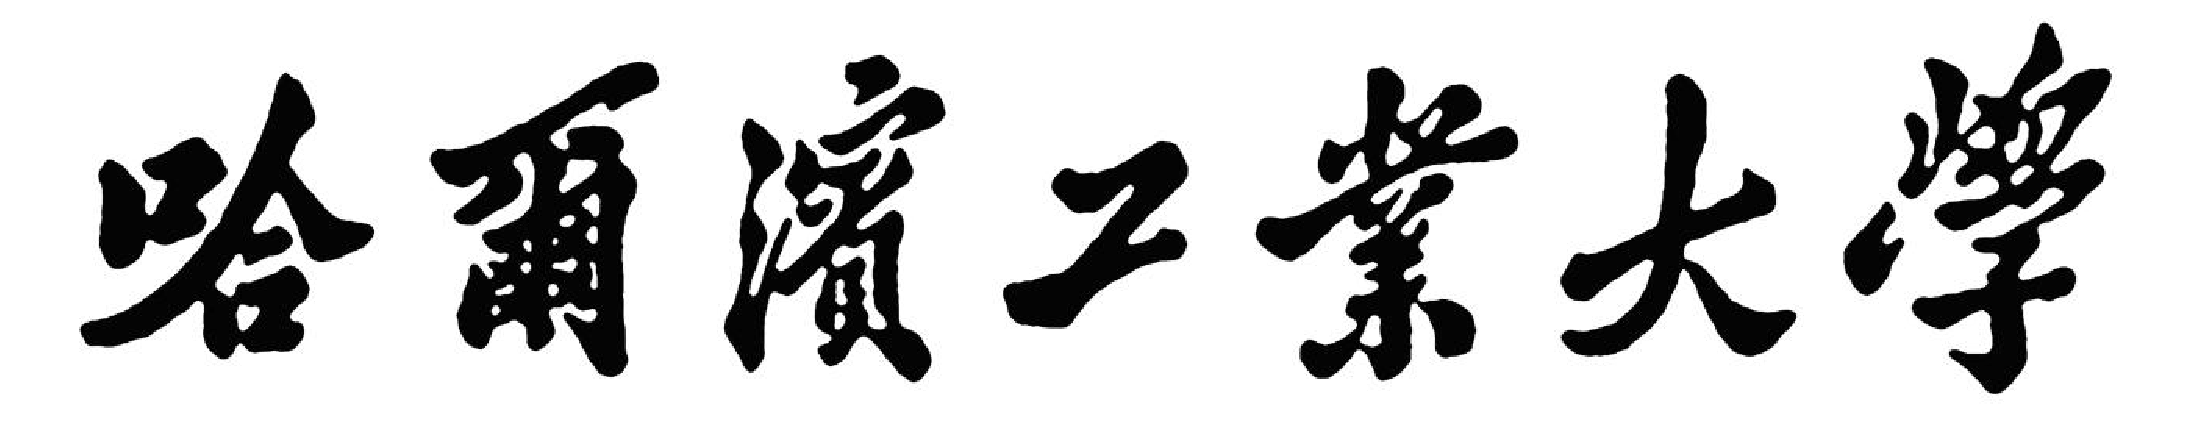
\includegraphics[scale=0.16]{HIT.eps}
\end{figure}		
\vspace{10mm}
\centerline{\zihao{-1}\songti\textbf{毕业设计(论文)开题报告}}
\renewcommand{\CJKglue}{\hskip 0pt plus 0.08\baselineskip}
\vspace{51.5pt}
\zihao{-2}
\begin{center}\songti\textbf{题~目:\@title}\end{center}
\vspace{120pt}
    \zihao{3}
    \hspace*{68pt}{\songti
	\renewcommand{\arraystretch}{1.8}
    \begin{tabular}{l@{}l}
    \textbf{专\hfill 业}     & \rule[-4pt]{200pt}{1pt}\hspace{-326pt}\centerline{\textbf\@subject}\\
    \textbf{学\hfill 生}      & \rule[-4pt]{200pt}{1pt}\hspace{-326pt}\centerline{\textbf\@author}\\
    \textbf{学\hfill 号}  & \rule[-4pt]{200pt}{1pt}\hspace{-326pt}\centerline{\textbf\@stuno}\\
    \textbf{指\hfill 导\hfill 教\hfill 师}     & \rule[-4pt]{200pt}{1pt}\hspace{-326pt}\centerline{\textbf\@supervisor}\\
    \textbf{日\hfill 期} & \rule[-4pt]{200pt}{1pt}\hspace{-326pt}\centerline{\textbf\@date}\\
    \end{tabular}
		\renewcommand{\arraystretch}{1}}
	\vfill
	\vfill
    \centerline{\songti\textbf{\lishu \zihao{-2}哈尔滨工业大学教务处制}}

%%定义内封
\newpage

%%%%%%%%%%%%%%%%%%%%%%%%%%%%%%%%%%%%%%%%%%%%%%%%%%%%%%%%%%%%%%%%%
\thispagestyle{empty}
\zihao{5}\vspace*{2em}
\begin{center}
  \heiti\zihao{3}说\hspace{3em}明
\end{center}
\vspace*{40pt}
	\renewcommand{\arraystretch}{1.25}
    {\heiti\zihao{4}
    \hangindent=2em
	\noindent {\zihao{-3}\textbf{ 一、开题报告主要内容}}
    \begin{enumerate}[leftmargin=36pt]
	\item 课题来源及研究的目的和意义\\ {\songti \zihao{-4}(正文  宋体小4号字,行距1.25倍,段前0行,段后0行)}
	\item 国内外在该方向的研究现状及分析
	\item 主要研究内容
	\item 研究方案
	\item 进度安排,预期达到的目标
	\item 课题已具备和所需的条件、经费
	\item 研究过程中可能遇到的困难和问题,解决的措施
	\item 主要参考文献
    \end{enumerate}
    \noindent  {\zihao{-3} \textbf{  二、对开题报告的要求}}
	\begin{enumerate}[leftmargin=36pt]
	\item 开题报告的字数应在3000字以上。
	\item 参考文献的要求:		
 \end{enumerate}  
\begin{enumerate}
\renewcommand{\labelenumi}{(\theenumi)} 
\songti \zihao{-4}
\item 理工类论文的参考文献一般为10-15篇,其中学术期刊类文献不少于7篇,外文文献不少于3篇(特殊专业可酌情确定明确要求,并报教务处备案);文科、管理类论文,参考文献一般为15-20篇,其中学术期刊类文献不少于12篇,外文文献不少于3篇。近五年的文献数不应少于总数的1/3,应有近两年的参考文献。教材、产品说明书、国家标准、未公开发表的研究报告不宜作为参考资料。
\item 参考文献按在开题报告中出现的次序列出。
\item 参考文献书写顺序:序号 作者.文章名.学术刊物名.年,卷(期):引用起止页。
 \end{enumerate}  
}  
      
%%%%%%%%%%%%%%%%%%%%%%%%%%%%%%%%%%%%%%%%%%%%%%%%%%%%%%%%%%%%%%%%%%%%%%%%%%%%%%%%%%%%%%%
	\renewcommand{\arraystretch}{1}
    \clearpage
}

\makeatother

\frontmatter
% !Mode:: "TeX:UTF-8" 

\title{深度学习在图像识别中的应用}
\subject{自动化}
\stuno{1110410427}
\author{戚锦秀}
\supervisor{杨旭东}
\date{2015年6月29日}



\clearpage
\setcounter{page}{1}

\iffalse
\BiAppendixChapter{摘~~~~要}{}  %使用winedt编辑时文档结构图(toc)中为了显示摘要,故增加此句;
\fi
\cabstract{
深度学习是近年来人工智能研究领域的一个热点,这个机器学习的分支以全连接的深度置信网络和局部连接的卷积神经网络为代表,融合概率图模型、马尔可夫链蒙特卡罗方法等多个技术,其基于大规模数据而训练出的模型在声音识别、图像识别等众多领域中获得了突破性成果。本文主要研究了深度置信网络及卷积神经网络的工作原理,并在MNIST与CIFAR数据集上进行模型的训练,利用GPU与CPU的异构计算在MNIST数据集上取得了98.9\%的识别正确率,在CIFAR-10数据集上取得了62\%的识别正确率。在本文中,我们还讨论了包括降维在内的多个神经网络设计技巧以及实验中发现的一些现象。
}

\ckeywords{深度学习;受限玻尔兹曼机;深度置信网络;卷积神经网络;MCMC;GPU计算}

\eabstract{
Deep learning as a branch of machine learning which is represented by a full  connected neural network  named  Deep Belief Networks as well as a local connected network named Convolutional Neural Networks has drawn lots of attention  in the field of artificial intelligence. Multiple technologies like probabilistic graphical models and Markov Chain Monte Carlo methods have integrated into deep learning nowadays and they help deep learning make a great breakthrough in many AI tasks such as speech  and  image recognition by  training models based on large-scale data. This paper focus on the principles of Deep Belief Networks and Convolution Neural Network s, and we trained some models on the MNIST and CIFAR-10 dataset using DBNs or CNNs. As a result, we achieved 98.9\% recognition accuracy on MNIST dataset and acquires 62\% recognition accuracy on CIFAR-10 dataset with the help of GPU\& CPU-based heterogeneous computing. A number of phenomena found in our experiments and design skills of the neural networks, including dimensionality reduction, will also be discussed in this paper.
}

\ekeywords{deep learning, restricted boltzmann machines, deep belief networks, convolutional neural networks, Markov chain Monte Carlo, GPU computation}

\makecover
\clearpage  % 封面

% 中英目录
\defaultfont
\clearpage{\pagestyle{empty}\cleardoublepage}
\pdfbookmark[0]{目~~~~录}{mulu}
\tableofcontents    % 中文目录
\clearpage{\pagestyle{empty}\cleardoublepage}



\clearpage{\pagestyle{empty}\cleardoublepage}     % 清除目录后面空页的页眉和页脚


\mainmatter\defaultfont\sloppy\raggedbottom

\BiChapter{绪论}{introduction}
\BiSection{课题来源及研究的目的和意义}
x机器学习以及模式识别均属于人工智能范畴,机器学习源自于计算机科学,模式识别源自于工程学,尽管这两者源自于不同的背景,但这两者可以认为是同一个领域下的不同描述\citeup{PRML}。自计算机出生以来,人们一直都在探索一个问题:机器能否实现智能?早期的一部分研究人员试图从事物的机理出发,寻找模式背后的规律,比如在自然语言处理领域,最初人们从分析语法语义开始,企图让机器理解自然语言,并能实现一些类似于翻译之类的工作,但失败了,一个重要的原因是自然语言的规则错综复杂,要摸清其运作机理哪怕以目前的学科水平来看也几乎是难以实现的。

在随后的二三十年里,人类乐观地认为可以找到自然语言背后的运作机理,但实验结果都不尽人意,机理建模这条道路看起来像是一条死胡同。到了上世纪九十年代,统计机器学习开始成为主流,经过二十多年的高速发展,目前基于统计的建模方法成为了主流,而统计机器学习取得的成就远大于上世纪六十年到到九十年代取得的成果,当然这也不排除计算机运算能力的影响。

相比于机理建模,统计机器学习的出发点是从数据出发,建立一个可以刻画已有数据的概率分布,如果将机理建模比作是牛顿力学,那么统计学习就相当于统计力学。事实上,从统计的角度上去解决人工智能问题并不是一个新的想法,早在上世纪七十年代统计学习就已经开始出现。统计机器学习使我们不再需要研究模式背后的运作机理,并且通过它可以实现通用学习。如果说一个事物背后有一个函数决定了它的特性,那么我们不再需要研究这个函数究竟是什么形式,只要有足够多的数据,通过统计方法,选取恰当的模型,我们便可以在一定程度上拟合出这个函数,尽管我们拟合出的函数在大多数情况下都不等价于事物的本质函数,但如果它能在可允许的误差范围内正常工作,这就足够了。

统计机器学习方法的出现,使得工作重点转为寻找合适的模型上,事实上这也是统计机器学习其本质:经验风险最小化\citeup{MLbenzhi}。也就是说,我们应该如何寻找一个合适的模型,使得测试误差最小化?由于模型的选取取决于设计者的意愿,我们既可以选择一个简单的模型,比如线性函数,也可以选择一个复杂的函数,比如高次多项式函数,但是实际问题中,大多数情况下,如果使用简单的线性函数,数据在低维空间中是不可分的,为了使数据变得线性可分,我们可以将数据由低维空间映射到高维空间中,但这种方案引入了庞大的运算以至于计算机难以计算,我们称这种现象为“维数灾难”,即随着维数的线性增加,计算量指数地增大。又或者,我们一开始就不使用线性函数而使用较为复杂的函数比如高斯函数实现非线性分割,但由于我们不知道数据的分布形式,也难以将实际问题中的高维数据可视化,所以除非我们有关于数据分布的先验知识,否则并不知道我们选取的这个复杂的函数是否是合理的。

为了解决维数灾难,我们可以使用核函数,在低维空间中直接计算高维空间返回的结果,避开了高维空间的运算,这种方法也被称之为核方法,比如上世纪九十年代提出的支撑向量机(kernel-SVM)就是一种使用了核方法的分类器。而如果为了避免复杂函数的选取问题,我们可以使用神经网络。神经网络基于一种假说-----智能源自于单一的算法,在神经网络中,我们只需选取激活函数,即所谓的“单一的算法”,然后训练网络的连接权值,从而跳过函数选取步骤。

关于神经网络的表达能力方面,在理论上,柯尔莫格洛夫(Kolmogorov)证明了:只要给予足够多的神经元、合适的激活函数以及恰当的权值,任何从输入到输出的连续映射函数都可以用三层神经网络实现。如果从傅里叶理论上看,则相当于:任何连续函数都可以用足够多的谐波来逼近\citeup{Duda}。

柯尔莫格洛夫的定理说明了神经网络的表达能力与神经网络的层数无关,只与神经元的数目有关,似乎我们没有必要加深网络的深度,但Hastad与Goldmann在1991年提出了以下定理\citeup{learnForAI}

\begin{theorem}\label{theo:NNcomplexity}
为了计算一个函数$f_k \in \mathcal{F}_{k, N}$,深度为$k-1$的单调加权门限电路所需的规模至少为$2^{cN}$,其中常数$c>0$,$N>N_0$
\end{theorem}

由于神经网络与电路的联系十分密切,如果将定理\ref{theo:NNcomplexity} 转化为神经网络的术语,则为:深度为$k$的神经网络所能表达的函数,深度为$k-1$的神经网络为了达到同样的效果至少需要引入指数级规模的节点。

倘若从大脑科学的角度思考,我们已经知道,哺乳动物的大脑是一个深度结构,它可以将输入的模式在多个层次上进行抽象再表达,而每个层次对应着皮层的不同区域。以大脑在视觉系统上的工作机理为例,其工作过程依次经过如下几个步骤:边界检测、基本外形建立、逐渐地完善更为详尽外形\citeup{recognizeShape}。

在定理\ref{theo:NNcomplexity}以及大脑科学的启发下,我们对深度神经网络充满信心,因此神经网络研究人员花费数十年致力于深度神经网络的研究,然而直到2006年之前\citeup{Hinton2006, practicalGuide},我们都难以找到一个较好的算法来训练深度神经网络,其原因一方面是深度神经网络局部最优解繁多,导致深度神经网络比浅层神经网络更容易陷入局部最小值,另一方面则是受计算机运算能力的限制\citeup{diffcultyOfTrain}。

2006年Hinton提出了受限玻尔兹曼机以及深度置信网络的训练方法,通过贪婪逐层地训练\citeup{GreedyLayerWise},成功地实现了第一个深度神经网络,随后深度神经网络又发展处深度卷积网络、稀疏自动编码机\citeup{sparseRepres} 等方法,这些方法被统称为深度学习。目前,深度学习已应用到分类、回归、聚类、降维\citeup{reducingDimensionlity}、自然语言处理、信息检索、机器人学等任务中,且在某些领域中其应用效果已远远超越以前的机器学习方法。


\BiSection{国内外在该方向的研究现状及分析}
x2015年5月,Nature为纪念人工智能60周年开辟了"人工智能与机器人"专题,回顾了过去的研究历程与当今的研究热点,其中深度学习作为一个热点被加以介绍\citeup{nature2015}。目前深度学习在国内外都受到广泛关注,新的深度学习算法源源不断地被提出,在不久的将来,深度学习将会取得更多的成功。
\BiSubsection{神经网络与深度学习的发展状况}
x数十年来,神经网络研究人员在神经科学上付出了巨大心血,其研究之深入,范围之广,内容之繁杂是别的机器学习方法所难以企及的。我们今天看到的深度学习只是神经计算科学中的冰山一角,在它之下,是几十年探索积累起来的失败经验,这些模型中不乏观点新颖却无法工作的模型。这么多年来研究人员试图将神经网络理论化,然而到目前为止这项工作依然没有实现。
\BiSubsection{感知器时期}
x关于神经网络的想法由来已久,远在1800年人们已经开始研究神经网络,1943年心理学家Warren McCulloch与数理逻辑学Walter Pitts在总结前人关于神经工作原理的基础上将神经元工作数理化,随后冯·诺依曼在领导计算机设计时试图使用神经网络的形式而不是目前的指令形式\citeup{fengnuoyiman},限于当时科技水平限制最后并没有采用神经网络的方案。随着二十世纪六十年代控制论兴起以及计算机的出现,联接主义学者迫切地期待建立一个可用的神经网络数学模型,在这个环境中,受Warren McCulloch与Walter Pitts两人工作的启发下,Frank Rosenblatt提出了第一个神经元模型----感知器\citeup{overview},这标志着神经网络进入第一次浪潮。
\begin{figure}[!htbp]
\centering
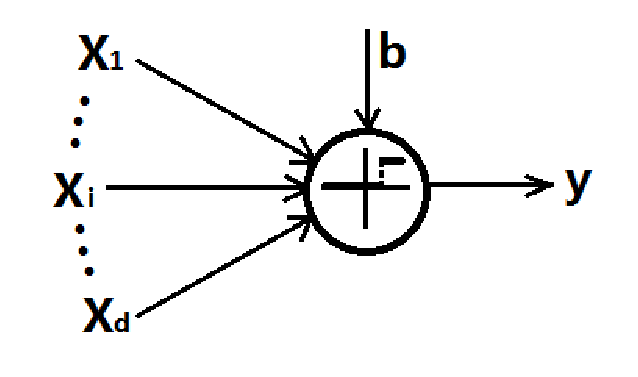
\includegraphics[width=0.33\textwidth]{NNnode.eps}
\caption{感知器模型}
\label{img:NNnode}
\end{figure}

如图\ref{img:NNnode} 所示,在感知器中,含有$d$个输入和1个输出,其中非线性激活函数为阶跃函数,即
\begin{equation}
y = \left\{
\begin{array}{cc}
1 & \text{~~~~若$\theta^Tx - b \geq 0$}\\
0 & \text{~~~~其他}\\
\end{array}
\right.
\end{equation}
式中$b$为偏置项,有时也称之为阈值。如果从神经科学的角度上解释,在感知器中,向量$x$相当于神经元接收到的刺激,而$\theta^T x$相当于刺激的叠加。当总的刺激量到达一定阈值$b$时,神经元被激活,即$y=1$,否则神经元对刺激不作反应,即$y=0$。

伴随感知器一同被提出的还包括感知器训练算法,其方法借鉴了生理学中关于反馈方面的思想,通过引入奖励与惩罚的概念,当某个训练样本被正确分类时,参数维持不变,若该样本被错误分类,则通过惩罚项对对参数进行更新\citeup{MLbenzhi}。

得益于非线性的激活函数,感知器网络可以实现逻辑功能以及非线性分类任务。例如,在输入维度为2的感知器网络中,若网络参数$\theta = [-2, -2]^T$,偏置$b = 3$,此时,这组参数构成的感知器即为门电路中的与非门。由于与非门可以构成与、或、非三种基本逻辑门,而这三者又可以构成所有的逻辑函数,因此我们有理由相信,恰当的感知器网络可以实现逻辑功能。事实上,六十年代感知器网络的提出,也确实解决了一些简单的人工智能任务。

神经网络第一次浪潮只持续了大约十年左右,究其原因,一方面,六十年代是电子计算机刚刚兴起的年代,人们更多地关注于计算机,导致感知器网络得不到重视,另一方面,限于电子管及早期晶体管的工艺,耗费大量的资源来建立一个感知器网络似乎也不太现实。此外,人们一直没有找到一种能较好地训练多层感知器网络的算法,导致了大批神经网络学者对其失去信心,因此,在六十年代末期,神经网络的研究进入第一个低谷。

\BiSubsection{反向传播时期}
x神经网络研究在八十年代进入第二次浪潮,最重要的原因是1986年Hinton、Remelhart和Williams等人提出了反向传播算法\citeup{bpalg},首次在手写数字识别任务上使用反向传播训练的神经网络,取得了较好的效果。此外,大规模集成电路的发展以及sigmoid等新的激活函数的应用也很大程度程度上推动了神经网络的发展。

反向传播算法通过链式求导,将偏导数从高层传送回低层,使得多层感知器网络中可以使用简单的梯度下降方法进行训练,尤其是在三层感知器网络中效果显著。随后,感知器网络也改名为神经网络,尽管如此,神经网络只是人为主观地对神经元建模,其本质与生物的神经系统是没有太大联系的,例如神经具有局部稀疏性而神经网络是非局部的,因此神经网络在生物学上被批评为缺乏真实性。

在这个时期,新的模型不断地被提出,比如使用Hebb规则全连接的反馈网络Hopfield网络\citeup{information}、将Hopfield网络随机化后的玻尔兹曼机\citeup{learnForBM}、具备模式变换不变性的卷积网络等\citeup{Duda},此外,一些新的技术例如快速传播、共轭梯度等也被应用到神经网络中。

九十年代人们开始尝试建立深度神经网络,但随着网络深度的加大,局部最优解增多,在参数没有被恰当地初始化的情况下,使用反向传播算法进行简单的梯度下降容易陷入局部极小值,人们难以找到一种较好的方法来训练深度网络。在硬件方面,九十年代计算机的计算能力仍不足以满足深度神经网络中大规模的运算。此外,同时期被提出的SVM方法可以在较少运算的前提下实现高性能的分类,因此,在九十年代中期,神经网络进入第二次低谷。

\BiSubsection{深度学习时期}
x深度神经网络的僵局一直持续到2006年,Hinton与Osindero在深度置信网络中使用一种无监督的逐层贪婪预训练受限玻尔兹曼机,使得权值被初始化到一个合适的位置,随后对整个网络使用全局的反向传播进行有监督的微调,在MNIST手写数字识别任务上超越了已有的记录\citeup{Hinton2006},随后,在受限玻尔兹曼机的基础上又发展出了稀疏编码与自动编码机等方法。深度置信网络是一种无监督学习,对应的,由LeCun等人提出的深度卷积网络实现了在深度结构下的有监督学习\citeup{lecun1989backpropagation,lecun1998gradient},成为第一个真正意义上的深度结构。

自2006年以来,深度学习的研究持续升温\citeup{frontierInAI,learnDeepModels},Google、Facebook、Microsoft等公司以及麻省理工、斯坦福大学、多伦多大学等高校投入大量资源到深度学习的相关研究中,麻省理工大学在2013年将深度学习评为十大突破技术的榜首\citeup{baidu}。由于深度学习需要训练样本容量足够大,而近年来大数据时代的到来,人们难以处理规模如此庞大的数据,所以某种程度上,深度学习与大数据是相辅相成的。

2012年前后,国内各大公司逐渐投入到深度学习相关的研究中,百度于2013年开展百度大脑计划,成立“深度学习研究院”,这是百度首次成立研究院,并于2014年邀请了深度学习的领军人物吴恩达作为首位院长。腾讯公司于2014年开发的Mariana平台将致力于研究深度学习在语音识别、图像识别和广告推荐上的应用。2015年京东将开展“JIMI”机器人项目,企图将深度学习应用到人工客服上。


\BiSection{深度学习在人工智能上的应用}
x深度学习在人工智能领域正在取得重大进展,利用这套技术解决了历史遗留的大量问题,目前已被应用到科学、商业、政策上。除了在传统的声、图、文领域深度学习掀起巨浪外,深度学习逐步开始渗入到生物学等其他领域。
\BiSubsection{语音识别}
x传统的语音识别一般使用混合高斯模型(GMM)或隐马尔可夫模型(HMM)\citeup{Duda},这些模型一般都比较简单,难以实现较高的正确率。Microsoft于2009年与Hinton在语音识别方面展开合作,并于2011年实现了深度学习在语音识别上的应用,该应用已经投入到WindowsPhone的语音识别“小娜”中。Google、百度也开展语音识别框架的改革,Google使用4$\sim$5层的神经网络,而百度使用9层的神经网络\citeup{baidu}。使用深度神经网络实现的语音识别在错误率上要比传统方法的错误率相对少$20\%\sim  30\%$左右。

\BiSubsection{图像识别}
x在声、图、文三个领域中,深度学习在图像识别上对识别效果的提升最显著。在MNIST手写数字识别任务中,使用传统识别方法的正确率一般为98\%左右,使用SVM能达到98.6\%的正确率,而使用深度学习方法在最好的情况下能达到99.79\%的正确率。在ImageNet1000任务中,对于1000个类别的识别,随着深度学习的研究进展,其识别效果分别经历了72\%、85\%、89\%、93\%等阶段,截止到2015年1月,由微软亚太研究院实现的最好效果为96.06\%\citeup{MS2015}。在SVHN街景门牌号的识别任务中,Google通过11层的神经网络对门牌号实现了97.84\%的正确率,这个系统已经帮助Google从街景中分析出全球近 1 亿个门牌号。

\BiSubsection{自然语言处理}
xMicrosoft于2012年在天津展示了使用深度学习训练的同声翻译系统,其英中翻译较传统方法更为流畅。然而,目前在自然语言处理领域,深度学习取得的效果并没有显著超越传统方法。相比于图像识别以及语音识别,自然语言处理一个难点在于上下文,尽管深度学习被认为是一种特征学习,但这种特征学习似乎并没有实现可以联系上下文的功能。自然语言处理在近期广受关注,深度学习研究人员认为下一个突破口将会出现在自然语言处理上。







\BiChapter{控制论与机器学习}{CSandML}
控制论其本质,在于利用已有的信息抑制系统熵的增加\citeup{weina},需要注意的是,这里的熵并不是指热力学中的热力熵或信息论中的信息熵,而应理解为熵的原始定义,即对混乱的度量。既然是度量,便需要一个准则,正如测量一个物体的长度需要一把刻度尺,但不同的刻度尺将得到不同的测量结果,同理,对混乱的不同定义,也将得到不同的控制效果。例如,在温度控制系统中,让温度保持在一个较高的温度或较低的温度均是抑制熵增的行为,因为两者对熵的定义不同。对于孤立系统,熵总是朝着增加的方向移动,但也有例外,此时系统必须是非孤立的,能够收到外界的控制,比如有机体具有熵减趋势,因为DNA是有序的(尽管我们目前仍无法完全理解它),其中起到控制作用的外力是自然选择。控制论所要做的,便是引入外力作用,即反馈,或者说控制环节,以之降低系统的混乱程度,得到我们的期望输出。

\BiSection{白盒模型与经典控制论}
x经典控制论中,为了实现对一个系统的控制,我们往往需要先由系统的结构开始分析,利用牛顿力学、电磁原理、热力学等物理原理对系统特性建立微分方程,将其转换为复域的传递函数后,再利用根轨迹或频域分析设计控制环节。如图\ref{img:RLC} 所示的简单RLC网络中,假定我们以$u_i(t)$作为输入,$u_o(t)$作为输出,那么此时我们所拥有的信息是整个系统的结构,所需要抑制的混乱就是控制$u_0(t)$朝着我们的期望输出迈进。

\begin{figure}[htbp]\label{img:RLC}
\centering
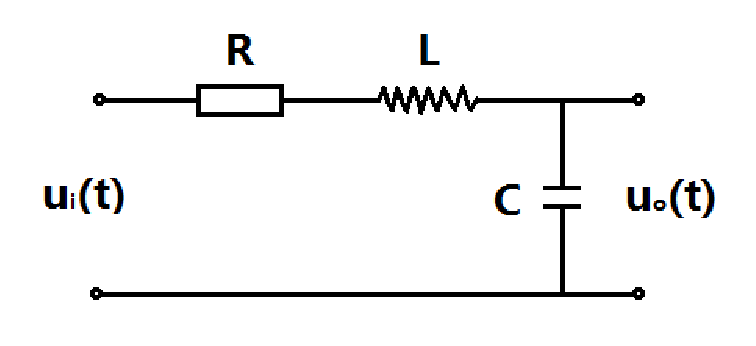
\includegraphics[width=0.5\textwidth]{CSandML/RLC.eps}
\caption{简单的RCL网络}
\end{figure}

由于这个系统的结构是已知的,整个系统对于我们而言相当一个白盒。为此,我们可以很容易地根据基尔霍夫回路电压定律建立方程
\begin{equation}\label{equ:KVL}
u_L(t) + u_R(t) + u_o(t) = u_i(t)
\end{equation}
进一步利用电感特性、电容特性、欧姆定律,式\eqref{equ:KVL}可以进一步推导为
\begin{equation}
LC\frac{d^2u_o(t)}{dt^2} + RC\frac{du_o(t)}{dt}  + u_o(t) = u_i(t)
\end{equation}
此时,输入输出的微分方程已建立,下一步便是经典控制论的内容,我们并不打算继续展开细说。在这个例子中,我们可以看出,白盒模型对整个系统是了如指掌的,是可以对其建模的。此时,“利用已有信息抑制系统的熵增”相当于,对系统建立传递函数(利用已有信息),设计控制环节使我们能得到期望输出(抑制熵增)。

\BiSection{灰盒模型与系统辨识}
x牛顿一生的工作对自然科学的贡献是无以衡量的,但牛顿生活的时代忽视了一些重要的东西---统计的概念。在牛顿力学中,有一个前提,系统的状态是可测量的,因此,牛顿力学基于一个已给定的精确初始状态之上对系统分析。然而,物理的测量从来都不是精确的,我们对世界的观察也总是片面而不确定的,世界对我们而言是未知的,我们无法完全确定事物的运作机理。例如图\ref{img:RLC} 中的电阻R,R=50$\Omega$ 并不是一个严谨的说法,我们不知道物体细分到最小粒子(如果存在的话)后事物是否变得精确,但就目前人类所拥有的知识而言,阻值为50$\Omega$的电阻是不存在的。我们平常所说的50$\Omega$电阻只是一个统计概念,即电阻在50$\Omega$左右的统计结果。延伸到整个系统,图\ref{img:RLC} 的网络也变得不确定,R、L、C均是不精确的值,此时系统变为一个灰盒模型。所谓灰盒模型,即系统的一部分内容是未知的,另一部分内容是已知的的,例如这里,尽管R、L、C的精确值是未知的,但我们依然可以知道其数值的大致范围。

倘若我们再推广一步,R、L、C的大致范围我们也不知道,如何设计该系统的控制环节便是系统辨识所要研究的内容。系统辨识领域中的一个重要的话题是如何解析出一个含有未知参数的系统结构,如果我们可以获取系统的输入输出样本,利用这些样本,配合上含有未知参数的系统结构方程,采取恰当的拟合方法,如最小二乘以及极大似然等,最后可以获取未知参数的近似解,使得这个灰盒模型的灰色褪去(但不会褪为白盒模型),进一步便可设计系统的控制环节。
\BiSection{黑盒模型与统计机器学习}
x白盒模型与灰盒模型的讨论均是基于一个前提:我们知道系统整体模型框架,只是某些参数有可能是未知的。但这个前提在实际生活中往往是不成立的,很多时候,我们非但不知道系统的参数,甚至连系统的模型也知之甚少,此时的系统相当于一个黑盒,我们无法了解其内部结构。例如,判断一封100字的邮件是否为垃圾邮件,假设这个行为可以用一个函数来描述,即这个决策背后存在一个真理(或者说函数),通过它,我们输入100个字符,函数的输出告诉我们这封邮件是否为垃圾邮件 ,那么我们便可以通过这个函数来描述这个系统。可以肯定的值,这个函数在邮件完全可分(即不存在一些可能是或可能不是垃圾邮件的情况)的前提下是存在的,因为字符编码是有限的,只需穷举即可得到这个函数的决策面。但这个方法并不现实,假使所有的汉字只有2000个,那么100字的中文邮件将有$2000^{100}$种可能,要穷举是不可能的。另一种做法是寻求语法结构,先对这100字进行分词,再进行语义分析,这个过程也可以描述为一个函数映射过程:假设函数$f(x)$代表分词,$g(x)$代表语义分析,$y$代表系统输出,那么系统的模型可以表述为$y = g[f(x)]$。这种想法早在二十年前就被抛弃,因为自然语言含有强烈的上下文气息。例如在“冬天能穿多少穿多少,夏天能穿多少穿多少”这个例子中,同一句“能穿多少穿多少”在不同的上下文中含有不同的意义。尽管我个人认为这种上下文背后也必然存在一个因果关系,但这种因果关系是在是太难寻找了,所以这种方法也不是一个可行的方案。

统计机器学习的做法是,假定一个模型(这个模型与系统本质的模型关联并不大),利用大量样本训练假设的模型,最后将训练完毕的模型作为本质模型的逼近。与之前讨论的系统辨识相比,两者在训练阶段是类似的,均是利用样本进行参数整定,不同点在于,系统辨识是训练带有强烈先验的模型(比如由具体物理原理推导出的传递函数)的参数,而统计学习训练的是假设模型(比如高斯模型、隐式马尔可夫模型、神经网络、支持向量机等)的参数。

回到垃圾邮件分类的例子中,统计机器学习的一种解决方案是利用朴素贝叶斯分类,这种方法中,所假设的模型是朴素贝叶斯模型。我们首先建立一个含有$d$个元素的垃圾邮件特征字典,比如$\{$ 购买、大促销、店庆$\cdots \}$,此时,任何一封邮件都可以用一个$d$维列向量表示。例如,某封邮件在字典中的元素只包含“购买”,而其他的元素均不包含,那么这封邮件便可以表示为
\begin{equation}
x = [1, 0, 0, \cdots , 0]^T
\end{equation}

如果我们有大量垃圾邮件样本,我们不难统计出字典中各个元素在垃圾邮件中的出现概率$p(x_i|y=1)$,其中,$y$代表样本的标签,若该样本是垃圾邮件,则$y=1$,反之$y=0$,$x_i$代表字典中的第$i$个元素,例如,我们的字典中,$x_1$ = “购买”。建立样本的描述方式后,我们采用朴素贝叶斯公式,计算样本为垃圾邮件时的概率分布
\begin{equation}\label{naiveBayess}
\begin{split}
p(x|y=1)&= p(x_1, x_2, \cdot, x_d|y=1)\\
&=p(x_1|y=1)p(x_2|y=1)\cdots p(x_d|y=1)
\end{split}
\end{equation}
显然,式\eqref{naiveBayess}在数学上只有在$x_i$均独立时才成立,而本质上,$x_i$并不是独立的(因为存在上下文),这里本应使用全概率公式,而我们之所以假设$x_i$独立的原因是这样做可以降低模型的复杂度。所以说,在统计学习中,假设模型与本质模型的关联往往不大。

模型训练完毕后(即计算$p(x_i|y=1)$),对于一封新收到的邮件,我们只需使用贝叶斯公式即可计算该邮件是垃圾邮件的概率
\begin{equation}
\begin{split}
p(y=1|x) &= \frac{p(x|y=1)p(y=1)}{p(x)}\\
&=\frac{\prod_{i=1}^d p(x_i|y=1)}{\prod_{i=1}^d p(x_i|y=1) + \prod_{i=1}^d p(x_i|y=0)}
\end{split}
\end{equation}
统计学习更像是一种假设检验,本例子中的朴素贝叶斯,完全抛弃了语义分析,这并不符合自然语言的原理。但实际中,尽管这个模型并不是本质模型,但逼近效果足以让人接受,能工作得很好,因此被很多邮件厂商所采用。

\begin{figure}[htbp]
\centering
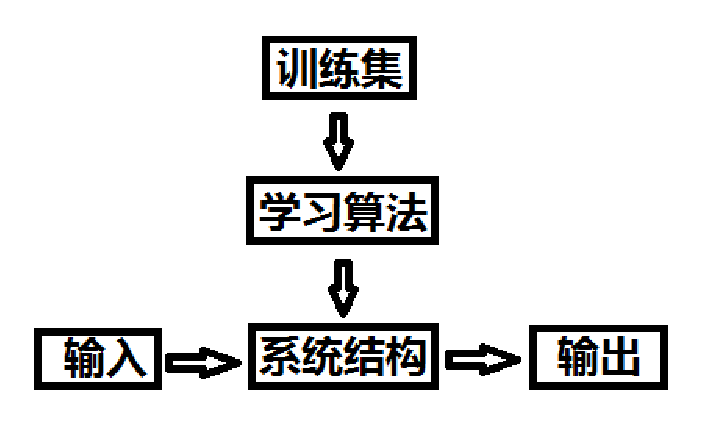
\includegraphics[width=0.4\textwidth]{CSandML/ML.eps}
\caption{机器学习系统框图}\label{img:ML}
\end{figure}

如果一定要对机器学习下一个定义,我认为Tom.Mitchell的描述比较恰当:对于某类任务T和性能度量P,如果一个计算机程序在T上以P衡量的性能随着经验E而自我完善,那么我们称这个计算机程序从经验E中学习\citeup{tomML}。如果将这段话转化成系统框图,则如图\ref{img:ML} 所示。

\BiSection{本章小结}
x精确性只存在于数学中,现实世界充满了不确定性,难以寻找事物背后的机理。统计学习绕过这套机理,根据设计者的意愿,假设一个模型,利用这个模型逼近事物的机理,相当于把世界看成一个黑盒,并不打算去探索黑盒的内部结构,而是仿造一个黑盒来模拟其工作原理。
\BiChapter{受限玻尔兹曼机}{RBM}\label{chapter:RBM}
统计学习并不在乎事物的本质是什么,我们更关心的是数据的分布是怎样的,为了描述数据的分布,我们往往引入各种各样的模型刻画这种分布,比如,贝叶斯决策论中我们引入多维高斯分布,支持向量机中我们引入最大间隔分离面等。对于同一个任务,采用不同的模型得到的结果是不一样的,机器学习与模式识别的一个不同点在于,机器学习更注重统计,模式识别更注重于模型。例如,对于同一个任务,机器学习学者可能会假设出多个模型,再根据模型选择理论选取一个最优的模型,而模式识别学者更倾向于先大致分析这个任务更适合使用哪个模型,选取后仔细优化这个模型。尽管两者有一定的差异性,但很多方面两者是共通的,比如神经网络。神经网络并不依赖于具体的任务,也就是说,语音识别可以用神经网络处理,图像识别也可以用神经网络处理,之所以能这样做的一个原因是,神经网络的内部对于我们而言是透明的,如果我们只看重结果,希望有一个模型可以在给定一个输出的时候输出一个决策结果,不需要关心这个结果是怎么得到的,那么神经网络是一个很好的选择。神经网络的种类众多,一个分支是玻尔兹曼机,这种网络灵感源自统计物理中的玻尔兹曼分布与伊辛模型,随后,在这种网络的基础上又发展出一套受限玻尔兹曼机,通过这些网络,都可以建立数据的概率分布描述。
\BiSection{伊辛模型}
x伊辛模型是统计物理中描述物质相变的一种模型\citeup{information},是一个相互磁耦合的自旋阵列。比如在铁这种物质中,当温度降到某个程度,微观原子的自旋会表现出一定的倾向性,从而在宏观上产生磁矩,而当温度升高到一定程度时,其自旋就变得随机。

假设某个伊辛模型中有$N$个自旋的原子,对于每个原子,其状态只能取$+1$或$-1$,我们用向量$s$来表示所有原子的状态,亦即$s$代表这个伊辛模型的状态,那么我们定义该伊辛模型处于状态$s$下的能量函数为\citeup{information}
\begin{equation}
E(s; W, H) = -~\Big[\frac{1}{2} \sum\limits_{i, j = 1}^{N} w_{ij}s_is_j + \sum\limits_j Hs_j\Big]
\end{equation}

式中, $w_{ij}$代表原子$i$和原子$j$之间的耦合,如果$i$和$j$是相邻的,那么$w_{ij} = C$,否则$w_{ij} = 0$,如果常数$C>0$,那么这个模型是铁磁性的,否则是反铁磁性的。常数$H$代表作用场,$E(s; w, H)$代表能量函数,对于一般化的能量函数,我们也称之为Lyapunov函数。如果将这个能量函数推广到$H$和$W$不是常数的情况,即\citeup{information}

\begin{equation}\label{eq:energyFunction}
E(s; W, H) = -~\Big[\frac{1}{2} \sum\limits_{i, j = 1}^{N} w_{ij}s_is_j + \sum\limits_j h_js_j\Big]
\end{equation}
此时我们将得到一个物理学家称之为“自旋玻璃”的模型,这也是神经网络中的“Hopfield网络”。

\BiSection{玻尔兹曼机}
x在统计物理中,对于一个具有一定自由度的物理系统,其系统的状态是具有随机性的而不是固定的(比如房间中的氧气分子分布),假设系统处于某个状态$i$的概率为$p_i$,那么当系统与外界达到热平衡时,其概率分布为
\begin{equation}\label{zhengzefenbu}
p_i = \frac{1}{Z_T} e^{-E_i / T}
\end{equation}
式中,$T$代表系统所处的温度,$E_i$代表系统处在$i$状态下的能量,$Z_T$是在$T$温度下为了使得概率满足柯尔莫果洛夫第二公理的归一化常数。这个分布也称之为正则分布或吉布斯分布。

在机器学习中,我们往往自定义一个能量函数,然后通过正则分布建立模型,通过这种基于能量的模型来对数据进行分析。所以正则分布可以看做是机器学习与统计物理间的桥梁。

如果将式\eqref{eq:energyFunction}中的作用场去掉,并改写成矩阵形式,则得到玻尔兹曼机中的能量函数
\begin{equation}
E(s; W) = -~\frac{1}{2} s^TWs
\end{equation}

事实上,在机器学习中我们并不关心常数$T$,则玻尔兹曼分布为
\begin{equation}
p_i = \frac{1}{Z} e^{-E_i}= \frac{1}{Z} \exp\Big[\frac{1}{2} s^TWs\Big]
\end{equation}

对于一个数据对象,假设我们能观察到$n$维特征,但不仅仅代表这个数据只含$n$维特征,因此我们往往引入隐含特征的概念,假设对于一个对象,我们能观察到$v$个特征,那么我们用$v$个节点来表示这些特征,又假设我们自定义隐含的特征为$h$个,那么我们用$h$个节点来代表这个特征。比如图\ref{img:BM} 代表了含有4个可见节点和2个隐含节点的玻尔兹曼网络。
\begin{figure}[htbp]
\centering
\subfigure{\label{BM1}}\addtocounter{subfigure}{-2}
\subfigure{\subfigure[未拓扑前的玻尔兹曼机]
			{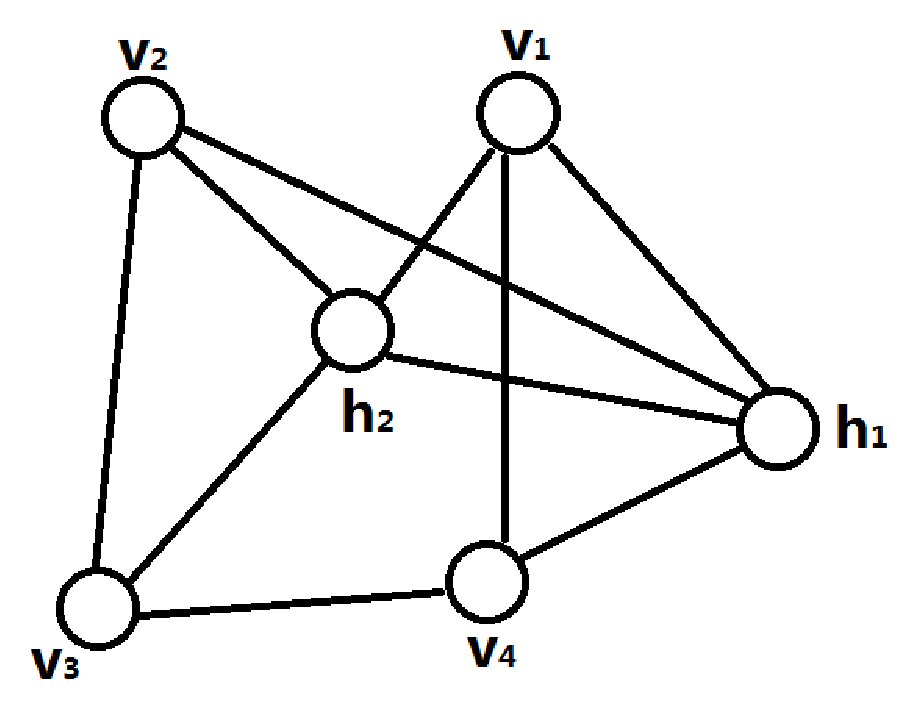
\includegraphics[width=0.3\textwidth]{BM1.eps}}}
\subfigure{\label{BM2}}\addtocounter{subfigure}{-2}
\subfigure{\subfigure[拓扑后的玻尔兹曼机]
			{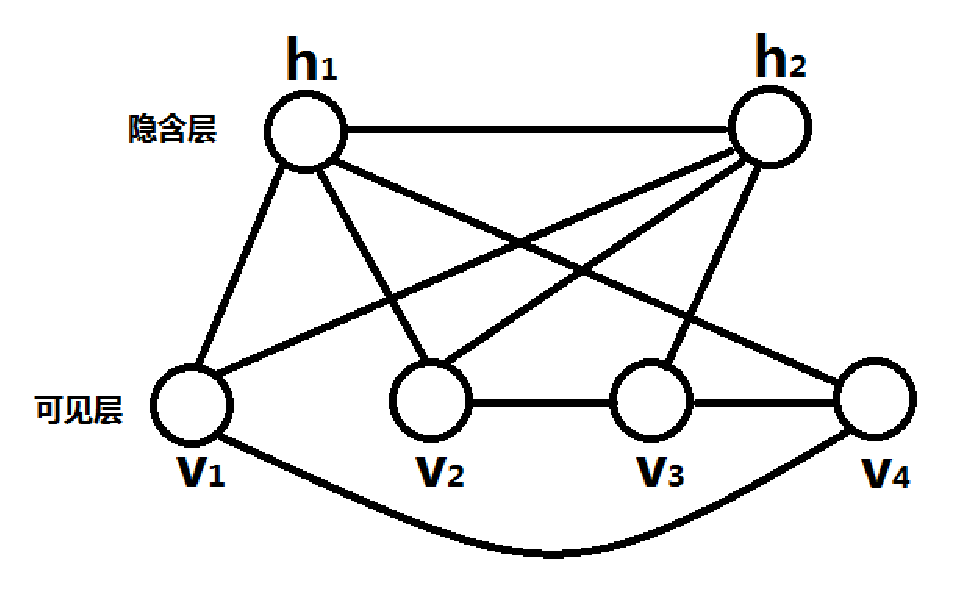
\includegraphics[width=0.4\textwidth]{BM2.eps}}}
\caption{玻尔兹曼机网络构型}
\label{img:BM}
\vspace{-1em}
\end{figure}

由图\ref{img:BM} 可见,在玻尔兹曼机中,可见节点与可见节点之间、隐含节点与隐含节点之间是可以有连接的,因此这是一个反馈网络。层内节点有连接可以大大地增强网络的表达能力,但是也大大地增加了网络的训练难度,因此玻尔兹曼机并没有非常成功地解决人工智能的任务。

\BiSection{受限玻尔兹曼机}
x在受限玻尔兹曼机(Restrict  Boltzmann Machine,RBM)中,我们取消层间连接,从而出发后经过若干次“移动”也无法回到原点,因此RBM也可以认为是一个有向无环图。其网络结构图\ref{img:RBM} 所示。

\begin{figure}[!htbp]
\centering
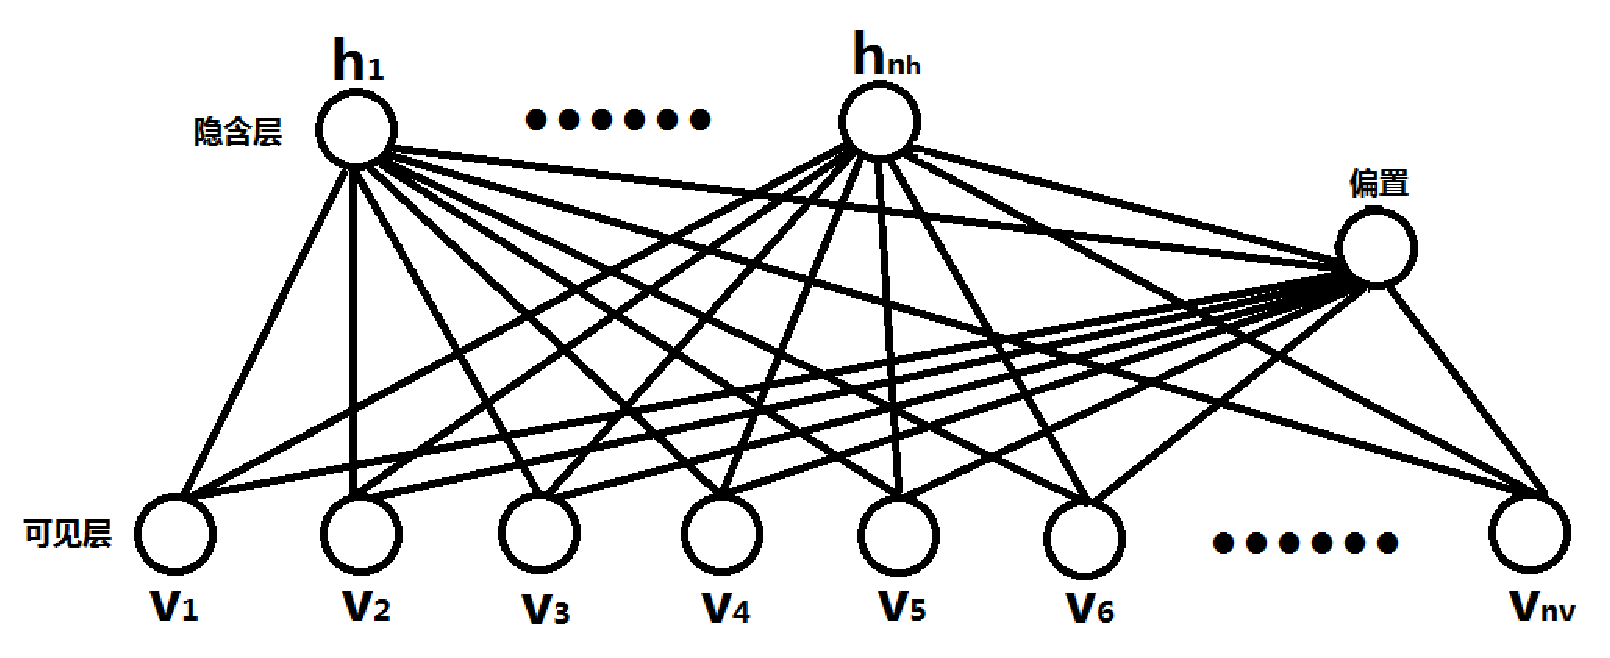
\includegraphics[width=0.7\textwidth]{RBM.eps}
\caption{RBM网络构型}
\label{img:RBM}
\end{figure}

为了方便往后的讨论,我们约定网络参数的数学符号如下

\begin{equation}
W_{n_h \times n_v } = \left[               %左括号
\begin{array}{cccc}  
w_{1,1} & w_{1,2} &\cdots & w_{1, n_v}\\  
w_{2,1} & w_{2,2} &\cdots & w_{2, n_v}\\
\vdots  & \vdots & \ddots  & \vdots\\
w_{n_h, 1} & w_{n_h, 2} & \cdots & w_{n_h, n_v}
\end{array}
\right]~~~~%%%%%%%%%%%%%%%%%%%%
v = \left[   
\begin{array}{cccc}  
v_1\\  
v_2\\
\vdots\\
v_{n_v}
\end{array}
\right]~~~~%%%%%%%%%%%%%%%%%%%
h = \left[   
\begin{array}{cccc}  
h_1\\  
h_2\\
\vdots\\
h_{n_h}
\end{array}
\right]~~~~%%%%%%%%%%%%%%%%
b_v = \left[   
\begin{array}{cccc}  
b_{v_1}\\  
b_{v_2}\\
\vdots\\
b_{v_{n_v}}
\end{array}
\right]~~~~%%%%%%%%%%%%%%%%%%%%%% 
b_h = \left[   
\begin{array}{cccc}  
b_{h_1}\\  
b_{h_2}\\
\vdots\\
b_{h_{n_h}}
\end{array}
\right]
\end{equation}
式中,$W_{n_h \times n_v }$代表网络的权值参数,$w_{ij}$代表第$i$个隐含节点到第$j$个可见节点间的连接权值,因此$W_{n_h \times n_v }$的第$i$行代表了通向$h_i$的所有连接的权值, 第$j$列代表了通往$v_j$的所有连接的权值。 $v$代表可见节点的状态,$h$代表隐含节点的状态,$b_v$代表隐含层到可见层的偏置,$b_h$代表可见层到隐含层的偏置。

在RBM中,我们定义其Lyapunov函数如下\citeup{energyBased}:
\begin{equation}\label{eq:RBMenergy}
E(v, h) = - \sum\limits_{i=1}^{n_v}b_{v_i}v_i - \sum\limits_{j=1}^{n_h}b_{h_j}h_j -  \sum\limits_{i=1}^{n_v} \sum\limits_{j=1}^{n_h} h_j w_{j, i}v_i
\end{equation}
若将\eqref{eq:RBMenergy}写成矩阵形式,则为:
\begin{equation}
E(v, h) = -b_v^T v - b_h^T h - h^T W v
\end{equation}
由正则分布的定义\eqref{zhengzefenbu},我们可以得到$v$,$h$的联合分布为
\begin{equation}\label{lian he fen bu}
p(v, h) = \frac{1}{Z} e^{-E(v, h)}
\end{equation}
其中配分函数$Z$为
\begin{equation}\label{partionFunc}
Z = \sum\limits_{v, h}e^{-E(v, h)}
\end{equation}
由于实际中我们往往只能观察到可见节点,因此对联合分布\eqref{lian he fen bu}边缘化得
\begin{equation}\label{p_x1}
p(v) = \sum\limits_h \frac{1}{Z}e^{-E(v, h)} = \frac{1}{Z}\sum\limits_h e^{-E(v, h)}
\end{equation}
这个$ p(v) $总可以写成如下形式:
\begin{equation}\label{p_x2}
p(v) = \frac{e^{-F(v)}}{Z}
\end{equation}
式中,我们称$ F(v)  $为自由能函数\citeup{learnForAI},由式\eqref{p_x1}与\eqref{p_x2},我们不难推出$ F(v)  $为
\begin{equation}\label{freeEnergyDef}
F(v) = -\ln\sum\limits_h e^{-E(v, h)}
\end{equation}

为了继续我们往下的讨论,我们不加证明地引入关于受限玻尔兹曼机的一个定理:
\begin{theorem}\label{theo:iid}
在RBM中,在给定可见元状态时,隐含元的激活条件独立;反之,在给定隐含元状态时,可见元的激活条件独立。
\end{theorem}

此外,我们还需引入一些记号
\begin{equation}
h_{-k} = (h_1, h_2, \cdots, h_{k-1}, h_{k+1},\cdots, h_{n_h})^T
\end{equation}
\begin{equation}
\alpha(k) = b_{h_k} + \sum\limits_{i=1}^{n_v} w_{k, i}v_i
\end{equation}
\begin{equation}
\beta(v, h_{-k}) = \sum\limits_{i=1}^{n_v} b_{v_i}v_i + \sum_{\substack{j=1\\ j\neq k}}^{n_h} b_{h_j}h_j +  \sum\limits_{i=1}^{n_v}  \sum_{\substack{j=1\\ j\neq k}}^{n_h} h_j w_{j, i}v_i
\end{equation}
即$h_{-k}$代表除$k$外的所有隐含元状态,$\beta(v, h_{-k})$代表除$h_k$外所有节点构成的能量函数。因此,总的能量函数\eqref{eq:RBMenergy}可以写为
\begin{equation}
E(v, h) = -\beta(v, h_{-k}) - h_k \alpha(k)
\end{equation}

下面我们来推导隐含层的激活函数,在给定可见节点状态时,对于节点$h_k$,其激活概率为
\begin{equation}\label{equ:prob}
P(h_k = 1| v)
\end{equation}
由定理\ref{theo:iid},式\eqref{equ:prob}等价于
\begin{equation}
\begin{split}
P(h_k = 1|h_{-k}, v) &= \frac{P(h_k = 1, h_{-k}, v)}{P(h_{-k}, v)}\\
&= \frac{P(h_k = 1, h_{-k}, v)}{P(h_k=0,h_{-k} , v) +P(h_k=1, h_{-k} , v)  }\\
&=\frac{1}{1 + \exp\Big(-E(h_k = 0, h_{-k}, v) +E(h_k = 1, h_{-k}, v)  \Big)}\\
&= \frac{1}{1 + \exp\Big[  \Big(\beta(v, h_{-k})+ \alpha(k)\cdot 0\Big) + \Big(-\beta(v, h_{-k})- \alpha(k)\cdot 1\Big)  \Big]}\\
&= \frac{1}{1 + e^{-\alpha(k)}}\\
&=sigmoid\Big(\alpha(k)\Big)
\end{split}
\end{equation}
因此,给定可见层状态时,隐含元$k$的激活概率为
\begin{equation}\label{p(h_k|v)}
P(h_k =1| v) = sigmoid(b_{h_k} + \sum\limits_{j=1}^{n_v}w_{k, j}v_j)
\end{equation}
同理可推导在给定隐含层状态时,可见元$k$的激活概率为
\begin{equation}\label{p(v_k|h)}
P(v_k = 1|h) = sigmoid(b_{v_k} + \sum\limits_{i=1}^{n_k}w_{i, k}h_i)
\end{equation}
由定理\ref{theo:iid}的独立性可知
\begin{equation}\label{p(h|v)}
P(h|v) = \prod\limits_{j=1}^{n_k}P(h_j|v)
\end{equation}
\begin{equation}\label{p(v|h)}
P(v|h) = \prod\limits_{i=1}^{n_v}P(v_i|h)
\end{equation}

在RBM中,我们的目标是训练参数$W$,$b_v$,$b_h$使得模型能成功地刻画出数据分布。为了方便起见,我们记$\theta = (W, b_v, b_h)$,注意,这并不是矩阵合并,而是将所有的参数用$\theta$来代替。

假定我们有一个训练集$S$
\begin{equation}
S = \{v^{(1)}, v^{(2)}, \cdots v^{(i)}, \cdots, v^{(n_s)}\}
\end{equation}
其中$n_s$为训练样本数,$v^{(i)}$为第$i$个样本且
\begin{equation}
v^{(i)} = [v_1^{(i)}, v_2^{(i)}, \cdots, v_{n_v}^{(i)} ]^T
\end{equation}

由于样本是独立的,因此似然函数为
\begin{equation}
\mathcal{L}(\theta) = \prod\limits_{i=1}^{n_s}P(v^{(i)})
\end{equation}
对应的对数似然为
\begin{equation}
\ell(\theta) = \ln \prod\limits_{i=1}^{n_s}P(v^{(i)}) = \sum\limits_{i=1}^{n_s} \ln P(v^{(i)}) 
\end{equation}

对于整个训练集,我们要优化参数,使得似然最大化,假设我们使用梯度上升方法,则针对某个样本$\hat{v}$ ,参数的更新规则为
\begin{equation}
\theta = \theta + \eta \frac{\partial\ln\mathcal{L}_{\hat{v}} }{\partial\theta}
\end{equation}
其中
\begin{equation}
\begin{split}
\ln\mathcal{L}_{\hat{v}} & = \ln P(\hat{v})\\
&=\ln\Big[\frac{1}{Z} \sum\limits_h e^{-	E(\hat{v}, h)}\Big] \\
&= \ln\sum\limits_h e^{-	E(\hat{v}, h)} - \ln Z\\
%&= \ln\sum\limits_h e^{-	E(\hat{v}, h)} - \ln\sum\limits_{v, h} e^{-	E(v, h)}
\end{split}
\end{equation}
从而
\begin{equation}
\begin{split}
 \frac{\partial\ln\mathcal{L}_{\hat{v}} }{\partial\theta} 
 &=  \frac{\partial}{\partial\theta}\Big[ \ln\sum\limits_h e^{-	E(\hat{v}, h)} \Big] - 
 %\frac{\partial}{\partial\theta}\Big[ \ln\sum\limits_{v, h} e^{-E(v, h)}  \Big]
 \frac{\partial}{\partial\theta}\ln Z
 \end{split}
\end{equation}
由式\eqref{partionFunc}、式\eqref{p_x1}、式\eqref{p_x2},得
\begin{equation}\label{temp1}
\begin{split}
 \frac{\partial\ln\mathcal{L}_{\hat{v}} }{\partial\theta} 
 &=  - \frac{\partial}{\partial\theta}F(\hat{v}) + \frac{1}{Z} \sum\limits_{v}e^{-F(v)}  \frac{\partial}{\partial\theta}F(v) \\
 &=  - \frac{\partial}{\partial\theta}F(\hat{v}) + \sum\limits_{v} p(v) \frac{\partial}{\partial\theta}F(v)
 \end{split}
\end{equation}
\iffalse
等号两边取期望,则对于某个特定的样本$\hat{v}$,其对数似然的期望梯度为
\begin{equation}
E_{\hat{v}}\bigg[  \frac{\partial\ln\mathcal{L}_{\hat{v}} }{\partial\theta} \bigg]
=  - E_{\hat{v}} \bigg[ \frac{\partial}{\partial\theta}F(\hat{v}) \bigg] + 
E_{v}\bigg[ \sum\limits_{v}\frac{\partial}{\partial\theta}F(v)\bigg]
\end{equation}
式中,$E_{\hat{v}}$代表某个样本的期望,$E_{v}$代表真实模型的期望。
\fi
通过自由能函数$F(v)$对参数$\theta$求偏导,我们有
\begin{equation}
\begin{split}
\frac{\partial}{\partial\theta}F(v)
&= \frac{\sum_h e^{-E(v, h)} \cdot \frac{\partial E(v, h)}{\partial \theta}}
{\sum_h e^{-E(v, h)}}\\
&= \sum\limits_h \frac{ e^{-E(v, h)}/Z }{\sum_h e^{-E(v, h)}/Z}\cdot
\frac{\partial E(v, h)}{\partial \theta} \\
&= \sum\limits_h \frac{p(v, h)}{p(v)}\cdot
\frac{\partial E(v, h)}{\partial \theta}
\end{split}
\end{equation}
从而,式\eqref{temp1}等价于
\begin{equation}\label{expectFunc}
\begin{split}
 \frac{\partial\ln\mathcal{L}_{\hat{v}} }{\partial\theta} 
 &=  - \sum\limits_h \frac{p(\hat{v}, h)}{p(\hat{v})} \cdot \frac{\partial E(\hat{v}, h)}{\partial \theta}+ \sum\limits_{v} p(v) \sum\limits_h \frac{p(v, h)}{p(v)}\cdot \frac{\partial E(v, h)}{\partial \theta}\\
 &=  - \sum\limits_h p(h|\hat{v})\cdot \frac{\partial E(\hat{v}, h)}{\partial \theta}
 + \sum\limits_{v, h}p(v, h)\frac{\partial E(v, h)}{\partial \theta}\\
 &= -\mathbb{E}_{p(h|\hat{v})}\bigg[ \frac{\partial E(\hat{v}, h)}{\partial \theta} \bigg]
 + \mathbb{E}_{p(v, h)}\bigg[\frac{\partial E(v, h)}{\partial \theta}\bigg]
 \end{split}
\end{equation}
式中,$\mathbb{E}_{p(h|\hat{v})}$为$p(h|\hat{v})$分布下的期望,$\mathbb{E}_{p(v, h)}$为$p(v, h)$分布下的期望。

通过式\eqref{expectFunc},我们就可以计算相对于某个样本$\hat{v}$的对数似然梯度。式\eqref{expectFunc}中的第一项是容易计算的,因为我们已经推导出了$p(h|v)$的分布形式,即式\eqref{p(h_k|v)}和式\eqref{p(h|v)}。由于我们简记$\theta = (W, b_v, b_h)$,因此我们需要对$W$,$ b_v $,$ b_h $三个参数分别推导梯度公式。
\begin{equation}\label{deltaW}
\begin{split}
\sum\limits_h p(h|v)\frac{\partial E(v, h)}{\partial w_{ij}}
=&-\sum\limits_h \prod\limits_{k=1}^{n_h} p(h_k|v) h_i v_j \\
=&-\sum\limits_{h_i} \sum\limits_{h_{-i}} p(h_i|v)p(h_{-i}|v)h_i v_j \\
=& -\sum\limits_{h_i}  p(h_i|v)h_i v_j \sum\limits_{h_{-i}}p(h_{-i}|v) \\
=& -\sum\limits_{h_i}  p(h_i|v)h_i v_j \\
=& -\sum\limits_{h_i}  p(h_i|v)v_j
\end{split}
\end{equation}
\begin{equation}\label{deltaHidBais}
\begin{split}
\sum\limits_h p(h|v)\frac{\partial E(v, h)}{\partial b_{h_i}}
=&-\sum\limits_h \prod\limits_{k=1}^{n_h} p(h_k|v) h_i\\
=&-\sum\limits_{h_i} \sum\limits_{h_{-i}} p(h_i|v)p(h_{-i}|v)h_i\\
=& -\sum\limits_{h_i}  p(h_i|v)h_i\sum\limits_{h_{-i}}p(h_{-i}|v) \\
=& -\sum\limits_{h_i}  p(h_i|v)h_i\\
=& -\sum\limits_{h_i}  p(h_i|v)
\end{split}
\end{equation}
\begin{equation}\label{deltaVisBais}
\begin{split}
\sum\limits_h p(h|v)\frac{\partial E(v, h)}{\partial b_{vi}}
=& - \sum\limits_h p(h|v) v_i\\
=&- v_i
\end{split}
\end{equation}

尽管我们可以很容易地通过式\eqref{deltaW}、 式\eqref{deltaHidBais}、式\eqref{deltaVisBais}计算式\eqref{expectFunc}中的第一项,但是第二项却无法计算,因为第二项涉及到归一化因子$Z$,这将是$O(2^{n_v+n_h})$复杂度的项,因此我们需要使用马尔可夫链蒙特卡罗方法(MCMC)进行处理。

\BiSection{本章小结}
x本章中,我们从伊辛模型出发,引入玻尔兹曼机,进一步推广到受限波尔兹曼机。在受限玻尔兹曼机中,我们建立了对数据描述的概率分布即正则分布,随后,我们推导出受限玻尔兹曼机中由可见节点激活隐含节点以及由隐含节点激活可见节点所使用的公式,此时,如果整个网络的参数是确定的,那么,利用这个网络可以刻画数据的特征。但由于未经训练的网络参数是未知的,我们需要使用样本来求取参数的近似值,求取的方法我们使用极大似然,为了使用梯度下降方法最大化似然函数,我们对似然函数求导,进而得到每一步迭代所使用的梯度。但由于这个梯度有一项不容易求取,我们需要利用马尔可夫链蒙特卡罗方法来处理,但本章没有详细讨论,因此,本章节并不是一个独立的章节,考虑到马尔可夫链蒙特卡罗方法所蕴含的内容较多,所以我们将其独立成为一章。
\BiChapter{马尔可夫链蒙特卡罗方法}{MCMC}
蒙特卡罗方法被评为“20世纪十大算法”之一,自20世纪50年代该方法被提出后的几十年里已被学术界与工业界广泛应用。这套方法最初源自于Stan Ulam对纸牌游戏的思考,他试图计算52张卡牌的组合可能,在尝试穷举失败后,他意识到需要一种随机方法去求取近似解而不是花费大量时间求取一个精确解。随后,他找到冯·诺依曼,两人共同完善了蒙特卡罗方法的一些理论,比如重要性采样和舍弃采样。由于蒙特卡罗方法是一整套解决方案,算法众多,其理论贡献不能仅仅归功于这两人,还应包括提出MH算法的Metroplis和Hasting、将蒙特卡罗方法应用到中子扩散问题的Fermi等。20世纪80年代,蒙特卡罗方法被引入机器视觉与人工智能领域,同时,在此之上加入马尔可夫链形成一套新的理论体系。这套理论常用于贝叶斯推断的归一化、边缘化与期望问题,概率论的配分函数问题,最优化问题以及机器学习中的模型选择问题。



\BiSection{蒙塔卡罗方法核心思想\label{section:MCidea}}
x蒙特卡罗方法的一个应用是计算一个分布下某个函数的期望,现在假设我们要计算一个积分
\begin{equation}\label{equ:int}
I_f = \int_{-\infty}^{+\infty} (2x^2 + x + 1) \frac{1}{\sqrt{2\pi}} \exp\Big(-\frac{1}{2}x^2\Big)dx
\end{equation}
为了简化,我们记
\begin{equation}\label{equ:f(x)}
f(x) = 2x^2 + x + 1
\end{equation}
\begin{equation}
p(x) = \frac{1}{\sqrt{2\pi}} \exp\Big(-\frac{1}{2}x^2\Big)
\end{equation}
那么,式\eqref{equ:int}可以简写为
\begin{equation}\label{equ:MCintFull}
I_f = \int_{-\infty}^{+\infty} f(x)\cdot p(x) dx
\end{equation}

由于$p(x)$恰好是一个标准高斯分布,倘若我们能从$p(x)$中采样得到$N$个独立同分布(i.i.d)样本$\{x_i\}_{i=1}^N$,则积分$I_f$可以近似为
\begin{equation}\label{equ:MCintProx}
I_f \approx \hat{I}_f = \frac{1}{N}\sum\limits_{i=1}^N f(x_i)
\end{equation}
此时,若$N\rightarrow \infty$,根据大数定律,可知
\begin{equation}
I_f = \lim\limits_{N\rightarrow \infty} \hat{I}_f = \lim\limits_{N\rightarrow \infty} \frac{1}{N}\sum\limits_{i=1}^N f(x_i)
\end{equation}

倘若从数学期望的角度上来解释上面的问题,那么积分\eqref{equ:int}可以理解为:我们现在有一个函数$f(x) = 2x^2 + x+ 1$,其自变量$x$符合标准高斯分布,即$x\sim \mathcal{N}(0, 1)$,那么为了计算$f(x)$在分布$\mathcal{N}(0, 1)$下的数学期望,我们可以在分布$\mathcal{N}(0, 1)$中采样出N个独立的样本$\{x_i\}_{i=1}^N$,将这些样本代入$f(x)$,得到$N$个函数值$\{f(x_i)\}_{i=1}^N$,对这些函数值求和取平均后得到的结果即为期望$I_f$的近似值$\hat{I}_f$。显然,其近似程度与$N$有关,$N$越大,采样的样本越多,近似的程度也便越高。

但积分\eqref{equ:int}未免过于特殊,首先,$p(x)$是一个标准高斯分布,这使得我们可以利用一些很成熟的方法来从$\mathcal{N}(0, 1)$中采样出$N$个样本,但如果$p(x)$不是一个高斯分布,也不是一个均匀分布、伽马分布等一些我们常见的概率分布,它只是一个普通得不能再普通的分布 ,此时又该如何解决?其次,积分\eqref{equ:int}只是一维形式,而实际生活中的概率分布往往是高维的,那么高维情况又该如何推广?接下来的几个小节我们将致力于解决以上几个问题。

\BiSection{舍弃采样}{rejectionSampling}
我们先来解决之前提到的第一个问题,如果说$p(x)$不是一个常见的概率分布应该如何解决?例如
\begin{equation}\label{equ:p(x)}
p(x) = 0.3 \frac{1}{\sqrt{2\pi}}\exp\Big(-\frac{(x-2)^2}{2}\Big) + 0.7 \frac{1}{\sqrt{2\pi}}\exp\Big(-\frac{(x+2)^2}{2}\Big)
\end{equation}
当$f(x)$依然设定为\eqref{equ:f(x)}时,概率密度曲线$p(x)$以及函数$f(x)\cdot p(x)$的图像如图\ref{img:pxAndfxpx} 所示
\begin{figure}[htbp]\label{img:pxAndfxpx}
\centering
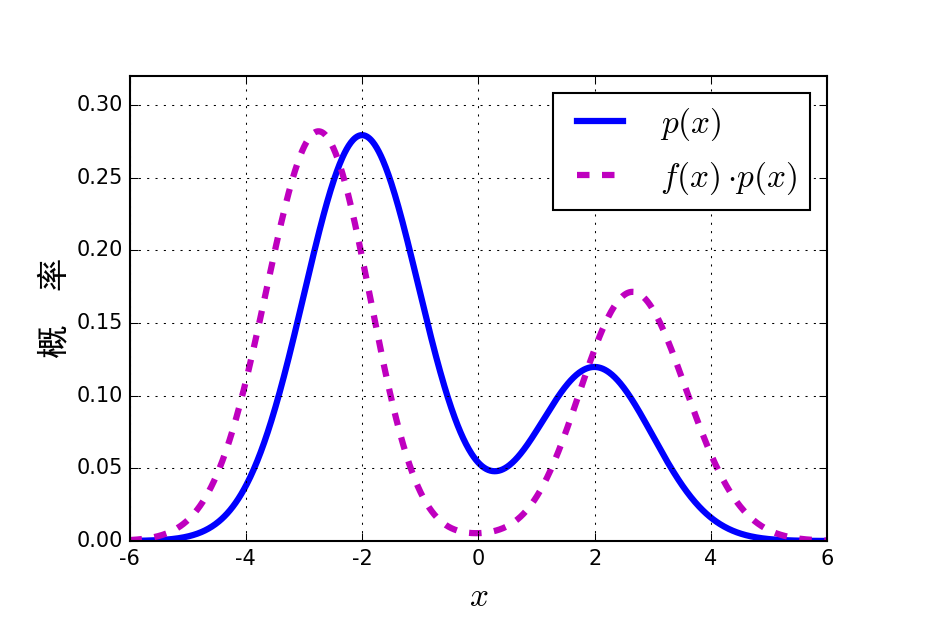
\includegraphics[width=0.5\textwidth]{MCMC/rejectionPxAndfxPx.eps}
\caption{实际分布$p(x)$与$f(x)\cdot p(x)$的函数图像}
\end{figure}

此时,由于$p(x)$并不是一个常见的概率分布,而我们所拥有的一些简单的采样方案基本都是针对于某一类特定的分布而提出的,基于这个原因,这里要想在$p(x)$中采样出$N$个样本并不是一件简单的工作。为此,我们引入舍弃采样来解决在任意分布上采样的问题。

舍弃采样基于这样一个思想:既然我们无法从一个随意的分布$p(x)$上采样,但是可以在一个特殊的分布$q(x)$上采样,比如从高斯分布中采样,那么我们为何不用$q(x)$来逼近$p(x)$呢?为此,我们引入一个分布$q(x)$,称之为提议分布,这个分布需要满足以下条件
\begin{equation}
p(x) < Mq(x),~~~~M<\infty
\end{equation}
式中,$M$是一个定常数,上述约束条件相当于,提议分布$q(x)$与实际分布$p(x)$的比值$p(x)/q(x)$需要在变量$x$的空间$\mathcal{X}$中存在下界$M$。从图像的角度看,提议分布扩大$M$倍后,应该“覆盖”,或者说“包着”实际分布$p(x)$,例如,对于式\eqref{equ:p(x)}的分布$p(x)$,当$M=2.3$且提议分布$q(x)$为
\begin{equation}\label{equ:q(x)}
q(x) = \frac{1}{3\sqrt{2\pi}}\exp\Big(-\frac{(x+1.3)^2}{2\times 3^2}\Big)
\end{equation}
即$q(x)\sim \mathcal{N}(-1.3, 3)$时,实际分布$p(x)$与提议分布$q(x)$的图像如图\ref{img:pxAndqx} 所示

\begin{figure}[htbp]\label{img:pxAndqx}
\centering
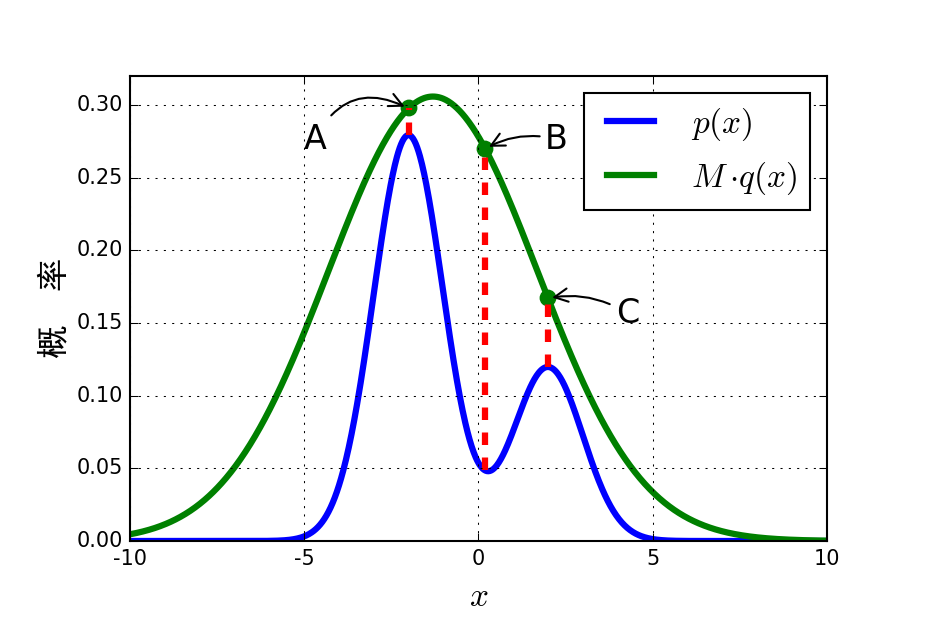
\includegraphics[width=0.5\textwidth]{MCMC/rejectionPxAndQx.eps}
\caption{实际分布$p(x)$与提议分布$q(x)$的函数图像}
\end{figure}

由于提议分布是一个常规的高斯分布,我们有一系列的成熟方法可以在其之上采样出多个样本。假设我们采样得到一个样本后,我们有两种选择:要么接受这个样本,并将这个样本看做是从$p(x)$上采样得到的,要么舍弃这个样本,认为这个样本与$p(x)$采样的样本差距太大,不能看做是$p(x)$的采样样本。

然而,我们什么时候应该接受$q(x)$的样本作为$p(x)$的样本,什么时候又应该拒绝呢?为了刻画这个事件,我们引入了接受概率的概念。假定我们现在已从$q(x)$中采样得到一个样本$x^{(i)}$,则其接受概率$A$我们定义为
\begin{equation}
A = \frac{p(x^{(i)})}{M\cdot q(x^{(i)})}
\end{equation}

计算得到接受概率后,我们以$A$作为接受样本的概率,但在计算机中,没有一种方法直接地描述“以概率A接受样本”这个行为,为了仿真这个行为,我们可以在区间为$[0, 1]$的均匀分布$U(0,1)$上随机生成一个数$u$,若$u<A$则接受样本,否则拒绝。通过这样的方式,我们便可以模拟“以A为概率接受样本”。我们很容易将一个样本推广到$N$个样本的情况,其具体描述如算法\ref{alg:rejection}所示。

\vspace{1em}
\begin{minipage}{0.8\textwidth}\centering
\begin{algorithm}[H]\label{alg:rejection}
 \caption{舍弃采样算法}
  \KwIn{真实分布$p(x)$;提议分布$q(x)$; 采样量$N$}
 \KwOut{$N$个采样样本$\{x^{(i)}\}_{i=1}^N$}
$i=1$\;
\Repeat{$i=N$}
{
采样$x^{(i)}\sim q(x)$,获取随机数$u\sim U(0,1)$,$A = \frac{p(x^{(i)})}{M\cdot q(x^{(i)})}$;\\
\If{$u<A$}
{
接受样本$x^{(i)}$作为$p(x)$的样本,$i += 1$;\\
}
\Else{舍弃样本$x^{(i)}$,$i$保持不变;}
}
\end{algorithm}
\end{minipage}
\vspace{1em}

对于接受概率其定义,一种较为直观的理解是:接受概率$A(x^{(i)})$刻画了$p(x^{(i)})$与$Mq(x^{(i)})$的相似程度。如图\ref{img:pxAndqx}中的A、B、C三点,假设我们可以分别从两个分布中采样得到多个样本,对于$q(x)$而言,采样样本出现在A点附近的概率最大,其次是B点附近,再次是C点附近。然而,对于$p(x)$而言,采样样本出现在B点附近的概率要比出现在C点附近的概率要小,因此,把从$q(x)$中采样得到的样本直接作为$p(x)$的采样样本是不合适的。但由于
\begin{equation}
\frac{p(x_{B\text{附近}})}{M\cdot q(x_{B\text{附近}})} < \frac{p(x_{C\text{附近}})}{M\cdot q(x_{C\text{附近}})}
\end{equation}
B点较小的接受概率使得我们舍弃了$q(x)$采样样本中B点附近大量的样本,C点较大的接受概率使得我们保留了$q(x)$采样样本中C点附近的大量样本,经过舍弃阶段后,我们便可以从$q(x)$的采样样本中筛选出可以刻画$p(x)$性质的样本,因此,舍弃操作可以看做是对样本的纠正。

在$q(x)$定义为式\eqref{equ:q(x)},$p(x)$定义为式\eqref{equ:p(x)}且$M=2.3$的情况下,图\ref{img:hist q(x)}为$q(x)$及采样样本的概率分布直方图,将这些样本经过舍弃后,其分布直方图如图\ref{img:hist P(x)}所示。不难看出,尽管样本是从提议分布$q(x)$中采样得到的,但舍弃采样方法可以很好地逼近原始分布,因此我们可以用筛选后的样本间接地作为$p(x)$的采样样本而不再需要从$p(x)$中直接采样。

\begin{figure}[htbp]
\centering
\subfigure{\label{img:hist q(x)}}\addtocounter{subfigure}{-2}
\subfigure{\subfigure[$q(x)$与样本分布直方图]
			{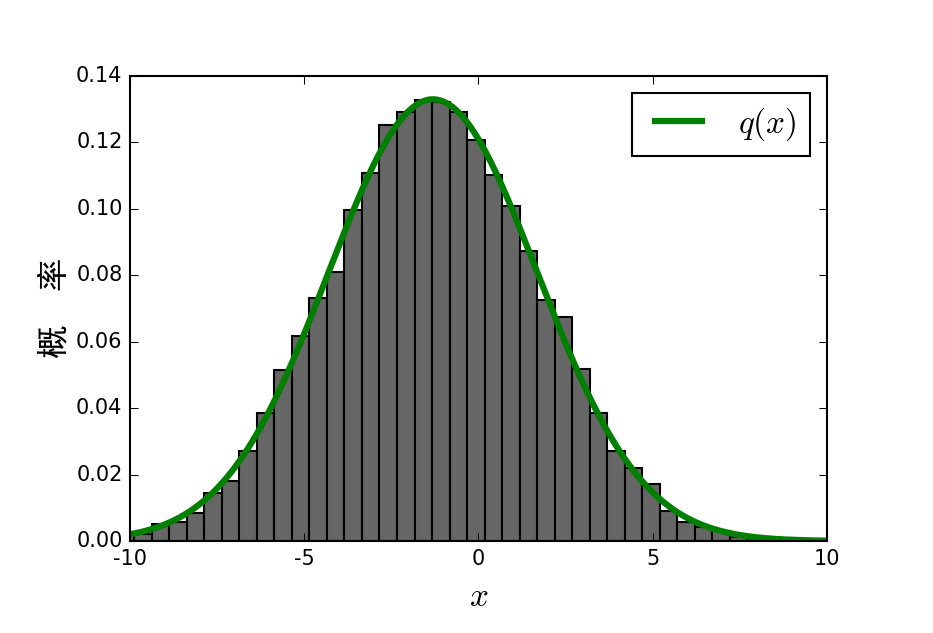
\includegraphics[width=0.4\textwidth]{MCMC/histQx.eps}}}
\subfigure{\label{img:hist P(x)}}\addtocounter{subfigure}{-2}
\subfigure{\subfigure[$p(x)$与筛选后的样本分布直方图]
			{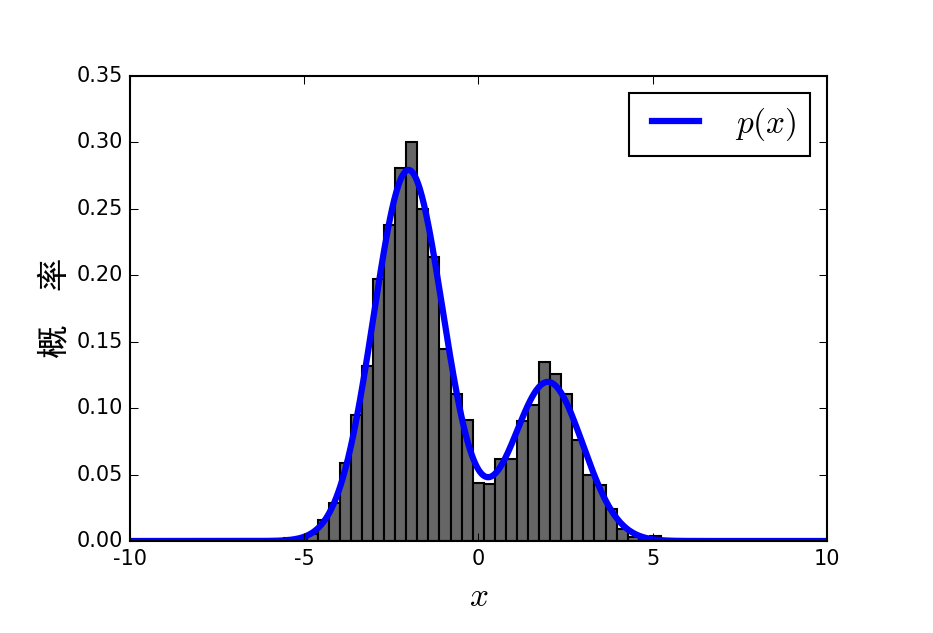
\includegraphics[width=0.4\textwidth]{MCMC/histPx.eps}}}
\caption{舍弃采样的逼近效果}
\vspace{-1em}
\end{figure}

事实上,式\eqref{equ:p(x)}依然过于特殊,其概率密度不过是两个一维高斯分布的线性组合,如果我们将其扩展到二维情形,例如,当真实分布$p(x)$与提议分布$q(x)$分别定义为
\begin{equation}
\begin{split}
p(x) =
& 0.2\cdot \frac{1}{2\pi} \exp\bigg(-\frac{(x+1)^2 + (y+1)^2}{2}\bigg)~ + \\
& 0.1\cdot \frac{1}{2\pi} \exp\bigg(-\frac{(x-3)^2 + (y+3)^2}{2}\bigg)~ +\\
& 0.7\cdot \frac{1}{2\pi} \exp\bigg(-\frac{(x-2)^2 + y^2}{2}\bigg) \\
\end{split}
\end{equation}
\begin{equation}
q(x) = \frac{1}{2\times 2^2 \cdot \pi} \exp\bigg(-\frac{(x-1.5)^2 + y^2}{2\times 2^2}\bigg)
\end{equation}
在$M = 3$时,真实分布与提议分布的图像如图\ref{img:2Dgaussian} 所示

\begin{figure}[htbp]
\centering
\subfigure{\label{img: 2Dgaussian full}}\addtocounter{subfigure}{-2}
\subfigure{\subfigure[全视图]
			{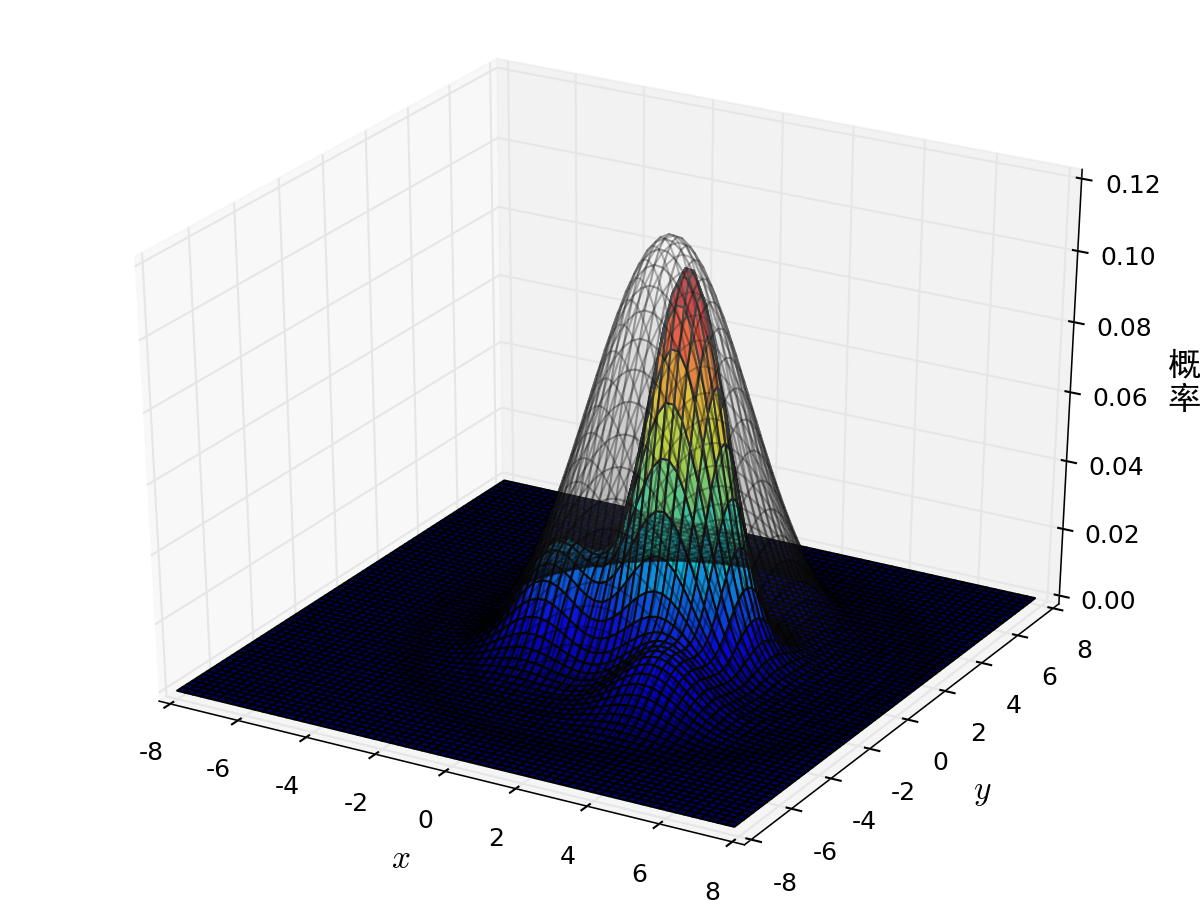
\includegraphics[width=0.4\textwidth]{MCMC/2Dgaussian.eps}}}
\subfigure{\label{img:2Dgaussian part}}\addtocounter{subfigure}{-2}
\subfigure{\subfigure[剖视图]
			{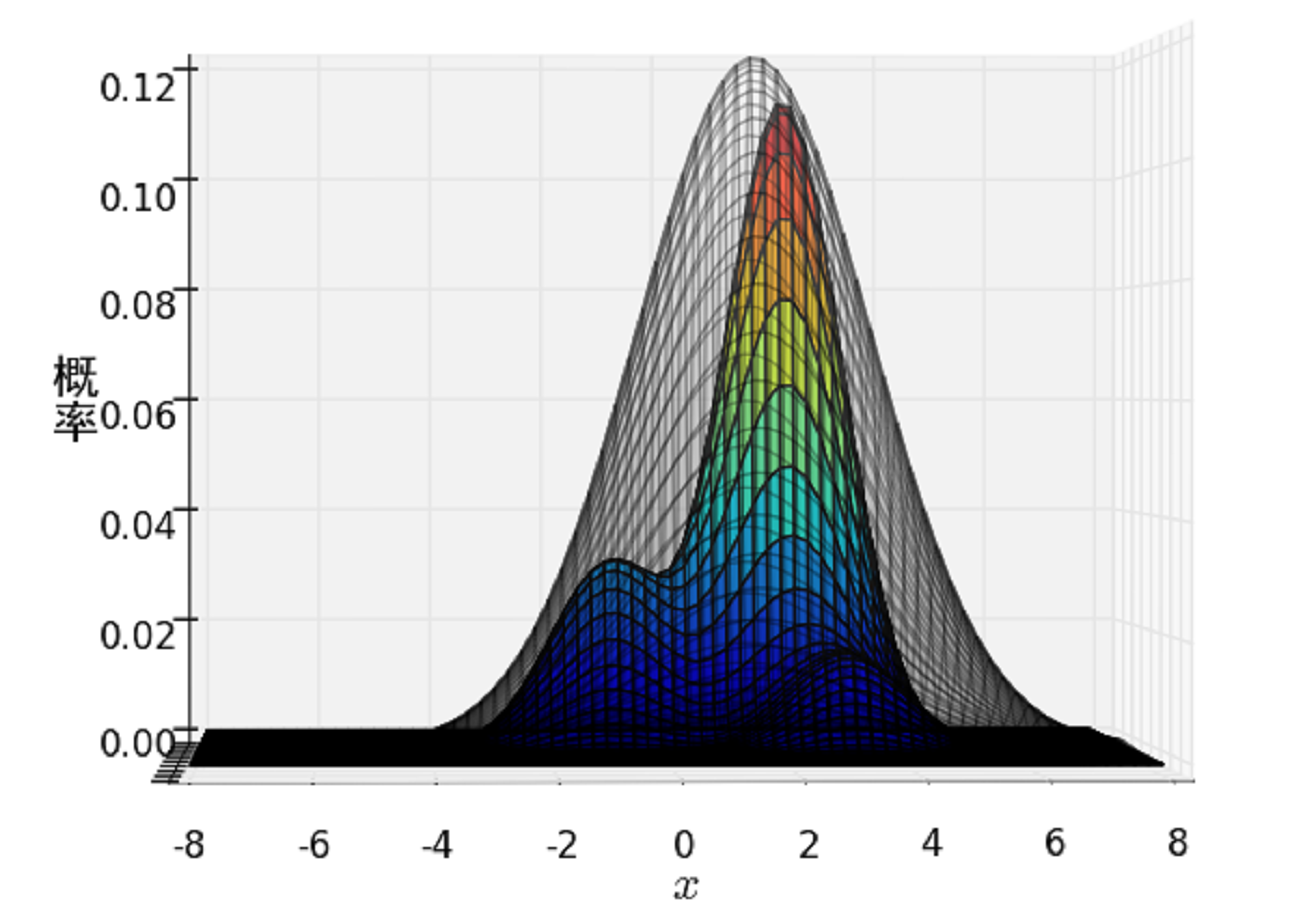
\includegraphics[width=0.4\textwidth]{MCMC/2DgaussianPart.eps}}}
\caption{二维真实分布(彩色)与提议分布(灰色)}
\label{img:2Dgaussian}
\vspace{-1em}
\end{figure}

以上例子都过于简单,实际中我们遇到的一般都是高维的情形,概率密度也更为复杂。这将会导致一个结果,提议分布$q(x)$为了“包住”真实分布$p(x)$,$M$需要取一个很大的值使得$q(x)$可以覆盖掉最凸出的维度。想象这样一种极端的情形,在一个高维度的$p(x)$中,有一个维度是类似于脉冲的尖峰,此时$M$需要取很大才足以覆盖它,但对于剩余的维度而言,$M$可能只需要一个较小的值便可以覆盖掉它们,为了使约束$p(x)< M\cdot q(x)$恒成立,M需要取最大的值,过大的$M$使得接受概率$A = p(x)/Mq(x)$过小,大规模地舍弃样本将使采样速度变慢甚至无法再可以接受的时间内完成采样。究其原因,其最根本的弊端在于$q(x)$必须满足约束$p(x)< M\cdot q(x)$。为了解决这个问题,我们将引入重要性采样,这种方法可以使我们不受约束地选取任意的$q(x)$。


\BiSection{重要性采样}
x回顾章节\ref{section:MCidea}中的讨论,我们为什么要使用舍弃采样?因为蒙特卡罗方法中积分式\eqref{equ:MCintFull}在$p(x)$不是常规的分布形式时难以采样,导致我们无法利用式\eqref{equ:MCintProx}来计算积分。而舍弃采样通过构建一个容易采样的分布$q(x)$,对其采样样本筛选后作为$p(x)$的样本,式\eqref{equ:MCintProx}从而得以进行下去。

式\eqref{equ:MCintProx}之所以能成立,是因为我们利用了点质量函数来逼近概率密度,即
\begin{equation}\label{equ:pn}
p_N(x) = \frac{1}{N}\sum\limits_{i=1}^N \delta_{x^{(i)}}(x)
\end{equation}
式中,$\delta_{x^{(i)}}(x)$为$x^{(i)}$处的脉冲函数。倘若我们不采用这种逼近方式,而采用另外一种,在介绍这种方式之前,我们先引入所谓的重要性权值$w(x)$,即
\begin{equation}
w(x) = \frac{p(x)}{q(x)}
\end{equation}
式中,$q(x)$为任意一个分布。此时,新的逼近方式可以陈述为
\begin{equation}
\hat{p}_N(x) = \sum\limits_{i=1}^N w(x^{(i)})\delta_{x^{(i)}}(x)
\end{equation}
对比式\eqref{equ:pn},我们可以理解为$p_N(x)$中的$1/N$相当于重要性权值恒为$1/N$。引入重要性权值后,积分式\eqref{equ:MCintFull}可以改写为
\begin{equation}
I_f = \int_{-\infty}^{+\infty} f(x)w(x)q(x) dx
\end{equation}
对应的,式\eqref{equ:MCintProx}改写为
\begin{equation}
\hat{I}_f \approx \sum\limits_{i=1}^N f(x^{(i)}) w(x^{(i)})
\end{equation}

如果从另一个角度思考,以上讨论相当于,我们现在有一个目标函数$f(x)$及概率分布$p(x)$,要计算$f(x)$在分布$p(x)$下的期望,由于$p(x)$不是一个常见的分布形式,导致难以利用式\eqref{equ:MCintProx}计算积分, 那么我们构建一个常见的分布形式$q(x)$,将目标函数改写为
\begin{equation}
\hat{f}(x) = \frac{f(x)p(x)}{q(x)} = f(x)w(x)
\end{equation}
则积分式\eqref{equ:MCintFull}变为
\begin{equation}
\hat{I}_f =  \int_{-\infty}^{+\infty} \hat{f}(x)q(x) dx
\end{equation}
此时我们又可以使用类似于式\eqref{equ:MCintProx}的方式来计算积分了。

对比与之前讨论的舍弃采样而言,重要性采样的优点在于$q(x)$不受约束,也不存在舍弃行为,这使得算法效率相对与舍弃采样有所提高。但重要性采样也有其内在缺点,即$q(x)$选取的好坏程度影响着积分的精度,若$q(x)$选取得不好,则需要大量的样本来提高积分精度。刻画$q(x)$好坏的一种准则是最小化$\hat{I}_N f(x)$的方差,即
\begin{equation}
var_{q(x)}\Big[f(x)w(x)\Big] = \mathbb{E}\Big[f^2(x)w^2(x)\Big] - I^2(f)
\end{equation}
由于$I^2(f)$于$q(x)$无关可以摄取,再利用Jensen不等式,有
\begin{equation}
\mathbb{E}\Big[f^2(x)w^2(x)\Big] \geq \mathbb{E}^2\Big[|f(x)|w(x)\Big] = \Big(\int |f(x)|p(x)dx\Big)^2
\end{equation}
因此提议分布可以选取为
\begin{equation}
q(x) = \frac{|f(x)|p(x)}{\int |f(x)|p(x)dx}
\end{equation}
由于分母只是一个归一化常数可以不管,我们现在要做的是在$|f(x)|p(x)$中采样,这看起来似乎没有什么用,实际上也确实没有什么用,毕竟$|f(x)|p(x)$并不似一个容易采样的函数。但它启示我们一点,如果$p(x)$的样本落在的重要域可以使得$|f(x)|p(x)$取值较大,那么采样效率将会非常高,这也是重要性采样的命名来源。

无论是舍弃采样还是重要性采样都是独立采样,即样本之间是独立的,从而采样效率较低。为了提高采样效率,我们可以使用关联采样,即样本之间存在关联,构建样本之间的关联性所要用到的便是著名的马尔可夫链。


\BiSection{马尔可夫链}
在正式引入马尔可夫链之前,我们打算先从一个随机游走的例子入手。想象一个正方形区域内,在某一点放入N个粒子,这些例子随机地朝着各个方向游走。对于每一个粒子而言,每一次游走的步长是相等的,只是角度随机选择。当粒子移动到正方形的边界是,它将被反弹回正方形区域内。直觉上的想象,经过漫长的时间,粒子将漫布在整个正方形区域内。如图\ref{img:randomWalk} 所示是两个随机游走的例子,其中蓝色的初始状态在中心附近,绿色的初始状态在左下角。
\begin{figure}[htbp]
\centering
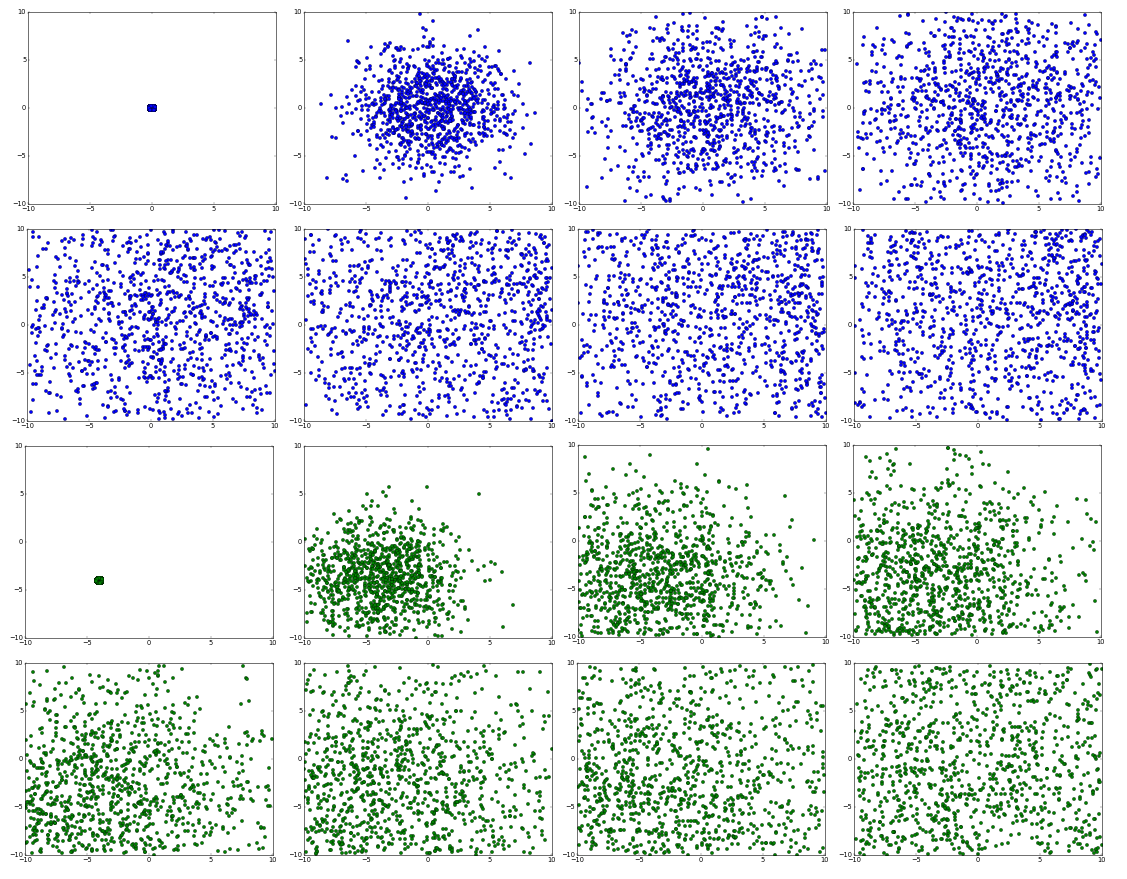
\includegraphics[width=0.5\textwidth]{MCMC/randomWalk.eps}
\caption{两个随机游走的例子}\label{img:randomWalk}
\end{figure}

这个例子类似于布朗运动,有趣的现象是,起始位置的选取并不会影响最终结果---粒子将呈均匀分布。正如一锅未加盐的汤,无论盐从哪个位置撒下,最终整锅汤的咸淡是均匀的。对于某个特定的粒子而言,追中它的轨迹是无意义的,从宏观上看,粒子下一步处于哪个位置与之前的位置无关,只与它当前的位置有关,因为它是经过怎样的路径到达当前的状态对下一步移动到哪里起不到任何作用。

马尔可夫链意识基于同一个原理,假设我们的变量$x$可取得状态有$s$个,那么集合$S = \{x_1, x_2, x_s\}$被称为状态空间,马尔可夫链刻画的是变量$x$在状态空间$S$中各个状态之间迁移的轨迹。类似于随机游走的例子,马尔可夫链的下一个状态与之前的状态无关,之与当前的状态有关,即
\begin{equation}
p(x^{(i+1)} | x^{(i)} \cdots x^{(1)}) = p(x^{(i+1)} | x^{(i)})
\end{equation}
这个性质也被称为马尔科夫性质。对于给定的系统,我们定义某个状态转移到另一个状态的概率为转移概率,即
\begin{equation}
p(x^{(i+1)} | x^{(i)}) = T(x^{(i)} \rightarrow x^{(i+1)})
\end{equation}

如图\ref{img:MCfigure} 中的系统,状态空间为$\{A, B, C\}$,由图中的参数我们容易算得转移矩阵$\mathcal{T}$
\begin{figure}[htbp]
\centering
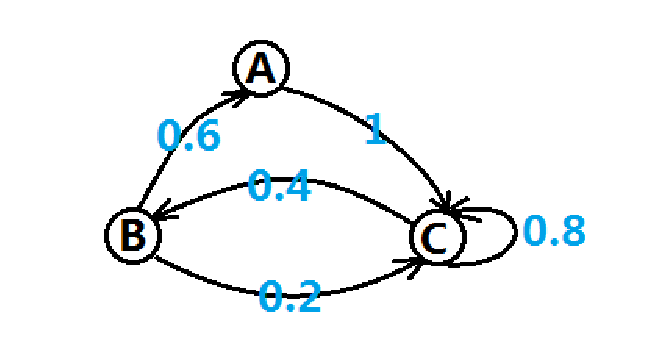
\includegraphics[width=0.5\textwidth]{MCMC/MCfigure.eps}
\caption{马尔科夫链}\label{img:MCfigure}
\end{figure}
\begin{equation}
\mathcal{T} = \left[
\begin{array}{ccc}
T(A\rightarrow A)~~ & T(A\rightarrow B)~~ & T(A\rightarrow C)\\
T(B\rightarrow A)~~ & T(B\rightarrow B)~~ & T(B\rightarrow C)\\
T(C\rightarrow A)~~ & T(C\rightarrow B)~~ & T(C\rightarrow C)\\
\end{array}
\right]
=\left[
\begin{array}{ccc}
0 & 0 & 1\\
0.6 &0 & 0.4\\
0 & 0.2 & 0.8
\end{array}
\right]
\end{equation}

倘若我们为A、B、C赋予一些实际意义,我们令A代表下雨,B代表多云,C代表晴天,又假设今天的天气为晴天,现在我们要估计10天后的天气状况。首先,我们可以很容易地将今天的天气描述为一个向量
\begin{equation}
x = [1~~0~~0]
\end{equation}
为了计算10天后的天气,用$x$乘以10次转移矩阵后将得到10天后的天气状况,即
\begin{equation}
[1~~0~~0] \times
\left[
\begin{array}{ccc}
0 & 0 & 1\\
0.6 &0 & 0.4\\
0 & 0.2 & 0.8
\end{array}
\right]^{10}
=[0.091~~0.151~~0.758]
\end{equation}
也就是说,10天后下雨的概率为0.091,多云的概率为0.151,晴天的概率为0.758。倘若我们假设今天的天气为多云,利用同样的方法,我们可以计算得10天后的天气状况为
\begin{equation}
[0~~1~~0] \times
\left[
\begin{array}{ccc}
0 & 0 & 1\\
0.6 &0 & 0.4\\
0 & 0.2 & 0.8
\end{array}
\right]^{10}
=[0.091~~0.151~~0.758]
\end{equation}
我们发现,不管今天是雨天开始多云,计算得到10天后的天气情况是十分接近的(这里完全一样是因为我们舍去了尾部小数),如果读者有兴趣的话可以验证初始状态为晴天是得到的结果也是一样的。也就是说,不管今天的天气如何,对10天后的天气均无影响。

之所以出现这种现象是因为马尔可夫链在第十个周期时已经进入一个我们称之为平稳的状态。类似于之前的随机游走,当经过足够长的时间后,系统的状态与初始状态再无关联,至于系统的结构(也就是转移矩阵)有关。但并不是所有的转移矩阵都能达到平稳,在这里,我们并不打算深入讨论,只给出结论定理
\begin{theorem}\label{theo:MC}
如果一个马尔科夫链是各态遍历的,那么存在一个时间$t_s$,当$t>t_s$时,马尔可夫链到达一个平稳分布$x^*$,其中$x^*$满足
\begin{equation}
x^* = x^* \mathcal{T}
\end{equation}
\end{theorem}
所谓各态遍历,即要求马尔可夫链是不可约且非周期的,所谓不可约,即所有状态都是有关联的,从某个状态出发,不存在无法到达的状态,所谓非周期,即马尔可夫链不会陷入某几个状态间循环,满足上述两个条件的马尔可夫链我们称它是各态遍历的。

利用马尔可夫链的这个性质,我们就可以实现关联采样。由于初始状态与稳态无关,我们可以随机设置,经过多次随机游走,进入稳态后得到的状态便可以作为一个样本。以上讨论均基于一个前提,即转移矩阵是已知的。然而,实际中,我们并不知道转移矩阵的数值。例如,我们并不知道由晴天转移到多云的概率是0.2,这个数值是我们捏造的。但是一旦转移矩阵知道了,采样问题便迎刃而解,目前成熟的马尔可夫链蒙特卡罗方法整体框架都是类似的,不同的地方往往在于转移矩阵的构造上。

\BiSection{Metropolis-Hastings算法}
x与舍弃采样类似,Metropolis-Hastings算法(以下简称MH算法)也存在一个提议分布,这个提议分布定义为$q(x^*|x)$,不同的是,舍弃采样中的提议分布受一个强约束,即$p(x) < Mq(x)$,而MH算法中的提议分布只需要满足$q(x^*|x)>0$即可,显然这个约束相当于没有约束,因为概率论三大公理的第一条就使这个约束成立了。另一个不同点在于,MH算法中的提议分布其意义为:在当前状态$x$下,由提议分布$q(x^*|x)$产生一个试探性状态$x^*$,随后根据接受概率决定是否转移到新状态$x^*$上,这里,接受概率定义为
\begin{equation}\label{equ:MHaccept}
A = \frac{p(x^*)\cdot q(x|x^*)}{p(x)\cdot q(x^*|x)}
\end{equation}
此时,若接受概率$A > 1$,则接受这个新状态,否则,以概率$A$接受新状态。若接受了这个新状态$x^*$,则状态从$x$转移到$x^*$处,并在$x^*$处的提议分布$q(x^{**}|x^*)$产生一个新的试探状态$x^{**}$,如此反复循环,若不接受这个状态$x^*$,则状态仍然停留$x$处。

需要注意的一点是,在MH采样中,提议分布$q(x^*|x)$是对着状态$x$的变动而变动的,例如,如果我们将提议分布$q(x^*|x)$设计成一个在以$x$为中心,以2为方差的高斯分布,即$q(x*|x)\sim \mathcal{N}(x, 2)$,那么如图\ref{img:diffStateDiffQx}所示,在$x^{(1)}$状态和$x^{(2)}$状态下的提议分布是不同的。

\begin{figure}[htbp]
\centering
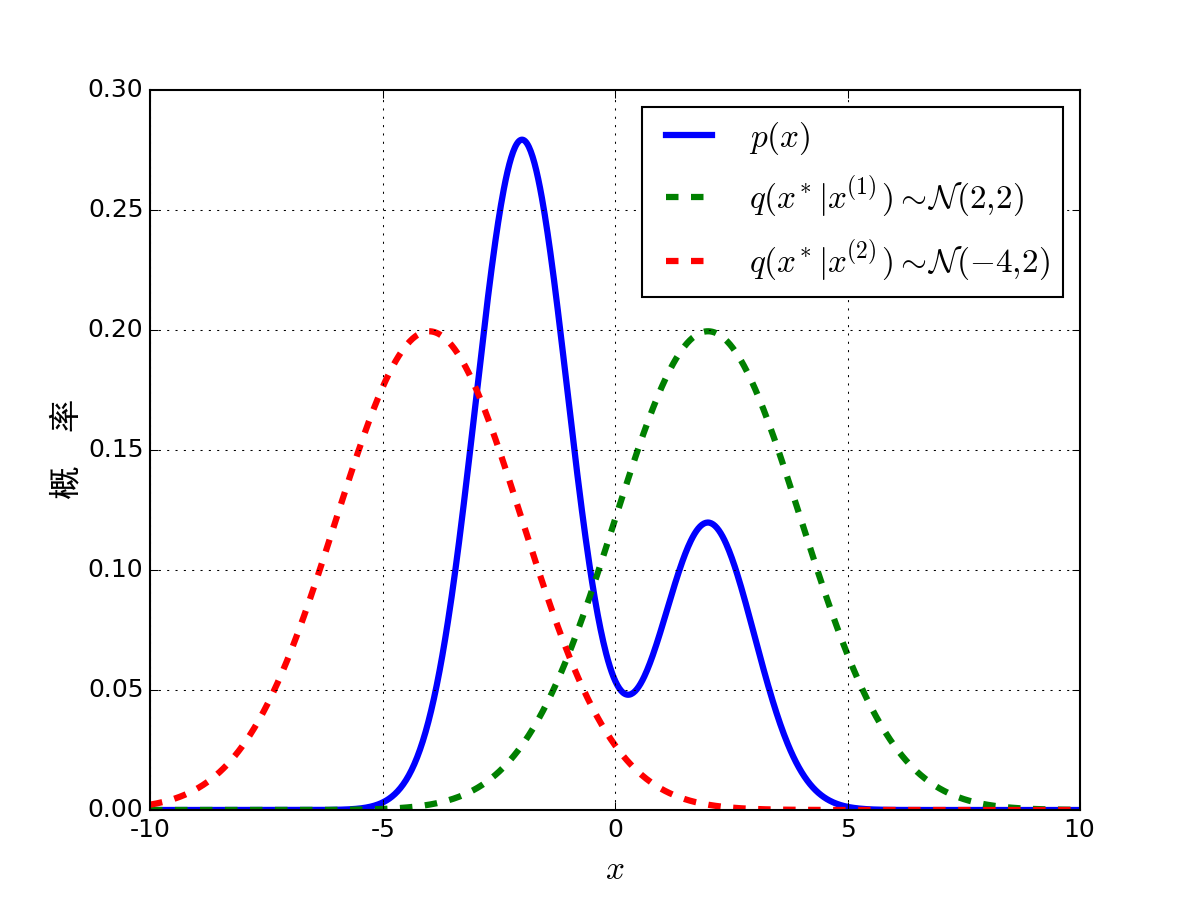
\includegraphics[width=0.5\textwidth]{MCMC/diffStateDiffQx.eps}
\caption{不同状态下的提议分布}\label{img:diffStateDiffQx}
\end{figure}


综合以上的讨论,MH算法可以描述为算法\ref{alg:MH} 中的过程。

\vspace{1em}
\begin{minipage}{0.8\textwidth}\centering
\begin{algorithm}[H]\label{alg:MH}
 \caption{Metropolis-Hastings算法}
  \KwIn{真实分布$p(x)$;提议分布$q(x^*|x)$; 游走次数$N$}
 \KwOut{$1$个采样样本$x^{(N)}$}
设置初始状态$x^{(0)}$,$i=0$\;
\Repeat{$i=N$}
{
采样$x^*\sim q(x^*|x^{(i)})$,获取随机数$u\sim U(0,1)$;\\
计算接受概率$A = \frac{p(x^*)\cdot q(x|x^*)}{p(x)q(x^*|x)}$\\
\If{$u<A$}
{
$x^{(i+1)} = x^*$;\\
}
\Else{$x^{(i+1)} = x^{(i)}$}
}
返回$x^{(N)}$
\end{algorithm}
\end{minipage}
\vspace{1em}

相比于舍弃采样,舍弃采样的拒绝是直接抛弃样本,而MH采样的拒绝是让样本停留在当前状态。另一个不同点在于,算法\ref{alg:MH}描述的是采样出一个样本的过程,是一个随机游走的过程,而算法\ref{alg:rejection}描述的是采样出$N$个样本的过程。尽管算法\ref{alg:MH}只能采样出一个样本,但是我们也可以很容易将其扩展成为残阳$N$个样本的算法。另外,由于各个样本的随机游走是独立的,不存在线程安全问题,因此算法\ref{alg:MH}可以很容易设计成为并行算法。

正如我们提到的,如果我们使用一个形式为$q(x*|x)\sim \mathcal{N}(x, 2)$的提议分布区采样1000个式\eqref{equ:p(x)}中实际分布$p(x)$的样本,对于不同的游走次数$N$,其结果如图\ref{img:MH} 所示

\begin{figure}[htbp]
\centering
\subfigure{}\addtocounter{subfigure}{-2}
\subfigure{\subfigure[$N=10$]
			{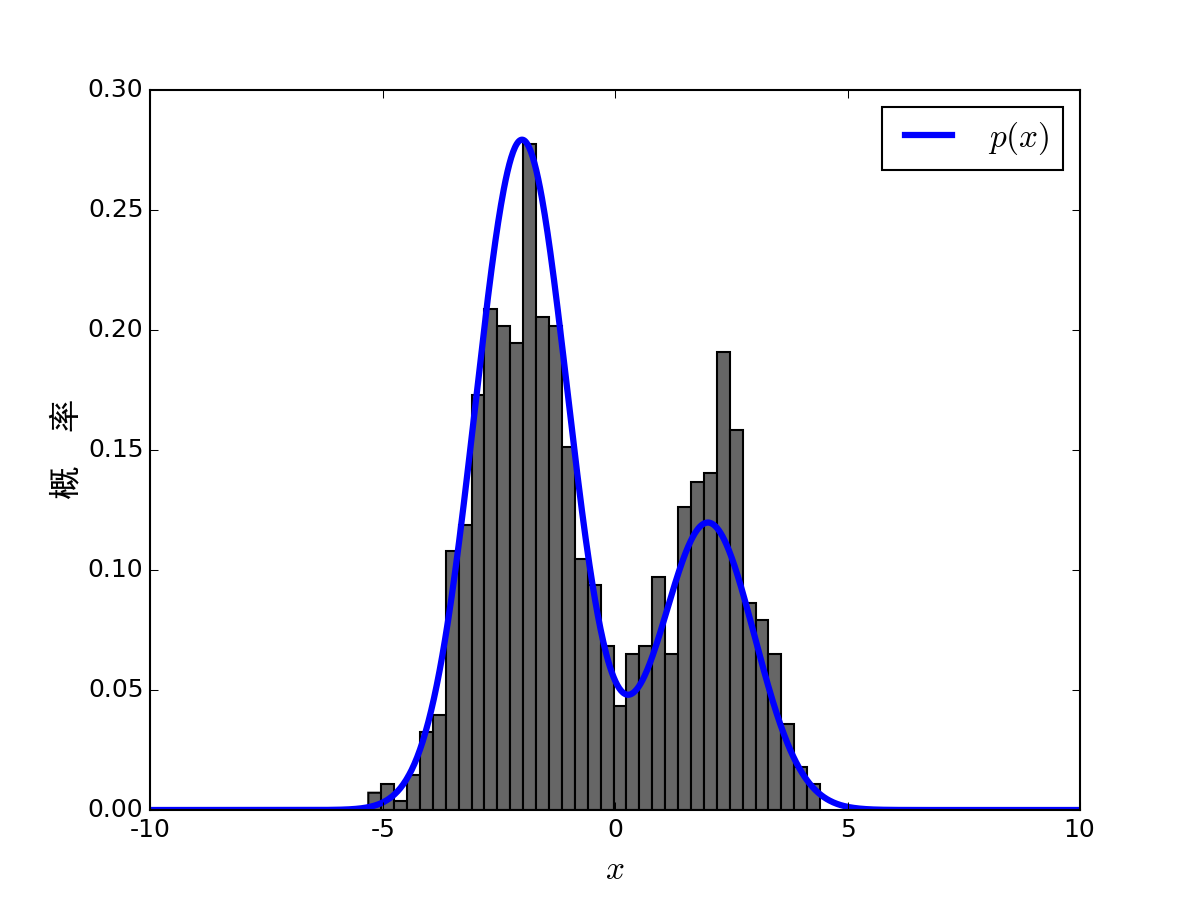
\includegraphics[width=0.4\textwidth]{MCMC/MH10.eps}}}
\subfigure{}\addtocounter{subfigure}{-2}
\subfigure{\subfigure[$N=100$]
			{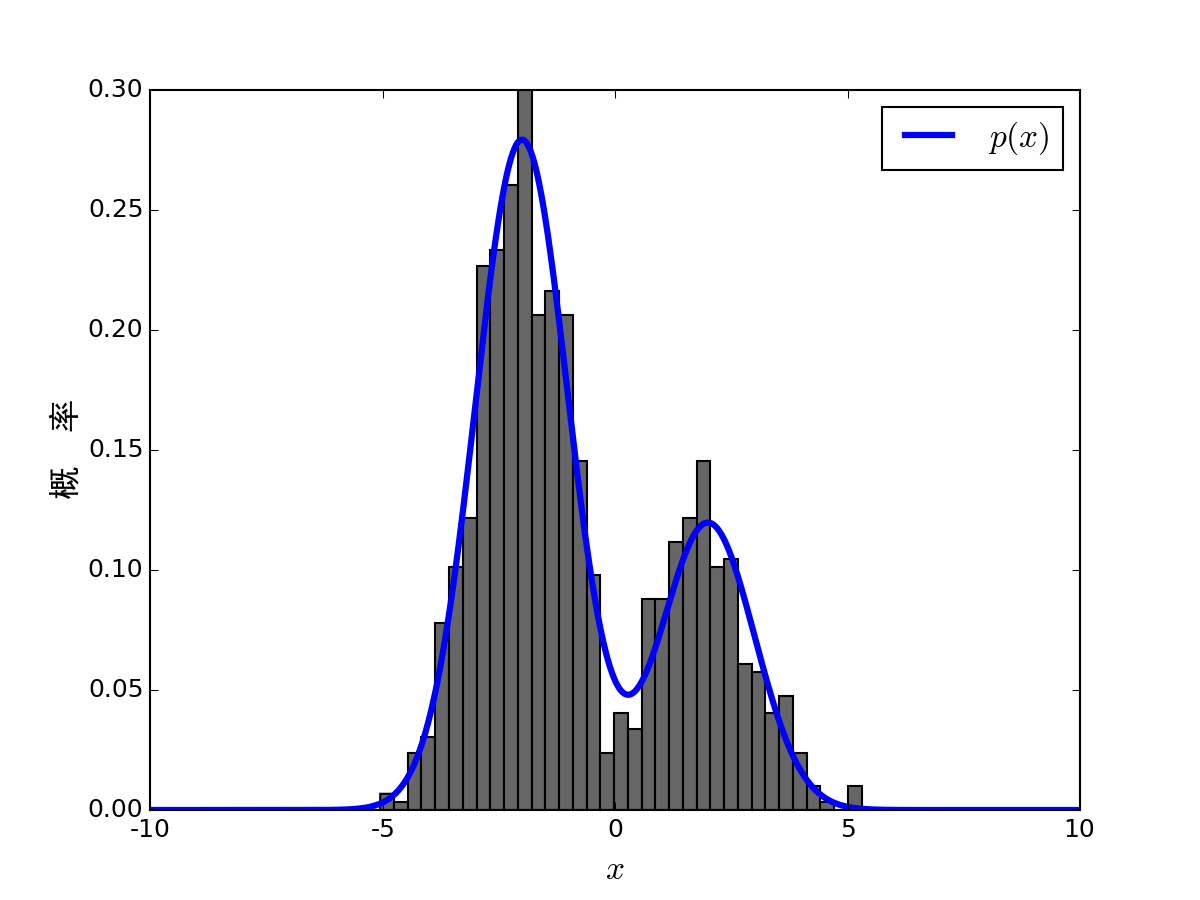
\includegraphics[width=0.4\textwidth]{MCMC/MH100.eps}}}
\subfigure{}\addtocounter{subfigure}{-2}
\subfigure{\subfigure[$N=1000$]
			{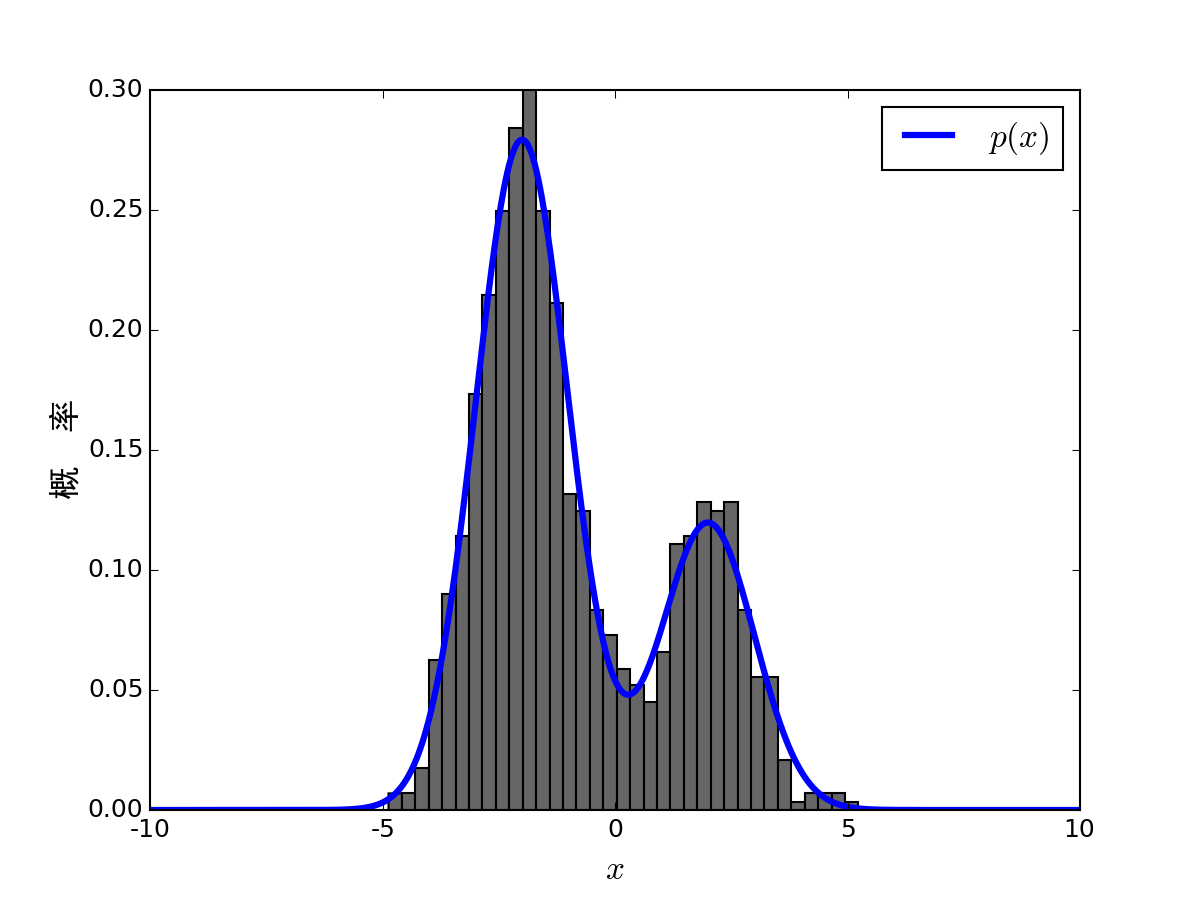
\includegraphics[width=0.4\textwidth]{MCMC/MH1000.eps}}}
			\subfigure{}\addtocounter{subfigure}{-2}
\subfigure{\subfigure[$N=100$]
			{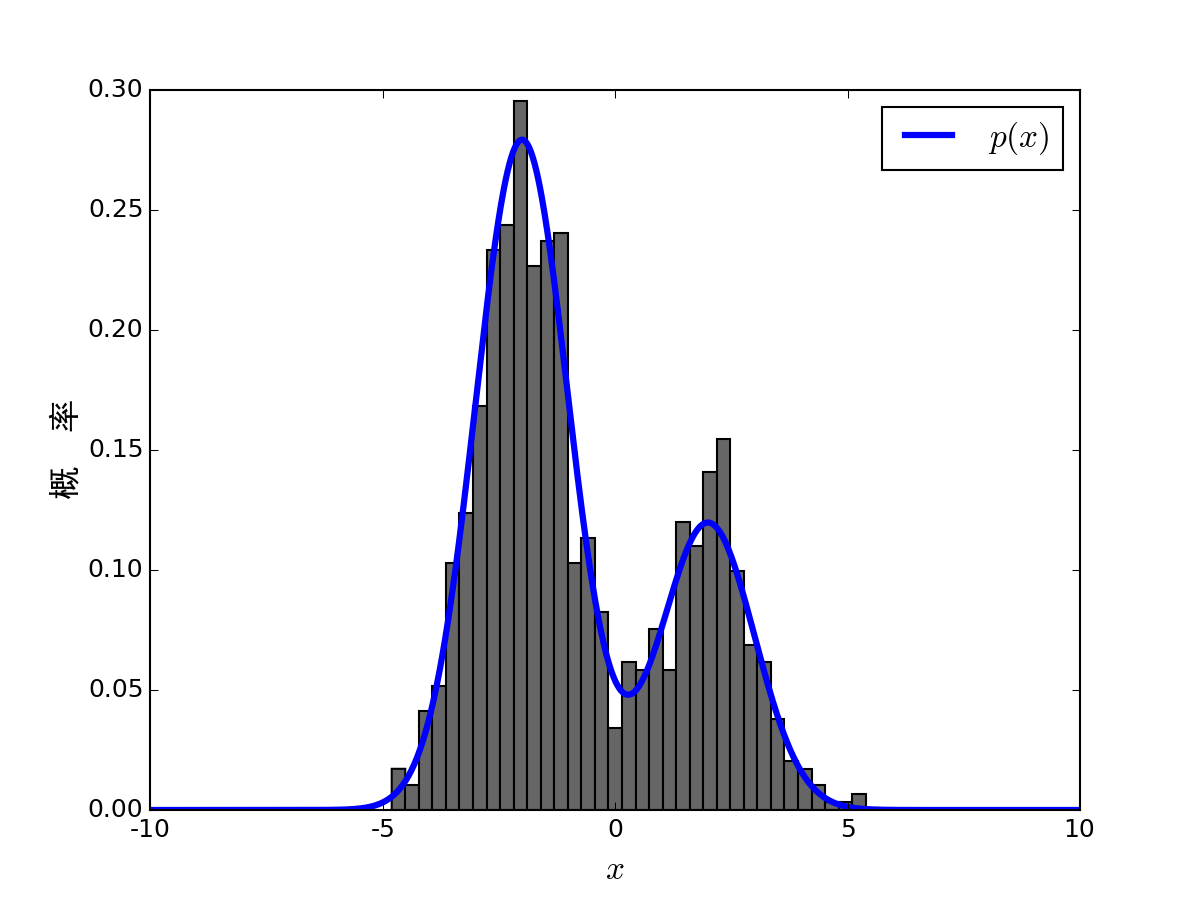
\includegraphics[width=0.4\textwidth]{MCMC/MH5000.eps}}}
\caption{不同游走次数下的样本分布直方图}
\label{img:MH}
\vspace{-1em}
\end{figure}

从图中我们不难发现,在游走次数$N=10$是,逼近效果并不完美,随着$N$的增大,当$N=100$时,采样结果已经能很好地刻画实际分布了。此时,$N$再增大(比如1000或5000)已经差别不大了。从随机游走的角度上看,可以理解为,$N=100$时就已经进入平稳分布了,再继续游走下去并没有太大意义。

MH采样可以认为是很多MCMC方法的模板,其他的MCMC方法大多都是MH算法的特例。之所以会从MH算法中衍生出这么多的分支是因为MH有其自身的局限性。首先,我们难以估计状态是否进入平稳状态,即游走次数$N$难以确定。其次,MH算法在高维问题中的效果并不好,因为高维空间的地形复杂,MH算法一不小心就会落入一个周围状态的接受概率都很小的区域,这将导致试探状态不断地被否决,从而长时间留滞在该点附近。接受概率的存在,使得游走效率低下,而Gibbs采样时MH采样的一个特例,这种方法不存在接受概率,或者说接受概率为1,因此每一次游走都将得到一个新的状态,这个特性将大大地加快收敛速度。

\BiSection{Gibbs采样}
xGibbs采样又称为热浴方法或“Glaber动力学”,常用于解决高维分布中的采样问题。假设我们有一个$d$维向量$x$,并且知道任一分量的条件概率分布形式
\begin{equation}
p(x_j|x_{-j}) \triangleq p(x_j|x_1, \cdots, x_{j-1}, x_{j+1}, \cdots x_d)
\end{equation}
则我们构建提议分布
\begin{equation}\label{equ:GibbsQx}
q(x^*|x) = \left\{
\begin{array}{cc}
p(x^*_j|x_{-j}) & \text{若} x^*_{-j} = x_{-j}\\
0 & \text{其他}
\end{array}
\right.
\end{equation}

由于Gibbs采样是MH采样的特例,而MH采样的接受概率公式\eqref{equ:MHaccept}又可以描述为
\begin{equation}\label{equ:MHaccept2}
A = \min\Big\{1, \frac{p(x^*)\cdot q(x|x^*)}{p(x)\cdot q(x^*|x)} \Big\}
\end{equation}
将式\eqref{equ:GibbsQx}代入式\eqref{equ:MHaccept2},并利用$x^*_{-j} = x_{-j}$性质以及贝叶斯公式,有
\begin{equation}\label{equ:GibbsAccept}
\begin{split}
A &= \min\bigg\{1, \frac{p(x^*)\cdot p(x_j|x^*_{-j})}{p(x)\cdot p(x^*_j|x_{-j})} \bigg\}\\
&=\min\bigg\{1, \frac{p(x^*)\cdot p(x_j|x_{-j})}{p(x)\cdot p(x^*_j|x^*_{-j})} \bigg\}\\
&=\min\bigg\{1, \frac{p(x_{-j})}{p(x^*_{-j})} \bigg\}\\
&=1
\end{split}
\end{equation}

由式\eqref{equ:GibbsAccept}我们不难得出结论,Gibbs的接受概率恒为1,亦即在Gibbs采样中,我们不存在丢弃样本或状态停滞的行为,每一次都会转移到一个新的状态上,这显然会加快算法的收敛速度。

以上内容未免过于晦涩,为了方便大家理解,我们将再次阐述Gibbs采样的原理。首先,Gibbs采样要基于一个大前提---真实分布$p(x)$在各个维度的条件概率分布是已知的,即$p(x_j|x_1,\cdots, x_{j-1}, x_{j+1}, \cdots, x_d)$已知。如果这个条件概率分布是未知的,则使用Gibbs采样不是一个恰当的策略,应为Gibbs采样的提议分布是基于这个条件概率分布之上构建出来的。式\eqref{equ:GibbsQx}定义的提议分布,其含义为:固定$x_1,\cdots, x_{j-1}, x_{j+1}, \cdots, x_d$这$d-1$个维度的状态不变,单独处理$d$个维度中的一个,即$x_j$。如果将Gibbs采样试想成为一只章鱼,那么每次它都只迈出一只脚,当这只脚固定后,再迈出剩下的另一只脚,因此,Gibbs采样的算法描述如算法所示。

\vspace{1em}
\begin{minipage}{0.8\textwidth}\centering
\begin{algorithm}[H]\label{alg:Gibbs}
 \caption{Gibbs采样算法}
  \KwIn{各个维度的条件分布$p(x_j|x_{-j})$; 游走次数$N$}
 \KwOut{$1$个采样样本$x^{(N)}$}
设置初始状态$x^{(0)}$,$i=0$\;
\Repeat{$i=N$}
{
采样出第1个维度$x_1^{(i+1)} \sim p(x_1|x_2^{(i)}, x_3^{(i)}, \cdots, x_d^{(i)})$\\
采样出第2个维度$x_2^{(i+1)} \sim p(x_2|x_1^{(i+1)}, x_3^{(i)}, \cdots, x_d^{(i)})$\\
~~~~~~~~~~~~~~~~~~~~~~~~~~~~~~~~~~~~~~~~$\vdots$\\
采样出第$j$个维度$x_j^{(i+1)} \sim p(x_j|x_1^{(i+1)},  \cdots, x_{j-1}^{(i+1)}, x_{j+1}^{(i)}, x_d^{(i)})$\\
~~~~~~~~~~~~~~~~~~~~~~~~~~~~~~~~~~~~~~~~$\vdots$\\
采样出第$d$个维度$x_d^{(i+1)} \sim p(x_d|x_1^{(i+1)}, x_2^{(i+1)}, \cdots, x_{d-1}^{(i+1)})$\\
}
返回$x^{(N)}$
\end{algorithm}
\end{minipage}
\vspace{1em}

至此,MCMC的大体内容已讨论完毕,让我们回到第\ref{chapter:RBM}章遗留的问题。第\ref{chapter:RBM}章中,式\eqref{expectFunc},即
\begin{equation}
 \frac{\partial\ln\mathcal{L}_{\hat{v}} }{\partial\theta} =  
 -\mathbb{E}_{p(h|\hat{v})}\bigg[ \frac{\partial E(\hat{v}, h)}{\partial \theta} \bigg]
 + \mathbb{E}_{p(v, h)}\bigg[\frac{\partial E(v, h)}{\partial \theta}\bigg]
\end{equation}
我们说,式中的第一项期望是容易处理的,而第二项却难以处理,因为如果我们采用穷举的方法解决这个问题,这将会是一个$O(2^{n_v+n_h})$复杂度的运算,但采用MCMC的方法就很好处理。由于目前我们需要解决的问题是$\frac{\partial E(v, h)}{\partial \theta}$在分布$p(v, h)$下的期望,根据式\eqref{eq:RBMenergy}中对能量函数$E(v,h)$的定义,偏导数非常容易求取。如果我们能在$p(v, h)$中采样出多个样本,那么这个问题便迎刃而解。但采样$p(v,h)$是一件困难的事,幸运的是,我们知道$p(v,h)$的条件概率$p(v|h)$以及$p(h|v)$,即式\eqref{p(h|v)}和式\eqref{p(v|h)},因此我们完全可以通过Gibbs采样,经过多次状态转移后采样出一个样本,再以同样的方法采样出多个样本,利用这多个样本,加以式\eqref{equ:MCintProx},便可以算出期望值,整个问题便解决了。

\BiSection{对比离差}
x尽管第\ref{chapter:RBM}章遗留的问题可以通过Gibbs采样解决,但事实上,正如我们前面提及到的,马尔可夫链进入平稳分布的时间难以确定。我们知道,马尔可夫链的初始状态对平稳分布在性质上是没有影响的,但是不同的初始状态会影响进入平稳分布的时间。就如同往汤里加盐,在不同的位置撒下并不会影响最后的咸淡,但会影响盐在水中的扩散速度,Gibbs采样也同理,不同的初始值对收敛速度有影响。如果初始值随机设置,则模型的训练速度十分缓慢。Hinton提出了一种名为对比离差\citeup{onCDlearn}(Contrastive Divergence,简写为CD)的方法,其中心思想是:既然数据出现了,那么说明这个数据是接近于平稳分布的,因此我们令初始值为该数据样本,进行吉布斯采样,所以,对比离差算法如算法\ref{alg:CD-k}所示。

\vspace{1em}
\begin{minipage}{0.8\textwidth}\centering
\begin{algorithm}[H]\label{alg:CD-k}
 \caption{CD-k算法}
  \KwIn{条件分布$p(h|v)$和$p(v|h)$; 迭代次数$k$}
 \KwOut{$1$个采样样本$v^{(k)}$}
设置初始状态$x^{(0)}=data$,$i=0$\;
\Repeat{$i=k$}
{
采样出$h^{(i)} \sim P(h|v^{(i)})$\\
采样出$v^{(i+1)} \sim P(v|h^{(i)})$\\
}
返回$v^{(k)}$
\end{algorithm}
\end{minipage}
\vspace{1em}

算法\ref{alg:CD-k}也被称为CD-k算法,随着k的增大,采样得到的样本越接近于模型的平稳分布,但在实验中,$k=1$的时候已经能获得很不错的结果,因此我们往往令$k=1$。而得到最终的采样样本$v^{(k)}$后,对数似然的梯度近似为
\begin{equation}
\frac{\partial\ln P(v)}{\partial w_{i, j}} \approx
 P(h_i = 1 | v^{(0)})v_j^{(0)} - P(h_i = 1 | v^{(k)})v_j^{(k)}
 \label{equ:MAMAMA}
\end{equation}

\begin{equation}
\frac{\partial\ln P(v)}{\partial b_{vi}} \approx
v_j^{(0)} - v_j^{(k)}
\label{equ:MBMBMB}
\end{equation}

\begin{equation}
\frac{\partial\ln P(v)}{\partial b_{i}} \approx
 P(h_i = 1 | v^{(0)}) - P(h_i = 1 | v^{(k)})
 \label{equ:MCMCMC}
\end{equation}

CD-k算法可以认为是利用
\begin{equation}
CD_k = -\sum\limits_{h}P(h|v^{(0)})\frac{\partial E(v^{(0)} , h)}{\partial \theta} + \sum\limits_{h}P(h|v^{(k)})\frac{\partial E(v^{(k)} , h)}{\partial \theta}
\end{equation}
来近似\citeup{approximations}
\begin{equation}
\frac{\partial P(v)}{\partial \theta} = -\sum\limits_{h}P(h|v^{(0)})\frac{\partial E(v^{(0)} , h)}{\partial \theta} + \sum\limits_{v, h}P(v, h)\frac{\partial E(v , h)}{\partial \theta}
\end{equation}
利用CD-k,可以很高效地求得参数的增量$\Delta W$、$\Delta b_v$以及$\Delta b_h$,从而训练受限玻尔兹曼机来刻画数据的分布。


\BiSection{本章小结}
x本章从蒙特卡罗的核心思想说起,引入舍弃采样,由于舍弃采样的提议分布受到一个约束,为此我们又引入重要性采样。无论是重要性采样或是舍弃采样,都属于非关联采样,因此我们引入马尔可夫链,得到一个关联采样方法,即MH采样。MH采样在高维空间中效果并不好,且存在接受概率使算法效率较低,为此我们引入用于解决高维问题且不存在接受概率的Gibbs采样,通过Gibbs采样可以第\ref{chapter:RBM}章的期望问题,但Gibbs的收敛速度依赖于初始值的设定,为了选取一个较好的初始值,也为了加快算法的收敛速度,我们引入了对比离差方法。通过对比离差,可以高效的解决第\ref{chapter:RBM}章中的期望问题。事实上,马尔可夫链蒙特卡罗方法其潜力并不仅局限于此,这套方法在机器学习中还有更为广泛的应用,然而我们并没有涉及。至此,受限玻尔兹曼机的内容讨论完毕,通过一个训练好的RBM,就可以刻画数据的分布。但目前的讨论并没有进入到核心内容,我们仍没有讨论识别,或者说分类问题。在第\ref{chapter:DBN}章中,我们将介绍如何用多个RBM作为砖块垒出一个深度置信网络,并用这个网络进行图像识别。










\BiChapter{深度置信网络}{DBN}\label{chapter:DBN}
深度置信网络是由Hinton于2006年提出的一种深度全连接神经网络,全连接的深度神经网络的训练是及其困难的,然而在深度置信网络中,我们采用网络的逐层训练,随后对网络参数的微调,这种策略使得我们可以容易地训练多层神经网络。由于深度置信网络本质是一种传统神经网络的推广,在本章中,我们将从传统神经网络说起,介绍其训练方法,逐步将其推广到深度置信网络。
\BiSection{神经网络组成及表达能力}
x一个神经网络往往由多层神经元组成,神经元作为网络的基本单元,在给定恰当的激活函数和权值的前提下,只要这个网络足够庞大,足以容纳较多的神经元,那么这个网络可以表达任何一个连续函数\citeup{barron1993universal},当然这只是一个理论上成立的理想情况,实际工程中,我们没有办法利用神经网络来描述所有的函数,但是这个定理能使我们对神经网络的表达能力充满信心。
\BiSubsection{神经元}
x一个神经元如图\ref{img:NNnode_cp5} 所示,它包含$d$个输入$x = [x_1, x_2\cdots, x_d]^T$以及对应的$d$个权值$w = [w_1, w_2\cdots, w_d]^T$,还有一个偏置$b$。此外,它还应包括一个执行非线性映射的激活函数$f(~\cdot~)$
\begin{figure}[!htbp]
\centering
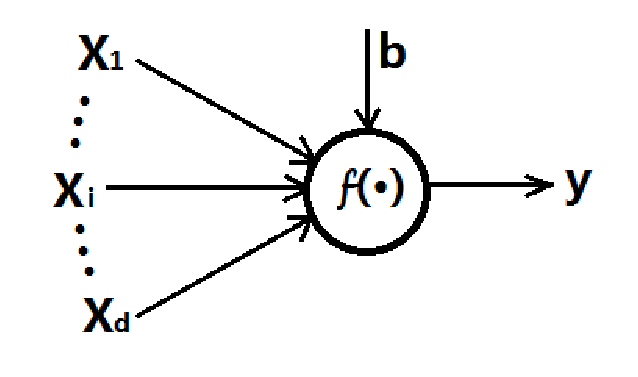
\includegraphics[width=0.33\textwidth]{DBN/NNnode.eps}
\caption{神经元}
\label{img:NNnode_cp5}
\end{figure}

与$d$个输入$x = [x_1, x_2\cdots, x_d]^T$直接相连的是数据的输入,例如,一章$28\times 28$像素的灰度图像作为网络输入,由于该图像可以展开成$28\times 28 = 784$的列向量,因此这个例子中的神经元就应该有784个输入,即$x = [x_1, x_2\cdots, x_{784}]^T$。$d$个权值$w = [w_1, w_2\cdots, w_d]^T$,刻画了$d$个输入$x = [x_1, x_2\cdots, x_d]^T$的重要性,$w$中的某个分量$w_i$越大,说明对应的分量$x_i$对最后决策结果的影响越大。从生物学的角度上看,$x$相当于给予生物各种刺激,$w$相当于该生物对各种刺激的敏感度。
例如,我们利用神经元设计一个医学诊断系统来判定一个人是否需要住院观察,对于该神经元,假设输入为$x = [\text{心脏疼痛},\text{头疼},\text{腰疼}]$,如果有某个症状,则对应位置1,否则置0。显然,若一个人心脏疼痛,我们更倾向于让他住院观察,因此我们为心脏疼痛对应的权值设定一个较大的权值$w_1 = 0.9$,头疼次之,我们设定为$w_2 = 0.5$,当一个人腰疼时,不太可能需要住院治疗,我们为其设定一个较小的偏置$w_3 = 0.1$。因此,这个神经元的权值为
\begin{equation}
w = [0.9, 0.5, 0.1]^T
\end{equation}

假设现在有一位患者来到医院,他既有头疼又有心脏疼痛的症状,那么这位患者可以表示为向量
\begin{equation}
x = [1, 0, 1]^T
\end{equation}
此时,病情积累的严重性为
\begin{equation}
w^Tx = 0.1+0.9 = 1
\end{equation}
那么这位患者是否需要住院呢?为此,我们利用前面提及到的偏置$b$来刻画这件事。假设$b = 0.7$,如果$w^Tx>b$,则说明这位患者患有严重的疾病,需要住院观察,网络输出$y=1$,否则这位患者不需要住院,网络输出$y=0$。如果我们定义为神经元的净激活为
\begin{equation}
net = w^Tx + b
\end{equation}
净激活可以理解为排除偏置干扰后神经元接收到的刺激总和。那么上述判别过程相当于用一个阶跃函数对净激活作一个非线性映射,即
\begin{equation}
y = f(net) = \left\{
\begin{array}{cc}
1 & \text{若}w^Tx - b> 0 \\
0 & \text{其他}
\end{array}
\right.
\end{equation}

其中,由于$b$是一个常数,因此$w^Tx +b$与$w^Tx - b$并没有区别。但实际上,$b = 0.7$时的神经元做出的决策,其结果只由心脏疼痛这个因素决定,因为如果一个患者没有心脏疼痛,那么最大的净激活是在他即患有头疼又患有腰疼的情况下取得,此时$net=0.6$。而$0.6<0.7$,并不会让他住院。因此,上面的神经元,转换成等价的逻辑命题便是:如果一个人的症状中含有心脏疼痛,则需要住院,否则不需要住院。如果我们把偏置调低,另$b=0.55$,则此时等价的逻辑命题为:如果一个人的症状中含有心脏疼痛,或者症状中既含有头痛有含有腰疼,则需要住院,否则不需要住院。综合以上讨论,偏置起到的是阈值的作用,但是这个阈值取多少就是设计者的意愿了,不同的阈值一般情况下会等价于不同的逻辑命题,这取决于系统的期望输出是什么。

神经元总能转换成一个对应的逻辑表达,需要提出的一个因果关系是,我们并不是从逻辑表达中推出神经元的参数,而是从神经元的参数中可以得到一个逻辑表达。神经元的优点在于,通过一个神经元,便可以实现一个简单的决策,如果拥有更多的神经元,将他们组合起来形成一个神经网络,便可以实现更为复杂的决策行为。这个决策的因果关系是由参数决定的,后面我们将会看到,参数是通过统计学习学到的,因此在神经网络中,我们不需要对事物的因果关系进行分析,只需要使用大量的数据让网络学习其中的因果关系,这些因果关系对于我们而言是透明的。


\BiSubsection{逻辑表达}
x在本小节,我们将再一次讨论网络的逻辑表达能力,如图\ref{img:NNnodeXY.png} 所示的一个接收两维输入的神经元,其偏置$w = [-2, -2]^T$,偏置$b=3$

\begin{figure}[!htbp]
\centering
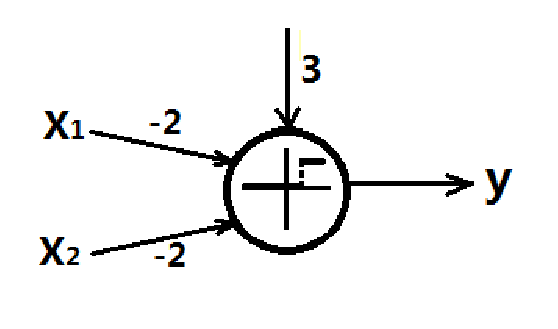
\includegraphics[width=0.33\textwidth]{DBN/NNnodeXY.eps}
\caption{与非门的神经元表达}
\label{img:NNnodeXY.png}
\end{figure}

如果我们的输入至少有一个为假,即$x = [0,0]^T$或$x = [1,0]^T$或$x = [0,1]^T$,则网络的输出为真,即$y=1$,若两个输入都为真,即$x = [1,1]^T$,则网络的输出为假,即$y=0$。事实上,图\ref{img:NNnodeXY.png}等价于逻辑电路中的与非门,即
\begin{equation}
y = \overline{ x_1\cdot x_2}
\end{equation}
由于与非门是通用们,可以利用多个与非门构建出三大逻辑门:与门、或门、非门。因此,利用图\ref{img:NNnodeXY.png}中的神经元可以表达任意一个逻辑函数。例如,在半加器中,其逻辑函数为
\begin{equation}
y_1 = x_1 \oplus x_2
\end{equation}
\begin{equation}
y_2 = x_1 \cdot x_2
\end{equation}
利用与非门搭建的电路图如图\ref{img:numberHalfAdd}所示,而将其转换成对应的神经网络如图\ref{img:NNhalfAdd}所示\footnote{图中,为了美观,我们并没有将偏置画出来}。

\begin{figure}[htbp]
\centering
\subfigure{\label{img:numberHalfAdd}}\addtocounter{subfigure}{-2}
\subfigure{\subfigure[由与非门搭建的半加器]
			{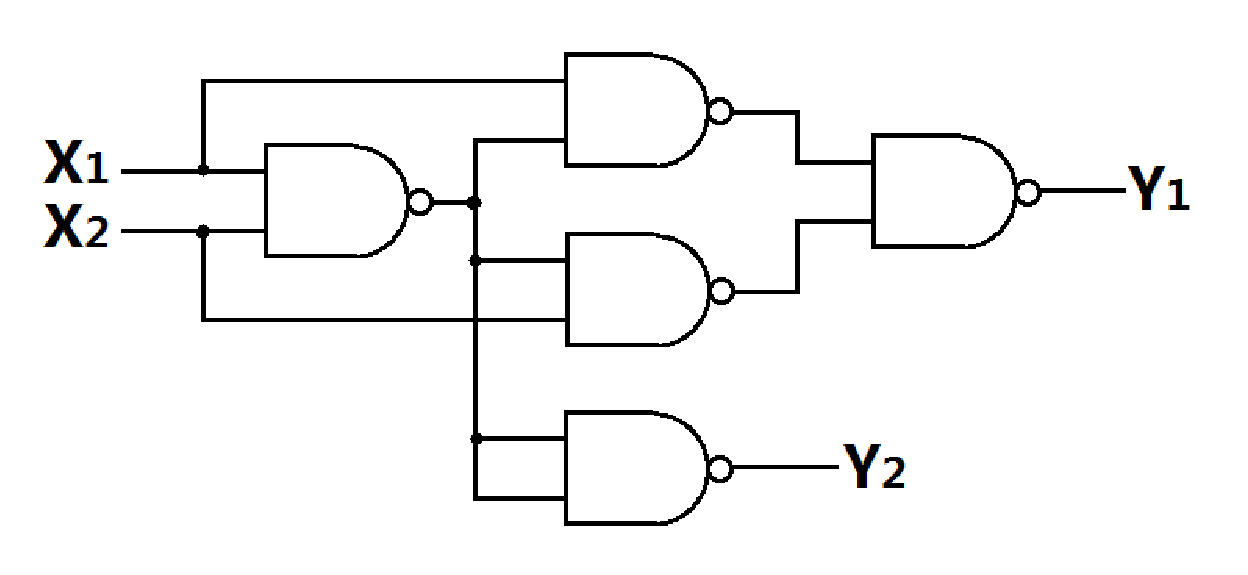
\includegraphics[width=0.5\textwidth]{DBN/numberCirc.eps}}}
\subfigure{\label{img:NNhalfAdd}}\addtocounter{subfigure}{-2}
\subfigure{\subfigure[由神经元搭建的半加器]
			{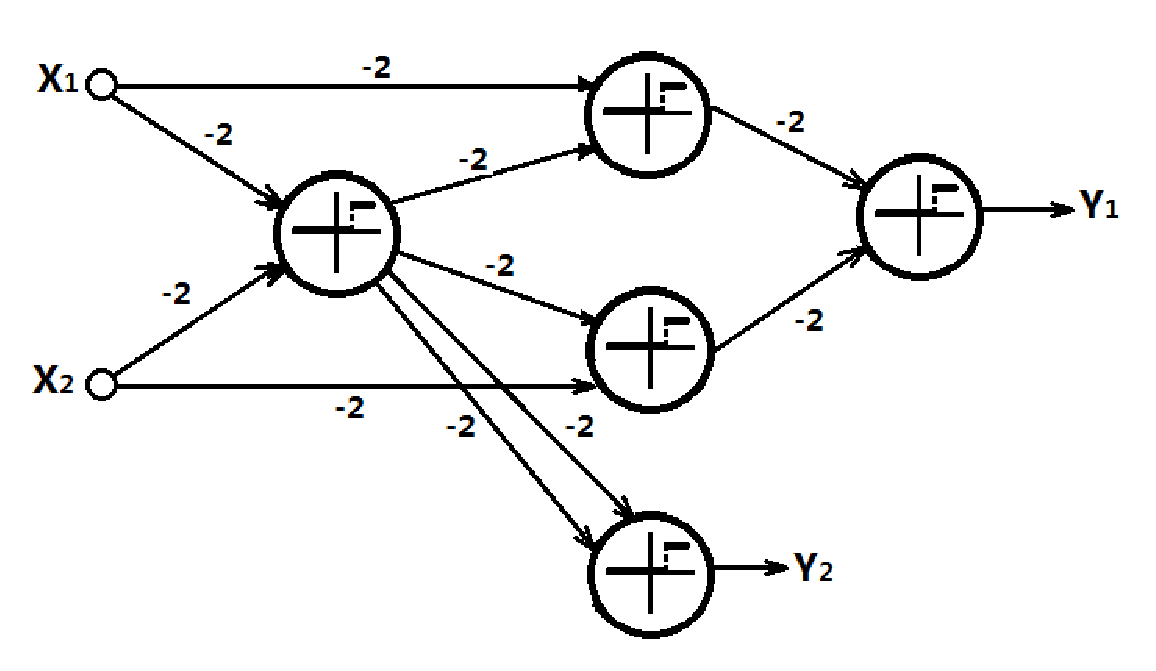
\includegraphics[width=0.4\textwidth]{DBN/NNCirc.eps}}}
\caption{半加器的两种不同描述}
\label{img:halfAdd}
\vspace{-1em}
\end{figure}

我们之所以花费篇幅去介绍神经元的表达能力,是为了说明神经网络确实能实现一些逻辑决策,但并不意味着网络的权值需要我们手工设定的。这里的权值之所以要手工设定,是因为我们精心筛选出来用以阐述神经网络的表达能力,但实际应用中,权值是通过误差传播自动学习的,学习到的权值,其对应的逻辑命题对于人类而言是难以理解的,但这并不重要,因为我们需要的是仅仅决策结果,而不是这个决策是如何产生的因果关系。

\BiSection{神经网络的前馈}
x一般而言,神经网络是一个多层结构组织,网络的每一层都由多个神经元阻生,上一层的神经元由下一层的神经元激活。同一层的神经元之间没有连接,因此同一层节点的激活是独立的。神经网络接收到一个数据后,逐层地激活各层的神经元,下一层的输出作为上一层的输入,最后得到一个输出结果。这个过程称为神经网络的前馈或前向传播。

\begin{figure}[!htbp]
\centering
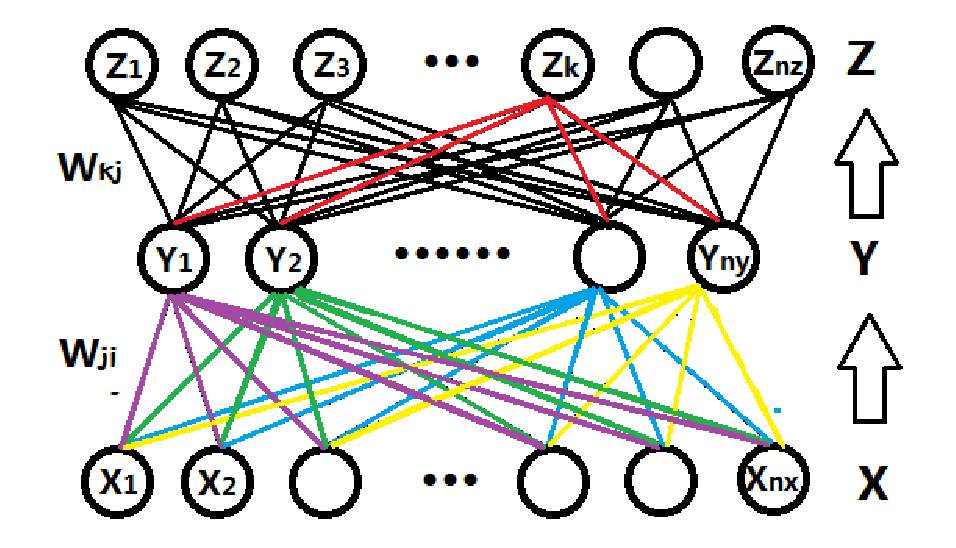
\includegraphics[width=0.55\textwidth]{DBN/3NNfp.eps}
\caption{神经网络的前馈}
\label{img:3NNfp}
\end{figure}

如图\ref{img:3NNfp}所示是一个三层神经网络,由于神经激活是自底向上传播的,如果各层的激活函数都相同,为$f(~\cdot~)$,则网络的第k个节点的输出为
\begin{equation}
z_k = f\bigg[\sum\limits_{j=1}^{n_y} w_{kj} 
f(\sum\limits_{i=1}^{n_x} w_{ji}) + b_j)
+ b_k\bigg]
\label{equ:DBN_NNoutput}
\end{equation}
式中,$w_{kj} $为$y$层的第$j$个节点到$z$层的第$k$个节点之间的连接权值,$w_{ji} $为$x$层的第$i$个节点到$y$层的第$j$个节点之间的连接权值,$b_j$为$y$层第$j$个节点的偏置,$b_k$为$z$层第$k$的节点的偏置。

神经网络的这种自底向上的激活,有时也被解释为特征提取或重新编码。当接收到一个数据时,神经网络将这个数据逐层地进行特征抽取,过滤掉一些冗余信息,将剩余的重新编码,最后利用一个分类器将抽取到的最抽象(即最顶层)特征进行分类,从而完成整个识别过程。

\BiSubsection{神经激活}
x到目前为止,我们只介绍了一种激活函数,即阶跃函数,但实际中我们并不会使用阶跃函数作为激活函数。首先,阶跃函数是不连续的,其次,阶跃函数是不可导的\footnote{事实上阶跃函数是可导的,其导函数为脉冲函数,这是一个广义函数,我们不深入讨论}。激活函数不可导,将导致网络无法利用反向传播进行训练,关于这点我们将在反向传播章节讨论。作为激活函数,它应该满足以下几个条件
\begin{enumerate}
\item 它必须是非线性的。由式\eqref{equ:DBN_NNoutput}可以看出,若激活函数是线性的,则多层神经网络实际上只相当于两层网络,因为多个矩阵相乘的结果为一个矩阵。网络一旦失去多层结构,则表达能力迅速下降。
\item 它应该具有饱和特性,即至少存在一个上界或下界。饱和特性的存在,使得神经元的输出不至于过高或过低,整个网络的编码维持在一定的范围内。但最近的研究表明,一些近似饱和的激活函数也能工作得很好,如此看来,饱和似乎并不是必要的,但近似饱和还是需要的。
\item 它应该连续且可导。由于反向传播中需要求取激活函数相对于净激活的偏导数,如果激活函数是不可导的,那么反向传播算法将无法执行。
\end{enumerate}
实际工程中,我们常用的激活函数是sigmoid函数\footnote{也被称为logistic函数}或双曲正切函数。其中,sigmoid函数我们定义为
\begin{equation}
f(net) = \frac{1}{1+ e^{-net}}
\end{equation}
其对应的图像如图\ref{img:sigmoid}所示
\begin{figure}[!htbp]
\centering
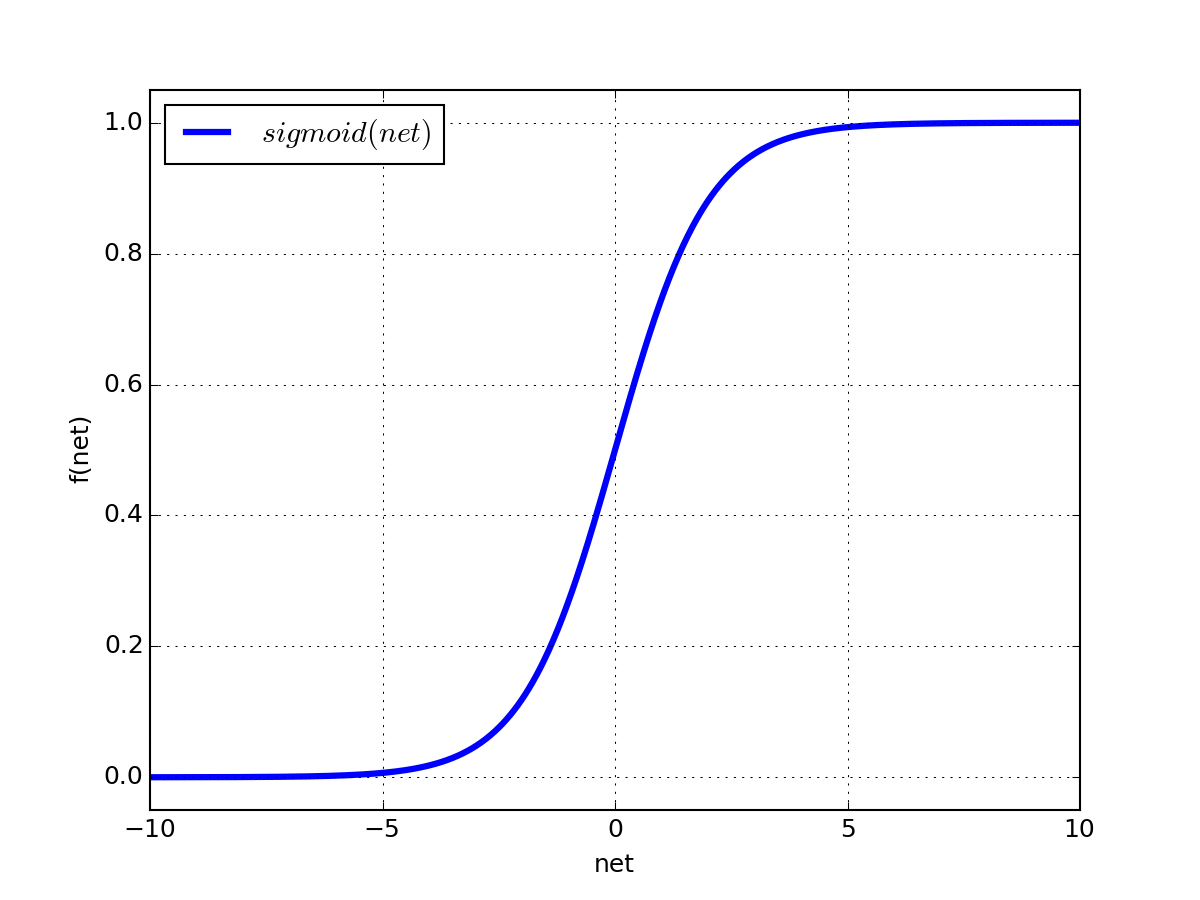
\includegraphics[width=0.5\textwidth]{DBN/sigmoid.eps}
\caption{sigmoid激活}
\label{img:sigmoid}
\end{figure}

可以看到,sigmoid函数是一个值域为$(0,1)$的连续可导函数,其导函数有一个重要特性,即
\begin{equation}
\begin{split}
f'(net) &= \frac{e^{-net}}{(1 + e^{-net})^2} = \frac{1}{1+ e^{-net}} -  \frac{1}{(1+ e^{-net})^2}\\
&=f(net)\Big[1 - f(net)\Big]
\end{split}
\label{equ:logisticDiff}
\end{equation}

这个特性之所以重要,是应为利用式\eqref{equ:logisticDiff}可以直接通过网络的输出直接计算激活函数相对于净激活的偏导数而不必引入额外的计算。我们看到,sigmoid函数的输出范围为$(0,1)$,有时候,我们希望网络的输出为$(-1,1)$,此时可以使用双曲正切函数,即
\begin{equation}
f(net) = \tanh(net) = \frac{e^{net} - e^{-net}}{e^{net} + e^{-net}}
\end{equation}
其对应的图像如图\ref{img:tanh}所示
\begin{figure}[!htbp]
\centering
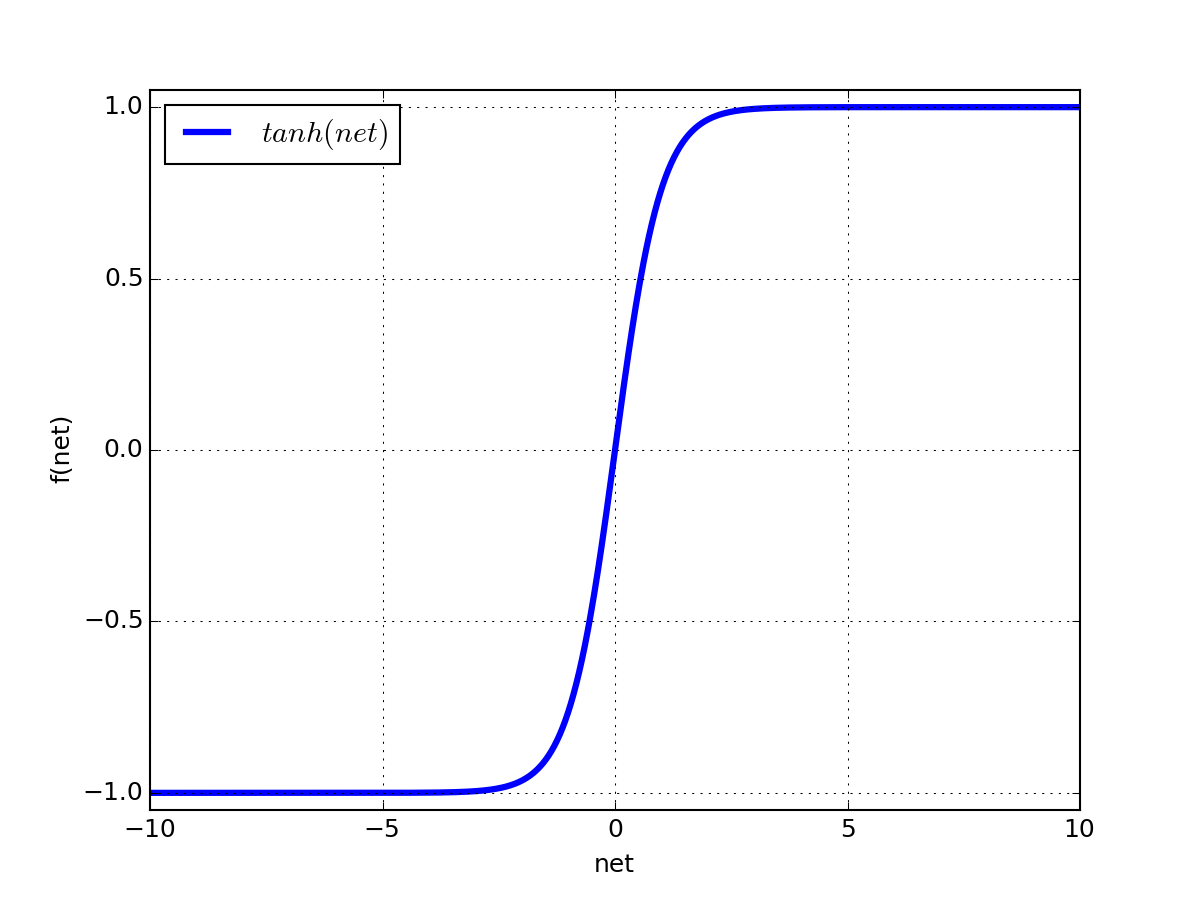
\includegraphics[width=0.5\textwidth]{DBN/tanh.eps}
\caption{tanh激活}
\label{img:tanh}
\end{figure}

近年来,在神经网络的研究上又提出了一些新的激活函数,其中最重要的莫过ReLU激活函数,其定义为\citeup{glorot2011deep}
\begin{equation}
f(net) = \left\{
\begin{array}{cc}
net & \text{若}net > 0\\
0 & \text{其他}
\end{array}
\right.
\label{equ:ReLU}
\end{equation}
式\eqref{equ:ReLU}也可以简写为
\begin{equation}
f(net) = \max (0, net)
\end{equation}
其对应的图像如图\ref{img:ReLU}所示
\begin{figure}[!htbp]
\centering
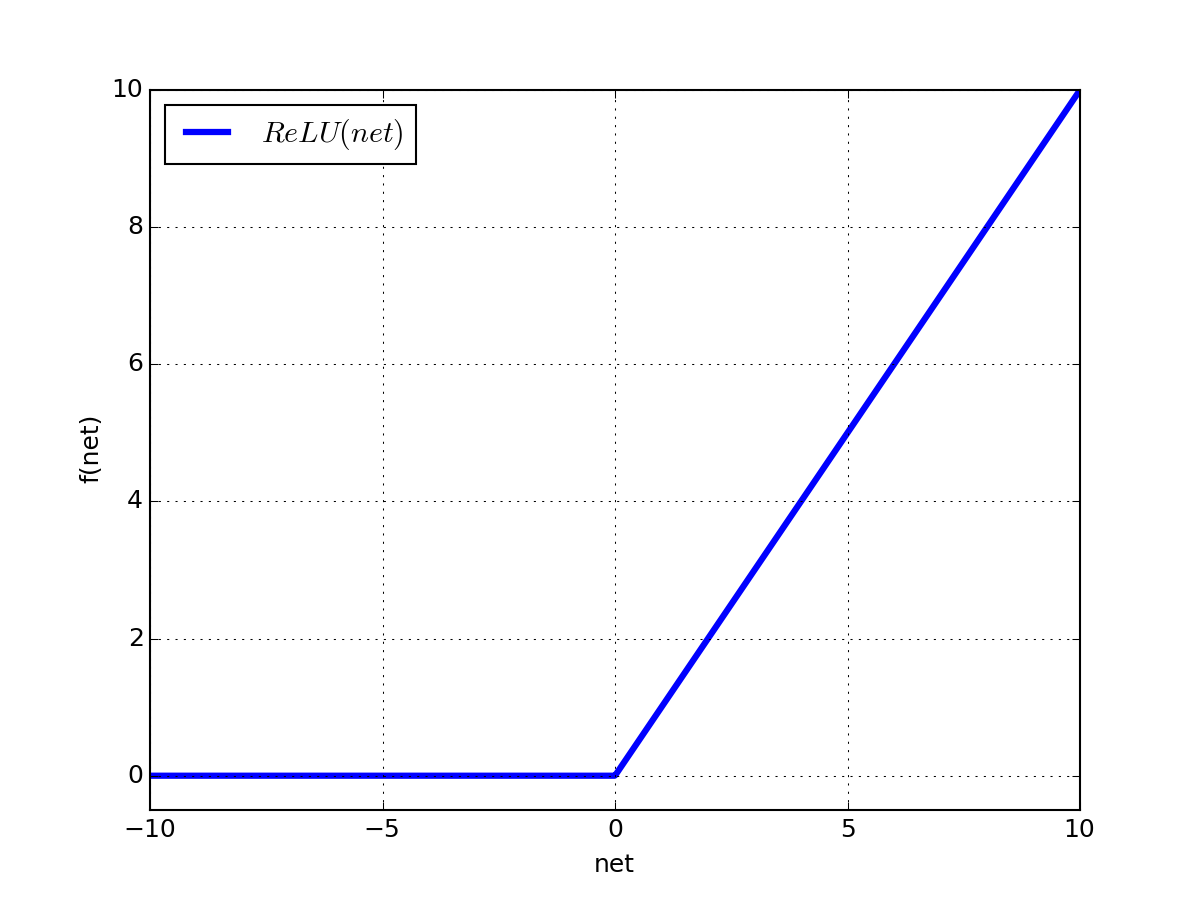
\includegraphics[width=0.48\textwidth]{DBN/ReLU.eps}
\caption{ReLU激活}
\label{img:ReLU}
\end{figure}

这种激活函数相比于sigmoid函数有较大的改进,关于其优点我们将留到反向传播的章节讨论。但ReLU有一个缺点:在$net<0$时导数为0,从而导致反向传播无法更新参数。因此,在ReLU的基础上又产生了一些变体,例如,softplus中,激活函数定义为\citeup{glorot2011deep}
\begin{equation}
f(net) = \log(1+e^{net})
\end{equation}
其对应的图像如图\ref{img:softplus}所示
\begin{figure}[!htbp]
\centering
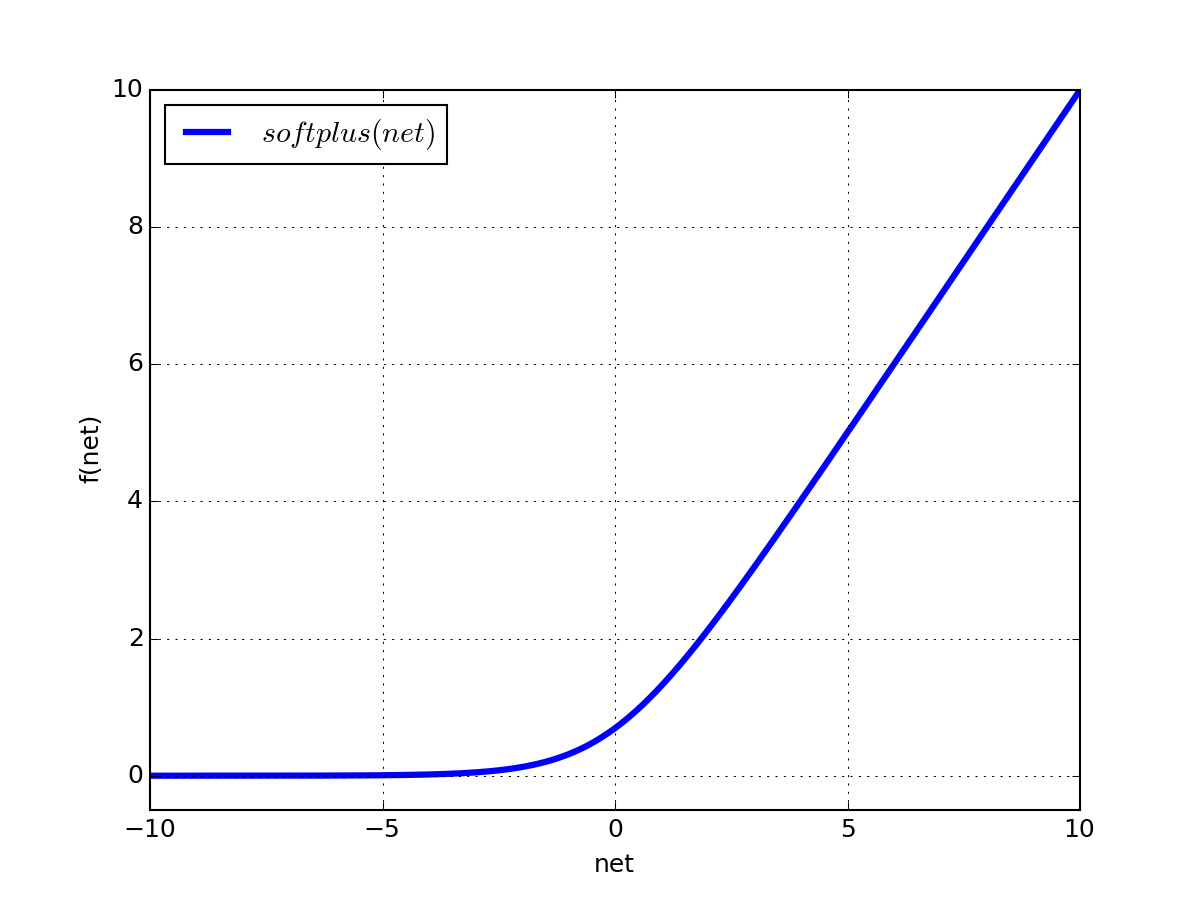
\includegraphics[width=0.48\textwidth]{DBN/softplus.eps}
\caption{softplus激活}
\label{img:softplus}
\end{figure}

从图中不难看出,softplus是ReLU的圆滑版,关于softplus,一个有意思的结论是,其激活函数的导数为logistics函数,即
\begin{equation}
f'(net) = \frac{e^{net}}{1 + e^{net}} = \frac{1}{1 + e^{-net}}
\end{equation}
然而这个结论并没有什么用处,因为它并不能减轻程序的计算量。

ReLU的另一种变体是由He Kaiming等人提出的PReLU,其激活函数定义为\citeup{MS2015}
\begin{equation}
f(net) = \left\{
\begin{array}{cc}
net & \text{若} net >0\\
\alpha net & \text{若} net \leq 0
\end{array}
\right.
\end{equation}
式中,$\alpha$为一个较小的参数,例如当$\alpha = 0.1$时,其图像如图\ref{img:PReLU}所示
\begin{figure}[!htbp]
\centering
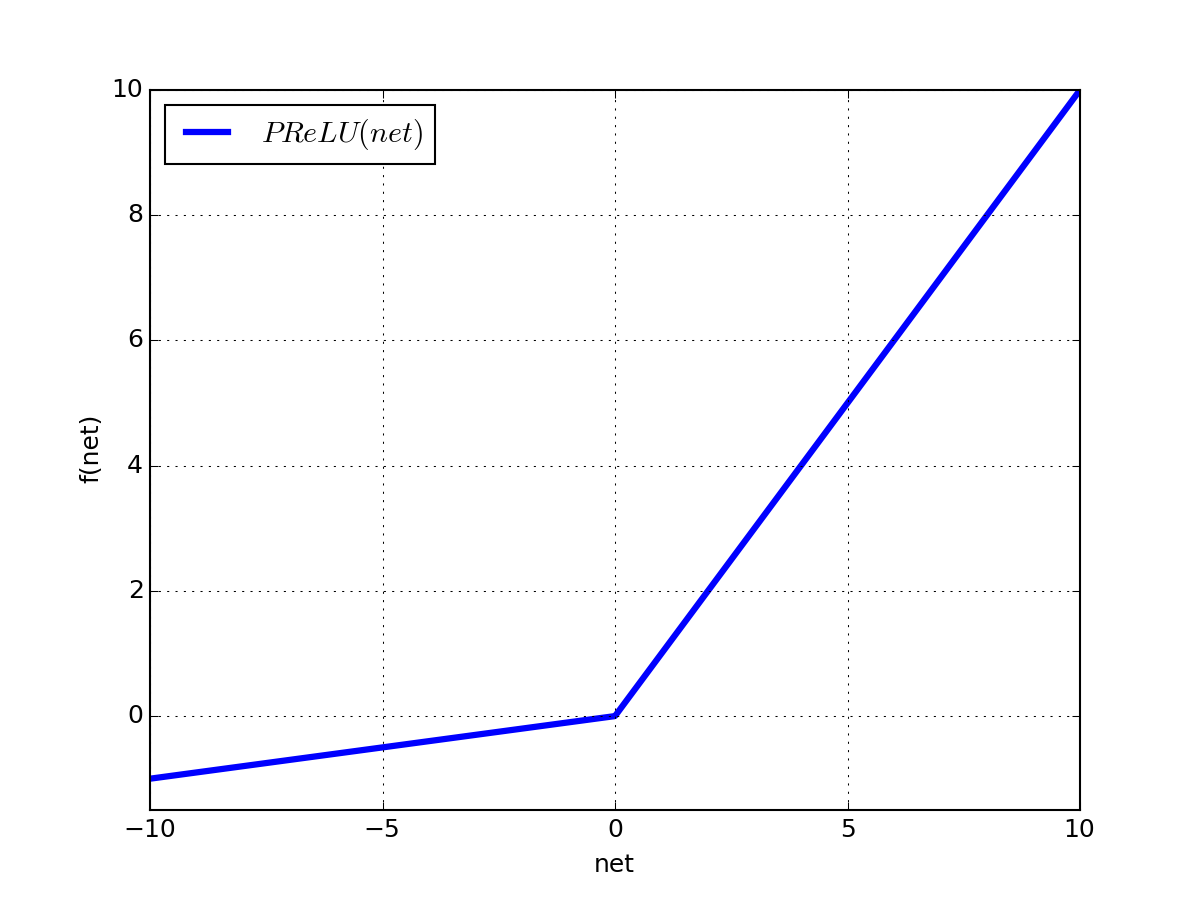
\includegraphics[width=0.5\textwidth]{DBN/PReLU.eps}
\caption{PReLU激活}
\label{img:PReLU}
\end{figure}

显然,PReLU在负半平面不再会出现导数为0的情况。尽管参数$\alpha$需要学习得到,但这种方法在ImageNet 2012数据集上获得了非常好的识别效果,首次在图像识别任务上超越了人的识别效果,错误率仅为4.94\%。在该文中,作者提到了一个有意思的现象:在较低层的网络中,学习到的参数$\alpha$较大,而在高层的网络中,参数$\alpha$较小。作者的猜测是较低曾网络需要尽可能多地保留数据的信息,因此激活函数更倾向于类线性,而高层网络更倾向于抽象数据的结构,从而做出决策,因此高层的激活函数更倾向于非线性。

在同一个任务中,激活函数的不同选取会有不同的实验现象,目前并没有证明哪种激活函数更好。习惯上,在全连接神经网络中,我们更喜欢sigmoid派的激活函数,而在卷积网络中,我们更喜欢ReLU派的激活函数,尽管这些都不是强制的。


\BiSection{分类器}
x神经网络的逐层激活,其本质在于将一种编码转化成另一种编码。编码之间的转换,可以过滤掉一些原始编码中无用的噪声或信息,这个过程一般都伴随着熵的减小(但并不绝对)。然而,一个神经网络在最顶层的激活,其编码是人类所无法理解的,因此,在最顶层节点之上还需要一个分类器对神经网络提取到的特征或者说编码进行分类。分类器其作用,一方面在于将编码转换为人类所能理解的编码,这在有监督的分类任务以及无监督的聚类任务中是必要的,因为我们最后希望网络能给我们一个输出标签。但对于降维任务而言有时候并不是必要的,因为降维并不需要输出标签。另一方面,分类器都带有一个准则函数,这个准则函数定义了熵,即定义了什么是混乱,什么是有序。从控制论的角度上看,控制工程中,误差是系统校正的核心,没有误差便没有反馈,没有反馈,则系统难以控制。机器学习也是同样的道理,没有误差,则无法对参数进行校正,机器便无法从样本中学习。误差的来源,源自于准则的定义,即预先预定什么是对的,什么是错的,对于错之间就会存在一个误差,如果机器产生了一个误差,利用这个误差便可以对参数进行校正。神经网络冲,常用的分类器有三种:平方误差、softmax、支撑向量机,尽管支撑向量机是一种重要的分类器,但是鉴于篇幅有限,我们并不打算在本文中介绍支撑向量机,关于其原理读者可参考文献xxxx。

\BiSubsection{平方误差分类器}
x严格来说,平方误差并不能算作一个分类器,它充其量只能算作一个准则,这个准侧除了在神经网络中有应用之外,在很多领域也有广泛的应用。平方误差,或者说二范数,其准则函数定义为
\begin{equation}
L = \sum\limits_{i=1}^d (x_i -t_i)^2
\label{equ:L2error}
\end{equation}
式中,$x_i$为网络的输出,这个输出由输入数据与网络参数共同决定,$t_i$代表标签值,也成为教师信号,由数据的标签值决定,$d$则是$x$的维数。假设一个神经网络的最顶层有4个节点,网络的输出为$[~-0.1~~0.1~~0.8~~0.1~]$,而我们的期望输出是$[~0~~0~~1~~0~]$(再一次强调,这个期望输出由标签值决定),那么实际输出与期望输出之间就会存在一个误差向量$[~-0.1~~0.1~~0.2~~0.1~]$,将其转化成平方误差后为$[~0.01~~0.01~~0.04~~0.01~]$,利用式\eqref{equ:L2error}可以很容易算的此时$L=0.07$。事实上,$L=0.07$对我们而言没有太大用处,它最多只能刻画总的误差量有多大,真正对我们有用的是平方误差向量,利用这个向量,可以将误差反向传播回神经网络的底层,从而自顶向下就网络参数进行校正,关于这个过程更多的细节,我们将会留到反向传播章节介绍。

\BiSubsection{softmax分类器}
x实际中,为了方便分类,我们往往希望网络的输出是“k中取1”的形式,例如,假设我们有四个类别,如果使用二进制编码的话,我们只需两个节点即可,即00代表第一类,01代表第二类,以此类推。如果我们使用所谓的“k中取1”形式,我们便需要四个节点,即0001代表第一类,0010代表第二类,0100代表第三类,1000代表第四类。为了实现“k中取1”的形式,我们需要引入softmax分类器,softmax分类器可以认为是logistics回归的推广,在使用logistics回归进行分类时,只能实现两类分类,而softmax分类器可以实现多类分类功能。

在softmax分类器中,假设容量为$n$的训练集为$S = \big\{(x^{(1)}, y^{(1)}), \cdots, (x^{(n)}, y^{(n)})\big\}$,由于标签$y$的取值可以有$c$种,因此$y^{(i)} \in \{1, 2,  \cdots, c\}$。我们引入记号$(\phi_1, \phi_2, \cdots, \phi_c)$来表示各个类别的输出概率,由于$\sum\phi_i = 1$,因此记号存在冗余,只需要$c - 1$个记号$(\phi_1, \phi_2, \cdots, \phi_{c-1})$即可,对于$\phi_i$,有
\begin{equation}
\phi_i = P(y = 1; \phi)
\end{equation}
以及
\begin{equation}
\phi_c = P(y = c; \phi) = 1 - \sum\limits_{i=1}^{c-1}\phi_i
\end{equation}
注意,正如我们之前提到的,$\phi$中参数存在冗余,所以$\phi_c$并不是参数,而是一个为了方便后面讨论所引入的一个记号。

由于softmax的概率分布也属于指数分布族,而在指数分布族中,对于概率分布而言,都可以写成如下形式
\begin{equation}\label{equ:expFamily}
P(y; \eta) = b(y) \exp \bigg[\eta^T T(y) - a(\eta)\bigg]
\end{equation}

在softmax中,我们记$T(y) \in R^{c-1}$为

\begin{equation}
T(1) = \left[               %左括号
\begin{array}{cccc}  
1\\  
0\\
\vdots\\
0
\end{array}
\right]~~~~%%%%%%%%%%%%%%%%%%%%
T(2) = \left[   
\begin{array}{cccc}  
0\\  
1\\
\vdots\\
0
\end{array}
\right]~~~~~~%%%%%%%%%%%%%%%%%%%
\cdots~~~~~~
T(c-1) = \left[   
\begin{array}{cccc}  
0\\  
0\\
\vdots\\
1
\end{array}
\right]~~~~%%%%%%%%%%%%%%%%
T(c) = \left[   
\begin{array}{cccc}  
0\\  
0\\
\vdots\\
0
\end{array}
\right]~~~~%%%%%%%%%%%%%%%%%%%%%% 
\end{equation}
记$\Big[T(y)\Big]_i$为$T(y)$的第$i$个元素,记$1 \{\cdot\}$为示性函数,即
\begin{equation}
1 \{A\} = \left\{
\begin{array}{cc}
1 & \text{,若命题$A$为真} \\
0 & \text{,若命题$A$为假}
\end{array}
\right.
\end{equation}
因为$\Big[T(y)\Big]_i = 1\{y = i\}$,因此
\begin{equation}
\begin{split}
\mathbb{E}\bigg[\big[T(y)\big]_i\bigg] &= \big[T(y)\big]_i \cdot P(y = i) \\
&= P(y=i)  \\
&= \phi_i
\end{split}
\end{equation}

而
\begin{equation}
\begin{split}
P(y; \phi) &= \phi_1^{1\{y=1\}} \phi_2^{1\{y=2\}}\cdots\phi_c^{1\{y=c\}} \\
&=\phi_1^{1\{y=1\}} \phi_2^{1\{y=2\}}\cdots\phi_c^{1 - \sum\limits_{i=1}^{c - 1}1\{y = i\}} \\
&=\phi_1^{\big[T(y)\big]_1}\phi_2^{\big[T(y)\big]_2}\cdots\phi_c^{1 - \sum\limits_{i=1}^{c-1}\big[T(y)\big]_i}\\
&=\exp\bigg\{\ln\Big[\phi_1^{\big[T(y)\big]_1}\phi_2^{\big[T(y)\big]_2}\cdots\phi_c^{1 - \sum\limits_{i=1}^{c-1}\big[T(y)\big]_i}\Big]\bigg\} \\
&=\exp\bigg\{ \Big[T(y)\Big]_1\ln\phi_1 + \Big[T(y)\Big]_2\ln\phi_2+\cdots + \bigg[1-\sum\limits_{i=1}^{c-1}\Big[T(y)\Big]_i \bigg]\ln\phi_c \bigg\}\\
&=\exp\bigg\{\Big[T(y)\Big]_1\ln\frac{\phi_1}{\phi_c} + \Big[T(y)\Big]_2\ln\frac{\phi_2}{\phi_c} + \cdots  +  \ln \phi_c \bigg\}
\end{split}
\end{equation}
对比式\eqref{equ:expFamily},得
\begin{equation}
b(y) = 1
\end{equation}
\begin{equation}
\eta = \Big[~~\ln\frac{\phi_1}{\phi_c}~~~~\ln\frac{\phi_2}{\phi_c}~~~~\cdots~~~~\ln\frac{\phi_{c-1}}{\phi_c}~~\Big]^T
\end{equation}
\begin{equation}
a(\eta) = -\ln\phi_c
\end{equation}
定义
\begin{equation}
\eta_i = \ln\frac{\phi_i}{\phi_c}~~~~~~~~\eta_c = \ln \frac{\phi_c}{\phi_c}=0
\end{equation}
由于
\begin{equation}
e^{\eta_i} = \frac{\phi_i}{\phi_c}
\end{equation}
则
\begin{equation}
\phi_c\cdot e^{\eta_i} = \phi_i
\end{equation}
且
\begin{equation}
\phi_c\sum\limits_{i=1}^c e^{\eta_i}= \sum\limits_{i=1}^c \phi_c e^{\eta_i}
=\sum\limits_{i=1}^k\phi_i
=1
\end{equation}
从而
\begin{equation}
\phi_i = \phi_c e^{\eta_i} = \frac{\exp(\eta_i)}{\sum_{i=1}^c \exp(\eta_i)}
\end{equation}
即
\begin{equation}
P(y=i;\phi) = \phi_i =\frac{\exp(\eta_i)}{\sum_{i=1}^c \exp(\eta_i)}
\end{equation}
以及
\begin{equation}
P(y=i|x;\theta) = \frac{\exp(\theta_i^Tx)}{\sum_{j=1}^c\exp(\theta_j^T x)}
\end{equation}

本质上,softmax分类器都可以看做是一种两层神经网络,与常规的神经网络中使用sigmoid函数作为激活函数不同,在softmax分类器中,激活函数$f(net_k) \propto e^{net_k}$,对应的激活概率定义为\citeup{Duda}
\begin{equation}\label{temp3}
z_k = \frac{e^{net_k}}{\sum_{i=1}^c e^{net_i}}
\end{equation}
式中,$z_k$代表第$k$个节点激活的概率,$net_k$代表第$k$的节点的净激活,取值为输入特征$x$的线性函数,即$net_k = \theta_k  x^T$,$c$为类别的总数。在式\eqref{temp3}中分母的作用下,我们对每个类别的输出都进行了归一化,所以总的激活概率为1。在识别中,计算各个类别的激活概率后,只需选取最大激活概率所对应的类别作为输出类别即可。

\BiSection{神经网络的反馈}
x神经网络的反馈是基于准则函数的反馈,准则函数作为误差的度量,刻画了网络的输出与训练集的标签两者之间的差异。整个反馈过程中,实质上就是准则函数最小化的过程,即对网络的参数进行更新,使得误差不断减小。假设一个以参数$\theta$为自变量的准则函数$f(\theta)$,反馈过程就相当于不断寻求$\theta$使得$f(\theta)$最小的过程。如果$f(\theta)$是凸的,即Hessian矩阵是正定的,那么我们称这个问题为凸优化问题,我们可以有很多策略解决凸优化问题,但实际中遇到的问题基本都是非凸问题,解决非凸问题,一个简单有效的方法是利用梯度下降。想象我们在一座山上,为了更快速的下山,我们可以每一步都朝着当前最陡峭的方向(即梯度方向)前进,梯度下降也是基于这个原理,每一次迭代,我们都在当前的$\theta$下计算$f(\theta)$的梯度$\Delta_\theta f(\theta)$,让$\theta$加上这个梯度分量,也就是让它朝着梯度下降的方向迭代。由于梯度下降的每一步都是基于当前的参数$\theta$,所以这是一个贪婪算法,并不能保证收敛到全局最优。如果$f(\theta)$是凸的,那么梯度下降在大部分情况下它会收敛到全局最优(但并不绝对),然而,实际任务由于其非凸性,我们基本上不可能收敛到全局最小值,我们得到的往往是局部极小值。另外,值得一提的是,收敛到全局最小值是没有意义的,因为这个全局最小值是基于训练集的最小值,一旦收敛到此处,意味着网络可以很好地刻画训练集,但并不意味它同样可以很好地泛化到测试集上,这个时候往往会伴随着较高的过拟合风险,我们不应一味地最求全局最小,而应在训练集与测试集两者之间进行一个权衡。梯度下降,因其简单有效的特点,称为优化问题中一个很常用的策略。
\BiSubsection{分类器参数校正}
x20世纪80年代以前,人们并没有找到一个较好的方法训练神经网络,这种状况一直维持到1986年,在这一年里由Rumelhart与Mecelland为首的科学家小组\footnote{事实上反向传播是由很多人在同一年代同时独立提出的} 提出了方向传播算法,首次在神经网络中利用梯度下降逐层地训练网络参数,每训练完一层后将当前层的误差传递回下一层,依次迭代,最后完成整个网络的训练。在这套方法中,核心点有两个:如何利用最顶层(即分类器)的误差来更新最顶层的参数以及如何在某一层网络更新完参数后将该层的误差传播回前一层,我们将会在本小节中讨论最顶层的参数校正,并在下一小节讨论误差传播。
\BiSubsubsection{平方误差分类器参数校正}
x由于在平方误差分类器中,准则函数定义为
\begin{equation}
J(\theta) = \frac{1}{2}\sum\limits_{i=1}^c(t_i - z_i)^2 = \frac{1}{2}||t-z||^2
\end{equation}
式中,$z_i$为训练集的标签值,而网络的输出$t_i$又是由前一层的静激活经过非线性映射后得到的,即
\begin{equation}
t_i = f(net_i)
\end{equation}
式中,$net_i$为输出层的前一层,即倒数第二层的净激活,而这个净激活又被定义为
\begin{equation}
net_i = wx + b
\end{equation}
式中,$w$为输出层与倒数第二层两者之间的权值,$b$为偏置,因此,我们不难通过链式求导得到误差相对于参数的梯度,即$J(\theta)$相对于$\theta$(这里的$\theta$即为$w$和$b$)的导数
\begin{equation}
\frac{\partial J(\theta)}{\partial w} = \frac{\partial J(\theta)}{\partial net} \frac{\partial net}{\partial w}\label{equ:5.0}
\end{equation}
以及
\begin{equation}
\frac{\partial J(\theta)}{\partial b} = \frac{\partial J(\theta)}{\partial net} \frac{\partial net}{\partial b}\label{equ:5.00}
\end{equation}
如果此时的激活函数是sigmoid函数,那么容易知道
\begin{equation}
\frac{\partial J(\theta)}{\partial net} = net(1-net)\label{equ:5.1}
\end{equation}
如果激活函数是ReLU函数,也容易得到
\begin{equation}
\frac{\partial J(\theta)}{\partial net} = \left\{
\begin{array}{cc}
1 & \text{若}net>0\\
0 &\text{若}net\leq 0\\
\end{array}
\right.\label{equ:5.2}
\end{equation}
而$\partial net/\partial \theta$只是一个线性函数,同样容易求得
\begin{equation}
\frac{\partial net}{\partial w} = x~~~~~~~~\frac{\partial net}{\partial b} = 1\label{equ:5.3}
\end{equation}
利用\eqref{equ:5.1}或\eqref{equ:5.2}\footnote{这取决于你的激活函数选取}以及\eqref{equ:5.3}便可以求取式\eqref{equ:5.0}以及\eqref{equ:5.00}中参数应该修改的幅度,即梯度。






\BiSubsubsection{softmax分类器参数校正}
在softmax的训练中,由于我们的期望输出为
\begin{equation}
h_\theta(x) =\mathbb{E}\Big[T(y)|x;\theta \Big]
%%%%%%%%%%%%%%%%%%%%%%%%%%%
=\mathbb{E}\left[
\begin{array}{cccc}
1\{y=1\}\\
1\{y=2\}\\
\vdots\\
1\{y=c-1\}
\end{array}
\right | x; \theta
\left.
\begin{array}{cccc}\\\\\\\\\end{array}
\right]
%%%%%%%%%%%%%%%%%%%%%%%%%%%
=\left[
\begin{array}{cccc}
\phi_1\\
\phi_2\\
\vdots\\
\phi_{c-1}
\end{array}
\right] 
%%%%%%%%%%%%%%%%%%%%%%%%%%%
=\left[
\begin{array}{cccc}
\frac{\exp(\theta_1^T x)}{\sum_{j=1}^c \exp(\theta_j^T x)}\\
\frac{\exp(\theta_2^T x)}{\sum_{j=1}^c \exp(\theta_j^T x)}\\
\vdots\\
\frac{\exp(\theta_{c-1}^T x)}{\sum_{j=1}^c \exp(\theta_j^T x)}
\end{array}
\right]
\end{equation}
对应的似然函数为
\begin{equation}
\mathcal{L}(\theta) = \prod\limits_{i=1}^n P(y^{(i)}|x^{(i)}; \theta)
\end{equation}
对应的对数似然函数为
\begin{equation}\label{equ:softmaxErr}
\begin{split}
\ell(\theta) &= \sum\limits_{i=1}^n\ln P(y^{(i)}|x^{(i)}; \theta)\\
&=\sum\limits_{i=1}^n\sum\limits_{j=1}^c \ln \bigg(\frac{\exp(\theta_j^Tx^{(i)})}{\sum_{t=1}^c\exp(\theta_t^T x^{(i)})} \bigg)^{1\{y^{(i)} = j\}}\\
&=\sum\limits_{i=1}^n\sum\limits_{j=1}^c 1\{y^{(i)} = j\} \ln \bigg(\frac{\exp(\theta_j^Tx^{(i)})}{\sum_{t=1}^c\exp(\theta_t^T x^{(i)})} \bigg)
\end{split}
\end{equation}
式\eqref{equ:softmaxErr}的相反数也被称为交叉熵,在训练过程中充当准则函数,我们对其求导,有
\begin{equation}
\begin{split}
\frac{\partial \ell (\theta)}{\partial\theta_j} 
&=\sum\limits_{i=1}^n\sum\limits_{j=1}^c 1\{y^{(i)} = j\}\bigg[x^{(i)} - \frac{\partial}{\partial\theta_j}\ln \sum\limits_{t=1}^c \exp\big(\theta_t^T x^{(i)}\big)\bigg]\\
&=\sum\limits_{i=1}^n\sum\limits_{j=1}^c 1\{y^{(i)} = j\} \bigg[ x^{(i)} - \frac{\exp(\theta_j^T x^{(i)})}{\sum_{t=1}^c\exp(\theta_t^T x^{(i)})} x^{(i)}\bigg]\\
&=\sum\limits_{i=1}^n\sum\limits_{j=1}^c 1\{y^{(i)} = j\} x^{(i)} \bigg[1 - P(y^{(i)} = j|x^{(i)}; \theta)\bigg]
\end{split}
\end{equation}
由于$1\{y^{(i)} = j\} \in \{0, 1\}$,所以写成向量形式为
\begin{equation}\label{equ:softmaxGrid}
\frac{\partial \ell (\theta)}{\partial\theta_j}  = \sum\limits_{i=1}^n x^{(i)} \Big[1\{y^{(i)} = i\} - P(y^{(i)}=j|x^{(i)}; \theta)\Big]
\end{equation}
通过使用式\eqref{equ:softmaxGrid}进行迭代,我们便可以使用梯度上升(下降)进行搜索,从而最大化似然(或最小化交叉熵)来训练softmax分类器。

\BiSubsection{误差传播}
x为了简单起见,我们使用一个三层神经网络对误差传播进行讨论,但通过这里的讨论,我们可以很容易将神经网络扩展到多层结构。
\begin{figure}[!htbp]
\centering
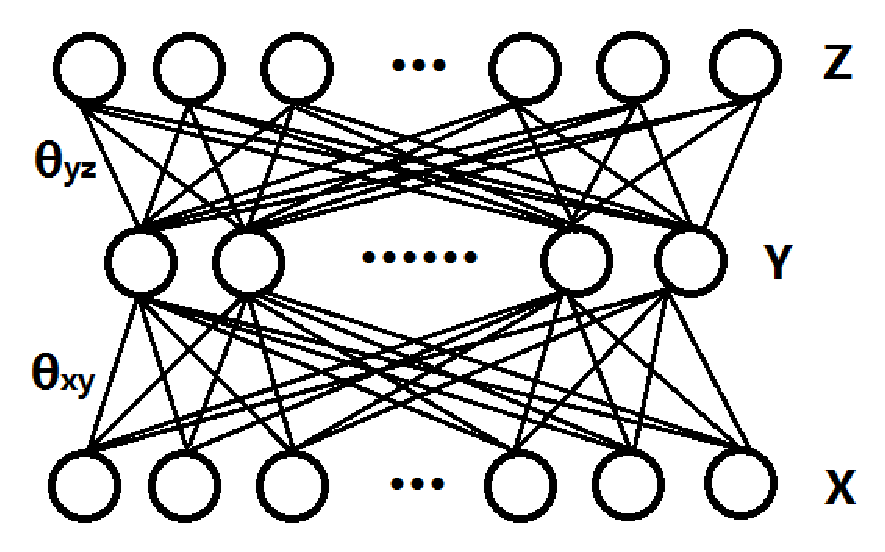
\includegraphics[width=0.4\textwidth]{3NN.eps}
\caption{三层神经网络的网路构型}
\label{img:3NN}
\end{figure}
如图中的三层神经网络,$y$层到$z$层为分类器,根据之前的讨论,我们可以利用式\eqref{equ:5.0}和式\eqref{equ:5.00} 求取$\partial J(\theta)/\partial \theta_{yz}$的值,如果我们要求取$\partial J(\theta)/\partial \theta_{xy}$的值,那么通过链式求导,我们有
\begin{equation}
\frac{\partial J(\theta)}{\partial\theta_{xy}} = \frac{\partial J(\theta)}{\partial y} \frac{\partial y}{\partial net_y} \frac{\partial net_y}{\partial \theta_{xy}}\label{equ:xxxxx}
\end{equation}
而我们又可以求得
\begin{equation}
\frac{\partial J(\theta)}{\partial y} =  \frac{\partial J(\theta)}{\partial net_z} \frac{\partial net_z}{\partial y}\label{equ:5.0.5}
\end{equation}
如果我们定义式\eqref{equ:5.0}以及式\eqref{equ:5.00}中的误差为
\begin{equation}
\delta_z = \frac{\partial J(\theta)}{\partial net_z}
\end{equation}
那么我们可以将式\eqref{equ:5.0.5}写为
\begin{equation}
\frac{\partial J(\theta)}{\partial y}  =  \delta_z \frac{\partial net_z}{\partial y} = \delta_z \theta_{yz}^T
\end{equation}
式中,$\partial J(\theta) /\partial y$就是分类器输出层(Z层)的误差传播回其上一层(Y层)的误差,如果我们定义Y层的误差为
\begin{equation}
\delta_y = \frac{\partial J(\theta)}{\partial y} \frac{\partial y}{\partial net_y}
\end{equation}
则我们可以利用后一层传播回来的误差$\delta_z$计算该层的误差
\begin{equation}
\delta_y = \delta_z \theta_{yz}^T  \cdot \frac{\partial y}{\partial net_y}
\end{equation}
从而我们可以利用该层的误差$\delta_y$计算该层参数$w_{xy}$的增量,即梯度
\begin{equation}
\frac{\partial J(\theta)}{\partial\theta_{xy}} =\delta_y \cdot  \frac{\partial net_y}{\partial \theta_{xy}}\label{equ:yyyyy}
\end{equation}
通过式\eqref{equ:yyyyy}对参数$\theta_{xy}$进行校正,校正完毕后,如果网络不止三层,而是四层,假设X层的下一层为P层,那么为了计算连接X层与P层参数$\theta_{px}$的梯度,利用链式求导,同样有
\begin{equation}
\frac{\partial J(\theta)}{\partial\theta_{px}} = \frac{\partial J(\theta)}{\partial x} \frac{\partial x}{\partial net_x} \frac{\partial net_x}{\partial \theta_{px}}\label{equ:zzz}
\end{equation}
与之前的做法类似,我们有
\begin{equation}
\begin{split}
\frac{\partial J(\theta)}{\partial x} & = \frac{\partial J(\theta)}{\partial y}  \frac{\partial y}{\partial net_y}\frac{\partial net_y}{\partial x}\\
&=\delta_y \cdot \theta_{xy}^T
\end{split}
\end{equation}
同样的道理,X层的误差$\delta_x$定义为
\begin{equation}
\delta_x =   \frac{\partial J(\theta)}{\partial x} \frac{\partial x}{\partial net_x} = \delta_y  \theta_{xy}^T \cdot \frac{\partial x}{\partial net_x}
\end{equation}
则参数$\theta_{px}$的梯度便可以利用$\delta_x$计算
\begin{equation}
\frac{\partial J(\theta)}{\partial\theta_{px}} = \delta_x \cdot \frac{\partial net_x}{\partial \theta_{px}}
\end{equation}
如果还有更多的层,其原理雷同,我们不再详细叙说。现在让我们抛开以上的数学内容从网络的结构上解释这个算法为什么叫做误差反向传播,首先我们观察各层的误差,即
\begin{equation}
[\delta_z~~\delta_y~~\delta_x ] = \bigg[~~
\frac{\partial J(\theta)}{\partial net_z}~~~~~~
\delta_z \theta_{yz}^T  \cdot \frac{\partial y}{\partial net_y}~~~~~~
\delta_y  \theta_{xy}^T \cdot \frac{\partial x}{\partial net_x}
~~\bigg]\label{equ:delta inject}
\end{equation}
式中,$\theta^T$起到的作用是将误差$\delta$反向注入的行为,这个行为如图\ref{img:3NNbp}所示
\begin{figure}[!htbp]
\centering
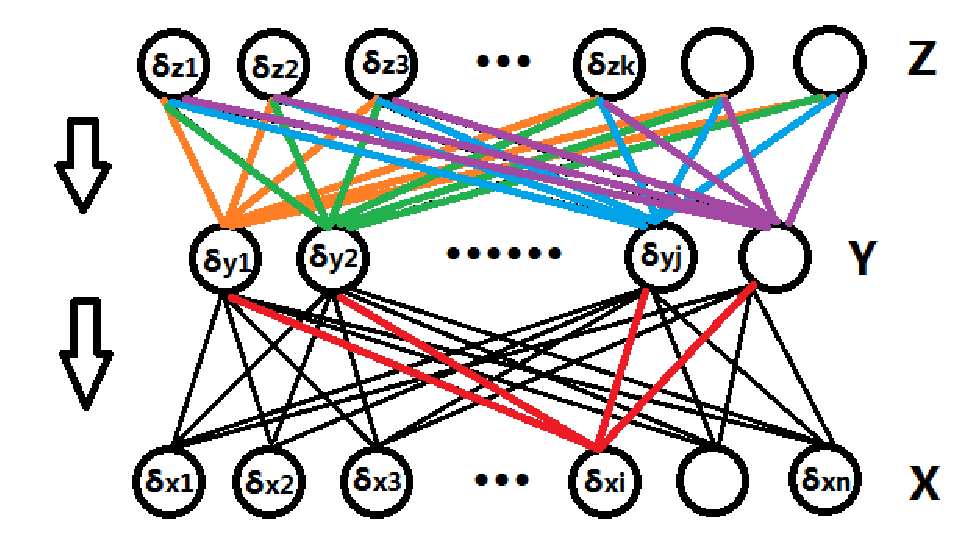
\includegraphics[width=0.55\textwidth]{DBN/3NNbp.eps}
\caption{误差反向注入}
\label{img:3NNbp}
\end{figure}

观察式\eqref{equ:delta inject},我们不难看出,除了最顶层外,剩余层的误差形式都是类似的,如果用一句话概括反向传播算法,便是:将$\ell$层的误差注入到$\ell - 1$层中,再乘上$\ell -1$层激活函数的导数,得到$\ell - 1$层的误差,利用这个得到的误差,对$\ell - 1$层的参数进行更新,更新完毕后,将$\ell - 1$层的误差重新注入到$\ell - 2$层,重复上述步骤直至误差传遍整个网络。但是这里有个例外,最顶层的误差定义与剩余层的不一样,之所以会这样是因为最顶层的误差并不是通过注入方式得到的,而是人为定义得到的,因为这个误差源自于准则函数。

我们可以看到,反向传播这种策略实际上与前向传播是类似的,反向传播也是一种贪婪算法,这将会导致一些问题。因为每一次误差传播都是更新参数后再将误差注入回前一层,这并不能保证计算得到的梯度就是真实的梯度,一旦网络的层数过深,将会导致前面层的真实导数与利用反向传播计算得到的导数相差过大。另外,如果使用sigmoid函数作为激活函数,它将很容易进入饱和状态,前面层的梯度接近于0,从而参数无法更新,这种现象我们称之为梯度消失。一种对抗梯度消失的方法是将sigmoid函数换成ReLU激活函数,关于ReLU为什么可以抵抗梯度消失的原理目前尚未研究出来,但是实验现象表明它确实能抑制梯度消失。

\BiSection{深度置信网络}
x深度置信网路(Deep Belief Networks,简写为DBN)本质就是一种传统的神经网络,但是它在传统神经网络的基础上加入一些变动。首先,这是一种深层的神经网络,而传统的神经网络一般只设计为三层结构。另外,深度置信网络是一个以受限玻尔兹曼机为基础,多个受限玻尔兹曼机垒出来的多层神经网络。图\ref{img:DBN}展示了一个深度为4的深度置信网络。
\begin{figure}[!htbp]
\centering
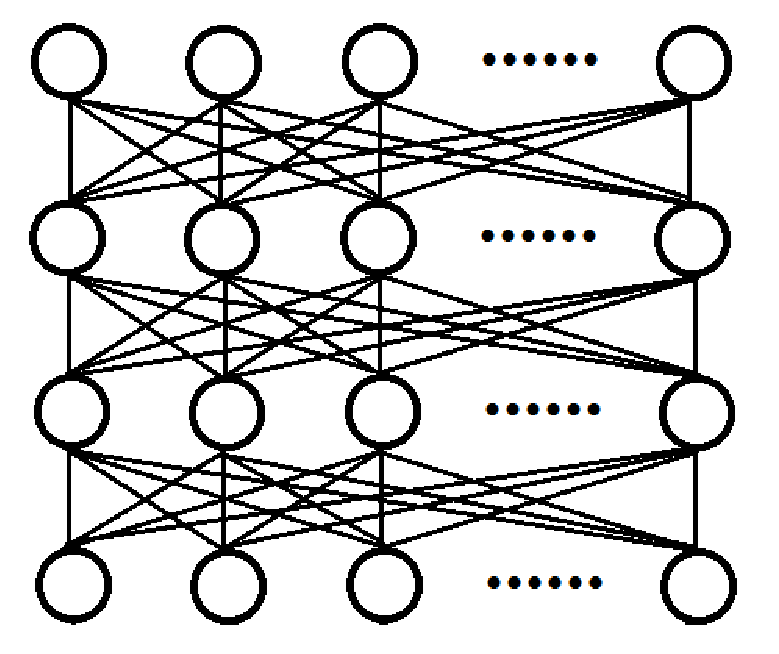
\includegraphics[width=0.35\textwidth]{DBN.eps}
\caption{DBN网络构型}
\label{img:DBN}
\end{figure}

我们之所以采用深度结构,是因为在神经元总数不变的前提下,深度结构的表达能力比浅结构的表达能力更强。之所以要在这个结构中引入受限玻尔兹曼机,是因为传统的深度结构无法训练。正如我们前面提及到的,深度结构会在网络的较浅层出现梯度消失现象,导致浅层无法对参数进行校正。由于数据必须从浅层神经元逐层地传播到深层神经元,一旦浅层的参数无法校正,将会导致深层的网络也无法进行参数校正,因为浅层参数无法校正意味着浅层无法对数据进行合理地重编码,数据经过浅层后得到的是混乱的数据,尽管深层不会产生太大的梯度消失现象,但数据经过浅层的打乱后,数据已经混乱了,训练也便没有意义。另一方面,传统的神经网络初始值设定为随机值,这些随机值一般设定为一个均值为0,方差较小的高斯分布,神经网络是一个非凸问题,局部最小值众多,网络最后收敛到的最小值取很大程度上决于初始值的选取,随机选取初始值虽然是一个可行的方法,但是如果我们能让参数的初始值设定在一个较合理的初始值,将会很大程度地改善网络的收敛性能,而受限玻尔兹曼机一个重要的贡献在于,将深度神经网络的参数初始化到一个较好的值。

深度置信网络的训练分为两个阶段,分别是预训练阶段和参数微调阶段。在DBN的预训练阶段中,将相邻两层看做一个受限玻尔兹曼机,采用受限玻尔兹曼机的训练方法,将原始数据作为最底层的输入,每层RBM隐含层的输出作为后一层的输入,然后进行逐层贪婪的无监督训练。对于每层RBM,其训练过程描述如算法\ref{alg:RBM} 所示

\vspace{1em}
\begin{minipage}{0.8\textwidth}\centering
\begin{algorithm}[H]\label{alg:RBM}
 \caption{受限玻尔兹曼机训练算法}
  \KwIn{由前一层网络提供的含有$n$个样本的数据集$S = \{x_i\}_{i=1}^n$;网络参数$w, b_h, b_v$; 动量项系数$p$;\\~~~~~~~~~~~~学习率$\eta$;权衰减系数$e$;CD-k中的参数$k$}
 \KwOut{训练好的网络参数;\\~~~~~~~~~~~~~~~由RBM提取到的数据$S' = \{y_i\}_{i=1}^n$}
\For{$i=1$;$i\leq1$; $i++$}
{
$v_0 = v_t = x_i$\\
$h_0$ = sampling h given v ($v_0$)\\
\For{$j=0$; $j < k$; $j++$}{
$h_t$ = sampling h given v ($v_t$)\\
$v_t $ = sampling v given h ($h_t$)\\
}
$\Delta_w = v_t^T * h_t - v_0^T * h_0$\\
$\Delta_{b_v} = v_t - v_0$\\
$\Delta_{b_h} = h_t - h_0$\\
$w = e * (p*w + \eta * \Delta_w)$\\
$b_v = b_v + \eta * \Delta_{b_v}$\\
$b_h = b_h + \eta * \Delta_{b_h}$\\
$y_i$ = sampling h given v ($x_i$)
}
\end{algorithm}
\end{minipage}
\vspace{1em}

算法中,学习率$\eta$、动量项系数$p$以及权衰减系数$e$我们将会留到网络设计技巧中讨论,这些技巧在数学推导的过程中是不必要的,然而在实际工程中是必要的,有时候缺了它们网络训练会失败。当逐层训练完毕后,网络的参数已经初始化到一个较好的位置\citeup{whyHelp}。在参数微调阶段,接着执行全局的反向传播算法进行有监督的权值微调。通过这样的方法,可以避免单纯地使用反向传播方法中会出现的陷入局部最优问题,由于识别的过程中,数据是逐层地进行维度变化,所以DBN也可以认为是一种特征提取方法,对应的,深度学习有时候也称之为“特征学习”\citeup{multipRespresen}。

\BiSection{本章小结}
x本章中,我们从传统的神经网络说起,介绍了神经元的工作原理以及神经网络的前向传播。当数据经过神经网络的逐层编码后,得到的编码并不是人类所能理解的编码,因此我们介绍了两种分类器将这些编码转换成自然语言所能描述的编码。随后我们介绍了神经网络的反向传播算法,最后引出深度置信网络。尽管这章名为“深度置信网络”,我们却对“深度置信网络”的介绍篇幅很短,但由于深度置信网络中并没有太多额外的东西,很多思想都是与传统神经网络是相同的,所以我们花了较大的篇幅取介绍传统神经网络。在本章中,我们依然留下一些问题没有解决,即训练过程中的一些额外参数,例如学习率、动量项等,关于这些内容,由于其更偏向于工程内容,我们将其集中到“神经网络设计技巧”章节中讨论。




\BiChapter{卷积神经网络}{CNN}
卷积神经网络灵感源自哺乳动物的视觉系统,它是唯一一个不需要预训练便能直接训练的深度网络。LeCun在1989年设计了第一个卷积神经网络,并将这个网络运用到邮编数字识别中取得了很好的效果,随后,xxxx将卷积神经网络应用到文档识别中,实现了可理解数字串的网络,这是一个重大的突破。但卷积神经网络在提出的二十多年里一直默默无闻,直到最近几年,人们发现在图像识别中卷积神经网络相比于其他的模型能更好地进行特征提取才被重视。目前,几乎所有最好的识别系统都是基于卷积神经网络的,从某种意义上而言,卷积神经网络相当于深度学习的代言人。
\BiSection{卷积神经网络综述}
x卷积神经网络可以看做是一种特殊的神经网络,在深度置信网络中,网络节点是全连接的,而卷积神经网络中连接是局部的。此外,卷积网络强制权值共享,对比于深度置信网络,卷积网络的这些特性都体现着非常强的正则。

\begin{figure}[htbp]
\centering
\subfigure{\label{img:fullNN2D}}\addtocounter{subfigure}{-2}
\subfigure{\subfigure[全连接神经网络]
			{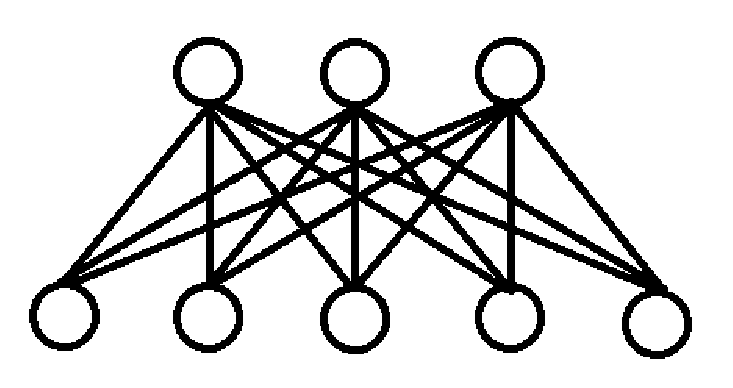
\includegraphics[width=0.4\textwidth]{CNN/fullNN2d.eps}}}
\subfigure{\label{img:conv2D}}\addtocounter{subfigure}{-2}
\subfigure{\subfigure[卷积神经网络]
			{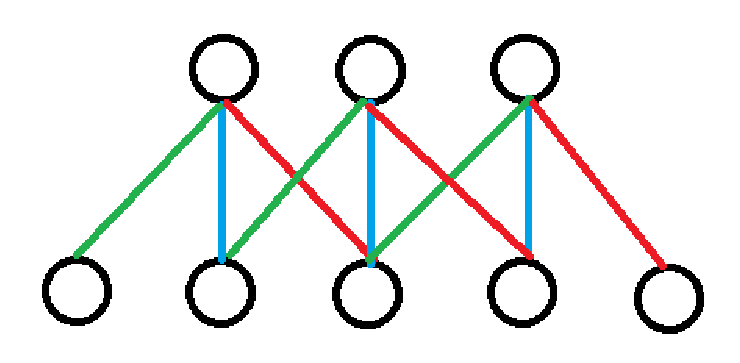
\includegraphics[width=0.4\textwidth]{CNN/convNN2d.eps}}}
\caption{二维视觉下的全连接神经网络与卷积神经网络}
\vspace{-1em}
\end{figure}

如图\ref{img:fullNN2D}所示为传统的全连接神经网络,我们可以看到,每一个上层节点与下层节点都含有连接,而所有的连接都是独立无关联的,即每个连接权值都不相等。对应的,图\ref{img:conv2D}所示为卷积神经网络,在这种网络构型中,每个上层节点只与部分的下层节点连接,并且,这些连接的权值是共享的,即相同颜色的连接代表其权值相等。局部连接将会大大减少网络的连接数量,而权值共享又会大大减少网络的参数数量。例如在图\ref{img:conv2D}中,连接数量为$3\times 5 = 15$,由于权值不共享,其参数数量也是15。而图\ref{img:conv2D}的连接数量为$3\times 3$,权值共享使得网络的参数只有3个。卷积网络的设计目的是让网络拥有更多的连接,而拥有更少的权值。尽管这里连接数量上卷积网络要比全连接网络少,但是我们后面将会看到,卷积网络将通过多张特征图构造出更多的连接。

卷积神经网络,一般用于图像识别与声音识别两个领域,因为这两个领域带着明显的二维特性。例如在图像识别中,图像即可以看做是高维的,也可以看做是二维的,如果将它看做高维的,那么就是将像素点展开成为一个高维列向量,展开后的图像将不再具有原始的面貌。如果将它看做是二维的,就是保留图像的原貌,利用二维的平面直角坐标系来描述。声音之所以可以看做二维的,是因为它带有时间这一维度,关于声音识别,我们不过多讨论,更多的细节请参考文献xxxx。

\begin{figure}[htbp]
\centering
\subfigure{\label{img:fullNN3D}}\addtocounter{subfigure}{-2}
\subfigure{\subfigure[全连接神经网络]
			{\includegraphics[width=0.4\textwidth]{CNN/fullNN3d.eps}}}
\subfigure{\label{img:convNN3D}}\addtocounter{subfigure}{-2}
\subfigure{\subfigure[卷积神经网络]
			{\includegraphics[width=0.4\textwidth]{CNN/convNN3d.eps}}}
\caption{三维视觉下的全连接神经网络与卷积神经网络}
\vspace{-1em}
\end{figure}

由于卷积网络保留了图像的二维面貌,因此相比于全连接神经网络而言,其网络构型是一个三维构型,如图\ref{img:fullNN3D}所示为三维视觉下全连接神经网络。由于上层节点是一个高维列向量,我们可以认为这个向量是一维的,并且这个向量里的每一个元素都与输入图像上的每一个像素点连接,不同元素之间的连接权值是不同的。而图\ref{img:convNN3D}所示是三维视觉下的卷积神经网络,我们可以看到,上层节点是一个二维矩阵,因此它的特征我们可以认为是二维的,这些上层节点组成的二维矩阵我们称为特征图(feature map),特征图里的每一个元素,都只与输入图像上的一小块区域有连接,并且,特征图里的不同元素的连接权值是相等,这些相同的连接权值我们称之为卷积核(convlution kernel)。图\ref{img:convNN3D}仅仅是一张特征图,实际中的卷积神经网络,往往通过多个不同的卷积核,卷积出多张特征图。

\BiSection{卷积神经网络的前馈}
x一个完整的卷积神经网络应包含三个内容:卷积层、采样层以及全连接层,关于各层的细节以及作用我们将在后面的小节中叙述,现在让我们先大致了解卷积神经网络的结构。如图\ref{img:CNN}所示是卷积神经网络其网络构型
\begin{figure}[!htbp]
\centering
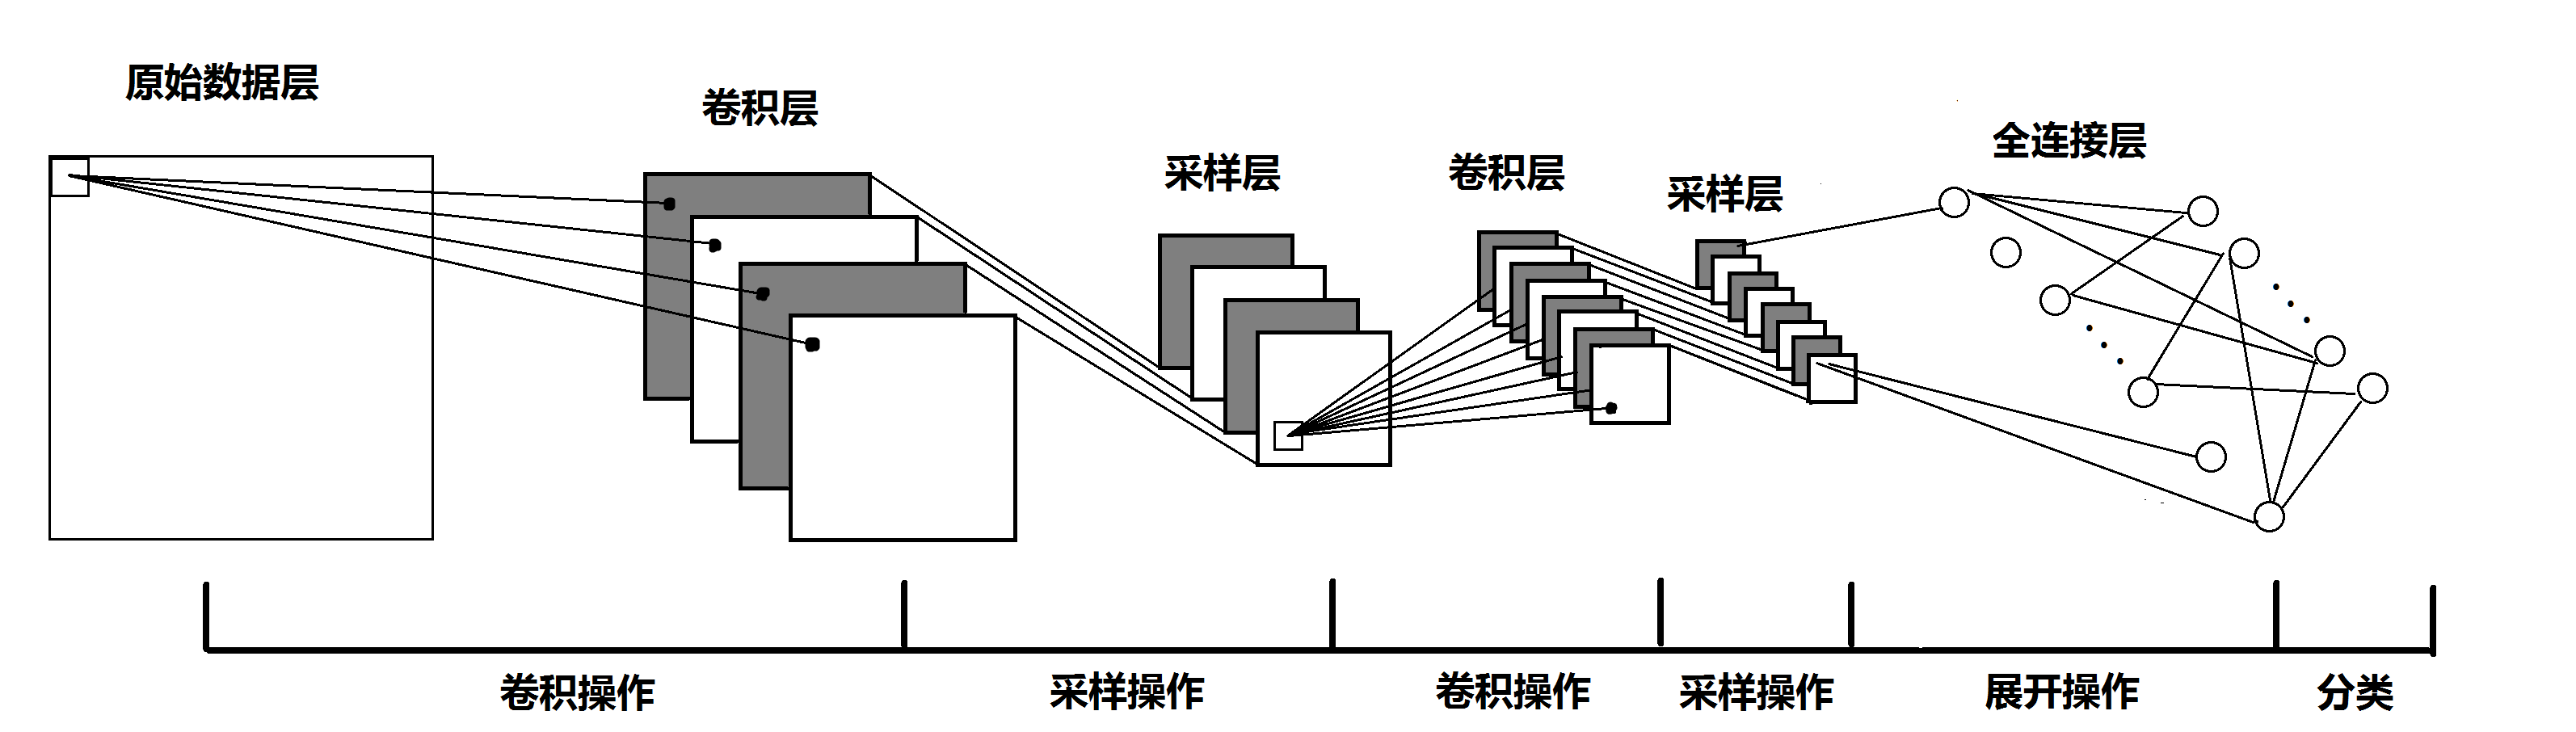
\includegraphics[width=0.8\textwidth]{CNN/CNN.eps}
\caption{卷积神经网络网络构型}
\label{img:CNN}
\end{figure}

在这种结构中,卷积层与采样层交错出现,在网络顶端采用全连接神经网络或其他分类器。图中卷积层里的每一张特征图,其执行过程都如图\ref{img:convNN3D}所示,这些不同的特征图对应着不同的卷积核,多张特征图,增加了网络的连接数目,但由于每张特征图只对应一个卷积核,所以网络的参数(即卷积核)的数目相比与全连接神经网络参数的数目而言是很小的。

\BiSubsection{卷积}
x卷积神经网络所使用的卷积即二维离散卷积,其定义为
\begin{equation}
\begin{split}
y[s, t] &= \sum\limits_{i=1}^{m_1 +  m_2 -1}\sum \limits_{j=1}^{n_1 + n_2 -1} x[i, j]\cdot k[s-i+1, t-j+1]\\
&~~~~~~~ 1\leq s \leq m_1 + m_2 -1\\
&~~~~~~~ 1\leq t  \leq n_1  + n_2 - 1
\end{split}
\end{equation}

式中,$x$为$m_1\times n_1$的矩阵,称为原始数据,$x[i,j]$代表$x$中的第$i$行第$j$列元素。$k$为$m_2 \times n_2$的矩阵,称为卷积核,$k[i, j]$代表$k$中的第$i$行第$j$列元素。$y$为$(m_1 + m_2 -1)\times (n_1 + n_2 -1)$的矩阵,称为卷积结果,$y[i, j]$代表$y$中的第$i$行第$j$列元素。如果从图像上来解释二维离散卷积,卷积层的操作相当于图\ref{img:convlution}所描述的过程。图中,原始图像是一张$5\times 5$像素的数字“4”的二值图像,如果我们定义卷积核为
\begin{equation}
kernel = \left[
\begin{array}{ccc}
~0~&~~~0~~~&~0~\\
~0~&~~~2~~~&~0~\\
~0~&~~~0~~~&~0~
\end{array}
\right]\label{equ:kernel}
\end{equation}

\begin{figure}[!htbp]
\centering
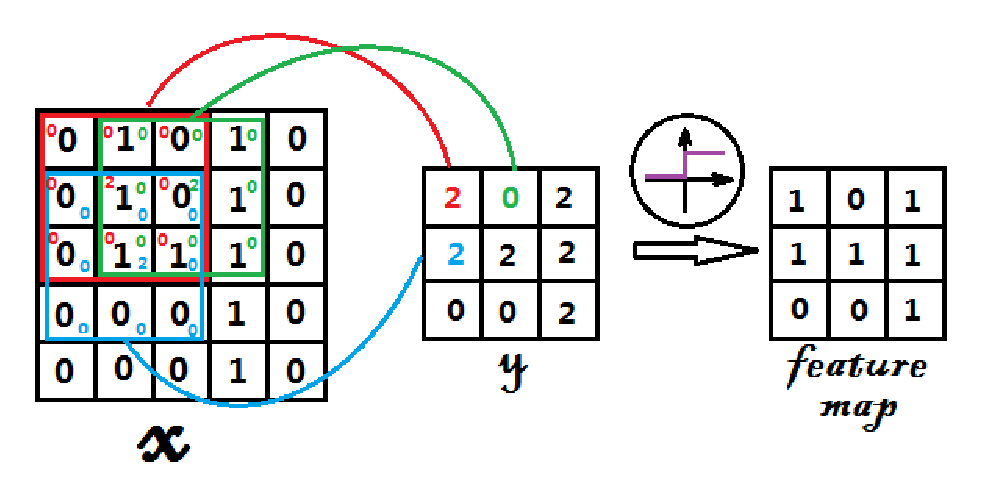
\includegraphics[width=0.8\textwidth]{CNN/convlution.eps}
\caption{卷积神经网络网络构型}
\label{img:convlution}
\end{figure}

那么经过二维离散卷积后,其得到的卷积结果为
\begin{equation}
y = x * kernel = 
\left[
\begin{array}{ccc}
~2~&~~~0~~~&~2~\\
~2~&~~~2~~~&~2~\\
~0~&~~~0~~~&~2~
\end{array}
\right]
\end{equation}
将卷积结果再经过一个阶跃函数进行非线性变换后,我们可以看到,卷积层通过式\eqref{equ:kernel}中定义的卷积核对原始图像(即数字4)进行卷积后,其非线性化后的结果依然保留着数字4的特征。由于卷积核是固定的,因此卷积操作经常被认为是一种滤波,即用卷积核去检测特征,将这些特征提取出来。

图\ref{img:convlution}只是利用一个卷积核对原始图片进行卷积得到一张特征图,事实上,正如图\ref{img:CNN}所示,如果我们利用多个卷积核对原始图像进行卷积,那么便可以得到多张特征图。多张特征图,意味着可以提取到原始图像的多个特征,例如在手写数字识别中,我们提取了三张特征图,其中一张特征图表明左上角有一点,一张特征图表明右上角有一个折线,剩下的一张特征图表明右下角有一个点,那么通过这三张特征图,我们就可以判定这个数字是“7”。特征图的作用,在于降低数据的冗余信息,例如“7”这个数字中,横线事实上只需要两个点就可以确定一条直线,竖线也同理只需要两点便可确定一条直线,然而横线与竖线之间存在一个相对位移,因此折线的作用便是刻画相对位移的。

图\ref{img:convlution}中的例子只针对与原始输入数据是一张图像的情况,实际上,卷积操作应该泛化到输入图像为多张的情况。例如,图图\ref{img:CNN}中的第二个卷积层,其输入图像便是多张图像。实际中,输入图像也不太可能是一张图像,一张输入图像的情况往往只出现于灰度图像中。然而在彩色图像中,我们知道,彩色图像是具有三张矩阵的,分别代表红(R)、绿(G)、蓝(B)。对于输入图像为多张的情况,解决的方法有两种。一种是利用同一个卷积核去卷积所有的$n$输入图像,将得到的$n$张卷积结果进行相加合并成为一张,在将它进行非线性映射,从而得到一张特征图,这个过程如图\ref{img:convlution4featuremap}所示。

\begin{figure}[!htbp]
\centering
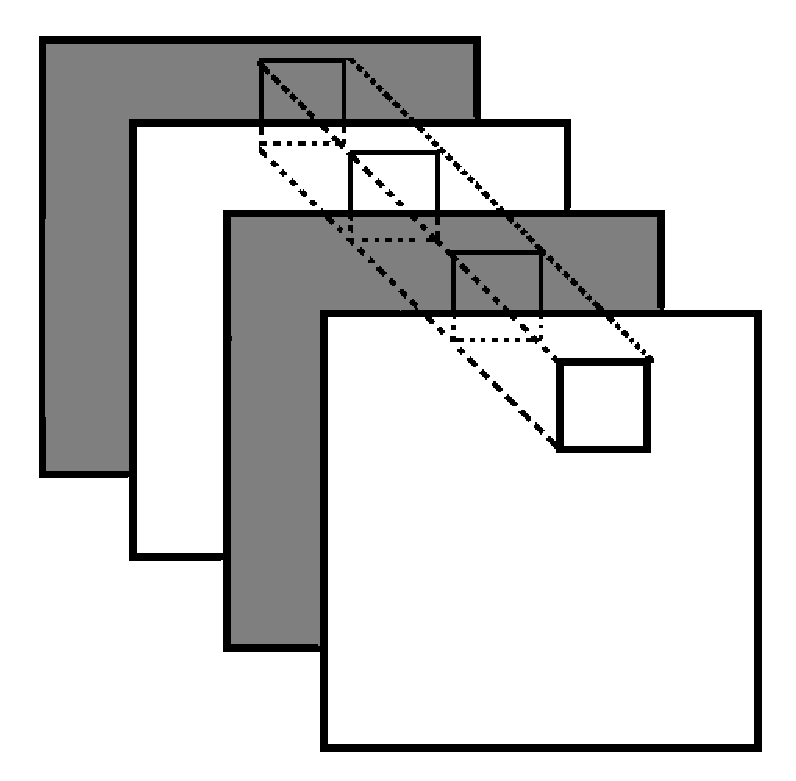
\includegraphics[width=0.3\textwidth]{CNN/convlution4featuremap.eps}
\caption{使用同一卷积核卷积多张图像}
\label{img:convlution4featuremap}
\end{figure}

另外一种解决方法是,假设我们有$ m $张输入特征图,而我们想要卷积后得到$ n $ 张输出特征图,那么我们使用 $m \times n$ 个卷积核,令$ k_{i,j}$ 代表从第$ i $张输入特征图映射到第$ j $张输出特征图这个过程中所需要使用的卷积核,$ b_j $代表卷积完成后第$  j $张特征图所要加上的偏置,那么卷积操作就可以描述为:
\begin{equation}
\bigg[\mathcal{M}_1, \mathcal{M}_2, \cdots, \mathcal{M}_m\bigg] \divideontimes \left[
\begin{array}{cccc}
k_{1,1} & k_{1, 2}, & \cdots, & k_{1, n} \\
k_{2,1} & k_{2, 2}, & \cdots, & k_{2, n} \\
\vdots &\vdots & \ddots  & \vdots \\
k_{m,1} & k_{m, 2}, & \cdots, & k_{m, n} \\
\end{array}
\right ] \boxplus \bigg[b_1, b_2, \cdots, b_n\bigg] = \bigg[\mathbf{M}_1,\mathbf{M}_2, \cdots, \mathbf{M}_n\bigg]
\label{equ:muticonv}
\end{equation}
式中,$\big\{\mathcal{M}_i\big\}_{i=1}^m$为$m$张输入特征图,$\big\{\mathbf{M}_j\big\}_{j=1}^n$为$ n $张输出卷积结果, $\boxplus$为面向元素的加法,$\divideontimes $是我们提出的一种运算,其运算与矩阵乘法类似,唯一不同是在元素操作时,矩阵乘法执行的是乘法操作, 而$\divideontimes $执行的是卷积操作。卷积操作完成后,再进行非线性映射,即可得到多张特征图。式\eqref{equ:muticonv}实际上类似于全连接神经网络的前向传播,但是不同的是,全连接神经网络中,$m \times n$矩阵里的每一个元素代表连接权值,是一个常数,而式\eqref{equ:muticonv}中,$m \times n$矩阵里的每一个元素代表一个卷积核,是一个矩阵。另外一个不同点在于,全连接神经网络执行的是乘法,而式\eqref{equ:muticonv}中执行的是卷积。

事实上,第一种解决方案只是第二中解决方案的特例,在第一种解决方案中,实际上相当于$K_{m \times n}$中的每一列都强制相等,即
\begin{equation}
k_{1, 1} = k_{2, 1} = \cdots = k_{m, 1}
\end{equation}
因此,第一种解决方案意味着更强的正则,或者说更强的惩罚,因为它强制每一列的卷积核都相等。但是我个人认为,尽管这种方法确实能工作得很好,但这是不太合理的。例如在图像中,三个输入图像,也就是RGB三个矩阵,采用第一种方案意味着对三个颜色都同等对待,因为作用在三个矩阵上的卷积核是相同的。但我们直觉上可以感觉到,这三种颜色不应该同等对待,而应区分开来,因此在往后的讨论中,我们只讨论第二种解决方案。

\BiSubsection{采样}
x卷积得到的特征图,需要经过一个采样层,采样层是针对每一张特征图的,即各张特征图的采样时独立互不干扰的,因此采样得到的特征图与原始的特征图之间是一一对应关系。假设我们使用一个均值采样,对于一个$4\times 4$的特征图,我们对其每$2\times 2$区域内取平均,即

\begin{equation}
\left[
\begin{array}{cccc}
1 &~~~~1 &~~~~2& ~~~~2\\
1 &~~~~1 &~~~~2& ~~~~2\\
3 &~~~~3 &~~~~4 &~~~~4\\
3 &~~~~3 &~~~~4 &~~~~4\\
\end{array}
\right] \rightarrow \left[
\begin{array}{cc}
1&~~2\\
3&~~4\\
\end{array}
\right]
\end{equation}

采样层的作用在于压缩数据,使得维度不至于快速增长。想象一个原本为$6\times 6$像素的原始图片,在经过一个$3\times 3$的卷积核进行卷积后,得到的特征图大小为$4\times 4$,但这只是一张特征图,由于在卷积层中我们往往使用多个卷积核进行卷积,假设我们设定卷积层的输出特征图总量为50,那么将会有$50\times 4 \times 4 = 800$个节点,而原来的节点只有$5\times 5 = 25$个节点,这将会使节点增加了32倍。采样层一般都是对卷积得到的特征图进行2倍的缩小,仅此经过采样层后,特征图的大小为$2\times 2$,此时的节点仅为$50\times 2 \times 2 = 200$个。

另一方面,采样层可以抑制位移的变化,卷积得到的特征图,在经过小区域内的平均后,弱化了其绝对位置,而保留了其相对位置,需要注意的是,这里的位移并不仅仅只欧式距离里的位移,还应包括图像的伸缩,旋转等,所以这个位移应理解为广义的位移。

采样的方法除了上面提到的平均采样方案,还有一些别的方案,例如xxx文献中介绍了一种自学习的采样,即小区域内并不是简单的求和取平均,而是类似于加权求和取平均,这些权值便是所需要学习的参数。这两种方案并没有孰劣孰优的说法,实际上两者都能很好的工作,但自学习的方法确实是会比简单的平均采样好一些,但由于平均采样更简单,所以我们往后的讨论只使用平均采样。

\BiSubsection{分类器}
x原始输入数据经过多次卷积采样后,特征图的尺寸不断缩小,最后将使得卷积无法再进行,此时,我们将这些非常小的特征图展开成为一个列向量。例如,一个原始图片为$32\times 32$大小的图像,经过一个$5\times 5$大小的卷积核后得到$28\times 28$的特征图,对其进行均值采样,将变为$14\times 14$大小的特征图,再用$5\times 5$大小的卷积核卷积,将得到$10\times 10$大小的特征图,采样后为$5\times 5$大小,此时再执行一次卷积后,特征图大小为$1\times 1$,这时候再也无法进行采样了,假设现在有100个$1\times 1$大小的特征图,那么它便可以展开成为一个100维的列向量。又例如,一个原始图片为$28\times 28$大小的图像,如果卷积核都设定为$5\times 5$,那么经过卷积、采样、卷积、采样后,将得到$4\times 4$的特征图,此时卷积核尺寸大于特征图的尺寸,卷积无法执行,应将这些特征图展开,假设有10张$4\times 4$的特征图,那么展开后将得到$10 \times 4 \times 4 = 160$维的列向量。

对于最后的列向量,即可以直接使用分类器,也可以在这些列向量的基础上搭建几层隐含层后再使用分类器,这个分类器可以是全连接神经网络或支撑向量机等,选取哪个取决于设计者的意愿。关于分类器如何使用,读者可以参考前面的章节,在卷积网络最顶层的分类器中,与传统神经网络是相同的。

\BiSection{卷积神经网络的反馈}
x卷积神经网络的训练方法与传统神经网络的训练方法类似,都是采用反向传播算法,但由于卷积网络特殊的构型,需要对其进行一些改动,但两者的核心都是相同的,即通过后一层的误差注入前一层中,乘上该层激活函数相对于净激活的偏导数后得到该层的误差,利用这个误差乘上净激活相对于输入的偏导数即可得到参数更新的增量。唯一的不同点在于注入的方式不同。
\BiSubsection{分类器误差传播}
x由于卷积神经网络中最顶层与传统的神经网络相同,因此参数校正以及反向传播方式是相同的。有一点需要注意的是,如果网络最后一个卷积层(或采样层)中将特征图拉成一个列向量,那么反向传播的时候需要将列向量还原回特征图形式,例如,如果网络中最后阶段得到10张$4\times 4$大小的特征图,前向传播过程中会将它们合并成为一个160维的列向量,那么在反向传播过程中,需要将160维的误差列向量还原成10张$4\times 4$的特征图形式,此时得到的特征图可以看做是误差特征图。
\BiSubsection{采样层误差传播}
x在采样层中,如果我们使用平均采样,由于平均采样并没有额外的参数需要学习,因此只需要将后一层传播回来的误差继续传播回前一层即可。由于采样层是对前一层局部区域的平均,所以在将误差传播回前一层时,只需要将其尺寸放大到相同的比例,对应的局部区域中每一个元素均取采样层中的元素即可。例如,一个缩小比例为2的采样层,假设它接收到后一层传播回来的误差特征图尺寸为$2\times 2$,那么这个误差传播回采样层的前一层将得到$4\times 4$尺寸的特征图,这个过程如式\eqref{equ:subsampling}所示
\begin{equation}
\left[
\begin{array}{cc}
1&~~2\\
3&~~4\\
\end{array}
\right]\rightarrow 
\left[
\begin{array}{cccc}
1 &~~~~1 &~~~~2& ~~~~2\\
1 &~~~~1 &~~~~2& ~~~~2\\
3 &~~~~3 &~~~~4 &~~~~4\\
3 &~~~~3 &~~~~4 &~~~~4\\
\end{array}
\right] \label{equ:subsampling}
\end{equation}

如果读者在此之前了解过Kronecker积(也称直积),上述过程便是一个Kronecker积过程,即

\begin{equation}
\delta_{conv} = \delta_{sampling} \otimes 1_{n \times n}
\end{equation}
式中需要注意的是,$\otimes$是直积符号而不是逻辑电路里的异或符号。$\delta_{conv}$代表传播回前一层(即卷积层)的误差,$\delta_{sampling} $代表后一层网络传播到采样层的误差,$1_{n \times n}$是一个$n \times n$的单位向量,$n$的取值等于采样层的缩小比例,例如,如果采样层的缩小比例是2,则$n=2$。

\BiSubsection{卷积层误差传播}
x与传统的全连接神经网络类似,卷积层接收到后一层传播回来的误差后,需要乘以当前层激活函数相对于净激活的偏导数,得到当前层的误差,即
\begin{equation}
\delta^\ell_i = \delta^{\ell + 1}_i \cdot \frac{\partial f(net_i)}{\partial net_i}
\end{equation}
由于卷积网络中有多张特征图,所以$\delta^\ell_i $代表当前层($\ell$层)的第$i$张误差特征图,$\delta^{\ell + 1}_i$代表第$\ell + 1$层传播回来的第$i$张误差特征图,$net_i$代表第$i$张特征图的净激活。

计算得到当前层的误差后,通过卷积的自相关性,利用这个误差可以计算卷积核以及偏置的迭代增量,即\citeup{bouvrie2006notes}
\begin{equation}
\frac{\partial J}{\partial k_{i, j}^\ell} =rot180\bigg(conv\Big(x_i^{\ell-1}, rot180(\delta_j^\ell),'valid' \Big)\bigg) 
\end{equation}
式中,$rot180( \cdot )$执行将一个矩阵旋转$180^\circ$操作,其目的在于利用卷积的自相关性质,conv为卷积操作,‘valid’代表卷积操作范围限制在可用区域内。对于偏置,其梯度为\citeup{bouvrie2006notes}
\begin{equation}
\frac{\partial J}{\partial b_j} = \sum\limits_{u, v} (\delta_j^\ell)_{uv}
\end{equation}
获取参数的梯度后,对卷积层的参数进行更新,随后将卷积层的误差反向传播到采样层,其公式为\citeup{bouvrie2006notes}
\begin{equation}
\delta_j^{\ell -1} = f'(u_j^\ell) \boxdot conv\bigg(\delta_j^\ell, rot180\Big(\sum\limits_{i\in M_j^\ell} k_{ij}^\ell\Big), 'full' \bigg)
\end{equation}
式中,$\boxdot$为面向元素的乘法,‘full’代表卷积的操作范围是全图卷积。通过以上策略,对网络进行类似的反向传播,即可对整个网络进行反馈校正。



\BiSection{本章小结}
x本章中我们介绍了卷积神经网络中卷积层以及采样层的原理,并介绍了一种卷积神经网络的结构。卷积网络的结构变体有很多,1989年LeCun设计的第一个卷积神经网络仍带有轻微的全连接网络气息\citeup{lecun1989backpropagation},而1998年LeCun与Bengio等人设计的卷积神经网络在卷积时并不是全特征图卷积,而是选取一部分的特征图进行卷积\citeup{lecun1998gradient}。Lee Honglak与Andrew Ng等人将受限玻尔兹曼机与卷积神经网络相结合,形成一种名为Convolutional deep belief networks的神经网络\citeup{lee2009convolutional}。文献\cite{krizhevsky2012imagenet}中介绍了一种使用三维卷积核的卷积网络,因此这种网络可以看做是四维网络,Krizhevsky等人利用它在2012年的ImageNet LSVRC-2010数据集上获得了世界第一的正确率,这种卷积网络成为当前的主流结构。尽管卷积网络的变体众多,但其大体思路是类似的,都是基于卷积核对局部特征进行提取。







\BiChapter{神经网络的设计技巧}{trick}
神经网络的设计技巧众多,这些技巧大致可分为两大类,一类是训练前对数据的预处理,另一类是训练过程中采用的一些特殊的训练手段。数据预处理的作用在于将原始数据处理成容易训练的数据,加快准则函数的收敛速度,另一方面,原始数据的降维可以在牺牲较小精度的前提下减少运算量,提高程序的执行效率。训练过程中采用的一些特殊手段在数学上是没有太大意义,甚至有时候是违反直觉的,这些技巧是多年来科研人员积累出来的经验,其灵感来源一般靠蒙。尽管这些经验有时候反而会降低网络的性能,但大部分情况下确实会提高性能的,某些情况下,不适用这些技巧,网络的训练初始阶段准则函数无法收敛。具体设计过程中,对于这些技巧,我们应该抱着试一试的心态,如果在网络中使用某个技巧,使得网络性能变好了,那么我们便保留这个技巧,否则如果网络性能变差了,那么就舍弃这个技巧\footnote{但前提是这个技巧被正确使用,即编码正确}。
\BiSection{数据预处理}
x数据的预处理大致可分为几类:白化、降维、扩容、归一化。白化的作用在于去除数据耦合的相关性,降维的作用在于压缩数据,加快算法执行效率,由于主成分分析是一种去除相关性的降维方法,因此我们将白化合并到主成分分析的章节中而不另起章节。扩容目的在于利用一些手段,人工地伪造一些训练数据,将训练样本的容量扩大,使得网络的泛化能力变强。归一化的目的在于让数据保持在$[0,1]$区间内,之所以要在这个区间内,一方面,在一些激活函数,比如Sigmoid函数中,如果数据尺度过大,则使得激活函数迅速饱和,从而梯度接近于0,权值更新缓慢。而数据归一化到较小的数值上时,我们知道,Sigmoid函数在原点附近是一个近似于线性的函数,在训练的初始阶段便可让权值获得较大的梯度。另一方面,如果数据尺度过大,有可能会导致计算机的数值溢出,尤其是激活函数为Sigmoid的时候,因为这个激活函数带有一个指数项,对于某些不自带溢出检测的编程语言如C++而言,这是一场灾难,因为它会导致你的代码莫名其妙地失败。即使是一些带溢出检测的语言,如Python,当数值溢出时,往往使用Inf或NaN代替,此时进行的不再是数值运算,而是符号运算,这将极大地降低运算速度。
\BiSubsection{降维}
x人是一种受限于三维空间的动物,我们只能理解三维的而无法想象更高维度的事物。事实上,人同样无法理解二维的或一维的世界,尽管我们可以在脑海中想象二维曲面或一维曲线,但人脑海里的这些事物这些都不是二维,他们只是嵌在三维空间中的二维(或一维)流形\footnote{更多有意思的观点可以观看麻省理工学院的《量子力学》公开课}。一张一百万像素的图片,它总能对应着一百万维空间中的某一点,而很多张某个类比的图片,比如狗的图片,将会对应着一百万维空间中的多个点。然而并不是一百万维空间中的任何一点都是狗的图片,它也有可能是猫的图片,但是同样是狗的图片,它会在总会有某些共通性,这些共通性,或者说特征,使得狗这一类图片在一百万维的空间中构成一个流形,如果我们能找到这个流形,那么我们就可以避开一百万维空间,直接在低维流形中进行分类。

由于我们无法理解高维空间,因此我们通过一个三维空间中的二维流形简单叙述这件事,如果我们通过式\eqref{equ:xyzpoint}求取三维空间中任何一点的$(x, y, z)$坐标
\begin{equation}
\alpha = 1.5\pi *(1+2 * random)
\end{equation}
\begin{equation}
x = \alpha * \cos\alpha~~~~~~~~y = 21 * random~~~~~~~~z = \alpha * \sin\alpha
\label{equ:xyzpoint}
\end{equation}
式中,$random$是$[0,1]$区间内均匀分布的随机数,那么我们就可以得到一个称为“swiss roll”的散点图,如图\ref{img:swiss roll}所示
\begin{figure}[!htbp]
\centering
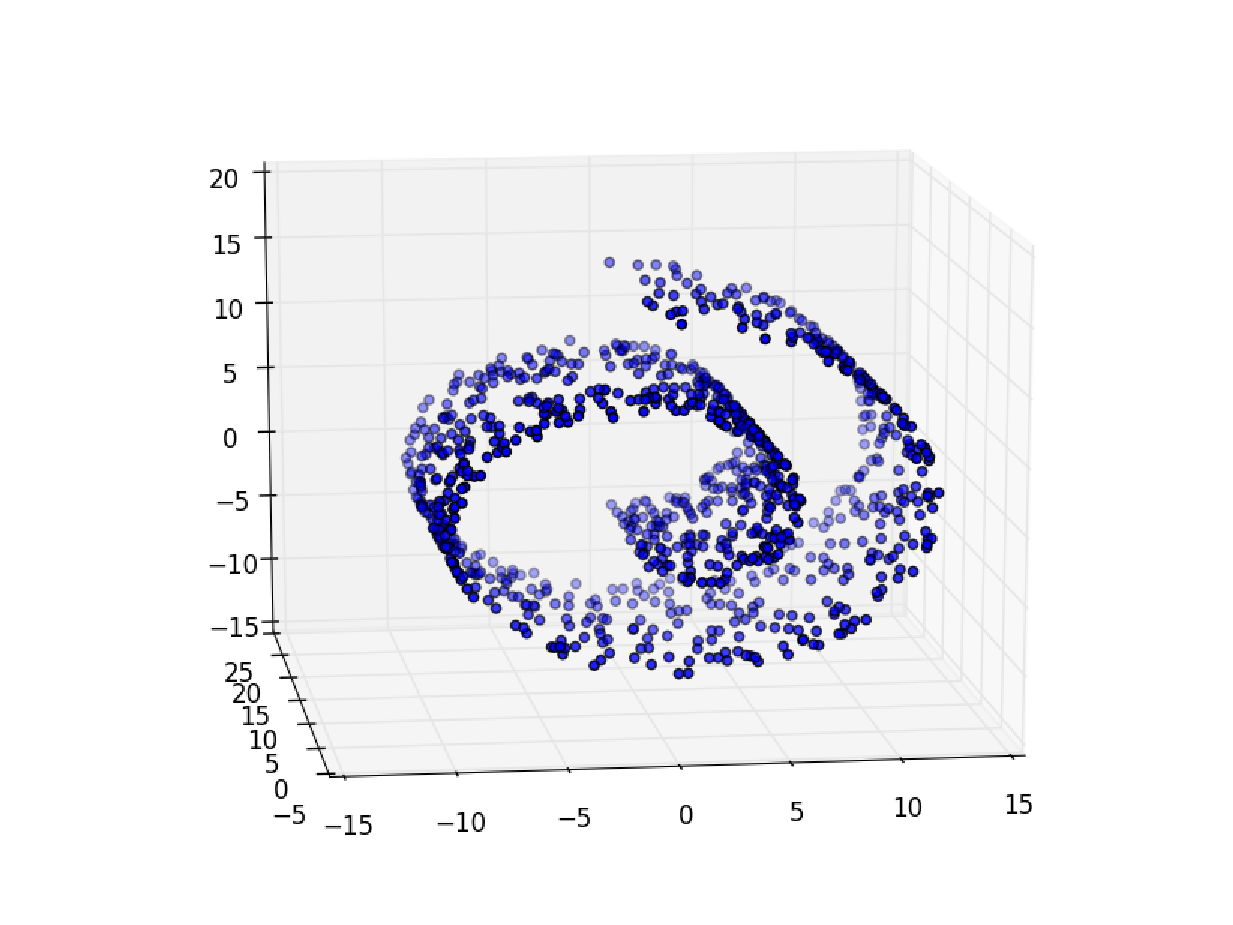
\includegraphics[width=0.8\textwidth]{trick/swissRoll.eps}
\caption{Swiss Roll}
\label{img:swiss roll}
\end{figure}
如果这些点分别代表一个三维的数据样本,那么我们可以发现,这些样本坐落于一个二维流形中,即图\ref{img:swiss roll}中卷筒蛋糕的形状。这里我们用了错误的措辞,因为流形实际上是一个空间而不是一个形状,但为了通俗地解释这件事,我们认为采用这种措辞是可取的。观察式\eqref{equ:xyzpoint},我们可以发现,事实上三维空间中的点$(x,y,z)$可以只用二维空间的$(\alpha, y)$描述,因为$x$和$z$都是$\alpha$的函数,从图像上我们也可以直观的感受到,三维数据是多余的,因为数据的坐落位置十分有规律。

降维,也是同样的思想,高维的数据是带有冗余的,如果我们能找到这些数据的低维流形,那么就可以在低维空间中进行数据处理。这衍生出了机器学习的一个流派---流形学习。关于流形学习我们不会做过多的介绍,我们只在本章中介绍两种降维方法,即主成分分析和多维尺度分析。与统计学习类似,实际中我们也无法找到数据真实的低维流形,不同的降维方法相当于对低维流形的不同逼近方法。如果说数据背后确实存在一个低维流形,而我们的降维方法又恰好是这个流形的描述,那么降维不会引入信息的损失,例如,三维坐标降到球坐标并不会引入误差,但实际中我们我们并不知道具体流形,我们的降维方法也不是真实的维度变换方法,所以实际中的降维一定会引入信息的损失,导致分类性能的下降,相比于降维带来的巨大好处----运算效率的提高,这个性能的下降是可接受的。图像识别,由于生活图像其维度都以千万记,降维是必须的,否则以目前的计算机性能无法完成准则函数的收敛。

\BiSubsubsection{主成分分析}
x为了简单起见,我们只在这里讨论如何使用主成分分析将二维空间中的数据降到一维空间,但二维空间中的结论很容易被推广到更高维度的情况,因为更高维度空间中的结论与二维空间中的结论是相同的。

假设我们有一个含有$n$个$2$维样本的数据集$X = [x^{(1)}, x^{(2)}, \cdots, x^{(n)}]^T$,如图\ref{img:PCA dot}所示是一个含有100个样本的数据集在平面直角坐标系上的分布。

\begin{figure}[!htbp]
\centering
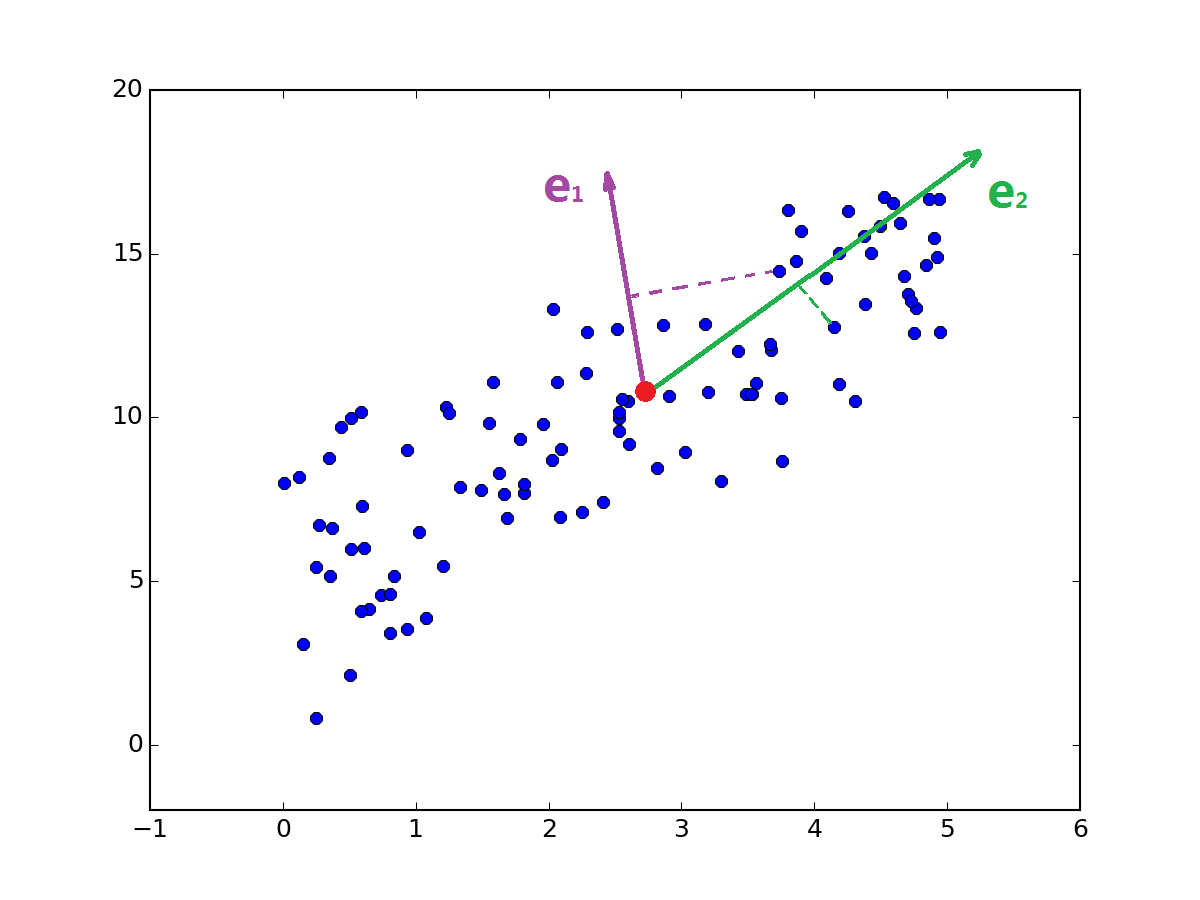
\includegraphics[width=0.5\textwidth]{trick/PCA_dot.eps}
\caption{二维空间中的数据样本点}
\label{img:PCA dot}
\end{figure}

如果我们通过计算得到这些样本点的均值$\bar{x}$,即
\begin{equation}
\bar{x} = \frac{1}{n}\sum\limits_{i=1}^n x^{(i)}
\end{equation}
正如图\ref{img:PCA dot}中的红点,那么我们总能将所有的点用一组基的线性组合来代替,即
\begin{equation}
x^{(i)} = \bar{x} + \alpha_1 e_1 + \alpha_2 e_2
\end{equation}
式中,$e_1$和$e_2$是任意两个不平行的单位向量,正如图\ref{img:PCA dot}中的紫色方向和绿色方向。但此时我们只是将样本点从一个原始的正交二维坐标系转换到另一个以$e_1$和$e_2$为基的二维坐标系,为了降维,我们必然需要舍弃一个维度,这个维度可能是$e_1$或$e_2$,然而选取哪个维度更好呢?直觉上我们会认为选取$e_2$会更好,因为当所有的数据点都投影到这个基上时,相比于$e_1$能更好地保留数据的信息。

然而,$e_1$和$e_2$是我们任意选取的两个基向量,事实上有可能有另外的基向量要比$e_1$更好的保留原始数据的特征,假设最优的基向量为$e$,那么为了刻画数据降维后原始数据与降维后数据的差异性,我们引入一个准则函数
\begin{equation}
J(\alpha_1, \alpha_2, \cdots, \alpha_n) = \sum\limits_{i=1}^n \bigg((\bar{x}+\alpha_i e) - x^{(i)}\bigg)\bigg((\bar{x}+\alpha_i e) - x^{(i)}\bigg)^T
\label{equ:PCA J}
\end{equation}
式中,$\bar{x}+\alpha_i e$实质上代表的是原始数据降维到一维空间后在二维空间中的坐标,即原始数据在基向量$e$的投影点的二维坐标。准则函数使用的依然是我们非常熟悉的二范数,这个准则函数事实上刻画的是原始坐标到投影坐标距离的平方,也就是两者究竟相差了多远。为了最小化这个准则函数,我们先对式\eqref{equ:PCA J}进行展开,这将得到
\begin{equation}
J(\alpha_1, \alpha_2, \cdots, \alpha_n, e) = \sum\limits_{i=1}^n \alpha_i^2 ||e||^2 - 2\sum\limits_{i=1}^n \alpha_i e^T(x_i - \bar{x}) + \sum\limits_{i=1}^n ||x_i - \bar{x}||^2
\end{equation}
由于$\sum_{i=1}^n ||x_i - \bar{x}||^2$只与数据相关而与参数无关可以舍去,此外,$e$是单位向量,所以$||e||^2$等于1,因此准则函数可以简写为
\begin{equation}
J(\alpha_1, \alpha_2, \cdots, \alpha_n, e) = \sum\limits_{i=1}^n \alpha_i^2  - 2\sum\limits_{i=1}^n \alpha_i e^T(x_i - \bar{x})
\label{equ:8.yyyy}
\end{equation}
为了最小化这个准则函数,我们对其求偏导,并另导数为0,则
\begin{equation}
\frac{\partial}{\partial \alpha_i} = 2\alpha_i - 2e^T(x_i - \bar{x}) = 0
\label{equ:8.xxxxxxx}
\end{equation}
因此当$\alpha_i = e^T(x_i - \hat{x})$准则函数取得最小。这实质上说明,当数据点投影到$e$时使得准则函数最小,与我们前面的猜测符合。将\eqref{equ:8.xxxxxxx}代回\eqref{equ:8.yyyy},我们便可以消去准则函数中的$n$个变量$\alpha_1, \cdots, \alpha_n$,只剩余一个变量$e$,即
\begin{equation}
J(e) = - \sum\limits_{i=1}^n e^T(x_i - \hat{x})(x_i - \hat{x})^Te
\end{equation}
如果我们记号散布矩阵为
\begin{equation}
S =\sum\limits_{i=1}^n (x_i - \hat{x})(x_i - \hat{x})^T
\end{equation}
则准则函数可以谢伟
\begin{equation}
J(e) =  -  e^TSe
\end{equation}
此时是一个约束优化问题,约束条件为等式约束$e^Te = 1$,为此引入拉格朗日乘子$\lambda$,构造拉格朗日函数为
\begin{equation}
\mathcal{L}(e) = - e^TSe + \lambda(e^Te-1)
\end{equation}
对拉格朗日求偏导,并另偏导为0
\begin{equation}
\frac{\partial}{\partial e} \mathcal{L}(e) = -2Se + 2\lambda e = 0
\end{equation}
此时说明,当$Se = \lambda e$时,准则函数最小,而事实上这是矩阵对特征根的定义,因此为了最小化准则函数,基向量$e$应当选取为散布矩阵$S$的特征向量。这个结论可以很容易推广到高维情况,假设我们有n个d维的数据样本,那么我们总能构造他的散布矩阵$S$,为了将它降到$k$维而同时又要使得准则函数最小化,我们应该选取$S$最大的$k$个特征值所对应的特征向量作为投影基,从而新的$k$维坐标为
\begin{equation}
\alpha_i = e^T(x^{(i)} - \hat{x})
\end{equation}

由于特征向量之间是正交的,因此降维后的数据在各个维度是独立的,这也是白化的目的,因此主成分分析也是一种白化方法。有时候我们需要将降维后的数据还原回原始的维度以检测降维后的数据究竟损失了所烧信息,那么利用特征向量的正交性,有
\begin{equation}
e\alpha_i = ee^T(x^{(i)} - \hat{x}) = x^{(i)} - \hat{x}
\end{equation}
此时等号两边同时加上均值$\hat{x}$即可还原出$d$维数据。如图\ref{img:PCA reconstruct}所示是$28\times 28$像素的图像,它共有784维,其原始数据为黑底的图像所示。如果我们使用主成分分析将其降到20维后再将其还原成784维数据,其图像如灰底图像所示,我们可以看到,经过降维后再还原的数据已经变得模糊化,而这些模糊化并不会影响我们对数字的识别。

\begin{figure}[!htbp]
\centering
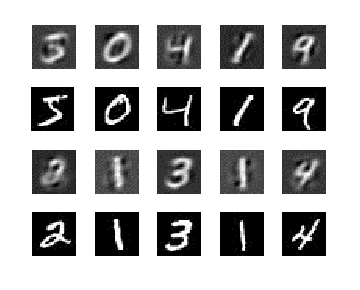
\includegraphics[width=0.3\textwidth]{trick/PCA.eps}
\caption{经过主成分分析降维后还原的数据}
\label{img:PCA reconstruct}
\end{figure}


\BiSubsubsection{多维尺度分析}
x在介绍多维尺度分析\citeup{kruskal1964multidimensional}之前,我们先从地图重构的问题讲起。假设我们在中国地图中选取五个城市,分别为北京、上海、广州、兰州、哈尔滨,依次用A、B、C、D、E代替。如果我们以北京为坐标平面的原点,那么剩下的城市坐标分别为:上海$(631.6, -796.4)$、广州$(103.8, -2029.2)$、兰州$(-1228, -428.1)$、哈尔滨$(265, 1082)$,将这些城市的坐标描绘在平面直角坐标系上的结果如图\ref{img:city map}所示。另外,我们可以通过计算得到这五个城市的两两距离如图\ref{img:city distance}所示。
\begin{figure}[htbp]
\centering
\subfigure{\label{img:city map}}\addtocounter{subfigure}{-2}
\subfigure{\subfigure[城市分布图]
			{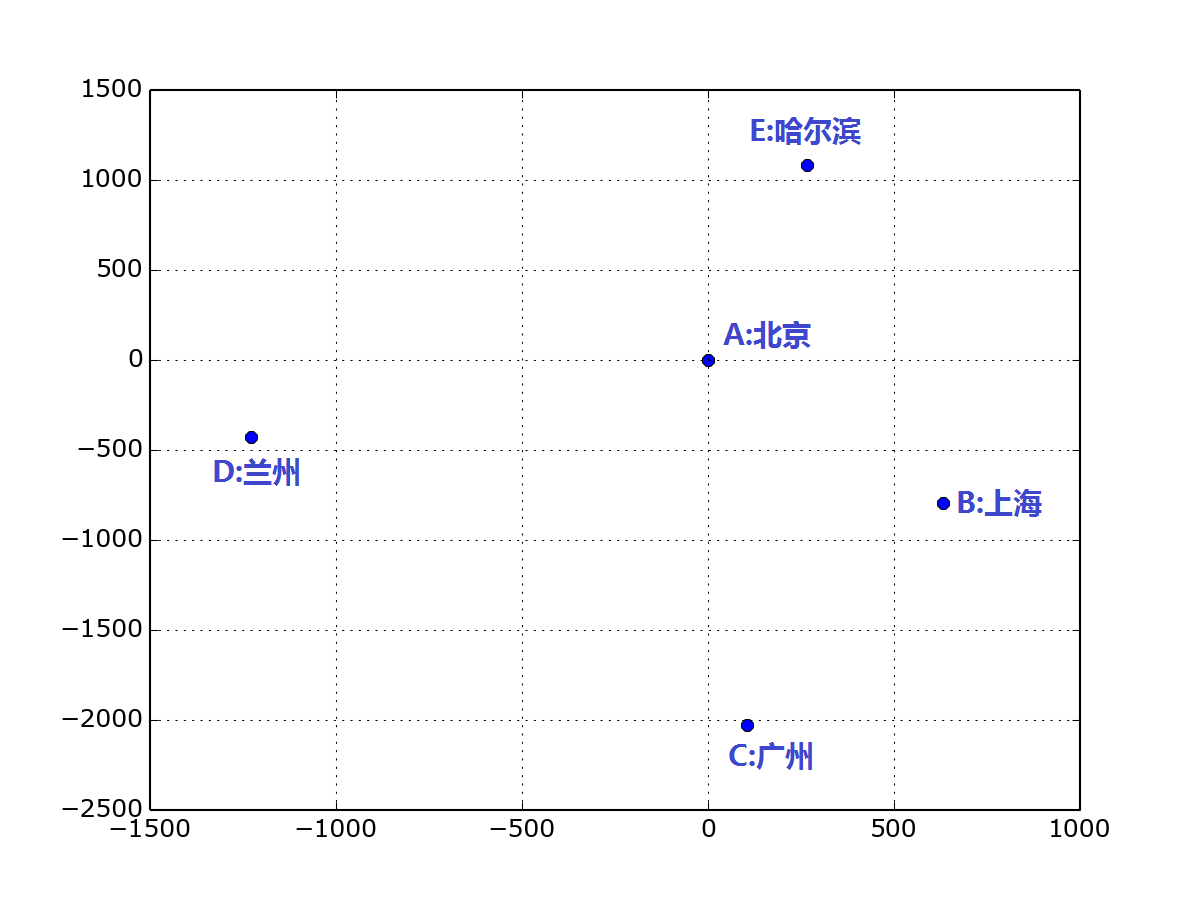
\includegraphics[width=0.48\textwidth]{trick/map_pure.eps}}}
\subfigure{\label{img:city distance}}\addtocounter{subfigure}{-2}
\subfigure{\subfigure[城市间两两距离]
			{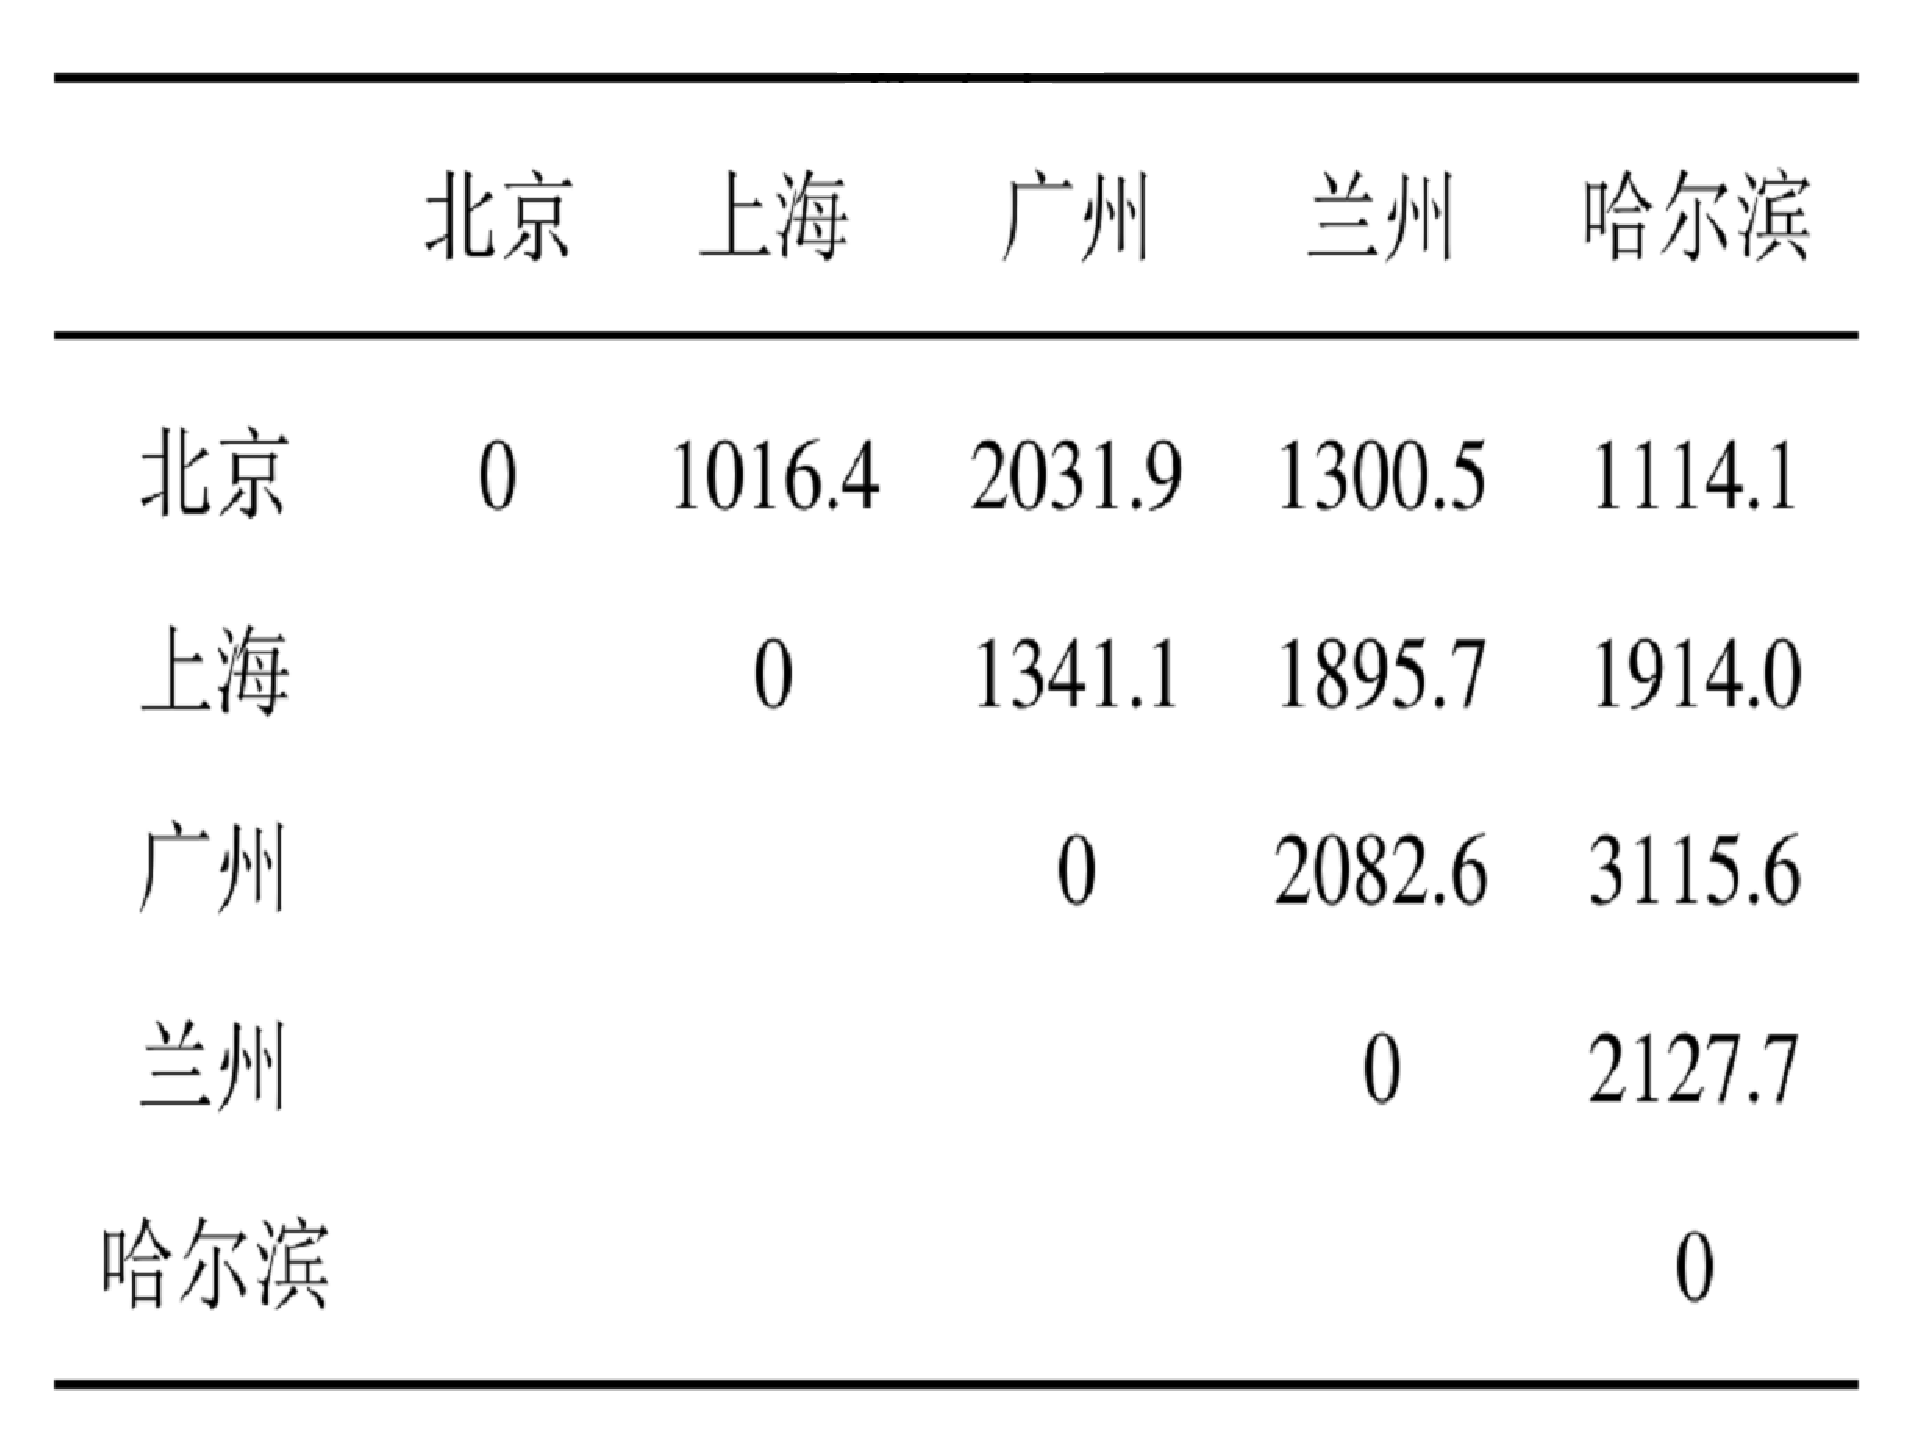
\includegraphics[width=0.45\textwidth]{trick/map_dist.eps}}}
\caption{五个城市的信息}
\vspace{-1em}
\end{figure}

如果现在我们不再知道各个城市的具体坐标,我们只知道图\ref{img:city distance}中两两城市之间的距离,那么如何通过图\ref{img:city distance}中的信息进行地图的重建,或者说根据距离推导出各个城市的坐标呢?这就是多维尺度分析所要完成的工作。

首先,我们假设这$n$个城市的坐标构成一个矩阵$X = [x_1, x_2, \cdots , x_n]^T$,那么城市$i$和城市$j$之间的欧式距离的平方为
\begin{equation}
s_{ij} = (x_i - x_j)^T (x_i, x_j)
\end{equation}
由$s_{ij}$可以构成一个$n\times n$的矩阵$S_{n\times n}$,这个矩阵我们称为距离矩阵,如果我们再定义Gram矩阵为
\begin{equation}
G_{n\times n} = HXX^TH
\end{equation}
其中,$H$为去中心化矩阵,定义为
\begin{equation}
H = I_n - ee^T
\end{equation}
其中,$I_n$为$n$阶单位矩阵,$e = \frac{1}{\sqrt{n}}(1, \cdots, 1)^T$,那么Gram矩阵可以推导为
\begin{equation}
G_{n\times n} = HXX^TH = \bigg[(x - \bar{x})^T (x - \bar{x})\bigg]
\label{equ:gram matrix}
\end{equation}
式中,$\bar{x}$为$X$的均值,通过式\eqref{equ:gram matrix},进一步可以推导得
\begin{equation}
G_{n\times n} = -\frac{1}{2}HSH
\end{equation}
由于欧几里得距离是正定的,因此Gram矩阵也是正定的,如果我们将Gram矩阵特征分解,则有
\begin{equation}
G_{n\times n} = P\Sigma P^T
\end{equation}
式中,$\Sigma$为Gram矩阵特征值构成的对角矩阵
\begin{equation}
\Sigma = \left[
\begin{array}{ccc}
\lambda_1 & &\\
&\ddots&\\
&&\lambda_n
\end{array}
\right]
\end{equation}
$P$为Gram的特征向量构成的矩阵,即$P = [p_1, \cdots, p_n]$。如果我们提取出Gram矩阵最大的k个特征值以及其对应的特征向量,那么通过
\begin{equation}
\hat{X} = \left[
\begin{array}{ccc}
\sqrt{\lambda_1} & &\\
&\ddots&\\
&&\sqrt{\lambda_k}
\end{array}
\right] 
[p_1, \cdots, p_k]
\end{equation}
我们将得到含有$n$个$k$维向量的矩阵$\hat{X}$,这个矩阵$\hat{X}$就是$X$在$k$维空间的一个映射。例如,在我们地图重构的问题中,通过图\ref{img:city distance}中的距离信息,当$k=2$时,我们求得
\begin{equation}
\hat{X} = \left[
\begin{array}{cc}
-45.6 & 434 \\
-677.1 & -362.1 \\
-149.3 & -1594.9 \\
1182.5 & 6.2 \\
-310.5 &1516.5
\end{array}
\right]
\end{equation}

如果将上述求得的坐标描绘在平面直角坐标系上,其结果如图\ref{img:map_mds_not_rot}所示。我们可以看到,这些点与真实分布十分相似,只相差一个水平镜像,我们将其镜像后的结果如图\ref{img:map_mds_rot}所示。镜像结果显示,重构的地图中,各个城市所在的相对位置与真实地图中城市的相对位置相同,但是不同的是,在重构的地图中,绝对位置改变了,例如我们可以看到,原来处于原点位置的北京现在不在处于原点。

\begin{figure}[htbp]
\centering
\subfigure{\label{img:map_mds_not_rot}}\addtocounter{subfigure}{-2}
\subfigure{\subfigure[重构后得到的直接结果]
			{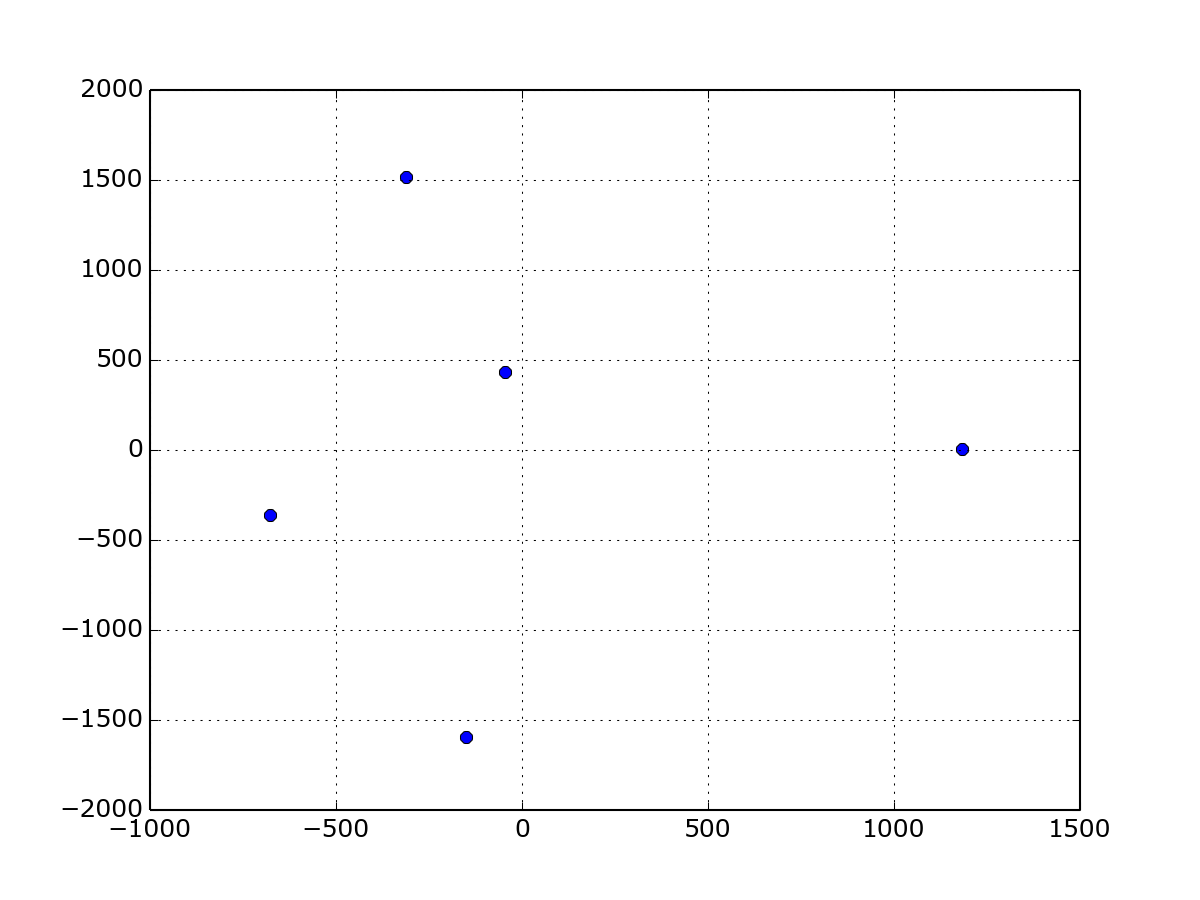
\includegraphics[width=0.45\textwidth]{trick/map_mds_not_rot.eps}}}
\subfigure{\label{img:map_mds_rot}}\addtocounter{subfigure}{-2}
\subfigure{\subfigure[镜像后的结果]
			{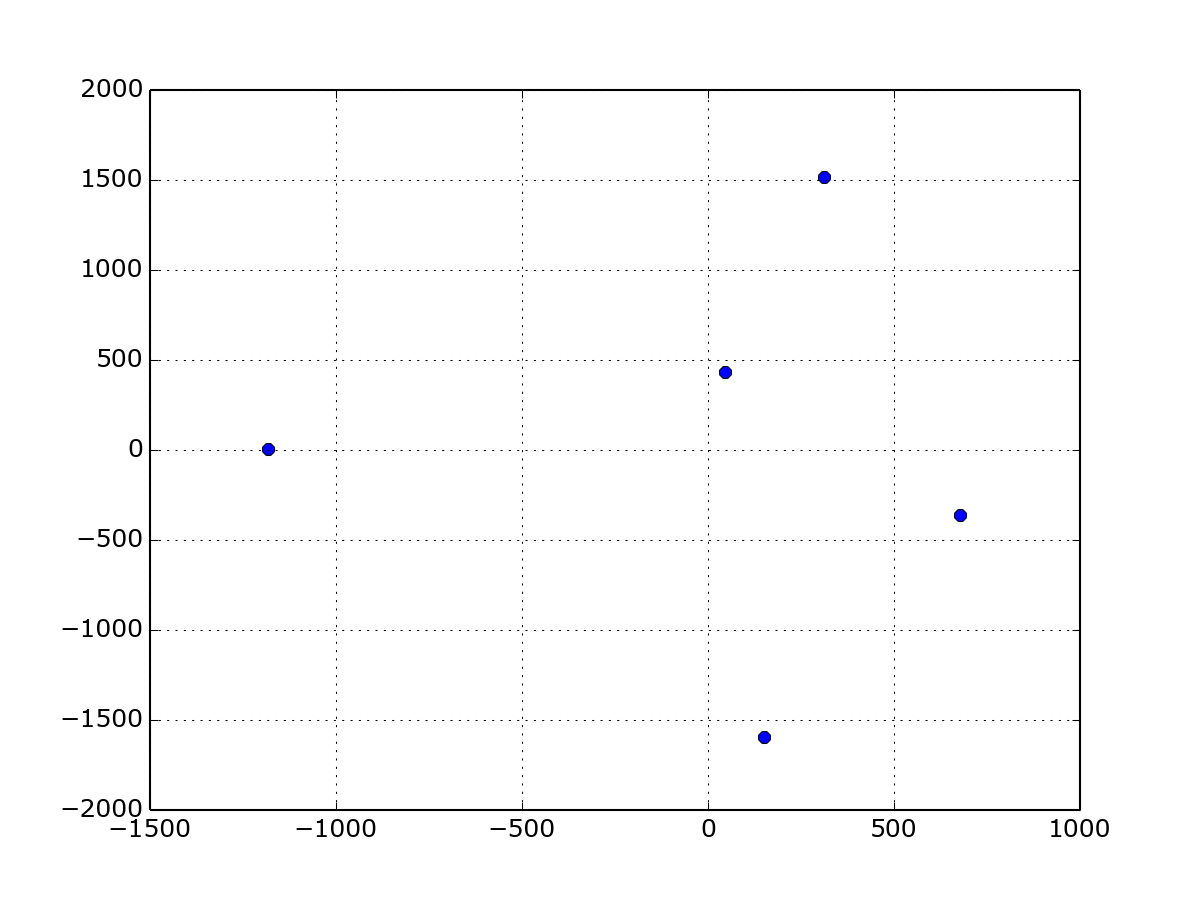
\includegraphics[width=0.45\textwidth]{trick/map_mds_rot.eps}}}
\caption{多维尺度分析对地图的重构}
\vspace{-1em}
\end{figure}

地图重构的例子并没有展现出多维尺度分析是如何降维的,因为这里只是从一个二维坐标转换到另一个二维坐标。但由于这个转换的过程中使用的欧几里得距离对于高维空间是可复用的,因此对于多维尺度分析的降维,我们先通过高维空间中的数据点两两求距离,得到平方距离矩阵,在通过这个平方距离矩阵求取Gram矩阵,将Gram矩阵特征分解,选取最大的$k$个特征值以及对应的特征向量,利用他们可以将原始的高维数据降到$k$维数据。例如,图\ref{img:MDS dim redu}描述了三维空间中的数据降到二维空间的过程。

\begin{figure}[htbp]
\centering
\subfigure{}\addtocounter{subfigure}{-2}
\subfigure{\subfigure[三维空间中的原始数据]
			{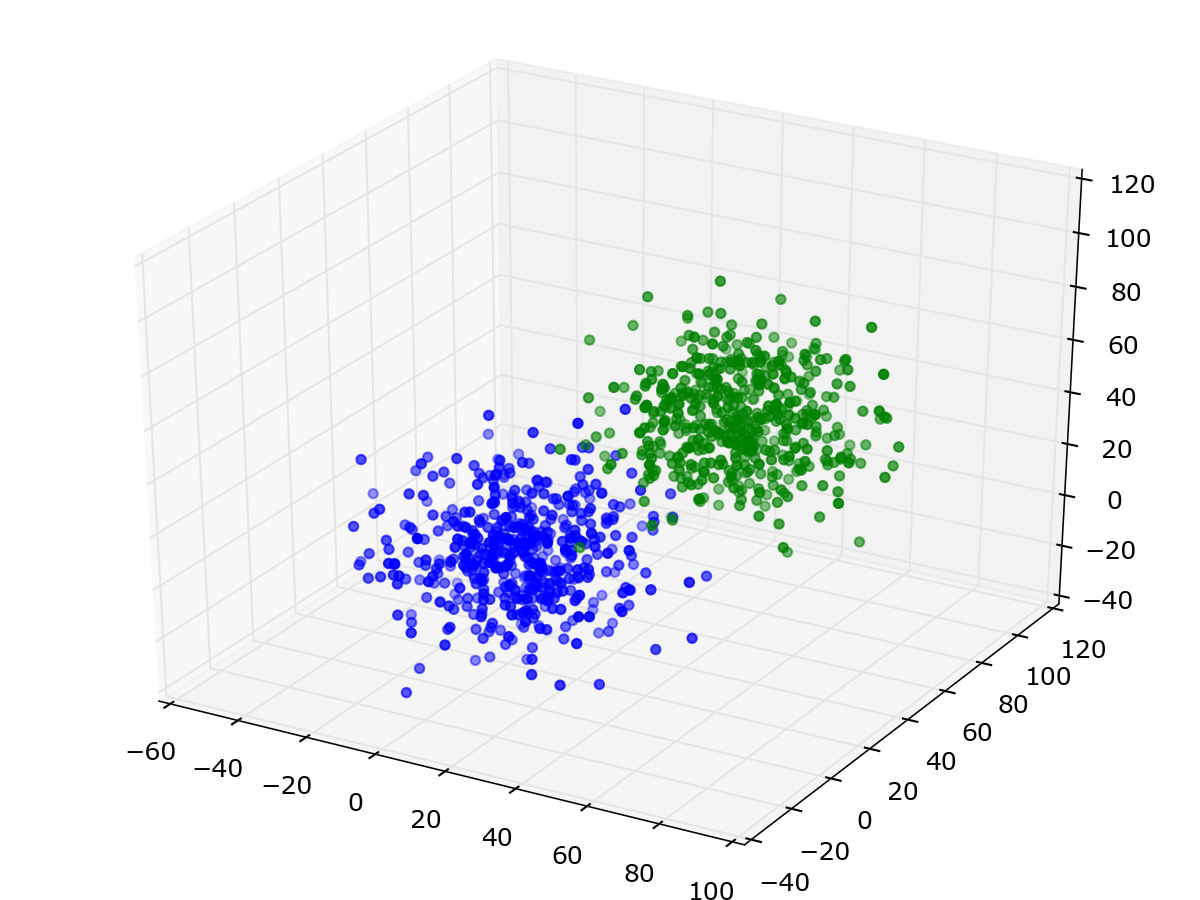
\includegraphics[width=0.45\textwidth]{trick/mds3D.eps}}}
\subfigure{}\addtocounter{subfigure}{-2}
\subfigure{\subfigure[降到二维空间后的数据]
			{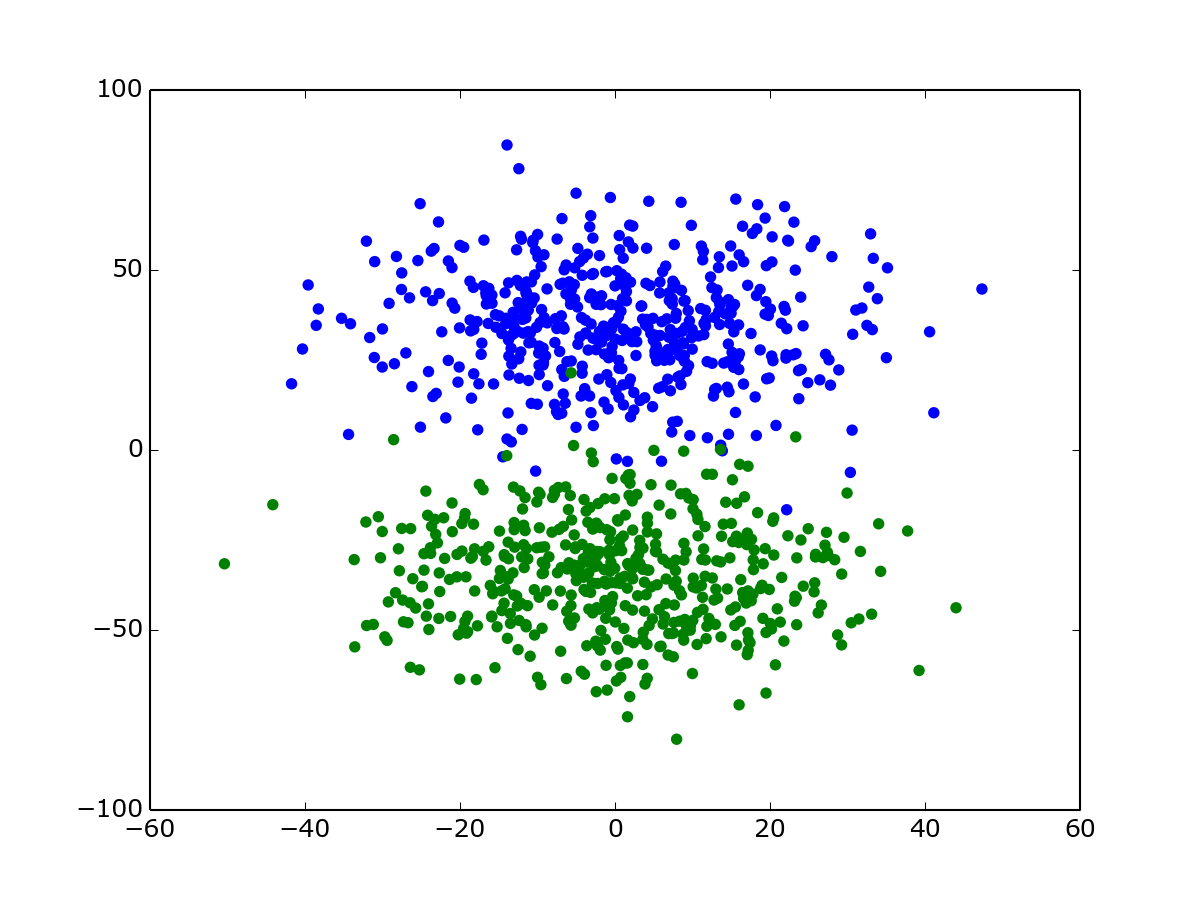
\includegraphics[width=0.45\textwidth]{trick/mds2D.eps}}}
\caption{多维尺度分析的降维}
\label{img:MDS dim redu}
\vspace{-1em}
\end{figure}

多维尺度分析并不是一个应用非常广泛的降维方法,其主要原因在于欧几里得距离,如图\ref{img:swiss roll 2}三维空间中AB两点,如果使用欧几里得距离(图中的绿线),那么我们认为这两点是十分接近的,因此降到二维空间后这两点将会靠得很近。但事实上AB两点相距很远,它们两者之间经过很长一段流形(图中的红线),而欧几里得距离忽视了这种距离。

\begin{figure}[!htbp]
\centering
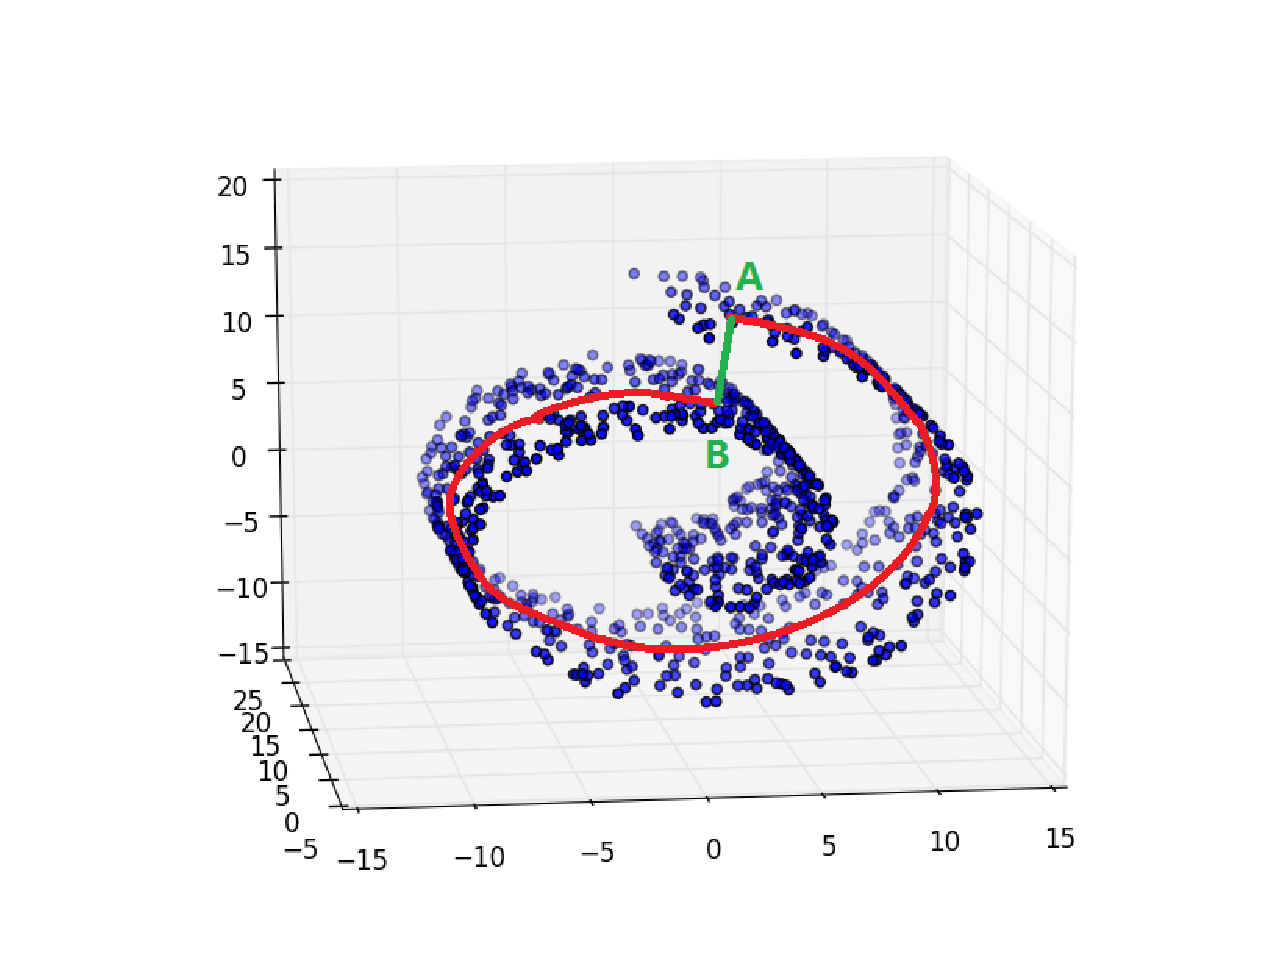
\includegraphics[width=0.8\textwidth]{trick/swissRoll2.eps}
\caption{Swiss Roll}
\label{img:swiss roll 2}
\end{figure}

尽管多维尺度分析并不常用,但是通过它可以引入流形学习中的一些经典算法,例如Isomap等,用以解决图\ref{img:swiss roll 2}中类似的情况,更多的讨论可参考文献xxxx

\BiSubsection{扩容}
x机器学习业内有一个共识,很多时候别人的分类性能比你的好并不意味着他的算法比你的好,更大的可能是他拥有比你更多的数据。数据是统计机器学习的命脉,没有数据,再好的模型也难以奏效。如果把机器学习中的算法比作是航天器的引擎,那么数据就是航天器的燃料。这种现象在深度学习中尤为明显,特别是卷积神经网络。深度学习需要大量的数据样本,这个需求量随着识别任务复杂性的增加而增加。尽管互联网的大数据时代数据容易获取,但有些时候数据是有限的,对于有限的数据集,我们可以通过一定的手段将数据集的容量扩大。例如在字符识别任务中,我们知道,字符微量的扭曲、旋转、放大、缩小对人而言是不会影响字符的识别,因此,我们可以对原始数据进行随机地选取上述一个或多个变换,使得数据的容量增大。又例如,真实生活中的图片,水平镜像、对比度微调、饱和度微调等操作对人而言不影响最终的图像识别,我们利用这个特性对图像采取一定的变换便可很大程度地增大训练集的容量,例如,仅仅是图像的水平镜像就可以使得数据集扩大一倍。

数据的扩容,实质上是一种贝叶斯先验,因为我们对数据采取的变换策略不会影响最终的分类,例如,我们不会对字符进行镜像处理。这种先验,使得模型可以免疫一定的干扰,例如采取了水平位移变换策略的数据集受到水平位移的影响就减小了,这就提高了模型的泛化能力。

\BiSection{训练技巧}
x网络的训练过程中,我们会使用到一些技巧,这些技巧大部分的目的都在于抑制网络的过拟合以及防止准则函数陷入局部最优解。由于这些技巧众多,我们无法在这里涵盖所有,因此我们只挑选了几个常用且重要的技巧,分别是学习率的设定、动量项的使用以及权衰减。
\BiSubsection{学习率}
x在梯度下降算法中,每次求得准则函数相对于参数的梯度$\partial J /\partial \theta$后,我们并不是直接以这个值作为参数的增量,工程中,我们还应对梯度乘上一个学习率$\eta$,即参数更新的公式为
\begin{equation}
\theta = \theta - \eta \frac{\partial J}{\partial \theta}
\label{equ:grandianDes}
\end{equation}
学习率的作用类似于下山时步伐的长度,步伐过长,则有可能导致准则函数震荡,影响收敛速度,如果步伐十分大,则会导致发散现象,哪怕准则函数是凸函数,存在唯一极值点,过大的学习率也会使其发散。例如,假设准则函数设定为二次函数,即
\begin{equation}
J(\theta) = \theta^2
\end{equation}
显然这是一个凸函数,存在唯一极值点,即$\theta = 0$处。如果我们对这个准则函数求偏导,则为
\begin{equation}
\frac{\partial J}{\partial \theta} = 2\theta
\end{equation}
即准则函数$J(\theta)$上的每一点$\theta$,其梯度都等于$2\theta$。假设现在$\theta = 2$,那么我们可以很容易计算得到其梯度为$4$,此时,最优的学习率为$\eta ^* = 0.5$,因为$2-0.5\times 4$恰好使得$\theta$落入到最优解即$\theta = 0$处,如图\ref{img:eta=0.5}所示。如果我们的学习率选取得比最优学习率大,假设我们选取为$\eta  = 0.7$,那么参数$\theta$就会沿着$2\rightarrow \rightarrow -0.8\rightarrow 0.32 \rightarrow -0.128 \cdots$的轨迹下降,如图\ref{img:eta=0.7}所示。倘若我们的学习率再大一些,为两倍的$\eta$时,即当$\eta  = 1$时,$\theta$就会在$+2$和$-2$两者之间变换而不会进入别的位置,如图\ref{img:eta=1}所示。当学习率大于两倍的最优学习率,例如$\eta = 1.5$,那么$\theta$就会沿着$2\rightarrow -4 \rightarrow 8\rightarrow -16$的轨迹移动,此时准则函数便发散,这个过程如图\ref{img:eta=1.5}所示。

\begin{figure}[htbp]
\centering
\subfigure{\label{img:eta=0.5}}\addtocounter{subfigure}{-2}
\subfigure{\subfigure[$\eta = 0.5$]
			{\includegraphics[width=0.4\textwidth]{trick/eta05.eps}}}
\subfigure{\label{img:eta=0.7}}\addtocounter{subfigure}{-2}
\subfigure{\subfigure[$\eta  = 0.7$]
			{\includegraphics[width=0.4\textwidth]{trick/eta075.eps}}}
\subfigure{\label{img:eta=1}}\addtocounter{subfigure}{-2}
\subfigure{\subfigure[$\eta  = 1$]
			{\includegraphics[width=0.4\textwidth]{trick/eta1.eps}}}
\subfigure{\label{img:eta=1.5}}\addtocounter{subfigure}{-2}
\subfigure{\subfigure[$\eta = 1.5$]
			{\includegraphics[width=0.4\textwidth]{trick/eta15.eps}}}
\caption{不同的学习率对收敛的影响}
\vspace{-1em}
\end{figure}


但是较大的学习率并不意味着一无是处,学习率稍微大一些,可以加快收敛速度,而且可以越过一些局部极小值(但是对于高尔夫球场形状的局部极小值无能为力)。在工程中,学习率的选取我们的建议是,先将学习率初始化为一个较大的数值,如果准则函数发散了,那么我们就将其缩小2倍,直到准侧函数能开始下降为止。另外一种做法是,先初步计算梯度的数值大小,将学习率设定为一个比梯度小3个数量级的常数,例如,我们上面的计算得到的梯度是4,那么学习率可以设定为0.001。

事实上学习率固定为一个常数并不是一个较好的策略,因为初始时设定的学习率相对于训练的后期而言是过大的,这将会导致准则函数在极小值附近震荡。一种解决方法是将学习率也设定为一个学习参数,这个参数随着网络的训练而不断地更新,另外一种虽然愚蠢但行之有效的方法是,不断地关注准则函数的下降情况,一旦感觉下降开始出现震荡或平谷现象就将学习率调小1个数量级。

\BiSubsection{动量项}
x很多时候,在参数校正的过程中,仅仅使用学习率是不行的,一般还应使用动量项。动量项,即在参数的更新过程中,引入一个动量因子,更新规则描述为
\begin{equation}
\theta_{t+1} = \theta_t - \eta(1-p)\frac{\partial J(\theta)}{ \partial \theta_t} - p * (\theta_{t-1} - \theta_{t-2})
\label{equ:momentum1}
\end{equation}
式中,$t$代表第$t$次参数更新,$\eta$为学习率,$p$为动量项因子,这个因子一般选取为$p = 0.9$。式\eqref{equ:momentum1}实际上讲述了这样一件事:参数更新的时候,增量不仅仅依赖于当前的梯度,还依赖于上一次权值变化量的$p$倍,因此参数的更新,带着类似于物理中动量的项,即$p * (\theta_{t-1} - \theta_{t-2})$,它也被称之为动量项。动量项可以使得准则函数快速地下降,并且可以越过一些较为平坦的局部极值。如果读者有数字信号处理的背景,式\eqref{equ:momentum1}实际上是一个脉冲响应低通滤波器,目的在于平滑参数的更新过程\citeup{Duda}。

但由于\eqref{equ:momentum1}需要记录上一次的参数增量,这在实际编码中需要一定的内存,而且实现起来也不方便,另外一种关于动量项的简单用法是
\begin{equation}
\theta_{t+1} = p\theta_t - \eta\frac{\partial J(\theta)}{ \partial \theta_t}
\end{equation}
式中,$p$为动量项系数,一般取0.9。动量项的使用,确实可以在一定程度上避免局部最优解,例如,假设准则函数为
\begin{equation}
J(\theta) = -5\theta^3 - 80\theta^2 - 400\theta - 700
\end{equation}
我们可以很容易地计算准则函数在任意一点的梯度为
\begin{equation}
\frac{\partial J(\theta)}{ \partial \theta} = -15\theta^2 - 160\theta - 400
\end{equation}
假设学习率设置为常数0.001,如果不采用动量项,即参数更新的规律为
\begin{equation}
\theta =\theta - 0.001\frac{\partial J(\theta)}{ \partial \theta} 
\end{equation}
那么准则函数的收敛过程如图\ref{img:no momentum}所示,我们可以看到,在收敛的后半阶段,参数$\theta$会收敛到局部极值,但如果我们使用一个系数为0.9的动量项,即参数更新规则为
\begin{equation}
\theta =0.9 * \theta - 0.001\frac{\partial J(\theta)}{ \partial \theta} 
\end{equation}
此时的准则函数收敛过程如图\ref{img:has momentum}所示,我们可以看到,动量项的引入,使得参数$\theta$在平坦的局部极值区域内依然带有冲劲,这个性质使得它可以跨越一些较小的局部极值而不至于陷入其中。
\begin{figure}[htbp]
\centering
\subfigure{\label{img:no momentum}}\addtocounter{subfigure}{-2}
\subfigure{\subfigure[不使用动量项]
			{\includegraphics[width=0.45\textwidth]{trick/noMonent.eps}}}
\subfigure{\label{img:has momentum}}\addtocounter{subfigure}{-2}
\subfigure{\subfigure[使用系数为0.9的动量项]
			{\includegraphics[width=0.45\textwidth]{trick/hasMonent.eps}}}
\caption{动量项对收敛的影响}
\vspace{-1em}
\end{figure}

\BiSubsection{权衰减}
所谓权衰减,即在权值更新完毕后对所有的权值乘以一个小于1的常数$e$,$e$一般取0.999左右。之所以要这样做的原因,是因为我们希望权值保持在较小的范围内,因为更小的权值使得净激活停留在激活函数的非饱和区域内。使用权衰减的参数更新规则为
\begin{equation}
\theta = e*\theta
\label{equ:weight decay}
\end{equation}
关于权衰减的另一种解释是,在准则函数中,我们加入一个二范数惩罚,即新的准则函数定义为
\begin{equation}
J_{new}(\theta) = J(\theta) + \frac{\lambda}{2} \theta^T\theta
\label{euq:penalyL2}
\end{equation}
\eqref{euq:penalyL2}中的第二项也被称为正则项。如果我们对式\eqref{euq:penalyL2}求导,则为
\begin{equation}
\frac{\partial J_{new}(\theta)}{ \partial \theta} = \frac{\partial J(\theta)}{ \partial \theta} + \lambda \theta
\end{equation}
因此权值的更新规则为
\begin{equation}
\theta = \theta - \frac{\partial J_{new}(\theta)}{ \partial \theta} = \bigg(\theta -  \frac{\partial J(\theta)}{ \partial \theta}\bigg) - \lambda \theta
\end{equation}

这事实上等价于是式\ref{equ:weight decay},即在权值更新后乘上一个衰减系数。我们之所以使用权衰减,或者说加入二范数正则(这两个命题等价),实际上它代表着一种贝叶斯先验,即我们对于权值的期待(希望它是较小的值)。

需要注意的是,在神经网络中,我们一般只针对权值进行权衰减,而不针对偏置进行权衰减,因为我们希望获得较大的偏置。至于为什么,这实际上并没有为什么。


\BiSection{编码技巧}
x尽管我们讨论了大量的理论内容,这些理论内容具体实现在代码上并不是一件简单的事。代码如何设计以及如何测试是我们遇到的最大问题。与传统的软件工程所不同的是,机器学习中的测试无法使用单元测试,因为在单元测试中我们需要知道代码的期望输出,机器学习自学习的特点注定了我们无法知道其正确输出是什么。代码的测试,更多时候是凭感觉,尽管如此,我们还是有办法进行一些简单测试的,在本小节中,我们将会介绍面向对象的设计思路以及用于测试的梯度校验。
\BiSubsection{面向对象技术}
x神经网络的设计中,不同层可以采用不同的激活函数,也可以采用不同的网络结构,例如卷积层或全连接层。这些不同层之间都有两个共同的特性。在前向传播过程中,无论是什么形式的层都接收前一层传播的激活,而在反向传播过程中,所有的层都接收后一层传播回来的误差,并利用该层的输入与输出对参数进行校正。尽管不同结构的网络层其校正方式不同,但这个过程可以使用面向对象的技术实现。为了方便讨论,我们将用JAVA的语法来描述这个过程\footnote{然而JAVA并不是一门适合数值运算的语言}。我们定义一个接口Layer,它含有两个方法,即fprop和bprop,分别对应着前向传播和反向传播。fprop接收一个参数,即前向传播得到的输入数据,bprop接收三个参数,分别是反向传播回来的误差、该层的输入以及该层的输出,事实上,bprop也可以设定为只接收一个参数,即反向传播回来的误差,而该层的输入以及该层的输出设定为成员变量。具体的网络结构,例如ConvlutionLayer、FullConnectLayer等实现这个接口,并实现这个接口中的两个方法,利用多态性,就可以容易地实现不同层执行不同的更新方法。如果网络的所有层都采用同一个激活函数,那么这个激活函数可以直接写到接口中(尽管JAVA要JDK9中才能在接口中提供方法的实现,但我们可以利用继承让具体的层继承另一个类)。如果网络的所有层采用的是不同的激活函数,那么我们可以通过策略模式将激活函数抽象成一个接口,具体的激活函数实现这个接口,在具体网络层实现类的构造方法中通过依赖注入将具体的激活函数实现注入到网络层的类中,利用多态性,可以让不同的层执行不同的激活函数,而这些不同的激活函数又可以实现代码复用。最后将这些不同的网络层组合到一个神经网络实现类中,例如CNN或DBN,即可完成整个网络的编码工作,整个工程代码的UML图如图\ref{img:UML}所示。
\begin{figure}[!htbp]
\centering
\includegraphics[width=1\textwidth]{trick/UML.eps}
\caption{神经网络类图设计}
\label{img:UML}
\end{figure}
\BiSubsection{梯度校验}
x在神经网络的编码中,一个令人头疼的问题是反向传播是否已经被正确编码。很多时候,错误的编码并不会导致严重的错误,但它会影响最终的分类效果。在debug过程中,一个十分有效的用来检测编码是否正确的方法是梯度校验。假设我们要优化以$\theta$为参数的准则函数,在梯度下降中,我们的更新规则如式\eqref{equ:grandianDes}所示。假设我们通过算法计算得到准则函数相对于参数的梯度,例如,在全连接神经网路中,这个梯度一般为
\begin{equation}
\frac{\partial J(\theta)}{\partial \theta} = \delta \cdot \frac{\partial f(net)}{\partial net} \frac{\partial net}{\theta}
\label{eqe:trickxxxx}
\end{equation}
式\eqref{eqe:trickxxxx}本质上是利用导数公式取计算梯度,正如我们要算$J(\theta) = \theta ^2$的导数,那么我们可以通过其导数即$J'= 2 \theta$直接计算在某点处的导数,但我们还可以通过另一种方式计算导数。回想高等数学中关于导数最原始的定义,导数即增量的极限,定义为
\begin{equation}
\frac{\partial J(\theta)}{\partial \theta} = \lim\limits_{\Delta\theta \rightarrow 0} \frac{J(\theta + \Delta\theta) - J(\theta)}{\Delta\theta}
\label{equ:limit}
\end{equation}
也就是说,如果我们给某个参数$\theta_i$加上一个非常小的增量$\Delta\theta$,假设为0.001,那么利用式\eqref{equ:limit}的原理,我们对比$\theta_i$没有加上这个增量之前准则$J(\theta)$的值与加上增量之后准则的值,这两个值作差,再除以增量,将会得到准则函数相对于$\theta_i$这个变量的梯度。这种方法求得的梯度$\Delta^*_\theta J(\theta)$与利用式\eqref{eqe:trickxxxx}$\Delta_\theta J(\theta)$满足如下关系
\begin{equation}
\Delta^*_\theta J(\theta) \approx \Delta_\theta J(\theta)
\end{equation}

如果$\Delta\theta$取得足够小,那么这两者近似程度非常高,但是实际编码中$\Delta\theta$不应取得过小,因为计算机的浮点运算会带来误差,一般而言,$\Delta\theta$取0.001左右就足以用来验证梯度了。另外需要注意的是,这种近似性只会在较深的层中发生,在较浅的层中误差会较大,因为反向传播是贪婪的,所以随着误差越传越远,梯度的偏离也会越大。利用梯度校验在可以方便检验代码正确性的同时,还可以在梯度校验的过程总发现,如果激活函数是Sigmoid函数,而网络有是深度网络,那么不经过预训练的网络会出现梯度消失现象。

\BiSection{本章小结}
x本章中我们讨论了神经网络训练过程中一些会使用到的技巧,我们只介绍了一些通用的技巧,更多的特殊技巧如dropout、maxout等我们并没有讨论,更多的讨论可参考文献\cite{baldi2013understanding}和\cite{goodfellow2013maxout}。本章介绍的技巧中,降维自身就是一个很大的话题,并不仅仅作为技巧而存在,它是机器学习的一个分支,我们只介绍了两种降维方式,更多的降维方法如Isomap、局部线性嵌入、基于核的主成分分析等可参考文献\cite{tenenbaum2000global,roweis2000nonlinear,scholkopf1998kernel}。最后还需要说明一点,网络的设计者不应迷信这些技巧,它们只是起到指导作用,具体是否可行要具体任务具体分析。


\BiChapter{GPU计算}{performance}

上世纪六十年代提出的摩尔定律到目前为止已经持续了半个多世纪,硅技术似乎已经难以再有重大突破,摩尔定律在未来几年或将成为过去。然而当前计算机的计算能力仍不足以满足人们的需求,并行技术的发展在一定程度上缓解了这种压力,某种程度上而言,计算并行化可以看做是摩尔定律的一种延伸。

GPU(Graphic Processing Unit)又称“图形处理器”,是相对于CPU的一个概念,其最初目的是满足计算机图形界面中人们对于实时、高清的三维图形的需求。在图形开发中,由于图形渲染及变换等操作是带有可并行特征的,因此对于GPU的设计者而言,他们更倾向于添加更多的核心而不是提高核心的运行效率,通过多个核心以及线程技术,使得同一条指令可在每个元素上执行。此外,他们还取消了CPU中的缓存与逻辑控制部件,因此GPU适用于计算密集的并行计算,而CPU更适用于含有复杂流控的计算。

但是最初的GPU是为图形开发者而开发的平台,对于非图形开发者而言,使用GPU进行通用计算并不是一件容易的事。为此,ATI公司(已被AMD收购)于2005年提出的ATI Stream方案,NVIDIA公司在2007年推出的CUDA平台,都是为了解决GPU通用计算问题而做出的努力。在GPU通用计算不断发展的同时,新的规范也被不断地提出,Apple公司在2008年提出OpenCL(Open Computing Language)规范,微软提出的DirectCopmute规范,其目的都在于制定了一套API,并在此基础上开发GPU通用计算软件。

在这些GPGPU(General Purpose GPU)方案中,由于CUDA为开发者提供了一个类似于C的编程环境,使用者可以快速学习,所以受到了广泛的使用。


\BiSection{GPU体系结构}
x相比于CPU而言,GPU由于其设计原则就是针对密集运算的,所以在浮点运算上占着先天优势。近几年CPU在运算效率上的提升缓慢,与此同时,GPU计算却飞速发展,其运算性能已远远超过CPU。如图所示是Intel的CPU与NVIDIA的GPU在各个型号上每秒浮点运算量的对比。相比于CPU而言,GPU由于其设计原则就是针对密集运算的,所以在浮点运算上占着先天优势。近几年CPU在运算效率上的提升缓慢,与此同时,GPU计算却飞速发展,其运算性能已远远超过CPU。如图\ref{img:GPUvsCPU}所示是Intel的CPU与NVIDIA的GPU在各个型号上每秒浮点运算量的对比\footnote{图片出自于NVIDIA的官方技术文档《CUDA C Programming Guide》}。

\begin{figure}[!htbp]
\centering
\includegraphics[width=0.57\textwidth]{GPU/GPUvsCPU.eps}
\caption{GPU与CPU在每秒浮点运算量上的差异}
\label{img:GPUvsCPU}
\end{figure}

由于GPU中取消了逻辑控制单元,相比于CPU其体系结构有着很大的不同。典型的CPU结构带有三级缓存,数据由内存经过三层缓存后才进入到处理器核心,这个结构如图所示。GPU同样带有缓存,这个缓存一般只有两级,与CPU不同的是,CPU中只有一个处理器,而GPU中并没有处理器核心的概念,取而代之的是流处理器簇(Streaming Muntiprocessor),在一个GPU中往往含有多个流处理器簇,尽管它们与CPU处理器核心有着很大的差异,但某种程度上也可以看做是GPU的核心,整个GPU的结构如图所示。

\begin{figure}[htbp]
\centering
\subfigure{\label{img:CPU}}\addtocounter{subfigure}{-2}
\subfigure{\subfigure[CPU结构]
			{\includegraphics[width=0.32\textwidth]{GPU/CPU.eps}}}
\subfigure{\label{img:GPU}}\addtocounter{subfigure}{-2}
\subfigure{\subfigure[GPU结构]
			{\includegraphics[width=0.46\textwidth]{GPU/GPU.eps}}}
\caption{CPU与GPU结构差异}
\vspace{-1em}
\end{figure}

CPU为了实现多核技术,往往在一个芯片中集成多个CPU核心,例如在Intel i7处理器中含有4个CPU核心,多核心使得CPU可以并行执行计算,但相比于GPU而言,CPU的并行粒度是非常大的。例如要将一个含有100个元素的向量的每一个元素乘上一个常数2,那么对于4核的CPU,我们可以指派1号CPU执行第1$\sim$25个元素的操作,2号CPU执行第26$\sim$50个元素的操作,但对于GPU而言,它可以直接开辟100个线程,每个线程针对每个元素进行操作,这些线程是并行线程而不是并发线程,因此GPU可以实现小粒度的并行。

GPU只所以能开辟大规模线程是因为一个GPU包含了一个流处理器簇阵列,这个阵列由多个流处理器簇构成,例如费米架构的GPU的阵列大小为16。而每个流处理器簇又包含了几十个到几百个的CUDA核心,例如,采用开普勒架构的GPU每个流处理器簇包含48个CUDA核心,而采用费米架构的GPU每个流处理器簇包含192个CUDA核心。这些核心并不类似于CPU的核心,CPU的每个核心只能执行一个线程,而CUDA核心可以并行执行多个线程。

GPU的线程由线程网格管理,线程网格可以看做是一个二维网格,这个结构如图\ref{img:thread grid}所示。在这个网格中,一个维度是线程块,另一个是线程束。每个GPU核心最多可包含65536个线程块,每个线程块最多可包含512个线程束,这意味着我们可以一次开辟最多大约3300万个线程,目前的费米架构已经实现每个线程块可包含1024个线程束,因此它最多可开辟6600万个线程。但这只是说我们可以在代码中开辟线程,并不意味着执行线程也是这个数量级。事实上,每个流处理器簇可执行的线程数量是有限制的,这个数量级大约是一千左右。

\begin{figure}[!htbp]
\centering
\includegraphics[width=0.6\textwidth]{GPU/threadGrid.eps}
\caption{线程网格}
\label{img:thread grid}
\end{figure}

实际中在跑的线程数大约为几万,然而我们却可以在代码中开辟几千万的线程,这得益于GPU对硬件的隐藏机制,类似于操作系统的虚拟地址,GPU会自动地将这几千万的虚拟线程在几万实际线程中调度,而程序员不需要参与到这个过程中,只需要在代码中开辟线程即可。这个机制使得硬件升级扩展变得简单,因为虚拟的线程与实际调度的线程是分离的,GPU为我们自动调度,我们可以随意的更换未来更多核心的GPU而不需要改动我们的代码。

为了更好地理解线程块与线程的概念,我们举一个GPU中实现两个向量相加的例子,如代码8.1所示

\begin{lstlisting}[language=C, numbers=left, frame=shadowbox, rulesepcolor=\color{cadegrey}, caption=\text{向量加法内核函数}]
__global__ void add(int *c, int *a, int *b){
	int tid = blockId.x;
	c[tid] = a[tid] + b[tid];
}
\end{lstlisting}

代码8.1中的的\_\_ kernel\_ \_ 代表这是一个在GPU中执行的代码,我们称其为内核函数。由\_\_ kernel\_\_ 标记的代码将由nvcc编译器编译,而没有这个标记的函数将由C++的编译器编译\footnote{例如Windows操作系统下的msvc或Linux操作系统下的gcc}。第2行代表获取当前的线程号,这里我们假定线程号就是线程块的编号,即默认每个线程块只有一个线程在运行。如果每个线程块有多个个线程在执行,那么第2行代码应改为

\begin{lstlisting}[language=C, frame=shadowbox, rulesepcolor=\color{cadegrey}]
int tid = threadIdx.x + blockId.x + blockDim.x;
\end{lstlisting}

观察图\ref{img:thread grid},这实质上类似于二维索引空间转换为线性空间的代码。代码8.1中的第3行代表每个线程执行一个操作,即将向量a中的第tid个元素与向量b中的第tid个元素相加,并存储在向量c的第tid个元素中。这可以理解为,代码8.1会做为一个副本分发给各个线程,各个线程拿到这段代码后,根据自己的线程ID(即tid)执行向量a和向量b中的第tid的元素的操作。


\BiSection{CUDA}
xCUDA(Compute Unified Device Architecture)是NVIDIA公司在2007年推出的高性能运算平台,它可以让GPU在执行常规的图形渲染的基础上额外地实现高性能的通用并行计算。CUDA包含了CUDA指令集架构以及GPU内部的并行计算引擎,通过利用 GPU 的处理能力,可大幅提升计算性能。支持CUDA平台的GPU包括NVIDIA Tesla 、NVIDIA Quadro 以及NVIDIA GeForce多个系列,其价格也涵盖了高端到底端多个市场,使得CUDA能够满足从消费级到专业级等多个方面的需求。目前为止, CUDA已经应用到图像与视频处理、计算生物学、流体力学模拟、金融风险分析、地震分析等多个领域,全球五百强企业以安装700多个基于CUDA的GPU集群,这些公司包括了能源领域的斯伦贝谢与雪佛龙以及银行业的法国巴黎银行等。

在CUDA中,程序员需要手工将数据从内存中迁移到GPU中,还需要负责GPU内存的回收,例如,为了执行两个向量的加法,其片段如代码8.2所示

\begin{lstlisting}[language=C, numbers=left, frame=shadowbox, rulesepcolor=\color{cadegrey}, caption=\text{GPU中向量加法的调用过程}]
int a[N], b[N], c[N];
int *dev_a, *dev_b, *dev_c;
//init a[N], b[N].....
cudaMalloc((void**)&dev_a, N*sizeof(int));
cudaMalloc((void**)&dev_b, N*sizeof(int));
cudaMalloc((void**)&dev_c, N*sizeof(int));
cudaMemcpy(dev_a, a, N*sizeof(int),cudaMemcpyHostToDevice);
cudaMemcpy(dev_b, b, N*sizeof(int),cudaMemcpyHostToDevice);
add<<<N, 1>>>(dev_c, dev_a, dev_a);	
cudaMemcpy(c, dev_c, N*sizeof(int),cudaMemcpyDeviceToHost);
cudaFree(dev_a);
cudaFree(dev_b);
cudaFree(dev_c);
\end{lstlisting}

在代码8.2中,我们先在GPU中申请内存,即对应的4$\sim$6行,随后在7$\sim$8行中将内存中的数据迁移到之前申请的GPU内存中。第9行执行代码8.1实现的加法内核函数,在GPU中开辟N个线程块,每个线程块含有1个线程,GPU完成计算后,我们在第10行将计算结果从GPU中迁移回内存,最后第11$\sim$13行释放之前申请的内存。释放内存是重要的,如果申请了内存不释放便会导致内存泄露,当内存消耗完毕后程序崩溃。

我们不由感叹,为了执行一个简单的向量加法就要编写如此多的代码,我们需要手工申请内存,手工将数据迁移到GPU中,手工调用内核函数,调用完毕后需要手工将计算结果从GPU中迁移回来,最后还需要手工释放申请的内存。如果用户不是专业的程序员,那么代码编写的过程十分困难。因此,在CUDA之上有多个团队为机器学习研究人员开发了专门的第三方库,我们将会介绍几个常见的包。
\BiSection{Cudamat}
xCudamat是一个由多伦多大学开发的一套针对于Python的开源第三方库\citeup{cudamat},它基于CUDA,在实现GPU高性能计算的同时保留了Python“语法优雅”的特性,所以使用者可以很方便地在Python语法层次上调用矩阵运算库。开发Cudamat的目的是为了方便机器学习建模,使科研人员从繁琐的CUDA编程中解放出来,由于GPU在浮点并行运算上巨大的优势,所以在计算密集的矩阵运算任务中Cudamat相对于numpy或MATLAB,其运算速度大约提升了50倍左右。

在Cudamat中,开发者已为我们重载了一些运算符,这使得矩阵的四则运算运算以及面向元素的四则运算,以及矩阵的切片、转置等操作不再需要编写大量的代码或调用对应的函数。此外,开发者还提供了一些常用的函数,例如面向元素的exp()、log()、sqrt()、pow(),矩阵的乘法以及面向轴的求和、随机矩阵的生成等。例如,为了实现一个logistic函数,只需要在Python中只书写代码8.3中的语句

\begin{lstlisting}[language=Python, frame=shadowbox, rulesepcolor=\color{cadegrey}, caption=\text{Cudamat中logistic的实现}]
def logistic(A):
   expTerm = cudamat.CUDAMatrix(numpy.random.randn(A.shape))
   cm.exp(-A, target=expTerm)
   return 1 / (1 + expTerm)
\end{lstlisting}

尽管Cudamat并没有将CUDA的所有功能都囊括其中,但在机器学习中常用的功能基本都实现了,所有我们可以在不需要了解底层CUDA的前提下高效地建立数学模型的代码,减轻了我们的工作量。


\BiSection{Gnumpy}
x在Python科学计算中,numpy与scipy两个第三方包充当着重要角色,其中numpy凭借其优美的语法实现以及高效地执行速率深受人们喜爱。在numpy中,有着许多巧妙的设计,比如广播特性、切片、方便的元素存取、丰富的函数等。其语法特性与MATLAB接近,几乎MATLAB上能实现的功能在numpy中都能找到对应的实现,此外还加入一些MATLAB所不支持的功能,例如方便地嵌入C++代码、方便地存储图像、网络IO等功能。尽管numpy语法简单,运行效率接近于C,但由于其本质上还是基于CPU的运算,所以在大规模的计算中运行效率显得有些难尽人意。

在Cudamat上编写代码要比直接地使用CUDA编写代码要方便得多,我们不再需要了解底层,不再需要担心GPU的内存释放,不再需要编写复杂的内核函数,然而,Cudamat代码要比numpy代码逊色不少,例如代码8.3中的exp函数需要在参数列表中带上返回变量,而这个返回变量又必须要先声明,无法实现变量的动态使用,所以Cudamat带着明显的C语言风格,这违背了Python关于“简单就是美”的设计原则。鉴于以上原因,多伦多大学在cudamat的基础上开发了新一代的开源第三方包---Gnumpy\citeup{gnumpy}。Gnumpy其计算本质是GPU计算,但其接口特性接近于numpy。尽管Gnumpy是基于Cudamat的,但在Gnumpy中你将看不到Cudamat的影子,开发者已经将其隐藏了,你看到的只有类似于numpy那样便捷的接口	。例如,同样是实现logistic函数,在Gnumpy中只需写成代码8.4中的形式

\begin{lstlisting}[language=Python,  frame=shadowbox, rulesepcolor=\color{cadegrey}, caption=\text{Gnumpy中logistic的实现}]
def logistic(A):
   return 1 / (1 + gnumpy.exp(-A))
\end{lstlisting}

事实上,gnumpy已经为我们实现了logistic函数,因此我们只需要一条语句即可完成该功能
\begin{lstlisting}[language=Python, frame=shadowbox, rulesepcolor=\color{cadegrey}]
A.logistic()
\end{lstlisting}

使用Gnumpy更容易编写程序,代码相对于Cudamat而言更简短,也更容易阅读与调试,对于拥有numpy使用经验的开发者而言可以很容易地上手。尽管Gnumpy是基于Cudamat的基础上进行的二次开发,但其运行效率接近于Cudamat,因此使用者无需过于担心效率问题。

\BiSection{PyCUDA}
x无论是Gnumpy或是Cudamat都只提供了一些矩阵的基本操作,我们无法实现一些这两个库没有的矩阵操作,例如二维离散卷积。如果我们因为内存管理的原因不想直接写繁琐的CUDA C代码,那么PyCUDA是一个可以选择的库。PyCUDA是由Andreas Klockner与Nicolas Pinto等人开发的一个Python第三方库\citeup{kloeckner_pycuda_2012},其目的在于允许我们在Python中内嵌CUDA C代码。在PyCUDA中,我们可以只书写内核函数,而不写内存管理的代码。在程序第一次执行时,Python会调用CUDA的编译器将CUDA C的代码编译成动态链接文件,编译完成后可以直接在Python中调用这个函数。例如,为了实现一个矩阵相乘的函数,我们的代码如代码8.5所示

\newpage
\begin{lstlisting}[language=Python,numbers=left, frame=shadowbox, rulesepcolor=\color{cadegrey}, caption=\text{Pycuda中实现向量相加}]
import pycuda.driver as GPU
from pycuda.compiler import SourceModule
def add(A, B, N):
    code = SourceModule('''
       __global__ void add(int *c, int *a, int *b){
          int tid = blockId.x;
          c[tid] = a[tid] + b[tid];
       }
    ''')
    addByGPU = code.get_function("add")
    C = numpy.zeros_like(A)
    addByGPU(GPU.Out(C), GPU.In(A), GPU.In(B),
             block=(N, 1, 1), grid=(1, 1))
    return C
\end{lstlisting}

代码8.5的第4$\sim$9行通过字符串的形式嵌入CUDA C的内核函数,第10行试图去获取名为“add”的内核函数,如果这行语句是第一次执行,并且在我们已经通过字符串形式嵌入了“add”这个函数,那么Python就会调用nvcc编译器对代码进行编译,并保存为动态链接文件,当下一次再试图获取这个内核函数时不需要再编译一次而直接调用。第$12$行执行GPU中的计算,以A、B作为输入,C作为输出,执行在N个线程块上。最后返回运算结果C。

PyCUDA使得我们的代码自由度变得更高,我们可以实现任何一个我们想要的内核函数。但与此同时它也使得我们的代码变得复杂。天下没有免费的午餐,选择一个自由度高的库或是选择一个代码简单的库完全取决于你的权衡。

\BiSection{Caffe}
x以上的几个Python第三方库都是一些机器学习中的通用库,这些库只提供基础的功能,利用他们可以实现很多算法。如果一个科研人员没有太多程序设计的经验,而又希望将他设计的神经网络在计算机上实现,那么Caffe是一个选择。Caffe是由加州大学伯克利分校的Jia Yangqing 等人的领导下开发的一套基于CUDA的深度学习工具箱\citeup{jia2014caffe},其源代码由C++/CUDA实现,在此之上提供了Python、MATLAB接口,并且可以通过命令行执行。在Caffe中,开发者已经编写好各种各样的网络层的代码,如全连接层、卷积层等。使用者无需编写具体的代码,Caffe让深度学习的研究人员从具体的代码中解放出来,我们只需要将自己设计的网络模型写成配置文件即可。如代码8.6是一个神经网络的配置文件中的一个片段

\begin{lstlisting}[language=Python,numbers=left, frame=shadowbox, rulesepcolor=\color{cadegrey}, caption=\text{神经网络配置文件片段}]
layers {
    name: "pool1"
    type: POOLING
    bottom: "conv1"
    top: "pool1"
    pooling_param {
        pool: MAX
        kernel_size: 3
        stride: 2
    }
}
\end{lstlisting}

在代码8.6的配置文件片段中,定义了一个池化层。配置文件由两部分组成,2$\sim$5行为属性定义,6$\sim$10行为参数定义。其中第2行定义了这层的名字,第3行定义了层的类型,第4行定义了这层网络的前一层网络的名字,第5行定义了后一层网络的名字(这里就是它自身)。第7行定义了这层池化层使用的是最大池采样,第8行定义了卷积核的尺寸为$3\times 3$,第9行定义了卷积间隔为2。



\BiSection{本章小结}
x本章中,我们介绍了GPU计算,由于本文并不是一个GPU编程指南,因此我们仅限于简单地介绍,更多关于CUDA C的编程指南可参考文献\cite{CUDA}和\cite{CUDAcode}。在本章的后半阶段,我们介绍了几个基于CUDA开发的库,关于这几个库如何选取,如果需要编写的代码只含有简单的矩阵操作,那么我们推荐使用Gnumpy库,如果代码中含有一些很复杂的矩阵操作,而这些操作又是可并行的,那么我们推荐使用PyCUDA。这两个库除了可以用在神经网络中外还可以用在别的机器学习算法上,因为它们提供的功能是如此的基础以至于你可以任意组合出你希望的代码。如果工作的内容只涉及神经网络,而又不想编写代码,那么我们推荐使用Caffe。




\BiChapter{实验现象及讨论}{exprise}
我们在MNIST数据集上分别实现了深度置信网络与卷积神经网络,使用深度置信网络训练得到的模型实现了98.72\% 的识别正确率,使用卷积神经网络实现了98.9\%的识别正确率。我们在CIFAR-10数据集上实现一个卷积神经网络,实现了62\%的正确率,此外,通过Caffe测试了由xxx提出的网络构型的学习效果,并将其与我们的网络学习效果进行对比。
\BiSection{数据集简介}
xMNIST与CIFAR-10是学术界两个重要的数据集,这两个数据集一般作为标准数据集而存在,每当人们提出一种新的算法,都会用这两个数据集做验证,下面我们将简单介绍这两个数据集。
\BiSubsection{MNIST}
xMNIST数据集是一个真实世界中采集的手写数字图像数据集\citeup{lecun2010mnist},它由NIST会议收集并持有,读者可到MNIST主页免费获取该数据集。这个数据集一共含有4个文件,分别存储训练数据、训练标签、测试数据、测试标签。文件以二进制文件形式存储,不过我们可以很容易编写一段小代码将其转换成图像。训练集共含有60000个样本,测试集含有10000个样本,这些样本收集自500位不同的人的手写字体。

\begin{figure}[!htbp]
\centering
\includegraphics[width=0.3\textwidth]{expe/MNIST.eps}
\caption{MNIST数据集部分数据样本}
\label{img:MNIST data}
\end{figure}

每个数据样本是$28\times 28$像素的灰度图像,由于引入了抗锯齿效果,所以图像数值范围是$0\sim 255$而不是二值图像。图像已经经过预处理,因此图像会集中在中心$20\times 20$的区域内,此外,图像的中心点与像素点的重心重合,所以如果要使用模板匹配的方法(比如k近邻,SVM等)进行分类的话对图像再进行一些预处理使得数字的几何中心与图像中心重合会改善你的算法性能。



如图\ref{img:MNIST data}是MNIST数据集中的一小部分样本的展示,原始的数据应该是黑底白字的,为了美观,我们将其颜色反转并加上周围的边框。
\BiSubsection{CIFAR-10}
xCIFAR是一个由Alex Krizhevsky, Vinod Nair以及Geoffrey Hinton收集的一个含有8千万张图片的数据集\citeup{krizhevsky2009learningCIFAR},这些图片并没有经过手工标注。而CIFAR-10是这个数据集的一个子集,含有50000个训练样本和10000个测试样本,这些样本经过人手工标注为10个类别,分别是飞机、小汽车、鸟、猫等\citeup{alex2009cifar}。读者可以从CIFAR-10的官网免费获取这个数据集,它包含7个文件,其中有5个文件是训练集,每个文件包含10000个训练样本,有1个文件存储测试集,包含10000个样本,这些样本都被随机打散,所以不用担心类别的出现顺序会导致算法性能上的差异。剩余的一个文件是标签值与类别名字的键值对。CIFAR-10为我们提供了三种存储形式,分别对应Python、MATLAB与二进制形式的数据存储格式,读者可根据自己的语言背景选取其中一种进行下载。

\begin{figure}[!htbp]
\centering
\includegraphics[width=0.6\textwidth]{expe/CIFAR-10.eps}
\caption{CIFAR-10数据集部分数据样本}
\label{img:CIFAR data}
\end{figure}

每个数据样本都是大小为$32\times 32$的彩色图像,因此每张图像应包含三张$32\times 32$大小的矩阵,分别代表R、G、B三个原色通道。如图\ref{img:CIFAR data}所示是这个数据集的一部分样本,我们可以看到,这些图像更接近于真实生活中的图像,相比于MNIST而言,每个类别个体的图像差异较大,而不像MNIST中每个类别的个体差异较小,所以在CIFAR-10数据集中使用模板匹配的方法进行分类是几乎不可能的。

\BiSection{深度置信网络在MNIST数据集上的性能}
x在MNIST数据集上,我们设计了一个7层神经网络,每层所含的节点分别是784、621、982、600、410、569、10,最底层的节点数是根据原始数据输入维度决定的,即$28\times 28 = 784$,最顶层的节点数是根据最终的类别决定的,即10个类别。中间的隐含层节点我们随意选取,这些节点是如此的随意以至于源自我的银行卡号。在深度置信网络中,对隐含节点并没有过多的要求,大致合理即可。

整个网络可以看做5个受限玻尔兹曼机叠加组成,分别是784$\sim$621,621$\sim$982,$\cdots$,410$\sim$569,最后一层569$\sim$10是softmax分类器。在整个网络的训练过程中,我们先依次对其中的5个受限玻尔兹曼机做贪婪训练,即先训练784$\sim$621的受限玻尔兹曼机,训练完毕后将所有的样本(60000个)通过这个训练完毕的受限玻尔兹曼机前向传播,得到60000个621维的数据样本,用这些维度变换后的样本训练下一个,即621$\sim$982的受限玻尔兹曼机,以此类推。最后的softmax分类器其预训练是将其当做一个两层softmax网络进行预训练。

观察受限玻尔兹曼机的权值更新公式\eqref{equ:MAMAMA}、\eqref{equ:MBMBMB}以及\eqref{equ:MCMCMC},为了方便大家观察,我们将这三个公式再一次书写一次

\begin{equation}
\frac{\partial\ln P(v)}{\partial w_{i, j}} \approx
 P(h_i = 1 | v^{(0)})v_j^{(0)} - P(h_i = 1 | v^{(k)})v_j^{(k)}
\end{equation}

\begin{equation}
\frac{\partial\ln P(v)}{\partial b_{vi}} \approx
v_j^{(0)} - v_j^{(k)}
\end{equation}

\begin{equation}
\frac{\partial\ln P(v)}{\partial b_{i}} \approx
 P(h_i = 1 | v^{(0)}) - P(h_i = 1 | v^{(k)})
\end{equation}

这三个公式背后隐藏着一层重构的含义,即对于一个两层的受限玻尔兹曼机,在第一层的数据通过前向传播得到第二层的数据,第二层的数据反向注入得到第一层的数据,数据经过这样一个迁移,相当于利用提取的特征重构原始样本,因此在受限玻尔兹曼机的训练过程中,一个刻画其训练情况的方法是跟踪其重构误差,如图\ref{img:Reconstruct Error des}所示是某一层受限玻尔兹曼机的重构误差下降曲线。

\begin{figure}[!htbp]
\centering
\includegraphics[width=0.5\textwidth]{expe/RBMReconstructError.eps}
\caption{受限玻尔兹曼机重构误差下降曲线}
\label{img:Reconstruct Error des}
\end{figure}

从图\ref{img:Reconstruct Error des}中我们不难发现,训练的前10个周期重构误差迅速下降,随后的周期下降速度缓慢,因此如果你的实验时间有限,那么可以只训练较少的周期即可,但训练更多的周期会有助于获取更好的实验结果。需要提到的一点是,在受限玻尔兹曼机的训练中,动量项是必须的,我们在实验中发现,不使用动量项时,在训练的初始阶段重构误差无法下降。

我们还追踪了受限玻尔兹曼机对图像的具体重构,如图\ref{img:Reconstruct Number}所示是一些样本在784$\sim$621的受限玻尔兹曼机中的重构情况,原始样本与重构样本我们已在图中标注。需要提醒的是,图\ref{img:Reconstruct Number}中的原始图像与图\ref{img:MNIST data}中的原始图像不一致,这是因为图\ref{img:MNIST data}中的样本每个像素点取值是$0\sim255$,而我们将这些像素点$01$化,所使用的方法是,对每个像素点除以255得到一个[0,1]区间的小数$p$,以数值$p$为概率将其置1,以$1-p$为概率将其置0。另一种01化的方法是,直接保留这个小数而不将其离散化。

\begin{figure}[!htbp]
\centering
\includegraphics[width=0.4\textwidth]{expe/reconstructImage.eps}
\caption{受限玻尔兹曼机对数字的重构}
\label{img:Reconstruct Number}
\end{figure}

最顶层的softmax分类器的训练也是贪婪的,即它只训练569$\sim$10两层网络之间的参数,在这里,训练周期我们不建议太长,一般训练5$\sim$10个周期即可,否则在随后的方向传播过程中,如果softmax预训练过久,则网络的输出误差较小,没有误差就难以进行反向传播,全局微调容易失败,这会导致网络陷入局部最优解,这个局部最优由最顶层的softmax决定而不是整个网络决定。

当整个网络预训练完毕后,我们执行全局的反向传播算法对参数进行微调,这个过程与传统的神经网络相同,我们不进行过多的叙述,如图\ref{img:DBN Error des}所示是整个网络进行反向传播时的误差下降曲线

\begin{figure}[!htbp]
\centering
\includegraphics[width=0.5\textwidth]{expe/DBNTrainingErrorAndTestError.eps}
\caption{深度置信网络误差下降曲线}
\label{img:DBN Error des}
\end{figure}

细心的读者会发现,图\ref{img:DBN Error des}的下降曲线表明最终这个网络并没有收敛到我们号称的正确率98.72\%,确实如此,因为我们在数据迁移时遗失了一部分的数据,图\ref{img:DBN Error des}中的数据是前期研究工作中没有遗失的数据,因此这并不是最终的误差下降曲线。但是我们的实验是可重现的,只需按照我们的结构便可再现98.72\% 的正确率,由于我们的时间有限,并没有将这个实验重新做一遍,感兴趣的读者可以尝试。

网络训练完毕后,我们选取了一部分网络识别错误的数字,将其展示在图\ref{img:errorClassify}中,每个样本下边的黑色数字代表测试集给定的标签,而红色数字代表网络的预测标签。我们可以发现,这些错误的样本中,有一部分自身就带有二义性,人也难以区分究竟是哪个数字,而有一部分样本人可以很容易识别,网络却识别错误,还有一部分样本数据本来就是错误的,根本无法识别它是哪个数字,这时候我们不能舍弃机器也能将其识别出来。

\begin{figure}[!htbp]
\centering
\includegraphics[width=0.4\textwidth]{expe/errorClassify.eps}
\caption{被网络误分类的样本}
\label{img:errorClassify}
\end{figure}

在整个网络的训练中,我们使用了动量项、权衰减技术,而没有没有使用降维技术,因为数据维度并不是特别高,计算机的处理能力足以应付。如果原始数据的维度非常高,比如几百万维,那么就需要采用一些降维技术将原始数据进行压缩。

深度置信网络在一定程度上仍然带有模板匹配的气息,因为我们如果只使用2000个样本作为训练集而不是全部的60000个样本,网络也能实现90多的正确率,后面中的实验中我们会看到,这种策略在卷积神经网络中是行不通的。


\BiSection{卷积神经网络在MNIST数据集上的性能}
x在MNIST数据集,我们设计了一个6层卷积网络,其网络构型描述如下
\begin{itemize}
\item 1张$28\times 28$的原始图像
\item 卷积原始图像得到6张$24\times 24$特征图
\item 对6张特征图进行采样得到6张$12\times 12$特征图
\item 对6张特征图进行卷积得到12张$8\times 8$特征图
\item 对12张特征图进行采样得到12张$4\times 4$特征图
\item 此时12张$4\times 4$特征图无法再进行卷积,将其展开得到192个节点
\item 192个节点与10个输出节点做全连接网络,与传统神经网络一样
\end{itemize}

其中,激活函数我们选取的是sigmoid函数,当然这个函数也可以换成ReLU函数,全连接网络我们采用平方误差作为准则,而不是深度置信网络中的softmax分类器。在这个网络中,我们不采用预训练而是直接进行全局的反向传播。以上的网络构型的选取方案都是随意的,并没有说一定要采用这个方案。

实验获取的训练误差及测试误差曲线如图\ref{img:CNNTrainingErrorAndTestError}所示,训练完毕后,我们在MNIST上取得了98.9\%的正确率。我们可以看到,在网络训练的前20个周期,训练误差与测试误差迅速下降,随后的周期中误差缓慢下降,到了后期,收敛十分缓慢,但依然会有下降的趋势。有意思的是,对网络训练一个很长的周期并不会产生明显的过学习现象,所以如果你需要实现一个高识别率的网络,那么你可以放心地等待一段很长的的时间。

值得注意的是,误差下降过程带有明显的波动性,在深度置信网络的训练过程中,一般到了训练的后期,识别率不会有太大的波动,比如,深度置信网络在到达98.70\%的正确率后,其波动范围就在98.70\%附近波动,可能是98.73\%、98.74\%。然而,在卷积网络中,到达98.70\%后,它可能一下子跌到98.40\%,然后又升到98.80\%,这种较大范围的波动,应该不是随机梯度造成的,因为深度置信网络中我们采取随机梯度更新时也没有这么大的波动,我们推测这是因为卷积网络代表着一种非常强的惩罚(强迫权值共享),惩罚过大导致波动变大。

\begin{figure}[!htbp]
\centering
\includegraphics[width=0.5\textwidth]{expe/CNNTrainingErrorAndTestError.eps}
\caption{卷积神经网络训练误差及测试误差}
\label{img:CNNTrainingErrorAndTestError}
\end{figure}

在实验中,我们并没有采用权衰减,因为我们发现使用权衰减后网络的性能变差。此外,我们发现当改变网络中的一些参数,比如特征图的张数,学习率时,对网络的收敛影响较大,但对最终结果并没有太大影响。卷积网络对样本的需求量非常大,实验中,我们选取2000个样本作为训练集对网络进行训练,网络完全不会收敛,这与深度置信网络是不一样的,只有我们将所有的60000个样本作为训练集对网络进行训练时,网络才开始收敛。我们估计这是因为卷积网络的权值共享导致它只有通过大量的样本才能学习特征,这与模板匹配方法有着很大的区别。

网络训练完毕后,我们对测试集中的一部分数据进行观察,第一层卷积层提取出的特征如图\ref{img:CNNFeatureMaps}所示。我们分别选取了$0\sim 9$一共10个样本,每一行代表一个样本。其中,每一行的第一张是原始的$28\times 28$图像,随后六张是卷积出来的六张$24\times 24$大小的特征图。观察图\ref{img:CNNFeatureMaps},我们可以发现一些有意思的现象。例如,原始图像是黑底白字的,而有一些特征图反转成为白底黑字,又比如,第六张特征图是对图像进行边界检测,为了验证我们这个想法,我们随机选取了“4”这个数字的几个样本进行特征抽取,其结果如图\ref{img:fourNumber} 显示,通过观察,我们不难发现,对于不同的写法,其提取到的特征都是近似的,它会检测“4”的左边竖线的上方一点以及对下来的一个折线,右边竖线的上方一点以及下方的一点。另一个有意思的现象是,第三张特征图看起来是一个3D图像,想象图像的左上角有一束阳光洒下,当我们伸出右手,掌心贴着当前的纸张页面,大拇指朝纸张左方,握拳,数字经过我们四个手指的方向旋转过一定角度后,那么阳光洒下的阴影如同第三张特征图所示。这个现象在第五张特征图中也出现了,只是第五张特征图的阳光处于左侧而不是左上角。同样伸出我们的右手,掌心贴着当前的纸张页面,大拇指朝纸张下方,握拳,我们可以看到数字经过我们四个手指的方向旋转过一定角度后,阳光洒下的投影正如第五张特征图所示。

\begin{figure}[htbp]
\centering
\subfigure{\label{img:CNNFeatureMaps}}\addtocounter{subfigure}{-2}
\subfigure{\subfigure[针对0-9不同数字提取到的特征图像]
			{\includegraphics[width=0.4\textwidth]{expe/CNNFeatureMaps.eps}}}
\subfigure{\label{img:fourNumber}}\addtocounter{subfigure}{-2}
\subfigure{\subfigure[针对数字“4”提取到的特征]
			{\includegraphics[width=0.405\textwidth]{expe/fourNumber.eps}}}
\caption{第一层卷积层抽取得到的特征图}
\label{img:CNNferture}
\vspace{-1em}
\end{figure}



\BiSection{卷积神经网络在CIFAR-10数据集上的性能}
x相比于MNIST数据集,CIFAR-10数据集的识别更为困难。由于计算资源的限制,我们只在CIFAR-10上设计了一个较小的卷积网络,与MNIST手写数字的卷积网络构型类似,在CIFAR-10数据集上,我们同样设计了一个4层卷积网络,其网络构型描述如下
\begin{itemize}
\item 3张$32\times 32$的原始图像
\item 卷积原始图像得到9张$28\times 28$特征图
\item 对9张特征图进行采样得到9张$14\times 14$特征图
\item 尽管9张$5\times 5$特征图仍然可以被卷积,但我们依然将其展开为1764个节点
\item 1764个节点与10个输出节点做全连接网络,与传统神经网络一样
\end{itemize}

网络的属性与MNIST实验中的相同,激活函数我们依然选取sigmoid函数,全连接网络依然采用平方误差作为准则,对网络进行训练得到训练集误差下降如图\ref{img:CIFAR train error }所示,测试集误差量下降如图\ref{img:CIFAR test error}所示。需要注意的是,看起来在图\ref{img:CIFAR train error }与图\ref{img:CIFAR test error}中误差下降速度非常快,对比与图\ref{img:CNNTrainingErrorAndTestError},其斜率更大,然而这是一个假象,因为我们对纵轴进行了尺度缩放,事实上在CIFAR中误差下降的非常慢,而且在训练集与测试集中仍然后很大的误差可以下降。

\begin{figure}[htbp]
\centering
\subfigure{\label{img:CIFAR train error }}\addtocounter{subfigure}{-2}
\subfigure{\subfigure[训练误差下降曲线]
			{\includegraphics[width=0.45\textwidth]{expe/CIFARtrainError.eps}}}
\subfigure{\label{img:CIFAR test error}}\addtocounter{subfigure}{-2}
\subfigure{\subfigure[测试误差下降曲线]
			{\includegraphics[width=0.45\textwidth]{expe/CIFARtestError.eps}}}
\caption{CIFAR的训练误差与测试误差}
\vspace{-1em}
\end{figure}

因为CIFAR-10数据集的复杂性,本应该建立一个庞大的网络进行训练,但由于我们的计算资源有限,时间紧迫,所以无法实现一个更大的卷积网络,此外,对网络的训练我们也仅仅训练了400个周期左右,因此,整个网络训练完毕后我们只得到62\%的识别正确率。

如图\ref{img:CIFARcorrectClassfy}所示是一部分被网络正确识别的样本,其中每一行代表一个类别,图中总共包含了10个类别100个样本。观察这些样本我们会发现,网络能识别的图像对位移、旋转等性质具有不敏感性。例如,在飞机这个类别中,网络可以识别头部向左、向右等多个角度的飞机,还可以识别俯仰角不同的图片,由于这些图片不具备模板性,所以卷积网络基本没有了模板匹配的缺点。

\begin{figure}[!htbp]
\centering
\includegraphics[width=0.6\textwidth]{expe/CIFARcorrectClassfy.eps}
\caption{被网络正确识别的CIFAR-10部分样本}
\label{img:CIFARcorrectClassfy}
\end{figure}

我们跟踪了网络无法识别的样本,将其一部分绘制如图\ref{img:CIFARerrorClassfy}所示。图中每个样本下方的黑色数字代表由训练集提供的标签值,而红色数字代表网络的输出标签值,标签值于类别名字的键值对可参照图\ref{img:MNIST data}。我们发现,在一些样本中,网络会将大卡车错误地识别成小汽车或将小汽车错误地识别成大卡车,这似乎可以原谅,但有一些图像的错误识别是我们无法原谅的,例如将马识别成大卡车。这些错误的样本中很多样本人是可识别的,而机器不可识别,我们推测这是因为我们的网络设计得不够庞大,训练周期也步长,导致网络无法进行更好的特征提取,从而影响最终的识别效果。

\begin{figure}[!htbp]
\centering
\includegraphics[width=0.4\textwidth]{expe/CIFARerrorClassfy.eps}
\caption{被网络错误识别的CIFAR-10部分样本}
\label{img:CIFARerrorClassfy}
\end{figure}

为了描述网络的特征提取性能,如同在MNIST上卷积网络的工作,我们同样将第一层卷积层提取到的特征绘制如图\ref{img:CIFARfeatureMap}所示。我们选取了“飞机”类别下的9个样本,每一行代表一个样本。其中,每一行的前三张黑白图像是原始$32\times 32$大小的RGB通道,这三张图像合成第四张$32\times 32$彩色图像。随后的九张是第一层卷积层提取到的九张$28\times 28$大小的特征图。对比这些原始数据与特征图,我们发现,原始数据中图像是含有冗余的,大部分的特征图过滤掉这些冗余信息,将飞机的边界提取出来形成特征图。这些特征图中,有一些特征例如第2张,第8张并没有提取到一些人可理解的特征,我们猜测随着训练周期的增加,这些特征将会逐渐显露出来,由于时间有限,我们并没有验证我们的猜想。


\begin{figure}[!htbp]
\centering
\includegraphics[width=0.8\textwidth]{expe/CIFARfeatureMap.eps}
\caption{针对“飞机”类别提取的特征}
\label{img:CIFARfeatureMap}
\end{figure}

这些特征图应该可以通过选取某几张组成彩色的特征图,但我们并不知道选取哪几张合适,所以我们并没有做这一步工作。此外,这些特征图表明,在他们之上应该再添加一些卷积层对特征继续提取,而不是我们设计的全连接网络,由于我们的计算资源十分匮乏,所以我们也没有进一步展开这项工作。

\BiSection{使用Caffe实现的CIFAR-10数据集训练}
x目前学术界认为CIFAR-10数据集已被解决,因为最好的识别效果由xxx实现,正确率为91\%。另一识别率较高的网络由Alex Krizhevsky等人实现,其识别率为89\%,这个网络稍微有点复杂所以我们不会在本文中提及,更多的讨论可阅读其论文xxxx。在Caffe中的卷积网络构型采取的是Alex Krizhevsky的方案,为了实现对比,我们使用Caffe验证了Alex Krizhevsky等人的网络构型在CIFAR-10数据集上的训练效果,其训练误差与测试误差曲线如图\ref{img:caffeError}所示

\begin{figure}[htbp]
\centering
\subfigure{}\addtocounter{subfigure}{-2}
\subfigure{\subfigure[训练误差下降曲线]
			{\includegraphics[width=0.45\textwidth]{expe/caffeTrainErr.eps}}}
\subfigure{}\addtocounter{subfigure}{-2}
\subfigure{\subfigure[测试误差下降曲线]
			{\includegraphics[width=0.45\textwidth]{expe/caffeTestErr.eps}}}
\caption{使用Caffe训练模型得到的误差}
\vspace{-1em}
\label{img:caffeError}
\end{figure}

由于Caffe的源代码是每100个周期对训练误差做一次测试,每500个周期对测试误差做一次测试,所以图\ref{img:caffeError}中的曲线看起来并不光滑。此外我们可以看到,训练误差有很大的波动,这是因为Alex Krizhevsky设计的网络为了避免过学习使用了dropout技巧,这个技巧会对训练集产生一个很大的惩罚,从而导致训练误差出现波动,然而这个技巧并不会对测试误差产生较大的波动。

Alex Krizhevsky设计的网络规模远远超过我们设计的网络,例如他们的网络仅特征图的数量就达几百张,而我们的网络中只有9张。从图\ref{img:caffeError}中的测试误差我们可以看到,经过5000个周期的训练后,这个网络实现了75.1\%的正确识别率,如果让网络继续训练,那么它将会收敛到文章\cite{krizhevsky2012imagenet}中号称的89\%正确率。

对于比Alex Krizhevsky设计的网络,我们的网络实现的62\%正确率看起来低得可怜,但情况似乎并没有这么糟糕,我们的网络只训练了大约300个周期后实现62\%正确率,而Alex Krizhevsky的网络训练了5000个周期实现75.1\%的正确率,如果我们横向对比,Alex Krizhevsky设计的网络在训练500个周期时得到的正确率为54.21\%,这个效果低于我们的网络效果。当然,这其中并不能排除一些因素的印象,比如我们的实验中通过对数据镜像处理将训练集规模扩大为两倍,此外,我们也没有引入避免过学习的惩罚,这种惩罚在一定程度上会降低收敛速度,但会提高最终的收敛性能。尽管如此,我们乐观地估计,如果将我们的网络规模扩大,并且延长训练周期,那么应该能实现80\%多的识别正确率。

在CIFAR-10这个任务中,我们可以看到卷积网络的威力所在,这个任务使用传统的全连接神经网络大约只能实现40\%左右的正确率,而使用模板匹配的方法基本是不可行的。卷积网络在图像识别中特征自学习的性能使得它远远超过机器学习中别的算法,目前主流的图像识别技术基本由卷积网络实现。

\BiSection{本章小结}
x本章讨论了我们在MNIST数据集与CIFAR-10数据集上获得的实验现象与结果讨论。对于MNIST这种数据特征已经被很好地预处理,没有过多噪声,也没有太多的旋转、伸缩、位移等变化的图像,那么采用采用全连接神经网络或采用机器学习中很多别的方法也能实现很好的识别效果。但对于CIFAR-10这种源自于真实生活中的图片,特征并没有经过预处理,并且每个类别的个体都带有很大的差异性,那么使用全连接网络并不是一个较好的效果。有些时候,卷积网络也被看做一种滤波,正如我们试验中看到的特征图,它会将原始图像中的特征自动过滤出来供给下一层网络,并且这个特征提取过程对位移等变换是不敏感的。我们曾经提过,深度学习也称特征学习,即神经网络对数据进行逐层的特征提取,这些特征必须是能描述原始图像的特征,根据这些特征能够反向还原出数据的原始大致面貌。无论是那种方法,对数据的需求量都很大,并且任务越复杂,需求越大,小样本的数据并不适合使用深度学习处理,因为小样本机器无法探索出那些特征才是对分类有帮助的。对于小样本数据,应该在模型中加入人的知识,而不是奢望机器自动学习这些知识,对于大的数据,如果能往模型中添加人的知识\footnote{例如卷积网络中我们就是这样干的},那么也能很大程度地提高机器的学习性能,毕竟人工智能业内有一句话:有多少人工,就有多少智能。
\BiAppendixChapter{结\quad 论}{conclusion}
本文的主要目的在于介绍深度学习在图像识别中的应用,文中有两条主线贯穿全文。我们先从控制论与机器学习的关系说起,随后引入了第一个刻画数据分布的模型即受限玻尔兹曼机,为了介绍受限玻尔兹曼机的训练方法,我们讨论了马尔可夫链蒙特卡罗方法。在受限玻尔兹曼机的基础上,我们讨论了如何利用它们堆叠得到深度置信网络,并介绍了反向传播算法。至此我们完成了深度学习的第一条主线即深度置信网络的讨论。随后我们展开了第二条主线即卷积神经网络的讨论,并在其后介绍了神经网络的设计技巧与GPU高性能计算。

最后,我们通过三个实验测试了深度学习在图像识别中的识别效果。在MNIST数据集中,使用深度置信网络实现了98.7\%的识别正确率,使用卷积神经网络实现了98.9\%的识别正确率。在CIFAR-10数据集中,我们使用卷积神经网络实现了62\%的识别正确率,尽管这个结果与当前世界顶尖的结果91\%的正确率相差较远,但通过与Caffe训练的卷积网络做对比,我们乐观地认为我们的网络仍有很大的收敛空间。

深度学习作为一种特征学习,较传统模式识别方法有本质化的改变,尤其是在图像识别领域。这套方法应当值得研究人员关注。   % 结论

%\include{body/simplefigure}
%\include{body/simpletable}
%\include{body/simpleequation}
%\include{body/simplereference}


%参考文献
\defaultfont
\bibliographystyle{GBT7714-2005NLang-HIT}
\addcontentsline{toc}{chapter}{参考文献}      % 参考文献加入到中文目录
\addcontentsline{toe}{chapter}{\bfseries  References} % 参考文献加入到英文目录
\addtolength{\bibsep}{-0.8em}
\nocite{*}  %若将此命令屏蔽掉,则未引用的文献不会出现在文后的参考文献列表中。
\bibliography{reference}
% !Mode:: "TeX:UTF-8" 

\Authorization{哈尔滨工业大学本科毕业设计(论文)原创性声明}{Statement of copyright and Letter of authorization}
\addcontentsline{toc}{chapter}{原创性声明}
本人郑重声明:在哈尔滨工业大学攻读学士学位期间,所提交的毕业设计(论文)《深度学习在图像识别中的应用》,是本人在导师指导下独立进行研究工作所取得的成果。对本文的研究工作做出重要贡献的个人和集体,均已在文中以明确方式注明,其它未注明部分不包含他人已发表或撰写过的研究成果,不存在购买、由他人代写、剽窃和伪造数据等作假行为。

本人愿为此声明承担法律责任。

\vspace{\baselineskip}
\hspace{6em}作者签名:\hfill 日期:\hspace{2.5em}年\hspace{1.5em}月\hspace{1.5em}日


% !Mode:: "TeX:UTF-8" 

\BiAppendixChapter{致\quad 谢}{Acknowledgements}

首先我需要感谢我的导师杨旭东先生。在这个课题开始之前我和杨老师对深度学习都没有过多的接触,整个课题研究过程中我们多次进行讨论,共同学习。杨老师对我十分信任,并不过多地干预我的工作内容,让我随兴趣展开研究,只在关键地方为我指导,并且深信我的实验能成功。感谢杨老师对我的信任与支持,让我有足够多的时间与信心来深入研究这个课题,特此致敬。

其次我需要感谢计算机学院硬件实验室的陈慧鹏先生。陈老师是我大学四年的思想启蒙教师,他教会了我如何思考以及人生的意义,他有趣的《计算机组成原理》课程最终使我走上计算机的道路,如果没有遇到陈老师,或许大学四年我都找不到自己兴趣所在。陈老师为我提供了舒适的实验室条件与计算资源,在这个实验室中我完成了论文的大部分研究工作,再次感谢陈老师的支持与帮助。

特别要感谢计算机学院模式识别研究中心的刘家锋先生。我曾旁听过刘老师的《模式识别》课程,刘老师课堂上严谨的授课方式,信手拈来的公式推导使我折服。承蒙刘老师不嫌弃我学识疏浅,在课后仍为我解惑释疑,在百忙之中抽出时间帮我审阅论文,我的感激之情难以言表。

我还需要感谢计算机学院自然计算实验室的刘扬先生,刘老师的《机器学习》课程深入浅出,生动地将枯燥复杂的数学语言形象化,在年初我实验遇到瓶颈时给予我鼓励与建设性意见,并带我领略了当前机器学习的研究进展与热点,十分感谢他的无私帮助。

最后我还需要感谢在实验室遇到的几位不知名的老师,其中一位老师为我解答了机器学习与模式识别两者间的差异性,这个问题长期困扰着我。另一位与我一同讨论的老师,我俩的讨论使我对深度学习中的一些模棱两可的概念清晰化。还有多位给予我鼓励的老师,遗憾的是我并不知道他们的姓名,但我仍需要对他们表示崇高的敬意。

我的文字表达能力不强,大家从我的论文也可以感受到,文字不足以表达我的感激之情,没有以上多位老师以及我身边的同学给予我的支持,这篇论文将无法完成。最后的最后,让我再一次将我的敬意献给以上的多位老师以及同学。

%% -*-coding: utf-8 -*-

\defaultfont
\appendix

%%%%%%%%%%%%%%%%%%%%%%%%%%%%%%%%%%%%%%%%%%%%%%%%%%%%%%%%%
\BiAppChapter{深度置信网络源代码}{Full Appendix}%
本附录中我们提供深度置信网络在MNIST中的实现源代码。在这个实验中,我们使用Gnumpy库为程序加速,使得原本需要执行大约需要一个月的训练只需要在1天之内完成。出于页面限制,我们对代码进行了一些格式调整,这使得代码格式看起来并不规范。此外,为了页面简洁,我们删除了一部分无用代码,由于在我写下这些代码的时候,只有我和上帝知道这些代码究竟干了什么而现在只剩下上帝知道了,所以我不确定是否删掉了一些看起来无用但有用的代码。因此这些代码不一定能执行成功,但是读者可按照这些代码的大体思路自行根据自身的语言背景重新实现一遍。

这几个文件中,Main.py是整个程序的主入口。MNIST.py是一个工具文件,主要提供获取数据集以及绘制图像功能,需要注意的是,对于MNIST,我们已经将数据的前几个字节中的魔数去掉了,所以如果你的数据是直接从MNIST官网上获取的话,在读取数据的时候需要跳过几个字节,具体的参考官方文档。RBM.py是受限玻尔兹曼机的类文件。softmax.py是softmax分类器的类,它继承于RBM这个类,并且对training()方法进行重写,从而实现多态性。DBNs.py是深度置信网络的类文件,它由多个RBM与一个softmax组成,可对其执行分层的预训练与全局的权值微调。

\begin{lstlisting}[language=Python,numbers=left, frame=shadowbox, rulesepcolor=\color{cadegrey}, caption=\text{Main.py}]
from numpy import *
from DBNs import *
import numpy as np

nodeNum = [784, 621, 982, 600, 410, 569, 10]
dbn = DBNs(nodeNum)
#dbn = DBNs(nodeNum, loadParameter=True)
dbn.preTraining()
#dbn.reconstruct()
dbn.recognize()
\end{lstlisting}

\newpage

\begin{lstlisting}[language=Python,numbers=left, frame=shadowbox, rulesepcolor=\color{cadegrey}, caption=\text{MNIST.py}]
from struct import * 
from numpy import *
from scipy import misc
import Image

def getData():
    trainingFile = open(r'trainingData','rb')
    trainingData = fromfile(trainingFile, dtype = uint8)
                   .reshape(-1, 784)
    trainingFile.close()
    
    trainingLabelFile = open(r'trainingLabel','rb')
    trainingLabel = fromfile(trainingLabelFile,dtype=uint8)
    trainingLabelFile.close()
    
    testImageFile = open(r'testData','rb')
    testData = fromfile(testImageFile, dtype = uint8)
               .reshape(-1, 784)
    testImageFile.close()

    testLabelFile = open(r'testLabel','rb')
    testLabel = fromfile(testLabelFile, dtype = uint8)
    testLabelFile.close()   
    return trainingData, trainingLabel, testData, testLabel

def createBinData(trainingData, trainingLabel,
                  testData, testLabel):
    trainingData = (255 - trainingData) /255.0
    scale = random.random(trainingData.shape)
    trainingData[greater(trainingData, scale)] = 1
    trainingData[less_equal(trainingData, scale)] = 0
    trainingData = uint8(trainingData)
    fp = open(r'binTrainingData0', 'wb')
    fp.write(trainingData)
    fp.close()

    testData = (255 - testData) /255.0
    scale = random.random(testData.shape)
    testData[greater(testData, scale)] = 1
    testData[less_equal(testData, scale)] = 0
    testData = uint8(testData)
    fp = open(r'binTestData', 'wb')
    fp.write(testData)
    fp.close()

def getBinData():
    trainingImageFile = open(r'binTrainingData0','rb')
    trainingData = fromfile(trainingImageFile,dtype=uint8)
                   .reshape(-1, 784)
    trainingImageFile.close()
    
    trainingLabelFile = open(r'trainingLabel','rb')
    trainingLabel = fromfile(trainingLabelFile,dtype=uint8)
    trainingLabelFile.close()
    
    testImageFile = open(r'binTestData','rb')
    testData = fromfile(testImageFile, dtype = uint8)
               .reshape(-1, 784)
    testImageFile.close()

    testLabelFile = open(r'testLabel','rb')
    testLabel = fromfile(testLabelFile, dtype = uint8)
    testLabelFile.close()    
    return double(trainingData), trainingLabel, 
           double(testData), testLabel    
def loadTrainingData(layer, dimension):
    fileName = 'binTrainingData' + str(layer)
    fp = open(fileName, 'rb')
    trainingData = fromfile(fp, dtype = uint8)
                   .reshape(-1, dimension)
    fp.close()
    return trainingData
    
def createImage(data, imageName = 'temp', mode = 'jpg', 
                trans = True, showNow = False):
    if trans == True:
        image =  255 - data
    else:
        image = data
    image.shape = 28, 28
    imageName = imageName + '.' + mode
    misc.imsave(imageName, image)
    if showNow == True:    
        image = Image.open(imageName)
        image.show()
def createBinImage(data, imageName = 'temp', mode = 'jpg', 
                   trans = False, showNow = False):
    if trans == True:    
        image =  float64(1 - data)  
    else:
        image = float64(data)
    image.shape = 28, 28
    imageName = imageName + '.' + mode
    misc.imsave(imageName, image)    
    if showNow == True:
        image = Image.open(imageName)
        image.show()
\end{lstlisting}

\newpage

\begin{lstlisting}[language=Python,numbers=left, frame=shadowbox, rulesepcolor=\color{cadegrey}, caption=\text{RBM.py}]
import numpy as np
import gnumpy as GPU
from scipy import stats
import scipy.weave as weave
from MNISTData import *

class RBM:
    def __init__(self, layer, visHid, k=1, 
                 learningRate = 0.001, maxEpoch = 100, 
                 loadParameter = False):
        self.layer = layer
        self.numVis = visHid[0]
        self.numHid = visHid[1]
        self.k = k
        self.learningRate = learningRate
        self.maxEpoch = maxEpoch
        if loadParameter == False:
            print "init", str(layer)+"th RBM's parameters"
            Gaussian = stats.norm(0, 0.01)
            self.W = np.array(Gaussian.rvs(
                    (self.numHid, self.numVis)),np.float32)                
            trainingData = loadTrainingData(self.layer, 
                                            self.numVis)
            p = np.mean(trainingData, axis = 0)
            p = np.true_divide(p, subtract(1.0001, p))
            self.visBais = np.log(p).reshape(self.numVis,1)        
            self.hidBais = np.zeros((self.numHid,1),double)
            self.featureExtract()
        else:
            print  "load",str(layer)+"th RBM's paremeters"
            self.W, self.visBais, self.hidBais = 
                                       self.loadParameter()                   
    def training(self):
        from gnumpy import logistic
        def sampleHidGivenVis(weight,v_t,hidBais):
            h = GPU.logistic(GPU.dot(weight,v_t) + hidBais)
            hSample = h.rand() < h
            return hSample
        def sampleVisGivenHid(weight, h_t, visBais):
            v = GPU.logistic(GPU.dot(weight.T,h_t)+visBais)
            vSample = v.rand() < v
            return vSample
        
        S = loadTrainingData(self.layer, self.numVis)
        S = np.float32(S)
        maxBatch = 100
        S.shape = maxBatch, -1, self.numVis   
        momentum = 0.9
        eta = 0.001
        
        for epoch in range(self.maxEpoch):
            weight = GPU.garray(self.W)
            visBais = GPU.garray(self.visBais)
            hidBais = GPU.garray(self.hidBais)
            deltaWeight = GPU.zeros(weight.shape)
            deltaVisBais = GPU.zeros(self.visBais.shape)
            deltaHidBais = GPU.zeros(self.hidBais.shape)
            for batch in range(maxBatch):
                v_0 = GPU.garray(S[batch].T)
                v_t = GPU.garray(S[batch].T)
                for i in range(self.k):
                   h_t=sampleHidGivenVis(weight,v_t,hidBais)
                   v_t=sampleVisGivenHid(weight,h_t,visBais)
                prob_0 = GPU.logistic(GPU.dot(weight, v_0) 
                                      + hidBais)
                prob_t = GPU.logistic(GPU.dot(weight, v_t) 
                                      + hidBais)
                deltaWeight = momentum*deltaWeight + eta 
                              * (GPU.dot(prob_0, v_0.T) 
                               - GPU.dot(prob_t, v_t.T))
                deltaVisBais = momentum*deltaVisBais + eta
                               * (v_0.sum(1) - v_t.sum(1))
                                 .reshape(-1, 1)
                deltaHidBais = momentum*deltaHidBais + eta
                             *(prob_0.sum(1)-prob_t.sum(1))
                             .reshape(-1, 1)
                weight += deltaWeight / maxBatch
                hidBais += deltaHidBais / maxBatch
                visBais +=deltaVisBais / maxBatch
            self.W = weight.as_numpy_array()
            self.visBais = visBais.as_numpy_array()
            self.hidBais = hidBais.as_numpy_array()
            print epoch, 'epoch complete!'    
        self.saveParameter()
        print "training",str(self.layer)+"th","RBM complete"
        self.featureExtract()
        
    def saveParameter(self):
        fp = open(r'weight' + str(self.layer), 'wb')
        fp.write(self.W)
        fp.close()
        fp = open(r'visBais' + str(self.layer), 'wb')
        fp.write(self.visBais)
        fp.close()
        fp = open(r'hidBais' + str(self.layer), 'wb')
        fp.write(self.hidBais)
        fp.close()
        print "layer",self.layer,"parameters had been save"    
    def loadParameter(self):
        fp = open(r'weight' + str(self.layer),'rb')
        weight = fromfile(fp, dtype = double)
                 .reshape(self.numHid, self.numVis)
        fp.close()
        fp = open(r'visBais' + str(self.layer),'rb')
        visBais = fromfile(fp, dtype = double)
                  .reshape(self.numVis, 1)
        fp.close()
        fp = open(r'hidBais' + str(self.layer),'rb')
        hidBais = fromfile(fp, dtype = double)
                  .reshape(self.numHid, 1)
        fp.close()
        return weight, visBais, hidBais

    def featureExtract(self, lowFeature = None):
        if lowFeature == None:
            lowFeature =  loadTrainingData(self.layer, 
                                           self.numVis)    
            numCase = lowFeature.shape[0]
            highFeature = zeros((numCase, self.numHid), 
                                dtype = uint8)
            for case in range(numCase):
                prob = 1.0 / (1 + np.exp( 
                       - np.dot(lowFeature[case],self.W.T)
                       - self.hidBais.T))
                scale = np.random.random(prob.shape) 
                temp = zeros(prob.shape, dtype = np.uint8)
                temp[less(scale, prob)] = 1
                highFeature[case] = temp
            
            fileName = 'binTrainingData'+str(self.layer+1)
            fp = open(fileName, 'wb')
            fp.write(highFeature)
            fp.close()
            print "high feature had been extracted!"
        else:
            prob=1.0/(1+np.exp(-np.dot(lowFeature,self.W.T)
                               - self.hidBais.T))
            return prob
    
    def reconstruct(self, highFeature):
        highFeature.shape = 1, -1
        prob = 1.0/(1+np.exp(-np.dot(highFeature, self.W)
                             - self.visBais.T))
        return prob
\end{lstlisting}




\newpage




\begin{lstlisting}[language=Python,numbers=left, frame=shadowbox, rulesepcolor=\color{cadegrey}, caption=\text{softmax.py}]
from RBM import *
from scipy.odr.odrpack import Output

class softmax(RBM): 
    def __init__(self, layer, visHid,
                 learningRate = 0.001, maxEpoch = 5,
                 loadParameter = False):
        self.layer = layer
        self.numVis = visHid[0]
        self.numHid = visHid[1]
        self.learningRate = learningRate
        self.maxEpoch = maxEpoch
        if loadParameter == False:
            print "init", str(layer)+"th RBM's parameters"
            Gaussian = stats.norm(0, 0.01)
            self.W = np.array(Gaussian.rvs(
                     (self.numHid, self.numVis)),double)                
            trainingData = loadTrainingData(self.layer,
                                            self.numVis)
            p = np.mean(trainingData, axis = 0)
            p = np.true_divide(p, subtract(1.0001, p))
            self.visBais = np.log(p).reshape(self.numVis,1)        
            self.hidBais = np.zeros((self.numHid,1),double)
            self.saveParameter()
        else:
            print  "load", str(layer)+"th RBM's paremeters"
            self.W, self.visBais, self.hidBais =
                                      self.loadParameter()    
    def training(self):
        Gaussian = stats.norm(0, 0.001)    
        trainingData = loadTrainingData(self.layer,
                                        self.numVis)
        trainingLabel = getBinData()[1]
        numCase = trainingData.shape[0]
        weight = np.array(Gaussian.rvs(size=(self.numHid, 
                                           self.numVis+1)), 
                          dtype = double)
        for epoch in range(self.maxEpoch):        
            for i in range(numCase):
                sample = trainingData[i].reshape(-1, 1)
                target = trainingLabel[i]
                sample = vstack((1, sample))
                targetOut = np.exp(dot(weight, sample))
                            .reshape(-1)
                Z = sum(targetOut)
                targetOut = (targetOut / Z).reshape(-1, 1)
                delta=-dot(targetOut,sample.reshape(1,-1))
                delta[target] += sample.reshape(-1)
                delta += 0.005 * weight
                weight += 0.001 * delta
                self.W = copy(weight[:, 1:]
                              .reshape(self.W.shape))
                self.hidBais = copy(weight[:, 0].reshape(
                                       self.hidBais.shape))            
            print epoch, "complete"
        print "training",str(self.layer)+"th","RBM complete"
        self.saveParameter()
    
    def featureExtract(self, lowFeature):       
        prob=np.exp(dot(lowFeature,self.W.T)+self.hidBais.T)
        Z = sum(prob)
        prob = (prob / Z)
        return prob
\end{lstlisting}

\newpage

\begin{lstlisting}[language=Python,numbers=left, frame=shadowbox, rulesepcolor=\color{cadegrey}, caption=\text{DBNs.py}]
from numpy import *
from RBM import *
from softmax import *
from MNISTData import *

class DBNs:
    def __init__(self, nodeNum, loadParameter = False):
        self.rbmPair = zip(nodeNum[:-1], nodeNum[1:])
        rbmsNum = len(nodeNum) - 1
        self.rbms = [None for i in range(rbmsNum)]
        if loadParameter == True:
            for i in range(rbmsNum):
                if i != rbmsNum - 1:
                    self.rbms[i] = RBM(i,self.rbmPair[i],
                                      loadParameter = True)
                else:
                    self.rbms[i]=softmax(i,self.rbmPair[i], 
                                      loadParameter = True)
        else:
            for i in range(rbmsNum):
                if i != rbmsNum - 1:
                    self.rbms[i] = RBM(i, self.rbmPair[i])
                else:
                    self.rbms[i]=softmax(i,self.rbmPair[i])
        
    def preTraining(self):
        for rbm in self.rbms:
            rbm.training()            
        print "DBNs had pre-trained complete!"
    
    
    
    def fineTuning(self, maxEpoch = 10):
        import gnumpy as GPU
        def makeBatch(maxBatch = 100):
            trainingData = (255-getData()[0]) / 255.0
            trainingData = getBinData()[0]
            trainingData=hstack(
                         (ones((trainingData.shape[0], 1)), 
                          trainingData))
            label = getBinData()[1]
            trainingLabel = np.zeros((numCase, 10))
            trainingLabel[[i for i in range(numCase)],
                          label] = 1
            return trainingData.reshape(maxBatch, -1, 785), 
                   trainingLabel.reshape(maxBatch, -1,10 ), 
        
        def getAbstract(weight, input):
            prob = [input]
            for W in weight[:-1]:
                temp = GPU.dot(prob[-1], W.T).logistic()
                temp = hstack((ones((temp.shape[0], 1)), 
                               temp.as_numpy_array()))
                prob.append(GPU.garray(temp))
            output=GPU.exp(GPU.dot(prob[-1], weight[-1].T))
            Z = GPU.sum(output, axis=1).reshape(-1, 1)
            output = output / Z
            prob.reverse()
            return prob, output            
        def weight2GPU():
            weight = []
            for rbm in self.rbms:
               temp=GPU.garray(hstack((rbm.hidBais,rbm.W)))
               weight.append(temp)
            return weight     
        print "start to fine tuning"
        maxEpoch = 200
        maxBatch = 300
        trainingData, trainingLabel = makeBatch(maxBatch)
        numCase = trainingData.shape[1]
        weight = weight2GPU()
        epsilon = 0.999
        learningRate = 0.1
        trainingData = GPU.garray(trainingData)
        trainingLabel = GPU.garray(trainingLabel)
        for epoch in range(maxEpoch):         
            self.recognize()
            for i in range(maxBatch):
                input = trainingData[i]
                target = trainingLabel[i]
                prob, output = getAbstract(weight, input)
                sens = target - output                
                weight.reverse()
                for W, X, index in zip(weight, prob, 
                                       range(len(weight))):
                    delta = GPU.dot(sens.T, X)
                    sens = GPU.dot(sens, W) * X * (1 - X)
                    sens = sens[:, 1:]
                    weight[index] += learningRate * delta
                                     /(numCase)                        
                weight.reverse()                    
            print epoch, "complete!"
            for rbm, W in zip(self.rbms, weight):
                rbm.W = (epsilon*W[:, 1:]).as_numpy_array()
                rbm.hidBais = W[:, 0].as_numpy_array()                    
        for rbm in (self.rbms):
            rbm.saveParameter()
    
    def reconstruct(self, numCase=100, trainingData=None):
        if trainingData == None:
            trainingData = getBinData()[0]
            pureRBM = self.rbms[:-1]
            for i in range(numCase):
                sample = trainingData[i]
                abstract = sample
                for rbm in pureRBM:
                    abstract = rbm.featureExtract(abstract)
                pureRBM.reverse()
                for rbm in pureRBM:
                    abstract = rbm.reconstruct(abstract)
                pureRBM.reverse()
                imageName = 'reconstruct' + str(i)
                createImage(255 * abstract, imageName, 
                            showNow = False, trans = False)
        else:
            pureRBM = self.rbms[:-1]
            abstract = trainingData
            for rbm in pureRBM:
                abstract = rbm.featureExtract(abstract)
            pureRBM.reverse()
            for rbm in pureRBM:
                abstract = rbm.reconstruct(abstract)
            scale = np.random.random(abstract.shape)
            temp = zeros(abstract.shape)
            temp[less(scale, abstract)] = 1
            createImage(255 * abstract, 
                        showNow = False, trans = False)
            return temp
    
    
    
    def recognize(self, testData = None, testLabel = None):
        if testData == None or testLabel == None:
            testData = (255-getData()[2])/255.0
            #testData = getBinData()[2]
            testLabel = getBinData()[3]
            numCase = testData.shape[0]
            maxBatch = 100
            testData.shape = maxBatch, -1, 784
            testLabel.shape = maxBatch, -1
        else:
            numCase = testData.shape[0] * testData.shape[1]
            maxBatch = testData.shape[0] 
            
        count = 0
        for i in range(maxBatch):
            input = testData[i]
            output = input
            for rbm in self.rbms:
                output = rbm.featureExtract(output)
            guest = argmax(output, axis = 1)
            bingo = guest == testLabel[i]
            count += sum(bingo)
        print "correct rate=",str(100.0*count/numCase)+"%"
\end{lstlisting}

\BiAppChapter{卷积神经网络源代码}{AppendixB}%
在本附录中给出CIFAR中使用的卷积神经网络源代码,由于MNIST源代码与这里类似,只是构造器有略微的不同,因此我们不打算提供MNIST中卷积网络的代码,读者可经过很少的改动便可将以下的代码改写成训练MNIST数据集的代码。在这几个文件中,Main.py是整个程序的入口。CIFAR.py是工具文件,它提供获取数据集以及绘制图像的功能。FormatLayer.py是最顶层特征图展开成列向量所经过的一个格式转化层。CNNs.py是整个卷积网络的类文件,它能实现网络的前向传播和反向传播。SubsamplingLayer.py是采样层类文件。ConvLayer.py是卷积层类文件。FullConnectLayer.py是全连接层的类文件。可以看到,整个网络的代码已经被我们写成紧耦合的了,我们没有时间将这些代码写成松耦合形式,有兴趣的读者可进行尝试。另外,鉴于版面的问题,我们对代码的格式进行了调整,因此直接拷贝这些代码是不会执行的,你需要再重新调整他们的格式。我们对数据集进行了镜像处理,因此我们总共有10个批次的数据集,进行图像镜像仅仅只是将矩阵翻转,很容易实现,所以在这里我们就不贴代码了。

\begin{lstlisting}[language=Python,numbers=left, frame=shadowbox, rulesepcolor=\color{cadegrey}, caption=\text{FormatLayer.py}]
from CNNs import *
cnn = CNNs(load=False)
cnn.train()
correctRate = cnn.testing()
print correctRate
\end{lstlisting}


\newpage

\begin{lstlisting}[language=Python,numbers=left, frame=shadowbox, rulesepcolor=\color{cadegrey}, caption=\text{CIFAR.py}]
from numpy import *
from scipy import misc
import Image

def unpickle(file):
    import cPickle
    fo = open(file, 'rb')
    dict = cPickle.load(fo)
    fo.close()
    return dict['data'], array(dict['labels'])

def getData(i):
    fileName = 'data_batch_' + str(i)
    trainingData, trainingLabel = unpickle(fileName)
    return trainingData/255.0, trainingLabel

def getTestData():
    fileName = 'test_batch'
    testData, testLabel = unpickle(fileName)
    return testData/255.0, testLabel

def createImage(data, imageName = 'temp', mode = 'jpg'):
    red = data[:1024]
    green = data[1024:2048]
    blue = data[2048:]
    image = array(zip(red, green, blue)).reshape(32,32,3)
    imageName = imageName + '.' + mode
    misc.imsave(imageName, image)    
\end{lstlisting}



\newpage

\begin{lstlisting}[language=Python,numbers=left, frame=shadowbox, rulesepcolor=\color{cadegrey}, caption=\text{CNNs.py}]
from ConvLayer import *
from SubsamplingLayer import *
from FullConnectLayer import *
import numpy as np
from CIFAR import *
from FormatLayer import *

class CNNs():
    
    def __init__(self, load=False):
        self.CNN = [ConvLayer(1, 3, 9, loadParameter=load),
                    SubsamplingLayer(2),  
                    FormatLayer(6, 9, 14, 14),
                    FullConnectLayer(7, 1764, 10, 
                                     loadParameter=load)]
    
    def training(self):
        for i in range(400):
            self.trainAepoch()
            correctRate = self.test()/100.0
            print 'epoch', i, 'complete', 
                  'correct rate =', correctRate
            for layer in self.CNN:
                layer.saveParameter()

    
    def trainAepoch(self):
        error = 0
        for batch in range(10):
            numCase = 10000
            trainingData = getData(batch + 1)[0][:numCase]
            label = getData(batch + 1)[1][:numCase]
            trainingLabel = np.zeros((numCase, 10))
            trainingLabel[[i for i in range(numCase)], 
                          label] = 1
    
            for i in range(numCase):
                red = trainingData[i][:1024]
                      .reshape(32, 32)
                green = trainingData[i][1024:2048]
                        .reshape(32, 32)
                blue = trainingData[i][2048:]
                       .reshape(32, 32)
                featureMap = [red, green, blue]
                temp = [featureMap]
                #fprop
                for layer in self.CNN:
                    featureMap = layer.fprop(featureMap)
                    temp.insert(0, featureMap)
                # clac error
                outIn = zip(temp[:-1], temp[1:])
                guest = temp[0]
                loseFuncDiffAct = guest 
                          - trainingLabel[i].reshape(-1, 1)
                error += np.dot(loseFuncDiffAct.T, 
                                loseFuncDiffAct)
                self.CNN.reverse()
                # bprob
                for layer, outIn in zip(self.CNN[:], 
                                        outIn[:]):
                    loseFuncDiffAct = layer.bprop(
                                        loseFuncDiffAct, 
                                        outIn[1], outIn[0])
                self.CNN.reverse()
        print 'a batch complete, error =', error
    
    
    def testing(self):
        testData = getTestData()[0]
        testLabel = getTestData()[1]
        numCase = 10000
        hit = 0
        for i in range(numCase):
            red = testData[i][:1024].reshape(32, 32)
            green = testData[i][1024:2048].reshape(32, 32)
            blue = testData[i][2048:].reshape(32, 32)
            feature = [red, green, blue]
            for layer, layerIndex in zip(self.CNN, 
                                     range(len(self.CNN))):
                feature = layer.fprop(feature)
            guest = np.argmax(feature)
            label = testLabel[i]
            if guest == label:
                hit += 1
        return hit
\end{lstlisting}

\newpage

\begin{lstlisting}[language=Python,numbers=left, frame=shadowbox, rulesepcolor=\color{cadegrey}, caption=\text{ConvLayer.py}]
import numpy as np
from scipy.signal import convolve2d
from scipy import stats


class ConvLayer():
    def __init__(self, layer, inputMapNum, outputMapNum, 
                 kernelSize=(5, 5), loadParameter=False):
       self.layer = layer
       self.inputMapNum = inputMapNum
       self.outputMapNum = outputMapNum
       self.kernelSize = kernelSize
       Gaussian = stats.norm(0, 0.0001)
       self.kernel=[[None for j in range(self.outputMapNum)]
                          for i in range(self.inputMapNum)]
       if loadParameter == False:
           self.kernel=[[np.array(Gaussian.rvs(kernelSize))
                         for j in range(self.outputMapNum)]
                         for i in range(self.inputMapNum)]
           self.bias = np.array([np.random.random() 
                        for i in range(self.outputMapNum)])
        else:
            for i in range(self.inputMapNum):
                for j in range(self.outputMapNum):
                    fp = open(r'kernel' + str(self.layer) 
                           +'('+str(i)+','+str(j)+')','rb')
                    self.kernel[i][j] = np.fromfile(fp, 
                                        dtype=np.double)
                                  .reshape(self.kernelSize)
                    fp.close()
            fp = open(r'bias' + str(self.layer), 'rb')
            self.bias = np.fromfile(fp, dtype=np.double)
            fp.close()
            print "conv layer", self.layer, 
                  "parameters had been loaded."
        self.learningRate = 0.01

    def saveParameter(self):
        for i in range(self.inputMapNum):
            for j in range(self.outputMapNum):
                fp = open(r'kernel' + str(self.layer) 
                          +'('+str(i)+','+str(j)+')','wb')
                fp.write(self.kernel[i][j])
                fp.close()
        fp = open(r'bias' + str(self.layer), 'wb')
        fp.write(np.array(self.bias))
        fp.close()
        print "conv layer", self.layer, 
              "parameters had been save."

    def conv(self, data, kernel):
        featureMap = convolve2d(data, kernel, mode='valid')
        return featureMap

    def fprop(self, inputMaps):
        highFeatureMaps = [np.zeros_like(
                                    self.conv(inputMaps[0], 
                                    self.kernel[0][0]))
                         for i in range(self.outputMapNum)]

        for inputMap, kernel_i in zip(inputMaps, self.kernel):
           outputMaps = [self.conv(inputMap, kernel_j) 
                          for kernel_j in kernel_i]

           for i, outputMap in zip(range(self.outputMapNum),
                                   outputMaps):
                highFeatureMaps[i] += outputMap

        for i in range(self.outputMapNum):
            highFeatureMaps[i] = 1.0/(1 
                               + np.exp(-highFeatureMaps[i]
                               - self.bias[i]))
        return highFeatureMaps

    def bprop(self, lossDiffActMap, inputMap, outputMap):
        def rot180(Matrix):
            return np.rot90(Matrix, 2)

        actDiffNetMap = [output * (1 - output) 
                         for output in outputMap]

        sensMap = [lossDiffAct * actDiffNet 
                   for lossDiffAct, actDiffNet in 
                   zip(lossDiffActMap, actDiffNetMap)]

        deltaKernel=[[None for j in range(self.outputMapNum)]
                       for i in range(self.inputMapNum)]

        for i in range(self.inputMapNum):
            for j in range(self.outputMapNum):
                deltaKernel[i][j] = rot180(self.conv(
                                    inputMap[i], 
                                    rot180(sensMap[j])))
                self.kernel[i][j] -= self.learningRate 
                                     * deltaKernel[i][j]

        for j in range(self.outputMapNum):
            self.bias[j] -= self.learningRate 
                            * np.sum(sensMap[j])

        ans = [np.zeros_like(inputMap[0]) 
               for i in range(self.inputMapNum)]
        for i in range(self.inputMapNum):
            for j in range(self.outputMapNum):
                ans[i] += convolve2d(sensMap[j], 
                                 rot180(self.kernel[i][j]),
                                 mode='full')
        return ans
\end{lstlisting}

\newpage

\begin{lstlisting}[language=Python,numbers=left, frame=shadowbox, rulesepcolor=\color{cadegrey}, caption=\text{SubsamplingLayer.py}]
import numpy as np
from scipy.signal import convolve2d
from scipy.linalg import kron

class SubsamplingLayer():
    
    def __init__(self, layer):
        self.layer = layer
        self.kernel = 0.25 * np.ones((2, 2))
    
    def subsampling(self,data):
        featureMap = convolve2d(data, self.kernel, 
                                mode='valid')
        return featureMap[::2, ::2]
    
    def saveParameter(self):
        print 'subsamplint layer has no parameter to save'
        
    def fprop(self, lowFeatureMaps):
        highFeatureMaps = [self.subsampling(data) 
                           for data in lowFeatureMaps]
        return highFeatureMaps
    
    def bprop(self, lossDiffActMap, inputMap, outputMap):
        I2x2 = 0.25 * np.ones((2,2))
        return [kron(sens,I2x2) for sens in lossDiffActMap]
\end{lstlisting}

\newpage

\begin{lstlisting}[language=Python,numbers=left, frame=shadowbox, rulesepcolor=\color{cadegrey}, caption=\text{FormatLayer.py}]
import numpy as np
class FormatLayer():
    def __init__(self, layer, mapNum, mapRow, mapCol):
        self.mapNum = mapNum
        self.mapRow = mapRow
        self.mapCol = mapCol
        self.layer = layer
    
    def fprop(self, data):
        return np.array(data).reshape((-1, 1))
    
    def saveParameter(self):
        print 'format layer has no parameter to save'
    
    def bprop(self, lossDiffAct, feedIn, output):
        lossDiffAct.shape = self.mapNum, self.mapRow, 
                            self.mapCol
        return [maps for maps in lossDiffAct]
\end{lstlisting}

\newpage

\begin{lstlisting}[language=Python,numbers=left, frame=shadowbox, rulesepcolor=\color{cadegrey}, caption=\text{FullConnectLayer.py}]
from scipy import stats
import numpy as np

class FullConnectLayer():
    
    def __init__(self, layer, visNum, hidNum, 
                 loadParameter = False):
        self.layer = layer
        Gaussian = stats.norm(0, 0.01)
        if loadParameter == False:
            self.weight = np.array(Gaussian.rvs(
                                   (hidNum,visNum)))
            self.bias = np.zeros((hidNum, 1))
        else:
            fp = open(r'weight' + str(self.layer),'rb')
            self.weight = np.fromfile(fp,dtype = np.double)
                                   .reshape(hidNum, visNum)
            fp.close()
            fp = open(r'bias' + str(self.layer),'rb')
            self.bias = np.fromfile(fp, dtype = np.double)
                                        .reshape(hidNum, 1)
            fp.close()
            print "full connect layer",self.layer,
                  "parameters had been loaded."
        self.learningRate = 0.001
    
    def saveParameter(self):
        fp = open(r'weight' + str(self.layer), 'wb')
        fp.write(self.weight)
        fp.close()
        fp = open(r'bias' + str(self.layer), 'wb')
        fp.write(self.bias)
        fp.close()
        print "full connect layer", self.layer,
              "parameters had been save."
    
    def fprop(self, data):
        net = np.dot(self.weight, data) + self.bias
        feature = 1.0/(1 + np.exp(-net))
        return feature
    
    
    def bprop(self, lossDiffAct, feedIn, output):
        actDiffNet = output * (1 - output)
        sens = lossDiffAct * actDiffNet
        deltaWeight = np.dot(sens, feedIn.T) 
        self.weight -= self.learningRate * deltaWeight
        self.bias -= self.learningRate * sens
        return np.dot(self.weight.T, sens)
\end{lstlisting}




    % 附录
% -*-coding: utf-8 -*-

\defaultfont
\appendix

%%%%%%%%%%%%%%%%%%%%%%%%%%%%%%%%%%%%%%%%%%%%%%%%%%%%%%%%%
\BiAppChapter{深度学习——人工智能研究的新前沿}{AppendixB}%
\BiSection{导言}
x模仿人类的大脑表示信息的高效性和稳健性一直是近几十年来人工智能研究的一个核心挑战。一天中的每秒,人都在接收无数感官数据,并能在某种程度上通过允许在未来能以简洁方式使用的方式捕获数据的重要方面,通过允许在未来能以简洁方式使用的方式。50年多前,提出动态规划理论和开创最优控制领域的 Richard Bellman 断言数据的高维性是在许多科学和工程应用中的基本障碍。主要的困难是学习复杂性随着数据的维数线性增加呈指数增长,尤其在模式分类应用中。他把这个现象叫做维数灾难。克服“灾难”的主流方法是预先处理数据,通过这种方式将它的维数减少到分类器可以有效进行处理的维度。这个维数降低方案通常被称为特征提取。结果表明,许多模式识别系统背后的智能可转化为工程化的特征提取过程,这有时是很有挑战性的,且高度依赖于应用。此外,如果提取的特征是不完整的或错误的,会在本质上限制分类性能。

最近的神经科学的深入研究结果揭示了在哺乳动物大脑对信息表示的管理原则,引出了设计代表信息的系统的新想法。一个重要的发现是,被认为与许多的认知能力有关的新皮层,并没有明确预处理感知信号,而是允许它们通过一个复杂的分层传播的模块,随着时间的推移,基于它们显示出的规律学习表示观察结果。这一发现促使子研究领域深度学习的出现,它侧重于用于与大脑皮层有相似特征的信息表达的计算模型。

除了现实生活中的数据的空间维度,时间分量也起着关键的作用。图案的观测序列往往传达一个意思给观察者,然而,该序列的独立片段将很难孤立地解读。含义往往是从在时间上最近收到事件或观察上推断出的。为达此目的,对观测物体的时间部分进行建模在有效的信息表示中的起着关键作用。基于观测的规律捕获时空相关性,被视为深度学习系统的一个基本目的。

假设健壮的深度学习已经被实现,它可能在一大组观察结果上训练出这样一个分层网络,然后从这个网络提取信号到一个相对简单的分类器以达到健壮的辨别图片的目的。稳健在这里指的是对各种各样的变换和扭曲,包括噪声,缩放,旋转,不同的光照等条件下,位移等表现出来的分类不变性。

本文提供了在过去十年的主流深度学习的方法和研究方向的概述。必须强调的是每种方法都有优点和缺点,这取决于它被应用到的应用程序和环境。因此,本文提出了对深度学习领域当前状态的总结和一些观点以推测到它可能如何演变。首先关注卷积神经网络(CNN)和深度置信网络(DBN)(及其各自的变化),因为它们都在深度学习领域建立的很好,并在今后的工作中大有希望。第二节介绍了CNN,并随后在第三节详细介绍了DBN。为更好的进一步深入了解这些技术的基础,读者可以参考文献《Learning deep architectures for AI》。第四节包含了近期提出的其他的深度架构。第五节包含一个简短的说明,这个说明关于这个研究是如何已经影响政府和行业活动的。结论提供了对深层次架构的潜在影响的看法,以及仍然存在需要回答的关键问题。

\BiSection{卷积神经网络}
xCNN为针对二维数据例如图像和视频而特别设计的多层神经网络。CNN受早期的时迟神经网络(TDNN)影响。TDNN要求通过在时间维度共享权数降低学习计算需求,且旨在对语音和时间序列进行处理。CNN是第一个真正成功的深度学习的方法,其中一个层级的许多层被成功地训练出一种健壮的方式。CNN是拓扑结构或架构的一种选择,它充分利用空间和时间的关系,以减少必须学会的参数的数量,从而在一般的前馈反向传播训练中有了提升。CNN作为出于最小数据预处理要求的深度学习框被提出。在CNN中,所述图像(称为一个局部感知域)的一小部分被当作输入该分层结构的最低层。信息通常通过网络的不同层传播,由此在每一层都会应用数字滤波以获得所观察到的数据的显着特征。该方法提供一定程度的对平移、比例和旋转的不变性,同时局部感知域允许神经元或处理单元连接到基本特征如面向边或角。

其中一个关于这个专题的重要论文《Gradient-based learning applied to document recognition》介绍CNN对笔迹分析问题的应用。本质上,该输入图像和一组N小的过滤器进行卷积运算,其系数被训练,或使用一些标准预先确定。因此,网络的第一(或最低)层由“特征图”组成,这是卷积过程的结果,且具有正偏差以及可能的对特征的压缩或正常化。此初始阶段之后是降采样(通常为2x2平均运算),该阶段进一步降低维数,并提供一定的对空间变化的鲁棒性(见图2)。二次取样特征图然后接收加权和训练的偏差,最终通过激活功能传播。这方面有一些变体存在,为尽可能少每层一个图或多个图的总和。

当加权小时,激活函数是近似线性的,其结果是所述图像的模糊; 其他加权可导致激活的输出类似于一个AND或OR功能。这些输出形成一个新的特征图,然后新的特征图通过另一个卷积序列,子采样和激活功能,如图3所示。该过程可以重复任意次数。应当指出的是,随后的层可以结合一个或多个先前的层; 例如,在《Gradient-based learning applied to document recognition》中,最初六个特征图相结合以形成在后继层的16特征图。如在《“How the brain might work: A hierarchical and temporal model for learning and recognition”》中描述的,CNN通过被称为“特征池”的方法创建他们对对象的翻译不变(如图3中S层所示)。然而,特征池是网络组织者手工制作的,没有经过系统的培训或学习; 在CNN中,该池通过在学习过程中由参数进行“调整”,但基本的机构(例如,输入到S层的组合)由网络设计者设置。最后,在过程的最后阶段,激活输出被转发到产生该系统的最终输出的常规的前馈神经网络。

在CNN中,层次和空间信息之间的亲密关系使得它们非常适合于图像处理和理解,他们通常在从图像中自主提取显着特征方面表现良好。在某些情况下,Gabor滤波器已被用来作为初始的预处理步骤以模拟到人类对视觉激发的视觉响应。在最近的工作中,研究人员已应用CNN到各种机器学习的问题上,包括人脸检测,文档分析,和语音检测。CNN最近用时间一致的对象训练以在视频中能达到帧到帧的一致性,尽管这目标不必是特定于CNN的。

\BiSection{深度置信网络}
xDBN,在最初在《A fast learning algorithm for deep belief nets》中提出,与传统的神经网络的判别性质形成对比概率生成模型。生成模型提供观察数据和标签的联合概率分布, P(Observation|Label)和P(Label|Observation)的估计更容易,而判别模型受限于后者,P(Label|Observation)。DBN解决所遇到的问题时,采用传统的反向传播至深层次的神经网络,即:(1)用于训练的大幅标记的数据集的必要性,(2)慢的学习次数(即收敛),(3)导致不良局部最优的不足的参数选择技术。

DBN由几层波尔兹曼机构成,是一种神经网络(见图1)。这些网络被“限制”在层之间形成的(在层内单元未连接)一个可见层和一个隐藏层。隐藏的单元被训练用来捕捉那些在可见的单元观察到的高阶数据的相关性。最初,除了形成一个相联存贮器的顶部的两个层, DBN仅由直接自上而下生成的权重连接。RBM作为结构单元在更传统的和深层S形置信网络很有吸引力,因为它们易于学习这些连接权。为了获得生成的权重,在初始预训练以无监督的贪婪的层-层的方式进行,通过Hinton称作对比离差的东西使能。在这个训练阶段,一个矢量v被呈现给可见单元并转发值到隐藏的单位。朝着相反的,在可见单元输入然后随机的在重建原始输入的尝试中找到。最后,这些新的可见神经元的激活被转发,使得重建隐藏单元的激活的步骤,h,可以实现。执行这些来回步骤被称为Gibbs抽样的方法,在隐藏激活和可见输入的相关的差异形成了权值更新的基础。训练时间显著降低,因为它可以证明,对于近似最大似然学习只有一个步骤是必要的。添加到网络中的每个层都改善了训练数据的对数概率,我们可以认为对数概率是增加真正代表性功率的。这项有意义的扩展,与未标记数据的利用相结合,在任何深度学习应用中都是重要组成部分。

在顶部两层,权重被连接在一起,以使得下层的输出为顶层联系其存储器内容提供参考线索或连结。我们经常遇到的问题中,判别性能的最终焦点,如在分类任务中。DBN可以通过反向传播利用标记的数据在预训练之后进行微调以提高判别性能。此时,一组标签被附着到顶层(扩大相联存储器),以澄清网络中类别的边界,通过这样,一组新的自下而上,识别权重被学习。《Reducing the dimensionality of data with neural networks》已经表明,这种网络经常表现的比那些训练有素只有反向传播的要好。这可以通过以下事实直观的解释。DBN相对于传统的前馈神经网络来说,反向传播时,才需要在权重(参数)空间中进行局部搜索,加快了训练和收敛时间。

运用DBN到MNIST手写字符识别任务时获得的性能结果表明显著改善了前馈网络。引入DBN之后不久,《Greedy layer-wise training of deep networks》中更透彻的分析固化了它们是无监督的任务以及连续值的输入的特点。《Unsupervised learning of invariant feature hierarchies with applications to object recognition》与《An empirical evaluation of deep architectures on problems with many factors of variation》进一步的测试表明DBN(以及其它深架构)面对变化不停增长的问题的恢复力。

通过引入卷积深层置信网络(CDBN)的概念,DBN的灵活性最近扩大。DBN不固有地嵌入关于输入的图像的二维结构的信息,即输入是简单矢量格式的图像矩阵。与此相反,CDBN利用相邻像素的空间关系,引入被称作卷积RBM来提供一种具有高尺寸图像缩放以及平移不变生成模型的空间关系。DBN目前没有明确处理学习观测量之间的时间关系,虽然最近有工作在堆叠颞RBM 或这些的概括,被称为颞卷积机[23],用于学习的序列。这样的序列学习者被应用到音频信号处理问题上,从而DBN最近已经取得了进展 ,提供了一个途径令人振奋的未来的研究方向。

用于DBN和CNN的静态图像测试中最常见的是手写数字的MNIST数据库和加州理工学院-101数据库的各种对象(属于101类)。每个体系结构的分类错误率可以在[19] [20] [21]中找到。[27]提供了应用到MNIST数据库的各种机器学习技术的全面且最新的性能比较。

最近有关DBN的作品包括使用堆叠自动编码器代替传统DBN下的RBM[17] [18] [21]。这种努力产生的深多层神经网络架构可以用和DBN相同的原则训练,但在对层的参数更不严格。不像DBN,自动编码器使用的是输入样本空间不能由结构进行采样的判别模型,使得它更难以解释在其内部什么网络被捕获。然而,[21]已经表明,去噪的自动编码器,在训练期间会随机失效,和传统DBN相比可能被堆叠以产生泛化性能(且在某些情况下,更好的是DBN)。对于单个去噪自动编码器训练过程对应于用于生成模型如RBMS的目标。

\BiSection{最近提出的深度学习架构}
x有几个尝试模拟大脑皮层的计算结构。这些模型的灵感来自,如[42],它试图将图像理解中的各种计算映射到皮层区域。随着时间的推移,这些模型进行了细化,但视觉处理过程的层次结构中的核心概念一直保持。这些模型援引胡贝尔和维塞尔[44]的简单到复杂的细胞组织,这是基于对猫的视觉皮层细胞研究的。

类似的组织由CNN以及其他深层次的模型使用(如Neocognitron [40] [41] [43]和HMAX [32] [45]),还有更“明确的”皮层模型,寻求一个能将生物灵感模型更好的映射到他们的架构型。具体地,他们试图通过各种机制,如时间分析,解决学习和不变性的问题,其中时间被认为是在学习过程中不可分割的元素。

一个突出的例子是在Numenta公司开发的分层时间记忆(HTM)。HTMS具有分级结构,该结构以[39]中所描述的概念为基础,且与其他与皮质电路的建模有关的工作相似。HTM重点关注视觉信息表示,在一个HTM分级结构的最低一级接收来自输入图像的一个小区域的输入。较高层次的对应于较大的区域(或感受域),因为它们将多个低层感受域的表示进行了合并。

在学习阶段,第一层编译最常见的输入模式,并分配指标给他们。时间关系建模为从一个输入序列到另一个,并使用图形分割技术聚集在一起的过渡概率。当这个阶段的学习结束时,随后的(第二)层从它的子模块连接当前观测输入的指标,并学习最常见的连结作为字母表(另一组公共输入的序列,但在更高的级别)。然后高层的表征可以作为反馈提供到更低等级的模块。在更低等级,反过来,结合这个更广泛的代表性信息到它自己的推理规划中。这个过程在层次结构的每一层被重复。在一个网络被训练后,使用贝叶斯置信传播算法,来辨别在层次结构的最高层(其对应于最宽的图像范围)上给定的置信最可能的输入模式进行图像识别。在文献中提出的类似于HTMS的其他架构,包括采用两级空间聚类和采用自组织映射的时间群集的Hierarchical Quilted SOMs of Miller \& Lommel [47]和Neural Abstraction Pyramid of Behnke [48].

为实现强大的信息表示的作者们引入的框架是深时空推理网络(DeSTIN)模型。在此框架下,一个共同的皮质电路(或节点)填充整个层次,并且这些节点每个都独立且与所有其他节点并行。这个解决方案没有被限制为一层接一层训练的程序,对用并行处理平台进行实现的有很大的吸引力。节点以独立地使用一个置信状态构建体为特征,其随着以数据表现的层次结构进行递增的更新。

这条规则由两个结构组成:一个表示对于观察段P(observation|state)来说系统状态可能是什么样的,另一个表示从上面给出的反馈P(subsequent state|state,feedback)的状态到状态转可能是什么样的。第一结构无监督,且纯粹通过观测驱动,而第二个,对第一个进行调制,将动力嵌入到模式观测中。增量聚类小心的被用于估计观测分布,而状态转换是基于频率估计的。有人认为,该方案的价值在于它的简单和重复结构,促进了多模态表示和简单的训练。

表1提供了本文介绍的主流深度学习方法的简要总结比较。

\BiSection{深度学习的应用}
x已经有一些研究表明深度学习方法在各种领域都有有效的在各种应用领域。除了MNIST手写挑战,也有在面部检测,语音识别和检测,一般对象识别,自然语言处理,和机器人方面的应用。数据增长和丰富的多感官信息的现实是无可否认的一个挑战,而且在许多军事以及民用的应用中反复出现的主题,如先进的监视系统。因此,在深度学习不仅仅限于学术研究。近日,美国国防部高级研究计划局(DARPA)已经宣布了一项专注于深度学习的研究计划。一些私人机构,包括Numenta [30]和Binatix [31],都将他们的注意力集中在应用广泛的领域中将深度学习技术商业化。

\BiSection{前方的道路}
x深度学习是一个活跃的研究领域。在提高学习的过程中仍有大量的工作要做,其中,目前的重点是从机器学习的特别是在降维的背景下完成的其他领域汲取想法。一个例子包括在最近关于稀疏编码的工作,其中数据的固有的高维数是通过使用压缩传感理论进行降低,允许信号具有非常小的基矢量的精确表示。另一个例子是半监督流形学习,其中数据的维数通过测量训练数据样本之间的相似性进行降低,然后突出这些相似性测量值到低维空间。此外,更多的灵感和技术可能从进化规划方法中发现,其中概念自适应学习和核心架构的变化可以用最少的工程精力学习。

一些使得需要立即关注的核心问题包括:关于输入的维数(这在图像中可以是在百万级)如何用特定的方案刻画?捕捉短期和长期的时间依赖的有效的框架是什么?多式联运感官信息如何最自然的在给定的架构框架内融合?可用于增加一个给定深度学习技术,以提高对扭曲或丢失的数据的耐用性和不变性的正确注意机制是什么?怎样在方便对处理过程进行加速的并行处理平台上使用各种解决方法?

虽然深度学习已经成功地应用于具有挑战性的模式推断任务,该领域的目标是远远超出任务的具体应用的。这个范围可能导致对各种方法进行比较日益复杂,并可能有必要通过研究界的共同努力来解决。还应当指出的是,尽管深度学习技术提供了广阔的发展前景,但是一些特定领域的任务可能并不能那个由这些计划直接改善。一个例子是识别和读取在银行支票的底部的银行代号。虽然这些数字是人类可读的,但它们是由那些专业读者可以在非常高速率下完美辨认限制字符集。同样,虹膜识别不是人类通常执行的任务; ;的确,没有训练时,一个虹膜和另一对未经训练的眼睛看起来非常相似,但工程系统可高精度的匹配候选虹膜图像与图像数据库,且准确度是唯一标识符。最后,最近在面部识别的事态发展表明,和人类从大批候选中匹配查询的图像的能力有相似的性能,潜在地匹配远远超过大多数人能回忆起来的。尽管如此,这些仍然是高度特殊的例子,并且是一个冗长的特征工程优化进程(以及多年的研究)的结果,并不能映射到其他更一般的应用。此外,深度学习平台也可以从工程的特点中受益,同时学习设计系统通常缺乏的更复杂的表达。

尽管开放的研究问题和无数的领域仍然处于起步阶段,但发展深度学习系统取得的进展是非常清楚的,它也无疑将形成一般机器学习和人工智能系统的未来。



附录中图的示例:
\begin{figure}[htbp]
\centering
\includegraphics[width = 0.4\textwidth]{golfer}
\bicaption[golfer5]{}{打高尔夫球的人}{Fig.$\!$}{The person playing golf}\vspace{-1em}
\end{figure}

附录中公式的示例:
\begin{align}
a & = b \times c \\
E & = m c^2
\end{align}
    % 附录




\clearpage

\end{document} 